%%%%%%%%%%%%%%%%%%%%%%%%%%%%%%%%%%%%%%%%%
% Masters/Doctoral Thesis 
% LaTeX Template
% Version 1.42 (19/1/14)
%
% This template has been downloaded from:
% http://www.latextemplates.com
%
% Original authors:
% Steven Gunn 
% http://users.ecs.soton.ac.uk/srg/softwaretools/document/templates/
% and
% Sunil Patel
% http://www.sunilpatel.co.uk/thesis-template/
%
% License:
% CC BY-NC-SA 3.0 (http://creativecommons.org/licenses/by-nc-sa/3.0/)
%
% Note:
% Make sure to edit document variables in the Thesis.cls file
%
%%%%%%%%%%%%%%%%%%%%%%%%%%%%%%%%%%%%%%%%%

%----------------------------------------------------------------------------------------
%	PACKAGES AND OTHER DOCUMENT CONFIGURATIONS
%----------------------------------------------------------------------------------------

\documentclass[12pt, letter, twoside]{Thesis} % Paper size, default font size and one-sided paper

\graphicspath{{Pictures/}} % Specifies the directory where pictures are stored

\usepackage[square, numbers, comma, sort&compress]{natbib} % Use the natbib reference package - read up on this to edit the reference style; if you want text (e.g. Smith et al., 2012) for the in-text references (instead of numbers), remove 'numbers' 
\hypersetup{urlcolor=blue, colorlinks=true} % Colors hyperlinks in blue - change to black if annoying

\usepackage[spanish,es-nodecimaldot]{babel}

\usepackage{epigraph} %para incluir quotes

\usepackage{nameref} %para hacer referencia a secciones

\usepackage{braket} %para hacer uso de la notacion de brakets de Dirac

\usepackage{empheq} %para enumerar subecuaciones en un arreglo


%\usepackage[spanish]{babel}
%\usepackage[latin1]{inputenc}
%\usepackage[utf8]{inputenc}
%\usepackage[T1]{fontenc}


%Colores
\usepackage[usenames,dvipsnames]{xcolor}

%Diagramas de Feynman
%\usepackage{tikz}
%\usepackage{pgf}


%tablas
%\usepackage{booktabs}

%slash de feynman
\usepackage{slashed}

%rotar tablas
%\usepackage{rotating}

%color tablas
%\usepackage{colortbl}

%comentarios
%\usepackage{verbatim}

%Metemos los graficos
%\input{Ticks}


% inserción url's notas de pie.
%\usepackage{url}


\usepackage{afterpage}

\newcommand\blankpage{%
    \null
    \thispagestyle{empty}%
    \addtocounter{page}{-1}%
    \newpage}
%paquete IEEE
\usepackage[retainorgcmds]{IEEEtrantools}

% Paquetes de la AMS:
%\usepackage{amsmath, amsthm, amsfonts,amssymb}

% paquete para incluir graficas.
%\usepackage{graphicx}

%paquete para los apendices
%\usepackage{appendix}

%braket
%\usepackage{braket}

%Feynman Graphs
%\usepackage{feynmp}





\title{\ttitle} % Defines the thesis title - don't touch this

\begin{document}

\frontmatter % Use roman page numbering style (i, ii, iii, iv...) for the pre-content pages

\setstretch{1.3} % Line spacing of 1.3

% Define the page headers using the FancyHdr package and set up for one-sided printing
\fancyhead{} % Clears all page headers and footers
\rhead{\thepage} % Sets the right side header to show the page number
\lhead{} % Clears the left side page header

\pagestyle{fancy} % Finally, use the "fancy" page style to implement the FancyHdr headers

\newcommand{\HRule}{\rule{\linewidth}{0.5mm}} % New command to make the lines in the title page

% PDF meta-data
\hypersetup{pdftitle={\ttitle}}
\hypersetup{pdfsubject=\subjectname}
\hypersetup{pdfauthor=\authornames}
\hypersetup{pdfkeywords=\keywordnames}

%----------------------------------------------------------------------------------------
%	TITLE PAGE
%----------------------------------------------------------------------------------------

\begin{titlepage}
   \begin{center}          
   
\includegraphics[scale=1.3]{Portada/Escudo_UNAM_eps}
     \large
    %   \vspace*{0.2cm}  
        \begin{center}   
      {\fontfamily{qag}\selectfont
  \textbf{	UNIVERSIDAD NACIONAL AUTÓNOMA DE MÉXICO}\\
     \textbf{ {\color{Blue} 	Posgrado en Ciencias Físicas}}\\
} 
\end{center}  
   \end{center}


        \vspace*{0.6cm}
        \begin{center}
        
      \Huge       
          {\fontfamily{qag}\selectfont
        \textbf{Aspectos de la Teoría Cuántica de los supercampos}         
              }          \\
        \vspace{0.8cm}  
        \large
            \textit{ Tesis que para optar por el grado de:}\\
            \vspace{0.15cm}
       {\color{blue}DOCTOR EN CIENCIAS (FÍSICA)}\\
        \vspace{0.8cm} 
      
       \textit{ Presenta:}      \\  
        \vspace{0.25cm}
        \Large
           {\fontfamily{qag}\selectfont
       {Enrique Jiménez Ramos}\\
        }
         \vspace{1.0cm}   
         \end{center}       
         \begin{large}         
         {\color{Blue}     
             
        \indent Dra. Myriam Mondragón Ceballos,  Instituto de Física, UNAM\\   
        % \vspace{0.2cm}    
        \indent Dr. {Jens Erler Weber},       Instituto de Física, UNAM\\  
         %  \vspace{0.2cm}       
         \indent Dr. Alfonso Mondragón Ballesteros,    Instituto de Física, UNAM\\ 
                  }                          
         \end{large}
             
        \begin{center}
        \normalsize
        CIUDAD DE MÉXICO, ABRIL 2016
        \end{center}
                 
 %   \end{center}
\end{titlepage}

\afterpage{\blankpage}
\clearpage



%----------------------------------------------------------------------------------------
%	DECLARATION PAGE
%	Your institution may give you a different text to place here
%----------------------------------------------------------------------------------------


\afterpage{\blankpage}

%----------------------------------------------------------------------------------------
%	QUOTATION PAGE
%----------------------------------------------------------------------------------------

\pagestyle{empty} % No headers or footers for the following pages

\null\vfill\vfill\vfill\vfill % Add some space to move the quote down the page a bit

\textit{``In fact, the hardest part of research is always to find a  question that  is
 big enough that is worth answering  but little enough that actually you can answer it."}

\begin{flushright}
Edward Witten\\
%26 de octubre de 1929 \\
Entrevista Medalla Newton 2010 del Institute Of Physics\footnote{\url{https://www.youtube.com/watch?v=06yXsnTFF-U}}
\end{flushright}

\vfill\vfill\vfill\vfill\null % Add some space at the bottom to position the quote just right

\clearpage % Start a new page

%----------------------------------------------------------------------------------------
%	ABSTRACT PAGE
%----------------------------------------------------------------------------------------
\afterpage{\blankpage}
\addtotoc{Resumen} % Add the "Abstract" page entry to the Contents

\abstract{\addtocontents{toc}{\vspace{1em}} % Add a gap in the Contents, for aesthetics
Presentamos las reglas de super Feynman para cualquier superespín en teorías $ \mathcal{N}=1 $ supersim\'etricas, incluyendo superpatas en la capa de masa. Lo hacemos, extendiendo del espacio al superespacio, el enfoque de Weinberg a la teoría cu\'antica de los campos.  Los supercampos cuánticos nos sirven solamente  para construir  superamplitudes covariantes bajo el  grupo de super  Poincaré, sin hacer uso del formalismo canónico ni de la integral de caminos.  Ofrecemos leyes de transformación explícitas para los estados de partículas bajo transformaciones finitas supersim\'etricas.   Las transformaciones  $ \mathit{C}, \mathit{P}, \mathit{T}, $ y $ \mathcal{R} $ también son desarrolladas.  Un aspecto clave de esta formulación es que no requiere de la introducción de los campos auxiliares, y cuando estos son introducidos, su propósito es solamente el de hacer invariantes supersim\'etricos los productos ordenados temporalmente en la serie de Dyson. El formalismo es puesto a prueba para el caso del superpotencial cúbico escalar. Encontramos que cuando una superpart\'icula es su propia antisuperpart\'icula la corrección a orden m\'as bajo en los productos ordenados temporalmente, junto con su parte covariante, corresponde al potencial del modelo de Wess-Zumino. 
}

\clearpage % Start a new page

\afterpage{\blankpage}

\addtotoc{Abstract} % Add the "Abstract" page entry to the Contents
 

\resumen{\addtocontents{toc}{\vspace{1em}} % Add a gap in the Contents, for aesthetics  }
Super Feynman rules for any superspin are given for massive $ \mathcal{N}=1 $ supersymmetric theories, including
momentum superspace on-shell legs. This is done by extending, from space to superspace, Weinberg’s
perturbative approach to quantum field theory. Superfields work just as a device that allow one to write
super Poincar\'e-covariant superamplitudes for interacting theories, relying neither in path integral nor
canonical formulations. Explicit transformation laws for particle states under finite supersymmetric
transformations are offered.  $ \mathit{C}, \mathit{P}, \mathit{T}, $ and $ \mathcal{R} $ transformations are also worked out. A key feature of this formalism is that it does not require the introduction of auxiliary fields, and when introduced, their purpose
is just to render supersymmetric invariant the time-ordered products in the Dyson series. The formalism is
tested for the cubic scalar superpotential. It is found that when a superparticle is its own antisuperparticle
the lowest-order correction of time-ordered products, together with its covariant part, corresponds to the
Wess–Zumino model potential.

\clearpage % Start a new page


%----------------------------------------------------------------------------------------
%	ACKNOWLEDGEMENTS
%----------------------------------------------------------------------------------------


\setstretch{1.3} % Reset the line-spacing to 1.3 for body text (if it has changed)

\acknowledgements{\addtocontents{toc}{\vspace{1em}} % Add a gap in the Contents, for aesthetics
\epigraph{\textit{`` Oh I get by with a little help from my friends\\
Mm I get high with a little help from my friends\\
Mm gonna try with a little help from my friends "}}{The Beatles}
Agradezco a todas las personas que de alguna manera han contribuido a la culminación de este proyecto y proclamo  que la omisión  explícita del algún nombre en estos agradecimientos, se debe exclusivamente, a mi mala memoria.

Primera y mayormente,  agradezco  a Ana Dolores, por cumplir todos los requisitos de una excelente madre. A mi hermano Ivo, por todo lo vivido y por lo que estamos viviendo ahora con su bonita familia (Ana, Eva y Teté). A  José Luis  por  la ayuda que me brindó durante todo el proceso. ¡Gracias, Familia!

Le doy gracias al azar por haberme puesto a  Los tres Jesuses en mi camino: Él que se vino conmigo, Él que ya estaba y Él que llegó después. A Edel, nuestro peleador número uno. A Federico, desde un principio fungiendo como un gran hermano, dándome  siempre apoyo en momentos clave y sin nunca pedir algo a cambio. A Ulises, con el que soñar cuesta poquito (¡Y como soñamos!).

 Agradecido estoy con Ale, cuya compresión y cariño siempre los he sentido presentes. Agradezco a Neto por su amistad y apoyo. A  todos los \textit{sonowachos} que he tenido la oportunidad de conocer, en especial a mis amigos de ya muchas  batallas: Cepi, Leo, Punket y Reneé.

 Agradezco a  Eduardo, cuya  oportuna incorporación al \textit{Instituto} resultó para mí, en un \textit{boost} académico. A la Dra. Enriqueta Hernandez, cualquiera quisiera poder trabajar tanto como ella. A mis profesores de la UNAM y la UNISON, en especial a \textit{La Maestra}, Angelina.

Agradezco al Posgrado en Ciencias Físicas y al Instituto de Física  de la UNAM. A la  Universidad de Colima,  donde  gran parte de este trabajo  fue escrito.


Agradezco a los diferentes miembros del jurado:
Dra. Myriam Mondragón Ceballos, Dr. Erick Leonardo Pati\~no Jaidar, Dr. Rodolfo Patricio Martínez y Romero, Dr. Luis Fernando Urrutia Ríos, Dr. Mauro Napsuciale Mendivil, Dr. Paul Artur Jens Erler  Weber y Dra. Elena Cáceres Sanchez.


Agradezco a mis tutores,  Dra.  Myriam Mondragón,  Dr.  Jens Erler y  Dr. Alfonso Mondragón, por su disponibilidad en todo  momento y por aceptar el cambio de proyecto, a pesar de no haber sido lo que inicialmente acordamos. Deseo  la pronta  reincorporación del Profesor Mondragón al \textit{Instituto}.

Agradezco al Dr. Alejandro Reyes Esqueda, por su apoyo invaluable a \textit{los estudiantes}.

Agradezco al Consejo Nacional de Ciencia y Tecnología (CONACYT) por la
beca que me permitió realizar esta meta. También agradezco y reconozco el
apoyo financiero recibido de parte de los proyectos PAPIIT-IN113712, PAPIIT-IN111115 y CONACyT-132059.

 Finalmente, pero no menos importante, agradezco  a Carlos y Fefo, quienes, como se dijo por ahí, siempre me consintieron.  Infinitamente agradecido estoy con Fefo, por brindarme en la Universidad de Colima un lugar donde sentirme pleno, pero sobre todo  por hacerme ver que, a veces, los obstáculos nos los ponemos nosotros mismos.
 
\afterpage{\blankpage}
\begin{center}
\textit{Esta tesis fue realizada con un poco de  ayuda de mis amigos.}
\end{center}  
 }


%----------------------------------------------------------------------------------------
%	LIST OF CONTENTS/FIGURES/TABLES PAGES
%----------------------------------------------------------------------------------------


%\pagestyle{fancy} % The page style headers have been "empty" all this time, now use the "fancy" headers as defined before to bring them back

\renewcommand*\contentsname{\'Indice General}
\lhead{\emph{\'Indice General}} % Set the left side page header to "Contents"
\tableofcontents % Write out the Table of Contents
%\rhead{\emph{Contenido}}
\afterpage{\blankpage}

\renewcommand*{\listfigurename}{\'Indice de Figuras}
\lhead{\emph{\'Indice de Figuras}} % Set the left side page header to "List of Figures"
\listoffigures % Write out the List of Figures

%\lhead{\emph{\'Indice de Cuadros}} % Set the left side page header to "List of Tables"
%\listoftables % Write out the List of Tables

%----------------------------------------------------------------------------------------
%	ABBREVIATIONS
%----------------------------------------------------------------------------------------

%\clearpage % Start a new page

%\setstretch{1.5} % Set the line spacing to 1.5, this makes the following tables easier to read

%\lhead{\emph{Abbreviations}} % Set the left side page header to "Abbreviations"
%\listofsymbols{ll} % Include a list of Abbreviations (a table of two columns)
%{ }

%----------------------------------------------------------------------------------------
%	PHYSICAL CONSTANTS/OTHER DEFINITIONS
%----------------------------------------------------------------------------------------

%\clearpage % Start a new page

%\lhead{\emph{Physical Constants}} % Set the left side page header to "Physical Constants"

%\listofconstants{lrcl} % Include a list of Physical Constants (a four column table)
%{
%Speed of Light & $c$ & $=$ & $2.997\ 924\ 58\times10^{8}\ \mbox{ms}^{-\mbox{s}}$ (exact)\\
% Constant Name & Symbol & = & Constant Value (with units) \\
%}

%----------------------------------------------------------------------------------------
%	SYMBOLS
%----------------------------------------------------------------------------------------

%\clearpage % Start a new page

%\lhead{\emph{Symbols}} % Set the left side page header to "Symbols"

%\listofnomenclature{lll} % Include a list of Symbols (a three column table)
%{
%$a$ & distance & m \\
%$P$ & power & W (Js$^{-1}$) \\
% Symbol & Name & Unit \\

%& & \\ % Gap to separate the Roman symbols from the Greek

%$\omega$ & angular frequency & rads$^{-1}$ \\
% Symbol & Name & Unit \\
%}

%----------------------------------------------------------------------------------------
%	DEDICATION
%----------------------------------------------------------------------------------------

\setstretch{1.3} % Return the line spacing back to 1.3

\pagestyle{empty} % Page style needs to be empty for this page

\dedicatory{A la memoria de Rita} % Dedication text

\addtocontents{toc}{\vspace{2em}} % Add a gap in the Contents, for aesthetics

%----------------------------------------------------------------------------------------
%	THESIS CONTENT - CHAPTERS
%----------------------------------------------------------------------------------------

\mainmatter % Begin numeric (1,2,3...) page numbering

\pagestyle{fancy} % Return the page headers back to the "fancy" style

% Include the chapters of the thesis as separate files from the Chapters folder
% Uncomment the lines as you write the chapters

\chapter{Introducción}
\label{sec:Intro}


\epigraph{\textit{``I did not always know who was responsible for material presented here, and the mere absence of a citation should not be taken as a claim that the material presented here is original. But some of it is."}}{S. Weinberg~\cite{Weinberg:1995mt}}

\lhead{Cap\'itulo 1. \emph{Introducción}}

Existen dos conjuntos, ya con larga tradición, de fanáticos de la supersimetría. En un espectro están aquellos que su labor  es proponer modelos, los llamados  ``hacedores de modelos'' y fenomenólogos,   mientras están los otros que se concentran en el método, cuya tarea es proponer nuevos formalismos para la misma o una nueva teoría. Aunque supersimetría es un adulto maduro que ronda los   40 años edad, aún existen enigmas en ambas escuelas de trabajo.  Obviamente, de importancia ulterior para la  Física fundamental es  saber si supersimetría se realiza o no en la Naturaleza. Se espera  que el  Gran Colisionador de Hadrones en su segunda corrida, nos ayude a discernir esta cuestión. 

 El estudio de los modelos físicos pone en evidencia qué se necesita para poder hacer una descripción adecuada de la física en términos matemáticos y confronta los formalismos con la realidad. Mientras que la aplicación de un nuevo método matemático, que resulta consistente con las teorías físicas conocidas,  nos pone en una posición de entender mejor nuevas realidades. En este último aspecto,  es pertinente (o casi obligado) citar al Físico soviético L. D. Landau:
\textit{A method is more important than a discovery, since the right method will lead to new and even more important discoveries~\footnote{Ver \url{ https://en.wikiquote.org/wiki/Lev\_Landau.}}.}  Ambos enfoques son esencialmente necesarios para avanzar nuestro conocimiento científico.   


Independientemente de si tiene algo que ver con la naturaleza o no, supersimetría llegó para quedarse.  Esto por  el simple he hecho que durante todo su desarrollo nos ha ofrecido \emph{entendimiento}. Desde los teoremas de no-renormalización~\cite{Grisaru:1979wc} hasta la solución de Seiberg-Witten~\cite{Seiberg:1994rs}, las peculiaridades de la supersimetría han fascinado a propios y extraños. Al día de hoy,  la única apuesta segura de supersimetría es la de seguir ofreciéndonos compresión en varias facetas  de la física teórica, la física matemática y la  física en general. Supersimetría es un laboratorio teórico donde los experimentos son muy baratos~\footnote{Este sentencia puede considerarse como un estancia particular de la aseveración más general de V.I. Arnold,
\emph{``Mathematics is the part of physics where experiments are cheap.'' \url{http://pauli.uni-muenster.de/~munsteg/arnold.html}}}.

En esta tesis nos concentramos primordialmente en el método, teniendo como uno de los principales objetos de estudio,  el superespaciotiempo. No nos enfocamos en  las conexiones que existe entre el superespacio y la geometría (o supergeometría), de la cual muchas páginas han sido escritas~\footnote{El libro por excelencia de la supergeometría, es la Ref. \cite{dewitt1992supermanifolds}. Un tratado más reciente es la Ref. \cite{rogers2007supermanifolds}.}, sino de la relaciones entre las simetrías del superespaciotiempo y las reglas de la Mecánica Cuántica. 

Antes de expresar de manera explícita lo que se hecho en este trabajo, es pertinente  ver brevemente a la supersimetría  sumergidos en la  visión de la época en que nació.   El surgimiento de la supersimetría se da en un contexto donde la integral de caminos ya había sido popularizada por los trabajos de G. t'Hooft~\cite{'tHooft:1971rn} sobre la teoría electrodébil (en  contraste, tenemos que   la  cuantización canónica de los campos  está enraizada con los origines de la teoría cuántica misma~\cite{dirac2001lectures}).  Dentro de la integral de caminos, los denominados métodos de campo externo~\cite{weinberg1996quantum} probaron ser de gran utilidad  y generalidad (esto es, en este formalismo variamos corrientes externas que después apagamos y donde todos los efectos de los multilazos quedan codificados en la \emph{acción cuántica efectiva}). Es en este contexto, donde la supersimetría se formula (al menos en el Oeste) por primera vez~\cite{Wess:1973kz}. Así también,  desde que A. Salam y J. Stradhee introducen la idea el superespacio~\cite{Salam:1974jj}, la teoría del campo en el superespacio ha sido desarrollada usando  métodos funcionales~\cite{Salam:1974pp,Salam:1974yz,Grisaru:1976vm,Grisaru:1979wc}.  
 
  Aunque la generalidad del método de funcionales en teoría del campo lo hace muy conveniente (cuyo esplendor se puede apreciar en el formalismo de Batalin-Vilkovisky~\cite{Batalin:1981jr}), existen varios aspectos que se vuelven menos claros en este enfoque. En particular, con  los métodos funcionales obtenemos de manera directa las funciones de correlación de  $ n $ puntos de cualquier teoría del campo. Expresado en términos  de diagramas de Feynman, las funciones de correlación, representan la  suma de todos los diagramas con $ n $   patas externas \textit{fuera} de la capa de masa. Para obtener una amplitud de un proceso físico, necesitamos reemplazar las patas fuera de la capa de masa por las correspondientes patas \textit{en} la capa de masa. Como hemos dicho anteriormente, ya que en el superespacio sólo los métodos funcionales han sido explotados, se vuelve poco claro cuales son las correspondientes patas (o más propiamente, las superpatas)  que debemos reemplazar para calcular una superamplitud. \textit{Entonces uno de los objetivos principales de esta tesis, es proveer de manera definitiva, al menos para las teorías más sencillas, formulas para las superpatas en la capa de masa.}

Necesario es explicar porque  no es directo el procedimiento usual (del espacio al superespacio) para obtener dichas patas: Identificar las patas externas con las funciones de onda que provienen de la expansión en modos de Fourier de los campos libres. Un punto medular, que explica en parte porqué los métodos funcionales son más populares en supersimetría, es que estos métodos son naturalmente Lagrangianos. En las versiones Lagrangianas,  la  supersimetría rígida se realiza linealmente en los campos componente, en oposición  a la version Hamiltoniana, que se realiza no linealmente (simetrías no lineales no pueden ser simetrías de la matriz ${S} $). Dicho de otra manera, no es directo que se entiende por un  formalismo Hamiltoniano en el superespacio. Entonces, se vuelve dudoso como generalizar la receta usual en el espacio para obtener las patas en la capa de masa para el caso del superespacio. Esta obstrucción no ha impedido el florecimiento de  modelos supersimétricos realistas. En ninguna extension supersimétrica del modelo estándar, la supersimetría es una  simetría exacta de la matriz $ {S} $~\cite{Dimopoulos:1981zb}. % Pero como hemos argumentado, desde nuestro laboratorio supersimétrico, esta es cuestión  es valida y la búsqueda de su resoluci\'on esta justificada. 


Para abordar el problema de construir patas en la capa de masa, recurrimos a una  formulación  de la teoría cuántica de  los supercampos diferente a los enfoques canónicos y de suma de historias. Extendemos  del espacio al superespacio, lo que hemos  llamado, el enfoque de Weinberg a la teoría cuántica de los campos~\cite{Weinberg:1964cn,Weinberg:1969di,Weinberg:1995mt}. Permeado por la atmósfera de los a\~nos sesenta, donde se respiraba un ``enfoque puro de la matriz $ S $'' a la física de partículas, Weinberg se pregunta ?`Qué suposiciones nos garantizan una dinámica cuántica relativista? ?`Qué consecuencias tienen tales suposiciones?  Weinberg identifica una serie de  principios suficientes para desarrollar una Mecánica Cuántica completamente relativista. Identifica que el operador de Dyson es lo suficientemente general, al menos en el régimen perturbativo, como para garantizar una matriz $ S $ covariante de Lorentz, provisto de que  escribamos el potencial de la teoría  en el esquema de la interacción como una densidad invariante en el espaciotiempo. Reconoce que la utilidad de los operadores de creación-aniquilación radica en que al escribir las interacciones en términos de estos operadores, automáticamente tenemos una dinámica que satisface el principio de  descomposición en cúmulos: La matriz $ S $ nos da probabilidades no correlacionadas para experimentos lo suficientemente separados. Desde el punto de vista puramente epistemológico, Weinberg nos  argumenta del \textit{porqué} de la \textit{inevitabilidad} de los campos cuánticos. Desde una mirada más pragmática y en cierto sentido de más importancia para la física, obtiene las reglas de Feynman para partículas de cualquier espín. Ya que en ningún momento hace uso del formalismo canónico ni del integral de caminos, Weinberg le llama a su enfoque 'no-canónico'. El formalismo de Weinberg es una amalgama de los mundos  puramente de matriz $ S $ y el formalismo Lagrangiano, los campos cuánticos tienen un rol protagónico pero no son construidos a partir de ninguna regla de cuantizaci\'on, sino son los objetos que nos garantizan la invariancia de Lorentz de la teoría cuántica.

El pensar a la teoría cuántica de los supercampos  en estos términos,  nos obliga a repensar a la mecánica cuántica en el superespacio. Un punto en donde creemos haber  ido más lejos de donde se encuentra  la literatura estándar en el tema, es el de haber podido definir el producto interior (o producto escalar) en el espacio de Hilbert para los superestados generales.
Esto nos ha permitido extender una serie de resultados del espacio al superespacio de manera directa. En este trabajo,  damos  un tratamiento unificado para los superestados de partícula masivos y sin masa, introduciendo estados completamente covariantes supersimétricos [usualmente, el análisis del espectro supersimétrico (los llamados supermultipletes) se queda a nivel de estados componente~\cite{julius1992supersymmetry,Weinberg:2000cr}. Aquí presentamos por vez primera a los  estados de superpartículas de manera completamente covariante. 
Explicamos en que sentido, a pesar de que la densidad  Hamiltoniana de interacción no es covariante de super Poincaré, es posible definir una superamplitud completamente covariante supersimétrica. El origen de la no covariancia de la supermatriz $ {S} $ es, desde el punto de vista de este formalismo, el mismo que la no covariancia de Lorentz: La no conmutatividad de la mecánica cuántica, expresada a través de la singularidad de las relaciones de (anti)conmutación de los supercampos, en el ápice del cono de luz. 


En la actualidad no existe un método general para obtener teorías del campo en el superespacio de espín arbitrario y de hecho, solo pocas teorías clásicas del campo  con superespín de dimensión baja se conocen~\cite{Buchbinder:2002gh,Buchbinder:2002tt,Gregoire:2004ic,Gates:2013tka}. Entonces, el formalismo de Weinberg surge como una alternativa a las formulaciones canónicas y/o de integrales de caminos para teorías cuánticas de los supercampos con superespines arbitrarios, independientemente de si estas teorías del campo  pueden ser formuladas en términos canónicos. Este último punto, ha sido enfatizado por Weinberg a  manera de pregunta:

\emph{¿Si descubriéramos una teoría del campo que nos arrojara una matriz $ {S} $ físicamente satisfactoria, nos importaría no poderla derivar de la cuantización canónica de alguna Lagrangiana?}~\cite{Weinberg:1995mt}.

%Aprovechamos que el formalismo de Weinberg nos dice que esperar de cualquier de teoría de los campos en el esquema de la interacción, para buscar directrices y patrones que nos sirvan para discernir si las formulaciones canónicas y/o de la integral de caminos, de donde hipotéticamente se  deriven las superamplitudes obtenidas, son de hecho posibles. Es de nuestra opinión que dichas formulaciones siempre existen,  ya que ciertamente, todas las teorías del campo conocidas aceptan una formulación canónica. 


Probamos el formalismo en la teoría masiva más sencilla, la interacción cúbica del supercampo escalar. Demostramos que la corrección de menor orden al operador de orden temporal, para cuando la superpartícula de superespín cero es su propia antisuperpartícula, corresponde  al potencial de interacción del modelo de Wess-Zumino.  Calculamos la superamplitud de dispersión, en una colisión superpartícula-superantipartícula.  Demostramos, a través de lo compacto y sencillo de las formulas obtenidas, la conveniencia del formalismo propuesto.

Hemos intentando presentar nuestros resultados siguiendo el orden l\'ogico que se presenta en la referencia \cite{Weinberg:1995mt}. En el  capítulo \ref{chap:2}, tratamos todo lo referente a la Mecánica Cuántica en el superespacio, incluyendo las simetrías del superespaciotiempo, mientras que  la introducción de la supermatriz $ S $,  de los operadores de creación-aniquilación y del principio de descomposición en cúmulos   se desarrolla en el capítulo \ref{chap 3}. El ingrediente principal, los supercampos cuánticos son tratados en el capítulo \ref{Chap5}. La presentación de la matriz $ S $ totalmente covariante junto con las correspondientes reglas de super Feynman las damos  en el capítulo \ref{chap:6}.
Todo lo relacionado con las simetrías de  paridad, inversión temporal, conjugación de carga  y simetrías $ \mathcal{R} $,  se presenta en el capítulo \ref{chap:7}. El capítulo \ref{chap:8} esta dedicado  a la aplicación del formalismo para el caso del supercampo escalar. Finalmente, presentamos nuestras conclusiones junto con nuestras perspectivas a futuro en el capítulo \ref{Chap:Conclusiones}. 
 



\chapter{Estados de Superpartícula}
%Codigo invariante: 2
\label{chap:2}
\epigraph{\textit{   \qquad \qquad  \quad \, ``    Thus the simplest  mathematical objects, (irreducible representations) correspond to the simplest physical systems (single particles)."}}{Rudolf Haag~\cite{Haag:2010zz}}

\lhead{Cap\'itulo 2. \emph{Estados de superpartícula}}

En este  capítulo establecemos las bases de la mecánica cuántica en el superespacio. Obtenemos las representaciones  unitarias del grupo de super Poincaré, cuyos vectores estado identificamos como los estados de superpartícula (o superestados de partícula). Como veremos más adelante, al igual que los estados de partícula, las superpartículas están definidas por la masa, el momento lineal y  el espín, pero además poseen otro grado de libertad caracterizado  por la  proyección izquierda o derecha de un 4-espinor. La unión del  conjunto  de estos 4-espinores con los 4-vectores de momento,  es lo que denominamos como \emph{superespacio de momentos}. Para encontrar los superestados covariantes de Lorentz y supersimetría, nos valemos del \emph{método de las representaciones inducidas de Wigner}~\cite{Wigner:1939cj}, de tal manera que definimos a los superestados de momento arbitrario en términos de los superestados en el vector estándar. Extendiendo además esta idea para las etiquetas fermiónicas, definimos  los estados de espinores arbitrarios en términos de los estados de espinores en el origen. 


\section{Super Mecánica Cuántica}
\label{chap:2-2}
La palabra superespacio, se usa para denotar varias identidades matemáticas como los  superespacios de configuración, los superespacios de momentos, los superespacios de Hilbert, etc., estas identidades comparten la propiedad  de que la multiplicación  por un supernúmero está bien definida. Un  supernúmero $ v $ se puede definir por su propiedad de poder siempre  expresarse de manera única como  la suma de otros dos supernúmeros  $ v_{c} $ y $ v_{a} $, llamados     supernúmeros \emph{puros}. Estos,  son tales que el producto con otros supernúmeros puros $ v'_{c} $ y $ v'_{a} $ conmuta o anticonmuta,
\begin{IEEEeqnarray}{l}
            v'_{m}v_{n}  \, = \,  (-1)^{\left( m_{v'}\right) \left( n_{v}\right) }v_{n} v'_{m} , \quad m,n = \left\lbrace a,c\right\rbrace  \ ,
    \label{2-2-1}
\end{IEEEeqnarray}
donde   $  c_{v}= 0 $ y $ a_{v}= 1 $, para cualquier $ v $.  A los números $m_{v}$ se les conoce como la \emph{clasificaci\'on-$ Z_{2} $} de $ v_{m} $.  A un  supernúmero  que no es puro, se le dice \emph{impuro}. Tenemos pues, que el superespacio, ya sea de funciones, de operadores o de vectores de estado, es un espacio vectorial  en el sentido  de que:
\begin{itemize}
\item    Para dos elementos $ {f} $ y $ {f}' $ del superespacio, entonces $ {f} + {f}' $ también  lo es. La operación de adición es asociativa $ {f} +\left( {f}' +{f}''\right) =\left( {f} + {f}'\right) +{f}'' $ y conmutativa  $  {f} + {f}'  = {f}' + {f} .$
\item Si $ {f} $ es un elemento del superespacio, entonces $ {v}{f} $ también lo es, donde $ {v} $ es cualquier supernúmero. La operación de multiplicación (por la izquierda) con cualquier supernúmero se toma como asociativa  y distributiva 
\begin{IEEEeqnarray}{rl}
              {v}\left( {v}'{f}\right)   \, = \, \left({v} {v}'\right) f,\quad {v}\left( {f} + {f}'\right)  \, = \,{v}{f}  \, + \, {v}{f}'  \quad \left( {v}+ {v}'\right) {f}  \, = \, {v}{f}  \, + \, {v}'{f},\quad  \nonumber \\
     \label{2-2-2}
 \end{IEEEeqnarray} 
 \item Existe un elemento único $ \mathbf{0} $, con la propiedad de que para cualquier elemento $ f $ y cualquier supernúmero $ v $,  $   \mathbf{0}  \, + \, f  \, = \, f$, $ 0f= \mathbf{0}$ y  $ \mathbf{0}{v} = \mathbf{0}$.
\end{itemize} 
Para poder definir la multiplicación por derecha y por izquierda simultáneamente, dado cualquier elemento $ f $ del superespacio,  siempre debe ser posible (por construcción) descomponerlo como $ f = f_{a}   \, + \, f_{c}$,   de manera que la multiplicación  con cualquier supernúmero satisfaga
\begin{IEEEeqnarray}{l}
            v_{i}f_{j}  \, = \,  (-)^{\epsilon^{v}_{i}\epsilon^{f}_{j}} f_{j}v_{i} ,  \quad i = a,c
    \label{2-2-3}
\end{IEEEeqnarray}
Notemos que la Ec. \eqref{2-2-3} contiene a la Ec.\eqref{2-2-1} en el caso $ f =v $. 
En la literatura encontramos diversos nombres para $ f_{a}$,    se les conoce como de grado uno, de {tipo-$ a $}, paridad impar o de tipo fermiónico. De igual forma, a  $ f_{c}$ se le dice de grado cero, de tipo-$ c $, paridad  par o de tipo bosónico. Para el caso de los supernúmeros puros les llamamos también números bosónicos o números fermiónicos. Puesto que la mecánica cuántica se realiza sobre un espacio vectorial complejo,  para cada supernúmero $ v $ existe otro $ v^{*} $, tal que  $    \left(  v^{*} \right) ^{*}= v $ y además
\begin{IEEEeqnarray}{rl}
       \left(v v' \right)^{*}   \, = \, v'^{*}v^{*} , \quad     \left(v  \, + \,  v' \right)^{*}   \, = \, v^{*} \, + \, v'^{*} \ .
    \label{2-2-4}
\end{IEEEeqnarray}
La operación de conjugación de un supernúmero preserva la pureza de este. Un supernúmero es real si $ v=v^{*} $. Cuando algún elemento $ f $ del superespacio posee un elemento adjunto $ f^{\dagger} $, entonces
\begin{IEEEeqnarray}{rl}
            \left( fv\right)^{\dagger}  \, = \, v^{*}f^{\dagger} \ .
    \label{2-2-5}
\end{IEEEeqnarray}
El espacio de Hilbert,  es un \emph{espacio vectorial normado}, donde para dos vectores en este espacio existe un número complejo, el producto escalar (o producto interior), que es \emph{lineal}, \emph{simétrico} y \emph{positivo}. Para dos vectores  $ \Psi $ y $ \Psi' $ en un superespacio de Hilbert, el producto escalar   $  \left(\Psi ^{\,\dagger}\Psi' \right) $ es un supernúmero y  la propiedad de linealidad se expresa en términos de la multiplicación por la derecha como:
\begin{IEEEeqnarray}{rl}
            \left(\Psi''\right) ^{\,\dagger}\left(\Psi v  \, + \, \Psi'  v'\right)   \, = \,  \left(  {\Psi''}^{\,\dagger} \Psi  \right) v   \, + \, \left(  {\Psi''}^{\,\dagger} \Psi'  \right) v' \ ,
    \label{2-2-6}
\end{IEEEeqnarray}
 la propiedad de  simetría se mantiene intacta,
\begin{IEEEeqnarray}{rl}
            \left(  {\Psi'}^{\,\dagger} \Psi  \right)^{*} \, = \, \left(  {\Psi}^{\,\dagger} \Psi'  \right)\ .
    \label{2-2-7}
\end{IEEEeqnarray}
De aquí se puede apreciar que  
\begin{IEEEeqnarray}{rl}
            \left(\Psi v  \, + \, \Psi'  v'\right) ^{\, \dagger}\Psi''    \, = \, v^{*} \left(  {\Psi}^{\,*} \Psi''  \right)   \, + \, v'^{*}  \left(  {\Psi'}^{\,*} \Psi''  \right)\ ,
    \label{2-2-13}
\end{IEEEeqnarray}
donde hemos usado que $   \left(v \Psi \right) ^{\, \dagger}\Psi''  \, = \, \Psi ^{\, \dagger} \left( v^{*}\Psi''\right)  $.

Debemos decidir si para dos  vectores con pureza definida su  producto escalar es puro o impuro. Extendemos simplemente lo que sucede para el producto de dos supernúmeros, esto es,   cuando  $ \Psi $ y $ \Psi' $ son vectores puros (en el sentido del superespacio no en el sentido de la mecánica cuántica) con grados $ \epsilon_{\Psi} $ y $ \epsilon_{\Psi'} $, respectivamente, el grado  de $ \left(  {\Psi'}^{\,\dagger} \Psi  \right) $ es  $ \left( \epsilon_{\Psi}  \, + \, \epsilon_{\Psi'} \right)  $ módulo dos. 
La  positividad del producto escalar no puede tomarse como en el caso de un espacio normado complejo, ya que en general, $ \Psi ^{\,\dagger}\Psi  $ no está en correspondencia con la recta (los números reales ordinarios).  Tampoco es en general,  invertible, porque no todos los supernúmeros poseen inversos multiplicativos. {Por ejemplo, consideremos un supernúmero $ v \neq  0$, con  $ v^{2} =0 $, si existiera un supernúmero $ v^{-1} $ tal que $\left(v^{-1} \right) v= 1$, se siguiera que $ v=0 $, lo cual es contradictorio.}
Para ver en que casos podemos definir  el inverso multiplicativo de un supernúmero, notamos que  además de la descomposición  $ v_{a}  \, + \, v_{c} $ para cualquier supernúmero, existe otra descomposición de $ v $ en términos de su  \emph{cuerpo} $   v_{_{\text{B}}}  $ y su  \emph{alma}    $ v_{_{\text{S}}} $: \footnote{Esta definición de supernúmero, junto con mucha de la nomenclatura del análisis de los  supernúmeros, fue introducida por primera vez en la referencia \cite{dewitt1992supermanifolds}.}
\begin{IEEEeqnarray}{rl}
             v  \, = \,  v_{_{\text{B}}}  \, + \,   v_{_{\text{S}}} 
     \label{2-2-8}
 \end{IEEEeqnarray} 
 donde $ v_{_{\text{B}}} $ es un número complejo ordinario (esto es, $ v_{_{\text{B}}} \in \mathbb{C}$). Podemos justificar esta descomposición siguiendo la definición de un supernúmero como el álgebra de Grassmann de dimensión infinita~\cite{dewitt1992supermanifolds}. Un álgebra de Grassmann de dimensión $ N $ viene definida por el conjunto de elementos $ \tau_{i} $, $ i = 1,2,3,\dots, N $ que satisfacen $ \tau_{i}\tau_{j} =-\tau_{j}\tau_{i} $. Un supernúmero, alternativamente, viene definido como el limite $ N \rightarrow \infty $ de la relación
\begin{IEEEeqnarray}{rl}
          v  \, = \,  \lim_{N\rightarrow\infty}  \sum^{N}_{n=0}\sum^{n}_{i_{_{1}}=0}\sum^{n}_{i_{_{2}}=0}\dots\sum^{n}_{i_{_{n}}=0}C_{i_{_{1}}i_{_{2}}\dots i_{_{n}}}\, \tau_{i_{_{1}}}\tau_{i_{_{2}}}\dots \tau_{i_{_{n}}}\ ,
    \label{2-2-9}
\end{IEEEeqnarray}
con $ \tau_{0}\equiv 1 $ para $ i =0 $ y  donde  $ C_{i_{_{1}}i_{_{2}}\dots i_{_{n}}} $ son números complejos ordinarios ($ C_{i_{_{1}}i_{_{2}}\dots i_{_{n}}} \in  \mathbb{C} $). De aquí que $ C_{0}  \, = \, v_{_{\text{B}}}  $.  Entonces el inverso multiplicativo de cualquier supernúmero $ v $ existe si y solo sí $ v_{_{\text{B}}}\neq 0 $ y viene dado de manera única por 
\begin{IEEEeqnarray}{l}	
            v^{-1}  \, = \, v^{-1}_{_{\text{B}}}   \, + \,  v^{\text{inv.}}_{_{\text{S}}}
    \label{2-2-10}
\end{IEEEeqnarray}
donde
\begin{IEEEeqnarray}{l}
            v^{-1}_{_{\text{B}}}v_{_{\text{B}}}  \, = \, 1, \quad  v^{\text{inv.}}_{_{\text{S}}} \, = \, v^{-1}_{_{\text{B}}} \sum^{\infty}_{n=1}\left(- v^{-1}_{_{\text{B}}} v_{_{\text{S}}}\right) ^{n} \ .
    \label{2-2-11}
\end{IEEEeqnarray}
Es suficiente definir un supernúmero como  positivo  si es real  y  su cuerpo  es positivo. Escribimos  la propiedad de positividad para dos vectores en superespacio de Hilbert de la misma manera que en el espacio:
\begin{IEEEeqnarray}{rl}
       {\Psi}^{\,\dagger} \Psi  \, > \,0 ,   \text{  para   }   \Psi \neq \mathbf{0} \ ,
    \label{2-2-12}
\end{IEEEeqnarray}
en el entendido que el signo 'mayor que cero' expresa el sentido positivo arriba expuesto. \\

  Estamos pensando  al símbolo  $ ^{\dagger} $  como un símbolo de una operación binaria entre dos vectores:  $ \left(\, \cdot \, \right) ^{\,\,\dagger}\left( \, \cdot \,\right)  $. Hemos preferido usar esta nomenclatura a la notaciones 
\begin{IEEEeqnarray}{rl}
            \left(\Psi',\Psi \right) , \quad  \left\langle \Psi'\, \right| \left. \Psi \right\rangle\ .
    \label{2-2-12-1}
\end{IEEEeqnarray}
A diferencia  de la mecánica cuántica en el espacio, donde etiquetamos los estados con los eigenvalores  reales que provienen de los  operadores hermíticos, en el superespacio, las etiquetas que usamos para caracterizar las variables fermiónicas son  en general, números fermiónicos complejos. Al introducir el  vector dual con la notación  $ \Psi^{\dagger} $, nos  recuerda que hay un proceso de conjugación en los posibles argumentos de $ \Psi $.  Así como sabemos que $ A^{\dagger} $, donde $ A $  es una matriz compleja, nos recuerda que está evaluado en el conjugado de sus entradas.  \\


\textbf{\textit{Integración fermiónica.}} Antes de intentar establecer  una base en el superespacio de Hilbert, introducimos primero la integración con variables fermiónicas (usualmente llamada \emph{integral de Berezin}).  Para ello, considérese el vector $ v= (v_{_{1}}, v_{_{2}}, \dots , v_{_{N}}) $, donde los elementos  $ v_{i} $, $ i=1,2,3,\dots,N $ , toman  valores en los números fermiónicos. Escogemos una función $ f(v) $ de la cual hemos hecho su dependencia explícita  en $ v $. Dada una componente $ v_{i} $, debido a que $ v^{2}_{i} =0 $, podemos escribir de manera única a $ f(v) $ como 
\begin{IEEEeqnarray}{rl}
             f(v)      \, = \,  f_{i, 0}  \, + \,  v_{i}  \,f^{\text{izq.}}_{i,1} \ ,
    \label{2-2-14}
\end{IEEEeqnarray}
donde   $  f_{0}  $ y $ f_{1} $  no dependen de $ v_{i} $. La integral de línea por lo izquierda,  $ \int dv_{i} f(v)  $, de la variable $ v_{i} $ y aplicada a la función  $ f(v) $, se define como la función $ \,f_{i,1} $:
\begin{IEEEeqnarray}{rl}
            \int dv_{i} \, f(v) & \, = \,   f^{\text{izq.}}_{i,1}\ .
    \label{2-2-15}
\end{IEEEeqnarray}
 La integración sobre cualquier superficie viene definida por la aplicación sucesiva de integrales en una dimensión\footnote{Aquí nos estamos concentrando en supervariedades lineales, para supervariedades más generales esto no necesariamente es cierto \cite{Witten:2012bg}.},  
\begin{IEEEeqnarray}{rl}
           \int dv_{i_{1}}\dots  dv_{i_{\ell}}  \, = \,  \int dv_{i_{1}}\dots\int dv_{i_{\ell}} 
     \label{2-2-16}
 \end{IEEEeqnarray} 
Dadas dos componentes $ v_{i} $ y $ v_{j} $, tenemos  una expansión única de la forma
\begin{IEEEeqnarray}{rl}
              f(v)      \, = \,  g^{\text{izq.}}_{ij, 0}   \, + \,   v_{i}  \,g^{\text{izq.}}_{i,0}  \, + \,  v_{j}  \,g^{\text{izq.}}_{j,1}  \, + \,  v_{i} v_{j}   \,g^{\text{izq.}}_{ij,1} \  ,
    \label{2-2-17}
\end{IEEEeqnarray}
donde ninguna de las funciones $  g^{\text{izq.}}_{ij, 0} \dots$  depende  de $ v_{i} $ ni de  $ v_{j} $. De aquí se sigue que 
\begin{IEEEeqnarray}{rl}
       dv_{i}  dv_{j}   \, = \, - dv_{j}  dv_{i}  \ .
    \label{2-2-18}
\end{IEEEeqnarray}
Para integrales de volumen, escribimos
\begin{IEEEeqnarray}{rl}
              d^{N}v   \, = \, dv_{N}\cdots  dv_{2}dv_{1}\ .
     \label{2-2-19}
 \end{IEEEeqnarray} 
Debido a  que $ v_{i}v_{j}=-v_{j}v_{i} $, la expansión de  $ f(v) $  en potencias de $ v_{i} $ siempre termina a orden finito. Podemos escribir de manera única $   f(v)  $ como 
\begin{IEEEeqnarray}{rl}
              f(v)   \, = \, f_{0}  \, + \, \sum_{i}v_{i}f_{1,i}  \, + \,  \, + \, \sum_{ij}v_{i}v_{j}f_{2,ij}  \, + \, \dots  \, + \, v_{1}v_{2}\dots v_{N}f_{N}\ , \nonumber \\
    \label{2-2-20}
\end{IEEEeqnarray}
al ser este un polinomio, no tenemos problemas de convergencia en la serie polinomial. De hecho, esta última  ecuación puede fungir como definición de $ f(v) $.  También de la Ec. \eqref{2-2-20}, podemos ver que 
\begin{IEEEeqnarray}{rl}
          \int d v_{i} f(v+v') & \, = \, \int dv_{i}  f(v  \, + \, v'_{\left\lbrace i\right\rbrace })\  , \quad    \label{2-2-21-1} \\
             \int d v_{i}\left[  \alpha f(v)\right]    & \, = \, (-)^{\epsilon_{\alpha}}\,\alpha     \int d v_{i} f(v) \    \label{2-2-21-2}\\
           \int d v_{i}\, v_{i}\,f(v)  & \, = \, f(v_{\left\lbrace i\right\rbrace })  \ ,
    \label{2-2-21-3}
\end{IEEEeqnarray} 
donde   $ v_{\left\lbrace i\right\rbrace } $ representa el vector $ v $ con la componente $ i $ igual a cero. El símbolo $ \alpha $ representa un supernúmero puro. Aplicando iterativamente, $ N $ veces, las  Ecs. \eqref{2-2-21-1}-\eqref {2-2-21-1}, podemos concluir que
\begin{IEEEeqnarray}{rl}
          \int d^{N} v f(v+v') & \, = \, \int d^{N} v f(v) , \quad  
          \label{2-2-21-4}\\
             \int d^{N} v\left[  \alpha f(v)\right]    & \, = \, (-)^{\epsilon_{\alpha} N}\alpha \int d^{N} v f(v), \quad \alpha \text{ fermiónico} , \
                   \label{2-2-21-5} \\
          \int d^{N} v \, \delta^{N}(v)f(v)  & \, = \, f(0)  \ ,
    \label{2-2-21-6}
\end{IEEEeqnarray} 
donde $  \delta^{N}(v) $ es la función delta fermiónica definida por
\begin{IEEEeqnarray}{rl}
             \delta^{N}(v) \, \equiv \, v_{1}v_{2}\dots v_{N}\ .
    \label{2-2-22}
\end{IEEEeqnarray}
De las Ecs. \eqref{2-2-21-4} y \eqref{2-2-21-6} tenemos entonces que 
\begin{IEEEeqnarray}{rl}
                    \int d^{N} v \, \delta^{N}(v-v')f(v)  & \, = \, f(v')  
    \label{2-2-23}
\end{IEEEeqnarray}

De manera similar, escribimos $ f(v) = f_{0} + f^{\text{der.}}_{i}v_{i}$  para definir  la integración por la derecha, 
\begin{IEEEeqnarray}{rl}
             \int f(v)d v_{i}  \, \equiv \,  f^{\text{der.}}_{i}\ .
    \label{2-2-28}
\end{IEEEeqnarray}
Para $ f(v) $ puro, 
$ f^{\text{izq}}_{i}  \, = \, -(-)^{f} f^{\text{der}}_{i} $, entonces
\begin{IEEEeqnarray}{rl}
             \int    f(v)d v_{i} \, = \,   -(-)^{\epsilon_{f}}  \int  dv_{i}  f(v)  \ .
    \label{2-2-29}
\end{IEEEeqnarray}

 La integración por la derecha en un  número par  de variables fermiónicas es la misma que su integración por la izquierda\footnote{Demostración: La integral de línea de una función  $ f $ pura, tiene pureza invertida, entonces  
\begin{IEEEeqnarray}{rl}
     \int f(v)\, d v_{i}d v_{j}    & \, = \,   -(-)^{f}  \int\left(   \int    d v_{i} f(v) \right)d v_{j}     \, = \,   - \int d v_{j} d v_{i} f(v)  \nonumber \\
       &   \, = \, \int  d v_{i} d v_{j} \, f(v)\ , \nonumber   
\end{IEEEeqnarray}
Ya que este resultado es independiente de la pureza de $ f $, se cumple para $ f $ puro o impuro. Mediante el método de inducción matemática, podemos extender fácilmente este resultado para cualquier número par de diferenciales fermiónicos.},
\begin{IEEEeqnarray}{rl}
           \int   f(v)d v_{i}d v_{j} \, = \,   \int  d v_{i}d v_{j}  f(v) \ ,
    \label{2-2-29-1}
\end{IEEEeqnarray}
con  $ f $ puro o impuro.   Podemos consistentemente, tomar el adjunto  bajo el signo de integral de la manera siguiente:
  \begin{IEEEeqnarray}{rl}
                   \left( \int f(v) d{v}_{i}\right) ^{\dagger}  \, = \, \int d{v}^{*}_{i} f(v)^{\dagger}\ .
          \label{2-2-30}
      \end{IEEEeqnarray} 
Notamos también que el conjugado de la función delta fermiónica  evaluada en $ v $ es igual, hasta un signo, a la función delta evaluada en $ v^{*} $,
  \begin{IEEEeqnarray}{rl}
               \left[ \delta^{N}(v) \right] ^{*}  \, = \, (-)^{g_{N}}\delta^{N}(v^{*})      
      \label{2-2-30a}
  \end{IEEEeqnarray}   
  con 
\begin{IEEEeqnarray}{rl}
               g_{N} = \left\lbrace  \begin{array}{l}
   +1, \quad   N=1,5,6,9,10,\dots\\ 
   -1,  \quad   N=2,3,4,7,8,\dots 
   \end{array} \right. 
    \label{2-2-30b}
\end{IEEEeqnarray}

   Otra función importante es el mapeo mapeo exponencial de la función $ g(v) $, definido por la serie finita:
\begin{IEEEeqnarray}{rl}
             e^{[g(v)]} \, = \,  1+ g(v)  \, + \, \frac{1}{2!}g(v)^{2} \, + \, \frac{1}{3!}g(v)^{3}\, + \, \dots .
    \label{2-2-24}
\end{IEEEeqnarray}
De manera muy importante para nosotros, es la integral de la exponencial con argumento igual a  la suma $ \sum^{m}_{i= 1} v_{i}\tilde{v}_{i} $, donde $ \tilde{v} $ es otro vector fermiónico arbitrario, 
\begin{IEEEeqnarray}{rl}
    f_{m}  \, \equiv \ \int \, \exp{\left[ \sum^{m}_{i= 1} v_{i}\tilde{v}_{i}\right] }  d \tilde{v}_{m}d \tilde{v}_{m-1}\dots   d \tilde{v}_{1}  \  .
    \label{2-2-26a}
\end{IEEEeqnarray}
Escribimos el lado derecho de esta última ecuación como\footnote{Evidentemente para dos supernúmeros bosónicos $ a $ y $ b $, se sigue que $  e^{a}e^{b}  \, = \, e^{a+b} $.}
\begin{IEEEeqnarray}{rl}
   \int \, \exp{\left[ \sum^{m-1}_{i= 1} v_{i}\tilde{v}_{i}\right] } &\left(\int \left( 1  \, + \, v_{m}\tilde{v}_{m} \right)   d \tilde{v}_{m} \right)  d\tilde{v}_{m-1}\dots   d \tilde{v}_{1}  \nonumber \\
     &   \, = \,  v_{m}    \int   \exp{\left[ \sum^{m-1}_{i= 1} v_{i}\tilde{v}_{i}\right] }d \tilde{v}_{m-1}\dots   d \tilde{v}_{1}  \ .
    \label{2-2-26a}
\end{IEEEeqnarray}
Vemos que la función  $ f_{m}  $ satisface la relación de recursividad  $        f_{m} \, = \,  v_{m}f_{m-1} $, con $ m=2,3,\dots $. Debido a que  $ f_{1}= v_{1}$, se tiene que   $  f_{m}   \, = \,  v_{m}v_{m-1}\cdots v_{1} $, de donde se sigue que  
\begin{IEEEeqnarray}{rl}
             \int \, \exp{\left[ \sum^{N}_{i} v_{i}\tilde{v}_{i}\right] } d^{N} \tilde{v}  \, = \,  (-)^{g_{N}}\delta^{N}({v})  
    \label{2-2-26c}
\end{IEEEeqnarray}
Entonces, el mapeo  exponencial $ \exp{\left[ \sum^{N}_{i} v_{i}\tilde{v}_{i}\right] }  $ nos sirve para definir la transformada Fourier fermiónica de la función $ f(v)  $,
\begin{IEEEeqnarray}{rl}
            \tilde{f}(\tilde{v})  \, \equiv \, (-)^{g_{N}}    \int d^{N} v \, \exp{\left[ \sum^{N}_{i} v_{i}\tilde{v}_{i}\right] } f(v) \ .
    \label{2-2-27-1}
\end{IEEEeqnarray}
Debido a la Ec. \eqref{2-2-26c}, la transformada fermiónica de Fourier \eqref{2-2-27-1} es invertible. Se sigue que $ f(v) =0 $ si y solo sí  $   \tilde{f}(\tilde{v}) =0 $. 

Consideremos la siguiente integral de línea en las variables fermiónicas:
\begin{IEEEeqnarray}{rl}
               \sum_{ij}^{n}\int d{v}_{i}v_{j}C_{ij} \, = \,  \sum_{i}C_{ii} \ ,
     \label{2-2-27-3}
 \end{IEEEeqnarray} 
 las cantidades $ C_{ij} $ son constantes independientes de $ v $. Puesto que $ v $ es solo un variable integración, podemos escribir
\begin{IEEEeqnarray}{rl}
         \sum_{i}C_{ii}  \, = \,  \sum_{ij}^{n}\int d{(Dv)}_{i} \left( Dv \right)_{j}C_{ij}\ ,
     \label{2-2-27-4}
 \end{IEEEeqnarray}  
 donde $ D_{ij} $ es un matriz bosónica invertible. Puesto que    $  \sum_{i}C_{ii}  \, = \,\sum_{i}( D^{-1}C D )_{ii}  $ ,
tenemos:
\begin{IEEEeqnarray}{rl}
             d{(D v)}_{i}  \, = \,\sum_{j}d{v}_{j}  D^{-1}_{ji} \ .
    \label{2-2-27-5}
\end{IEEEeqnarray}
Es directo demostrar que esta regla de transformación se mantiene para cualquier integral de superficie
\begin{IEEEeqnarray}{rl}
               \sum_{i_{1}j_{1}\cdots i_{N'}j_{N'} }^{N}\int d{v}_{i_{1}}\cdots d{v}_{i_{N'}}\, v_{j_{1}}\cdots v_{j_{N'}}\,C_{i_{1}j_{1}\cdots i_{N'}j_{N'}} \ ,
     \label{2-2-27-6}
 \end{IEEEeqnarray} 
 donde $ N' $ es menor o igual  a la dimensión de $ v $. En particular, la regla de transformación \eqref{2-2-27-5} se satisface para la integral de volumen $ \int d^{N}v f(v) $. Puesto que $ dv_{i} dv_{i} =-dv_{j} dv_{i} $, el diferencial de volumen $ d^{N}v $ puede ser escrito como un término proporcional a 
\begin{IEEEeqnarray}{rl}
             \sum_{i_{1}\cdots i_{N}}\epsilon_{i_{1}\cdots i_{N}}dv_{i_{1}}\cdots dv_{i_{N}}\ ,
    \label{2-2-27-8}
\end{IEEEeqnarray}
donde  $    \epsilon_{i_{1}\cdots i_{N}} $ es el tensor totalmente antisimétrico de dimensión $ N $ y   $    \epsilon_{12\cdots {N}}\equiv +1 $. Pero el tensor totalmente antisimétrico es una densidad invariante, esto es,  para cualquier transformación $ D_{ij} $:
\begin{IEEEeqnarray}{rl}
                \sum_{i'_{1}i_{1}}\cdots \sum_{i'_{N}i_{N}} D^{-1}_{i'_{1}i_{1}}\cdots  D^{-1}_{i'_{N}i_{N}} \epsilon_{i'_{1}\cdots i'_{N}} \, = \, \det D ^{-1}\,\epsilon_{i_{1}\cdots i_{N}} ,
    \label{2-2-27-9}
\end{IEEEeqnarray}
por lo que finalmente llegamos a la regla de transformación del elemento de  volumen fermiónico:
\begin{IEEEeqnarray}{rl}
             d^{N}\left( Dv\right)   \, = \,  \det D ^{-1}    d^{N}v 
    \label{2-2-28-0}
\end{IEEEeqnarray}

\textbf{\textit{Bases en el superespacio.}}                             
 Consideremos un conjunto  de elementos $ \left\lbrace f_{\xi}\right\rbrace  $ en algún superespacio,  
 el símbolo $ \xi $ representa un conjunto de índices que corren sobre  elementos numerables y no numerables (esto es, $ \xi $ representa  a varios índices continuos y discretos), entonces  la suma y multiplicación con  supernúmeros  generaliza a
\begin{IEEEeqnarray}{rl}
            \int  \, \,f_{\xi}\,\lambda_{\xi}   d\xi\ ,
    \label{2-2-31}
\end{IEEEeqnarray} 
donde $ \lambda_{\xi}    $ es un función del conjunto $ {\xi}   $ a los supernúmeros. El signo $  d\xi $  representa  un diferencial de volumen en el superespacio y el signo de integral  suma sobre  todos los índices discretos y continuos. Puesto que $ \lambda_{\xi}    $  es arbitraria,  implica que cualquier coeficiente en la serie de Taylor de  $f_{\xi} $ está en el superespacio. Decimos que el conjunto $\left\lbrace f_{\xi}\right\rbrace $ es \emph{linealmente independiente} si la relación
\begin{IEEEeqnarray}{rl}
         \int\, \,f_{\xi}\,\lambda_{\xi}  \, d\xi    \, = \, \mathsf{0}\ ,
    \label{2-2-32}
\end{IEEEeqnarray}
 implica que $ \lambda_{\xi} $ es cero\footnote{Equivalentemente, esta ecuaci\'on se puede escribir también como $   \int d\xi \, \,f_{\xi}\,\lambda_{\xi}   $.}.  El conjunto $\left\lbrace f_{\xi}\right\rbrace $  es \emph{completo} si existe un función $ \alpha_{\xi} $ en las variables $ \xi $, tal que cualquier  elemento $ \Omega $ del superespacio en cuestión pueda ser escrito como 
\begin{IEEEeqnarray}{rl}
            \Omega  \, = \, \int f_{\xi}  \,\alpha_{\xi}\,  d\xi  \ .
    \label{2-2-35-a}
\end{IEEEeqnarray} 
 Para superespacios normados, la \emph{ortogonalidad}  entre dos vectores de estado $ \Psi_{\xi} $ y $\Psi_{\xi'} $ es:
\begin{IEEEeqnarray}{rl}
           \left(  \Psi_{\xi} \right) ^{\,\dagger}\Psi_{\xi'}  \, = \, 0, \quad \xi^{*} \, \neq \, \xi' \ .
    \label{2-2-33}
\end{IEEEeqnarray}
 Si un conjunto es ortogonal, también es lineal independiente~\cite{ballentine1998quantum}: Al tomar el producto escalar  de $ \Psi_{\xi'} $ con la Ec. \eqref{2-2-32}, tenemos que\footnote{Para el caso de variables continuas    $    \Psi_{\xi} ^{\,\dagger}\Psi_{\xi}  $ es en general infinito,   en ese caso debemos introducir un \emph{regulador}.  }
\begin{IEEEeqnarray}{rl}
   \,\left(    \Psi_{\xi} ^{\,\dagger}\Psi_{\xi} \right) \lambda_{\xi}   \, = \, 0 \ , 
     \label{2-2-35}
 \end{IEEEeqnarray} 
 provisto de que  $ \left(    \Psi_{\xi} ^{\,\dagger}\Psi_{\xi} \right) $ sea invertible,  esta relación implica $ \lambda_{\xi}  =0 $. \\
 En el espacio, lo converso también es cierto, ya que, dejando de lado  cuestiones de convergencia para variables continuas, de un conjunto linealmente independiente siempre podemos formar un nuevo conjunto que es linealmente independiente y  ortogonal mediante el procedimiento de Gram-Schmidt~\cite{ballentine1998quantum}. Resulta ser que la relación de ortogonalidad \eqref{2-2-33} en el superespacio, no se realiza en el sector fermiónico.  Para indagar estas cuestiones, hacemos
\begin{IEEEeqnarray}{rl}
          \left(  \Psi_{\xi} \right) ^{\,\dagger}\Psi_{\xi'}   \, \equiv \, \delta_{\xi^{*},\xi'}\ .
    \label{2-2-36}
\end{IEEEeqnarray}
Suponemos que  las etiquetas $ \xi $, siempre se pueden descomponer en la forma $ \xi =(a,v)  $, con $ a $ el conjunto de índices bosónicos y $ v $ el conjunto de índices fermiónicos\footnote{Este tipo de descomposición define lo que se le conoce como una supervariedad compleja(real) $ \mathbb{C}^{M,N} $($ \mathbb{R}^{M,N} $) de dimensión $ M+N $. Los índices $ M  $ y $ N $ representan las dimensiones de las subvariedades bosónicas y fermiónicas, respectivamente~\cite{dewitt1992supermanifolds}.}. Para simplificar nuestros argumentos y sin perdida de generalidad, suponemos  que el conjunto $  \left\lbrace \Psi_{\xi}\right\rbrace  $ está ortonormalizado con respecto a los índices bosónicos  (aseguramos esto si  $  \delta_{\xi,{\xi}'} $ contiene productos deltas de Dirac y de Kronecker  en las variables bosónicas), entonces al tomar el producto escalar de algún $ \Psi_{\xi} $ con la  Ec. \eqref{2-2-32}, tenemos 
\begin{IEEEeqnarray}{rl}
        \int \, \delta_{\xi^{*},\xi'}\,\lambda_{\xi'} \, d\xi'\,  \, = \,       \int\, \, \delta_{\xi^{*},\tilde{\xi}}\,  \lambda_{\tilde{\xi}}  \, d^{N}v'\, = \, \mathsf{0}\ ,
    \label{2-2-37}
\end{IEEEeqnarray}
donde $ \tilde{\xi} $ representa las restricción de $\xi'  $  a los mismos  valores bosónicos  de $ \xi^{*} $ ?` Qué funciones  $ \delta_{\xi^{*},\tilde{\xi}}$ pueden forzarnos a que  $  \lambda_{\xi}   $ valga cero? Una función que cumple con este requerimiento es
\begin{IEEEeqnarray}{rl}
         \delta_{\xi^{*},\tilde{\xi}}\, = \, e_{\xi^{*}}\delta^{N}\left( v^{*} -v'\right) , \quad
    \label{2-2-38}
\end{IEEEeqnarray}
donde  $  e_{\xi^{*}} $ es un supernúmero invertible. Esta elección para $   \delta_{\xi^{*},\tilde{\xi}} $ tiene la peculiaridad de tener su ``ortogonalidad invertida'': 
\begin{IEEEeqnarray}{rl}
            \delta_{\xi,{\xi}} \, = \, 0\ .
    \label{2-2-38-a}
\end{IEEEeqnarray}
En este caso, el supernúmero   $   \Psi_{\xi'} ^{\,\dagger}\Psi_{\xi} $ no es invertible (no tiene cuerpo), por lo tanto su interpretación probabilista, por decir lo menos,  se vuelve dudosa. Dicho de otro modo, la norma de la componente cero en la expansión fermiónica del vector  de estado $  \Psi_{\xi} $ es cero,   $   \Psi_{(a,0)} ^{\,\dagger}\Psi_{(a,0)} =0$. Con esto, nos alejamos de la mecánica cuántica, porque esperamos que  los  estados $ \Psi_{(a,0)} $, al ser puramente bosónicos y de parámetros reales $ a $,  satisfagan los postulados de la mecánica cuántica en el espacio. Entonces, aunque la delta fermiónica funciona como la matriz unidad para el sector de los números fermiónicos, no puede jugar el mismo rol de aparecer en el producto interior de dos vectores con índices continuos, como s\'i lo hace  su contraparte bosónica. Por lo tanto desechamos esta propuesta.\\
Una función que si tiene cuerpo y que también nos asegura la independencia lineal es
\begin{IEEEeqnarray}{rl}
         \delta_{\xi^{*},\tilde{\xi}}   \, = \,   e_{\xi^{*}}\exp{\left[ \sum^{N}_{i}  {v}^{*}_{i} \,v_{i}\right] } \ .
    \label{2-2-39}
\end{IEEEeqnarray}
Aseguramos la independencia lineal porque de la  Ec. \eqref{2-2-27-1},  tenemos que $ \tilde{\lambda}(\tilde{v}) =0 $ con $\tilde{v}=- v^{*} $ y  esto a su vez implica que  $ {\lambda}_{\xi} =0 $.  Entonces \emph{un conjunto de vectores de estado $ \left\lbrace \Psi_{(a,v)}\right\rbrace  $ con normalización 
\begin{IEEEeqnarray}{rl}
            \Psi^{\,\,\,\dagger \,}_{(a,v)}\Psi_{(a',v')}  \, = \,  \delta(a^{*}-a') \exp\left[\sum_{k  } v_{k}^{*} v' _{k}\right] \nonumber \\
    \label{2-2-41}
\end{IEEEeqnarray}
es linealmente independiente. }   Demostramos a continuación que lo converso también es cierto.   Expandimos  $ \Psi_{\xi}   $ por la derecha en la componente $ v_{1} $,
\begin{IEEEeqnarray}{rl}
            \Psi_{\xi}  \, = \, \Psi^{0}_{1,\xi} \, + \, \Psi^{1}_{1,\xi} \, v_{1} \ ,
    \label{2-2-42}
\end{IEEEeqnarray}
donde  $\Psi^{0}_{\xi}$  y $ \Psi^{1}_{\xi}$ no dependen de  $ v_{1} $. De nuevo expandimos   $\Psi^{0}_{\xi}$ y $ \Psi^{1}_{\xi}$  en términos de otros superestados que no dependen  de  $ v_{2} $,
\begin{IEEEeqnarray}{rl}
             \Psi^{(0,1)}_{\xi}  \, = \, \Psi^{(0,1),0}_{\xi}    \, + \, \Psi^{(0,1),1}_{\xi}  \, v_{2}\ .
    \label{2-2-43}
\end{IEEEeqnarray}
 Y así sucesivamente, expresamos las componentes $  \Psi_{\xi}  $  que no dependen de $ v_{1}, v_{2}, \cdots v_{m}$  como 
\begin{IEEEeqnarray}{rl}
                \Psi^{\emptyset _{_{1}}\emptyset _{_{2}}\dots \emptyset _{_{m}}}_{\xi} \ , 
    \label{2-2-44}
\end{IEEEeqnarray}
con $  \left( \emptyset _{_{m}} = 0, 1 \right) $ y $\left(  m=1,2,3,\dots  N\right)  $. Estos estados, funciones del índice $ m $, están relacionados con los estados del índice $ m-1 $, mediante la relación recursiva:
\begin{IEEEeqnarray}{rl}
            \Psi^{\emptyset _{_{1}}\emptyset _{_{2}}\dots \emptyset _{_{m-1}}}_{\xi}  \, = \,    \Psi^{\emptyset _{_{1}}\emptyset _{_{2}}\dots \emptyset _{_{m-1}},0}_{\xi}   \, + \,    \Psi^{\emptyset _{_{1}}\emptyset _{_{2}}\dots \emptyset _{_{m-1}},1}_{\xi} \, v_{m}\ .
    \label{2-2-45}
\end{IEEEeqnarray}
Evidentemente, los $ 2^{N} $ estados
\begin{IEEEeqnarray}{rl}
                 \Psi^{\emptyset _{_{1}}\emptyset _{_{2}}\dots \emptyset _{_{N}}}_{a} \equiv  \Psi^{\emptyset _{_{1}}\emptyset _{_{2}}\dots \emptyset _{_{N}}}_{\xi}\ ,
    \label{2-2-46}
\end{IEEEeqnarray}
son independientes de $ v $ y son los estados que identificamos como las componentes de $ \Psi_{\xi} $. Podemos integrar primero las variables fermiónicas  $ v $ en la Ec. \eqref{2-2-32}, para obtener una expresión de la forma 
\begin{IEEEeqnarray}{rl}
           \sum_{\emptyset _{1}} \cdots  \sum_{\emptyset _{N}}\int      \lambda_{a}^{\emptyset _{_{1}}\emptyset _{_{2}}\dots \emptyset _{_{N}}}\, \Psi^{\emptyset _{_{1}}\emptyset _{_{2}}\dots \emptyset _{_{N}}}_{a} \, da  \, = \,  0 \ , \nonumber \\
               \label{2-2-47}
\end{IEEEeqnarray}
donde los números $ \lambda_{a}^{\emptyset _{_{1}}\emptyset _{_{2}}\dots \emptyset _{_{N}}} $ son puramente bosónicos. Puesto que ahora estamos en el dominio de la mecánica cuántica en el espacio y estamos suponiendo que la solución a \eqref{2-2-47} es  $ \lambda_{a}^{\emptyset _{_{1}}\emptyset _{_{2}}\dots \emptyset _{_{N}}} =0$, se sigue que siempre podemos escoger  a los vectores $   \Psi^{\emptyset _{_{1}}\emptyset _{_{2}}\dots \emptyset _{_{N}}}_{a;i_{_{1}}i_{_{2}}\dots i_{_{N}}} $ de tal forma que satisfagan
\begin{IEEEeqnarray}{rl}
            \left(  \Psi^{\emptyset _{_{1}}\emptyset _{_{2}}\dots \emptyset _{_{N}}}_{a}\right) ^{\, \dagger} \left(  \Psi^{ \emptyset' _{_{1}}\emptyset' _{_{2}}\dots \emptyset' _{_{N}}}_{a'}\right)  & \, = \,\delta(a^{*}-a')\,\delta_{\emptyset _{{1}}\emptyset' _{{1}}} \delta_{\emptyset _{2}\emptyset' _{2}}\dots \delta_{\emptyset _{N}\emptyset' _{N}}\ ,\nonumber \\    
    \label{2-2-48}
\end{IEEEeqnarray} 
donde $\delta(a^{*}-a') $ representa un producto de funciones deltas de Dirac y de Kronecker. Con la ayuda de \eqref{2-2-45}, vemos  inmediatamente que
\begin{IEEEeqnarray}{rl}
            \left(  \Psi^{\emptyset _{_{1}}\dots \emptyset _{_{N-1}}}_{\xi}\right) ^{\, \dagger} \left(  \Psi^{ \emptyset _{_{1}}\dots \emptyset _{_{N-1}}}_{\xi'}\right)  & \, = \,  \left(  \Psi^{\emptyset _{_{1}}\dots \emptyset _{_{N}}}_{a}\right) ^{\, \dagger} \left(  \Psi^{ \emptyset' _{_{1}}\dots \emptyset' _{_{N}}}_{a'}\right) \exp[v^{*}_{N}v'_{N}] \nonumber \\    
    \label{2-2-49}
\end{IEEEeqnarray}
y mediante inducción matemática, demostramos que
\begin{IEEEeqnarray}{rl}
            \left(  \Psi^{\emptyset _{1}\dots \emptyset _{m-1}}_{\xi}\right) ^{\, \dagger} \left(  \Psi^{\emptyset' _{1}\dots \emptyset' _{m-1}}_{\xi'}\right)  & \, = \,    \left(  \Psi^{\emptyset _{_{1}}\dots \emptyset _{_{m}}}_{a}\right) ^{\, \dagger} \left(  \Psi^{ \emptyset' _{_{1}}\dots \emptyset' _{_{m}}}_{a'}\right) \exp\left[\sum^{m}_{k =1} v_{k}^{*} v'_{k}\right] \  .\nonumber \\    
    \label{2-2-50}
\end{IEEEeqnarray}
De esta última relación,  llegamos a la Ec.  \eqref{2-2-41}. Como queriamos demostrar. 

  Definimos el ``dual fermiónico'' $ \tilde{\Psi}_{a,\tilde{v}}  $ de $ {\Psi}_{a,v}  $, mediante la transformada de Fourier introducida en \eqref{2-2-27-1} (sin el factor $ (-)g^{N} $),
\begin{IEEEeqnarray}{rl}
            \tilde{\Psi}_{a,v}  \, =\,   \int \exp{\left[ -\sum^{N}_{i} v_{i}\tilde{v}_{i}\right] } \Psi_{a,\tilde{v}}d^{N}\tilde{v}  \ ,
    \label{2-2-51}
\end{IEEEeqnarray}
o bien, la relación inversa
\begin{IEEEeqnarray}{rl}
          {\Psi}_{a,v}  \, = \, (-)^{{N}}  (-)^{g_{N}}    \int \exp{\left[ -\sum^{N}_{i} v_{i}\tilde{v}_{i}\right] } \tilde{\Psi}_{a,\tilde{v}}\, d^{N}\tilde{v} \ .
    \label{2-2-52}
\end{IEEEeqnarray}
La normalización resultante  entre los estados  $ {\Psi}_{\xi} $  y $ \tilde{\Psi}_{\xi^{*}} $ es
\begin{IEEEeqnarray}{rl}
            \tilde{\Psi}_{\xi^{*}}^{\,\,\,\dagger}{\Psi}_{\xi'}     & \, = \,   \delta\left(\xi'  \, - \,\xi \right) 
    \label{2-2-53}
\end{IEEEeqnarray}
con
\begin{IEEEeqnarray}{rl}
            \delta\left(\xi'  \, - \,\xi \right)   \, = \, \delta(a'-a) \delta^{N} \left(v' \, - \, v\right)\  .
    \label{2-2-54}
\end{IEEEeqnarray}

  De aquí se sigue que \emph{aunque no podemos normalizar los estados con la delta fermiónica, siempre podemos introducir otro estado equivalente [debido a la relaciones \eqref{2-2-51} y \eqref{2-2-52}] que si normaliza con esta función}.

Para un conjunto completo de estados  $\left\lbrace \Psi_{\xi}\right\rbrace  $, se cumple que cualquier vector de estado $ \Omega $ se puede escribir como 
\begin{IEEEeqnarray}{rl}
            \Omega  \, = \, \int \Psi_{\xi}  \,\alpha_{\xi}\,  d\xi \  .
    \label{2-2-35-a}
\end{IEEEeqnarray} 
Tomando el producto interior de este estado con   $   \tilde{\Psi}_{\xi^{*}} $, obtenemos
\begin{IEEEeqnarray}{rl}
          \left(   \alpha_{\xi}\right)_{c}   & \, = \,     \left( \tilde{\Psi}_{\xi^{*}}^{\,\,\,\dagger}\Omega \right)_{c}   , \quad
           \left(  \alpha_{\xi}\right) _{a}   \, = \,    (-)^{N} \left(\tilde{\Psi}_{\xi^{*}}^{\,\,\,\dagger}\Omega \right)_{a}   \nonumber \\
    \label{2-2-}
\end{IEEEeqnarray}
donde $   \left(   \alpha_{\xi}\right)_{c} $ y   $ \left(   \alpha_{\xi}\right)_{a} $ son las partes bosónicas y fermiónicas de  $ \alpha_{\xi} $, respectivamente. De aquí se sigue que si  $ \Omega $ puede ser escrito solamente con coeficientes $ \alpha_{\xi}$  bosónicos, tenemos
\begin{IEEEeqnarray}{rl}
            \Omega  \, = \, \int  \Psi_{\xi}  \left( \tilde{\Psi}_{\xi^{*}}^{\,\,\,\dagger} \Omega \right)  \,  d\xi \ .
    \label{2-2-}
\end{IEEEeqnarray} 

\section{Transformaciones Cuánticas de Super Poincaré}
\label{chap:2-3}

 De acuerdo con el \emph{teorema fundamental de las representaciones de grupos de simetría de Wigner}~\cite{wigner2012group}, cualquier transformación en el espacio de Hilbert de estados físicos se representa por operadores lineales y unitarios o por operadores antilineales y antiunitarios\footnote{Para una derivación detallada del teorema, consúltese la referencia \cite{Weinberg:1995mt}.}. En esta sección, nos restringimos a operadores unitarios $ \mathsf{U} $, esto es,
para dos vectores de estado  $ \Psi $ y $ \Psi' $  consideramos operadores que satisfacen la propiedad
\begin{IEEEeqnarray}{rl}
               \Psi^{\,\dagger}  \Psi'  \, = \, \left(\mathsf{U}\Psi\right)^{\dagger} \left(\mathsf{U} \Psi'\right)\ .
     \label{2-3-1}
 \end{IEEEeqnarray} 
  Estamos interesados en operadores unitarios que provienen de grupos de simetría con elementos  $ \left\lbrace T\right\rbrace    $. Estos operadores unitarios forman una representación, en el sentido de que para los elementos $ T_{1} $ y $ T_{2} $ de este grupo, se cumple que\footnote{Puesto que estamos interesados en  \emph{rayos} y no vectores en el espacio de Hilbert, las simetrías pueden formar \emph{representaciones proyectivas}. En este trabajo no consideramos este tipo de transformaciones. Para el  lector interesado en estas cuestiones, una referencia clásica es \cite{hamermesh1962group}.}
\begin{IEEEeqnarray}{rl}
              \mathsf{U}\left( T_{1} \right) \mathsf{U}\left( T_{2}\right)   \, = \, \mathsf{U}\left( T_{1}\,T_{2}\right)\ ,
     \label{2-3-2}
 \end{IEEEeqnarray} 
 
 El primer asunto que nos compete, es el de discernir si  $ \mathsf{U}\left( T\right) $ es puro o impuro. Hasta donde sabemos, no existe un tratamiento general de esta cuestión. Aquí simplemente supondremos que  $ \mathsf{U}\left( T\right)  $ es bosónico.  

  Consideramos ahora el caso de \emph{grupos continuos conexos}~\cite{hall2003lie}. Nos concentramos en  los elementos   $  T_{\varepsilon} $, del grupo en cuestión,  tales que  $ \varepsilon $ varia continuamente y $  T_{0} $ es la identidad. Para  valores de $ \varepsilon $ lo suficientemente pequeños, podemos escribir
\begin{IEEEeqnarray}{rl}
             \mathsf{U}  \left(   T_{\varepsilon}\right)  \, = \, \mathsf{I}  \, + \, i\varepsilon_{a}\mathsf{T}^{a} \, + \, \dots
    \label{2-3-3-0}
\end{IEEEeqnarray} 
 donde los $ \mathsf{T}^{a} $,  los generadores de la representación unitaria del grupo, son operadores Hermíticos y el índice  $ a $ corre sobre todos los generadores linealmente independientes. El número máximo de estos  generadores, define la dimensión del grupo (y por tanto del vector  $ \varepsilon $). Para grupos de supervariedades que admiten un conjunto de coordenadas cuyas componentes son puras, aunado a la suposición de que $ \mathsf{U} $ es bosónico, \emph{los generadores $ \mathsf{T}^{a}  $ son puros}.  En este caso, los generadores satisfacen las relaciones de (anti)conmutación:
\begin{IEEEeqnarray}{rl}
             \left[ \mathsf{T}^{a} ,\mathsf{T}^{b}\right\rbrace   \, = \, f^{ab}_{\,\,\,c}\,\mathsf{T}^{c}\ ,
    \label{2-3-3-1}
\end{IEEEeqnarray}
con 
\begin{IEEEeqnarray}{rl}
               \left[ \mathsf{T}^{a} ,\mathsf{T}^{b}\right\rbrace \, \equiv \, \mathsf{T}^{a} \mathsf{T}^{b}   \, - \,\left(- \right)^{\epsilon_{a}\epsilon_{b}}\mathsf{T}^{b} \mathsf{T}^{a}
    \label{2-3-3-2}
\end{IEEEeqnarray}
y donde las cantidades $ f^{ab}_{\,\,\,c} $ son bosónicas, llamadas \emph{constantes de estructura}.   Estas relaciones de (anti)conmutación, encarnan una \emph{superalgebra de Lie}~\cite{Buchbinder:1995uq}. 

 
El superespaciotiempo\footnote{El $ \mathcal{N}$-superespaciotiempo, viene definido,  por $ x^{\mu} $ y $ \mathcal{N} $  4-espinores fermiónicos, entonces en esta nomenclatura lo que nosotros llamamos simplemente como superespaciotiempo, es el $ (\mathcal{N}=1)$-superespaciotiempo.}, consiste en la unión del  4-vector bosónico  $ x_{\mu} $ con el 4-espinor fermiónico $ \vartheta_{\alpha} $. El grupo  de super Poincaré, viene definido por el  conjunto de transformaciones en el superespaciotiempo de la forma
\begin{IEEEeqnarray}{rl}
            x'^{\mu}  & \, = \,  \Lambda^{\mu}_{\,\, \nu} \,  x^{\nu}  \, + \,  a^{\mu}  \, + \,  D(\Lambda)\vartheta\cdot \gamma^{\nu} \zeta,  \quad
            \vartheta'\, = \,  D(\Lambda)\,\vartheta \, + \, \zeta \ ,
    \label{2-3-3}
\end{IEEEeqnarray}
donde $ \Lambda^{\mu}_{\,\, \nu} $ es una matriz del grupo homogéneo de Lorentz,  $ a^{\mu}  $ es un 4-vector bosónico y $ \zeta $ es un 4-espinor fermiónico. La matriz $ D(\Lambda) $ es un elemento  de la representación de Dirac\footnote{Estamos definiendo la contracción (denotada por $ \cdot $) de dos 4-espinores usando la matriz de $ \epsilon\gamma_{5} $ de dimensi\'on $ 4\times 4 $, para ver con m\'as  detalle nuestras  convenciones, cons\'ultese el ap\'endice \ref{ApenA}.}.  Por lo pronto sera muy conveniente dejar $ \zeta_{\alpha} $ general, sin suponer ninguna condición extra de realidad (condición de Majorana). Entonces, el grupo de super Poincaré viene  definido como el conjunto de elementos
\begin{IEEEeqnarray}{rl}
            T(\Lambda,a,\zeta) \ ,
    \label{2-3-4}
\end{IEEEeqnarray}
cuya regla de composición
\begin{IEEEeqnarray}{rl}
              T\left( \Lambda_{_{1}},a_{_{1}},\zeta_{_{1}}) \circ T(\Lambda_{_{2}},a_{_{2}}, \zeta_{_{2}}\right)    & \, = \,   T\left( \Lambda_{_{12}},a_{_{12}},\zeta_{_{12}}\right)  \ ,
    \label{2-3-5}
\end{IEEEeqnarray}
satisface las relaciones
\begin{IEEEeqnarray}{rl}
            \Lambda_{_{12}}   &\, = \,  \Lambda_{_{1}}\Lambda_{_{2}}\ , \nonumber \\
a^{\mu}_{_{12}}   &\, = \,  \left( \Lambda_{_{1}}\right)^{\mu}_{\,\,\nu} a^{\nu}_{_{2}}  \, + \, a^{\mu}_{_{1}}  \, + \,   D(\Lambda_{_{1}})\zeta_{_{2}}\cdot\gamma^{\mu} \zeta_{_{1}}\ ,\nonumber\\
\zeta_{_{12}} &\, = \,  D(\Lambda_{_{1}})\zeta_{_{2}}  \, + \, \zeta_{_{1}} \ .
    \label{2-3-6}
\end{IEEEeqnarray}
El elemento identidad y el elemento inverso de $ T(\Lambda,a,\zeta)  $ vienen dados por
\begin{IEEEeqnarray}{rl}
 T(I, 0, 0),\quad   T\left( \Lambda^{-1},-\Lambda^{-1} a,-D(\Lambda^{-1})\zeta\right)  \ , \nonumber\\
    \label{2-3-7}
\end{IEEEeqnarray}
respectivamente. Dos subconjuntos importantes de transformaciones de super Poincaré son:
\begin{itemize}
\item[-] Las transformaciones de inhomegéneas Lorentz,
\begin{IEEEeqnarray}{rl}
            x'^{\mu}  & \, = \,  \Lambda^{\mu}_{\,\, \nu}  x^{\mu}   \, + \,  a^{\mu},  \quad
            \vartheta'_{\alpha} \, = \,  \left( D(\Lambda)\,\vartheta\right) _{\alpha} \ .
    \label{2-3-8}
\end{IEEEeqnarray}
\item[-]  Las transformaciones  supersim\'etricas,
\begin{IEEEeqnarray}{rl}
            x'^{\mu}  \, = \, x^{\mu} + \vartheta\cdot\gamma^{\mu} \zeta, \quad  \vartheta_{\alpha}' \, = \, \vartheta_{\alpha}  \, + \, \zeta_{\alpha} \ .
    \label{2-3-9}
\end{IEEEeqnarray}
\end{itemize}
Para ahorrarnos notación, escribimos
\begin{IEEEeqnarray}{rl}
            T(\Lambda,a) \, = \,  T(\Lambda,a,0) \ , \quad     T(\zeta)  \, = \,   T(I,0,\zeta) \ .
    \label{2-3-12-1}
\end{IEEEeqnarray}
Evidentemente, las transformaciones de Lorentz forman grupo. Cuando el contexto lo permita, escribimos simplemente $ T(a) = T(I,a)   $ y   $ T(\Lambda)  \, = \, T(\Lambda,0) $, para los subgrupos de traslaciones y homogéneo de Lorentz, respectivamente.  Debido a la regla de composición \eqref{2-3-5},
\begin{IEEEeqnarray}{rl}
            T(\Lambda,a)  \, = \, T(a) \circ T(\Lambda) \ .
    \label{2-3-8-1}
\end{IEEEeqnarray}
Las transformaciones supersimétricas también forman grupo, el elemento inverso de $ T(\zeta) $ viene dado por $ T(-\zeta) $. La composición de dos transformaciones actúa como un grupo de traslaciones fermiónicas hasta una traslación bosónica, 
 \begin{IEEEeqnarray}{rl}
            T\left( \zeta_{_{1}}\right) \circ T\left(\zeta_{_{2}}\right) &  \, = \, T\left(I, \zeta_{_{2}}\cdot\gamma^{\mu} \zeta_{_{1}}\right)\circ T\left( \zeta_{_{1}} \, + \,  \zeta_{_{2}}\right)  \ ,\nonumber \\          
    \label{2-3-11}
\end{IEEEeqnarray}
donde el primer elemento del lado derecho es un elemento del grupo de traslaciones. Entonces, la composición de dos transformaciones supersimétricas conmuta hasta una traslación,
 \begin{IEEEeqnarray}{rl}
                T\left( \zeta_{_{1}}\right) \circ T\left( \zeta_{_{2}}\right)   \, = \,  T\left(2\,\zeta_{_{2}}\cdot\gamma^{\mu} \zeta_{_{1}}\right)\circ    T\left( \zeta_{_{2}}\right) \circ T\left( \zeta_{_{1}}\right) \ . 
     \label{2-3-11-a}
 \end{IEEEeqnarray}
 
La ventaja de no suponer de entrada la  condición de Majorana en la variable $ \zeta $, es que podemos descomponer al conjunto de  transformaciones  supersimétricas  en subconjuntos  que si actúan como subgrupos de traslaciones fermiónicas.  Cuando $ \zeta $ no está restringida, las  partes izquierda y derecha de $ \zeta$ son independientes. Siendo este el caso, podemos ver de la Ec. \eqref{2-3-11}  que las transformaciones  $  T\left( \zeta_{+}\right) $  y $  T\left( \zeta_{-}\right) $ forman  subgrupos abelianos (cada uno por separado),
 \begin{IEEEeqnarray}{rl}
          T\left( \zeta_{_{1}\pm}\right) \circ T\left( \zeta_{_{2}\pm}\right)   \, = \,       T\left[ \left( \zeta_{_{1}} \, + \,  \zeta_{_{2}}\right)_{\pm}\right] \ , 
     \label{2-3-11-b}
 \end{IEEEeqnarray}
 donde  $ \zeta_{\pm}  \, = \, \frac{1}{2}\left( I\pm \gamma_{5}\right)\zeta  $.  Entonces, la transformación supersimétrica para  $ \zeta $ arbitrario, $  T(\zeta)$, puede expresarse en términos de  $  T(\zeta_{+})$ y  $  T(\zeta_{-})$, 
\begin{IEEEeqnarray}{rl}
            T\left( \zeta\right)  \, = \,  T\left( -\zeta_{-}\cdot\gamma^{\mu} \zeta_{+}\right)\circ T\left( \zeta_{+}\right) \circ T\left( \zeta_{-}\right)  \ .
    \label{2-3-12}
\end{IEEEeqnarray}
\textbf{\textit{El álgebra del grupo de super Poincaré.}}
Es momento de analizar a los generadores de las representaciones unitarias  $    \mathsf{U}\left( \Lambda,a,\zeta\right)  $ del grupo de super Poincaré. Tomamos en $   T(\Lambda,a,\zeta)   $ los parámetros continuos que estén conectados con la unidad $    T(I,0,0)    $ (esto es,
nos restringimos a la parte conexa del grupo, el cual incluye  al grupo propio ortócrono de Lorentz). Para valores 
\begin{IEEEeqnarray}{rl}
            \Lambda^{\mu}_{\,\,\nu}   \, = \,   \delta^{\mu}_{\,\,\nu}  \, + \, \omega^{\mu}_{\,\, \nu}, \quad  a^{\mu}  \, = \, \varepsilon^{\mu}, \quad \zeta_{\alpha}  \, = \, \varpi_{\alpha}  \ ,
    \label{2-3-13}
\end{IEEEeqnarray}
lo suficientemente peque\~ nos,  podemos expandir $ \mathsf{U}(I +\omega,\varepsilon,\varpi) $ en serie de Taylor alrededor del operador identidad $ \mathsf{I} $,
\begin{IEEEeqnarray}{rl}
                 \mathsf{U}(I +\omega,\varepsilon,\varpi)    \, = \,  \mathsf{I}  \, + \, \tfrac{i}{2}\omega_{\mu\nu}\mathsf{J}^{\mu\nu}  \, - \,i\varepsilon_{\mu}\mathsf{P}^{\mu}  \, + \, i \varpi\cdot\mathcal{Q}  \, + \, \dots
    \label{2-3-14}
\end{IEEEeqnarray}
  Formamos la siguiente composición de transformaciones unitarias: 
  \begin{IEEEeqnarray}{rl}
                  \mathsf{U}(\Lambda,a,\zeta)     \mathsf{U}(I +\omega,\varepsilon,\varpi)\mathsf{U}^{-1}(\Lambda,a,\zeta)   \ .
         \label{2-3-15}
     \end{IEEEeqnarray}
De aquí podemos ver que
\begin{IEEEeqnarray}{rl}
              \mathsf{U}(\Lambda,a,\zeta)\, \mathsf{J}^{\mu\nu}\,\mathsf{U}^{-1}(\Lambda,a,\zeta)   &  \, = \, \Lambda^{\,\, \mu}_{\rho}\Lambda^{\,\, \nu}_{\sigma}\left( \mathsf{J}^{\rho\sigma}  \, - \,a^{\rho}\mathsf{P^{\sigma}} \, + \, a^{\sigma}\mathsf{P^{\rho}}  \right.  \nonumber\\
   &\qquad   \left.   \qquad    \, - \, i\left( \mathcal{J}^{\rho\sigma}\zeta\right)\cdot\left[ \mathcal{Q} \, - \,\slashed{\mathsf{P}}\zeta\right]  \right) \ , \nonumber \\
                \mathsf{U}(\Lambda,a,\zeta) \,\mathsf{P}^{\mu}\,\mathsf{U}^{-1}(\Lambda,a,\zeta)    & \, = \, \Lambda^{\,\, \mu}_{\rho}\mathsf{P}^{\rho} \ ,\nonumber \\
                  \mathsf{U}(\Lambda,a,\zeta) \,\mathcal{Q}_{\alpha}\,\mathsf{U}^{-1}(\Lambda,a,\zeta)    & \, = \,\left[  D\left( \Lambda^{-1}\right)\left(  \mathcal{Q}\, - \,2\slashed{\mathsf{P}}\zeta\right)\right]_{\alpha}\ ,\nonumber \\
    \label{2-3-16}
\end{IEEEeqnarray}
donde $ \mathcal{J}^{\rho\sigma} $ son las matrices generadores de la representación de Dirac,
\begin{IEEEeqnarray}{rl}
             D(\Lambda)  \, = \, I + (i/2)\omega_{\mu\nu}\mathcal{J}^{\mu\nu}  \, + \, \dots
    \label{2-3-16-a}
\end{IEEEeqnarray}

 Haciendo de nuevo  la identificación  $ (\Lambda,a,\zeta)\rightarrow (I +\omega,\varepsilon,\varpi)  $  en la Ec. \eqref {2-3-16}, obtenemos el super\'algebra de los generadores del grupo de super Poincaré, 
  	\begin{IEEEeqnarray}{rl}
 \,	i\left[ \mathsf{J}^{\mu \nu},\mathsf{J}^{\rho \sigma}\right] & \, = \, \eta^{\mu \rho}\mathsf{J}^{\sigma \nu}-\eta^{\mu \sigma}\mathsf{J}^{\rho \nu} + \eta^{\rho \nu}\mathsf{J}^{\mu \sigma} - \eta^{\sigma \nu}\mathsf{J}^{\mu \rho}, \nonumber \\
  \, i\left[ \mathsf{P}^{\mu},\mathsf{J}^{\rho \sigma} \right] & \, = \, \eta^{\mu \rho}\mathsf{P}^{\sigma}- \eta^{\mu \sigma}\mathsf{P}^{\rho}, \nonumber \\
   \, \left[ \mathsf{P}^{\mu},\mathsf{P}^{\nu}\right] &\, = \, 0	 \nonumber     \\
    \left[ \mathcal{Q}_{\alpha},\mathsf{J}^{\rho \sigma}\right]  & \, = \,   \left( \mathcal{J}^{\rho\sigma}\mathcal{Q}\right)_{\alpha} \ , \nonumber \\
   \left\lbrace \mathcal{Q}_{\alpha}, \mathcal{Q}_{\beta}\right\rbrace   & \, = \, +2i \left( \epsilon\gamma_{5}\slashed{\mathsf{P}}\right) _{\alpha\beta} \ ,\nonumber \\
    \left[ \mathsf{P}^{\mu},\mathcal{Q}_{\alpha}\right] &\, = \, 0\ 	.
		\label{2-3-17}
	\end{IEEEeqnarray}
Debido a que las constantes de estructura asociadas a $ \left[ \mathsf{P}^{\mu},\mathsf{P}^{\nu}\right]  $ y $  \left\lbrace \mathcal{Q}_{\pm\alpha}, \mathcal{Q}_{\pm\beta}\right\rbrace  $ son cero, las transformaciones  unitarias para $ a^{\mu} $ y $ \zeta_{\pm} $ finitos vienen dadas por los mapeos exponenciales
\begin{IEEEeqnarray}{rl}
            \mathsf{U}(a)  \, = \, \exp\left[ - i\, a_{\mu}\mathsf{P}^{\mu}\right] , \quad \mathsf{U}(\zeta_{\pm})  \, = \, \exp\left[ +i\, \zeta_{\pm} \cdot \mathcal{Q}\right] \ .
    \label{2-3-18}
\end{IEEEeqnarray}
Más aún, la transformación supersimétrica general viene también dada por el mapeo exponencial
\begin{IEEEeqnarray}{l}
        {\mathsf{U}}(\zeta) \, = \,  \exp{\left[+i{\zeta}\cdot\mathcal{Q} \right] }   \ .
    \label{2-3-19}
\end{IEEEeqnarray}
Para ver esto, usamos  la fórmula (Zassenhaus)
\begin{IEEEeqnarray}{rl}
            e^{t(X+Y)}= e^{tX}\,  e^{tY} \,e^{-\frac{t^2}{2} [X,Y]} \, e^{\frac{t^3}{6}(2[Y,[X,Y]]+ [X,[X,Y]] )}  \dots \ ,
     \label{2-3-20}
 \end{IEEEeqnarray}
junto  con 
 \begin{IEEEeqnarray}{rl}
            \left[ \left\lbrace  \mathcal{Q}_{\alpha},\mathcal{Q}_{\beta} \right\rbrace , \mathcal{Q}_{\delta} \right]   \, = \,  0\ , 
    \label{2-3-19-a}
\end{IEEEeqnarray} 
y
 \begin{IEEEeqnarray}{rl}
         {\left[+i{\zeta'}\cdot\mathcal{Q} , +i{\zeta}\cdot\mathcal{Q} \right] }    & \, = \, +2i\,  {\zeta'}\cdot  \slashed{\mathrm{P}} \zeta \ , 
    \label{2-3-22}
\end{IEEEeqnarray}
para ver que 
\begin{IEEEeqnarray}{rl}
              \exp{\left[+i{\zeta}\cdot\mathcal{Q} \right] }  \, = \,  {\mathsf{U}}\left(- \zeta\cdot\gamma^{\mu} \zeta_{-} \right)  {\mathsf{U}}(\zeta_{+}){\mathsf{U}}(\zeta_{-}) \ .
    \label{2-3-19-b}
\end{IEEEeqnarray}

Aunque hemos dejado $ \zeta $ sin constricciones. Los operadores $ \mathcal{Q}_{\alpha} $ satisfacen la condición de Majorana
\begin{IEEEeqnarray}{rl}
              \mathcal{Q}^{\dagger}_{\alpha}  \, = \,\left(  \epsilon\gamma_{5}\beta\mathcal{Q} \right) _{\alpha}\ ,
    \label{2-3-26}
\end{IEEEeqnarray}
por lo que
\begin{IEEEeqnarray}{rl}
            \mathsf{U}\left( \zeta\right)^{\dagger}   \, = \, \mathsf{U}\left( -\epsilon\gamma_{5}\beta\zeta^{*}\right)\ .
    \label{2-3-27}
\end{IEEEeqnarray}


\section{Las Superpartículas-$ (\pm) $}
\label{chap:2-4}
Puesto que los generadores de las traslaciones conmutan: $ \left[\mathsf{P}^{\mu} ,\mathsf{P}^{\nu}\right]  \, = \, 0  $, podemos etiquetar  a los estados de superpartícula con los eigenvalores $  p^{\mu}  $ de los operadores $ \mathsf{P}^{\mu} $.  Para cada dicho estado  $ \Psi_{p,\sigma} $, donde  $ \sigma $ representa otras posibles etiquetas del estado, construimos dos estados $ \Psi^{\pm}_{p,0,\sigma}  $  que:
\begin{itemize}
\item[-]  Siguen siendo eigenestados de $ \mathsf{P}^{\mu} $:
\begin{IEEEeqnarray}{rl}
            \mathsf{P}^{\mu}\Psi^{\pm}_{p,0,\sigma}   \, = \, p^{\mu}\Psi^{\pm}_{p,0,\sigma} \  .
    \label{2-4-1}
\end{IEEEeqnarray}
\item[-]  Son aniquilados por $ \mathcal{Q}_{\mp \alpha} $:
\begin{IEEEeqnarray}{rl}
        \mathcal{Q}_{\mp}\Psi^{\pm}_{p,0,\sigma}   \, = \, 0 \ .
    \label{2-4-2}
\end{IEEEeqnarray} 
\item[-]  Comparten con $ \Psi_{p,\sigma} $ las mismas propiedades  de transformación bajo la acción  $ \mathsf{U}(\Lambda) $ del grupo homogéneo de Lorentz.
\end{itemize}

Si $ \Psi_{p,\sigma} $ ya satisface las relaciones $   \mathcal{Q}_{+}\Psi_{p,0,\sigma} =0 $ o $   \mathcal{Q}_{-}\Psi_{p,0,\sigma} =0 $, tomamos simplemente   $   \Psi^{+}_{p,0,\sigma}=\Psi_{p,0,\sigma}  $ o $   \Psi^{-}_{p,0,\sigma}=\Psi_{p,0,\sigma} $, respectivamente. Si no (o si solo para un signo), tomando en cuenta que  $ \mathcal{Q}\cdot\gamma_{5}\mathcal{Q}_{\mp} \Psi_{p,\sigma} $ no es siempre cero\footnote{De otra manera  tendríamos que  $ \mathcal{Q}\cdot\gamma_{5}\mathcal{Q}_{\mp} $ es un operador Casimir del supergrupo. Se puede ver de las reglas de transformación supersimétricas que actúan sobre los generadores $ \mathcal{Q}_{\alpha} $, que este no es el caso.} para todo $ \Psi_{p,\sigma}  $,  tomamos
 \begin{IEEEeqnarray}{rl}
          \Psi^{\pm}_{p,0,\sigma}    \, \equiv \,   \left(  \mathcal{Q}\cdot\gamma_{5}\mathcal{Q}_{\mp}\right) \, \Psi_{p,\sigma}  \  ,
    \label{2-4-3}
\end{IEEEeqnarray}
El primer y el tercer punto  se cumplen porque  $ \mathcal{Q}\cdot\gamma_{5}\mathcal{Q}_{\mp} $ es un invariante de Lorentz. El segundo punto se sigue de  $ \left\lbrace \mathcal{Q}_{\mp\alpha}, \mathcal{Q}_{\mp\beta}\right\rbrace  =0 $.  Aunque la notación no lo sugiere, los  estados $ \Psi^{+}_{p,0,\sigma}  $ y $ \Psi^{-}_{p,0,\sigma}  $  construidos de la manera descrita,  no tienen porque provenir del  mismo $ \Psi_{p,\sigma} $.  Puesto que estamos tomando  como bosónicas a la representaciones del grupo de super Poincar\'e, la pureza (supersimétrica) de un estado  permanece invariante ante estas transformaciones.   En suma, poniendo las cosas en términos de transformaciones finitas, tenemos que \emph{siempre podemos construir dos tipos de estados $ \Psi^{+}_{p,0,\sigma} $ y $ \Psi^{-}_{p,0,\sigma} $ con pureza definida que satisfacen}
\begin{IEEEeqnarray}{rl}
            \mathsf{U}(a)\Psi^{\pm}_{p,0,\sigma}  \, = \, e^{- i (a\cdot p)} \Psi^{\pm}_{p,0,\sigma}\ ,   \quad  \mathsf{U}\left( \zeta_{\mp}\right) \Psi^{\pm}_{p,0,\sigma}  \, = \, \Psi^{\pm}_{p,0,\sigma}\  .
    \label{2-4-4}
\end{IEEEeqnarray} 

Construimos $ \Psi^{\pm}_{p,0,\sigma} $ de tal manera que transforme unitariamente bajo el grupo de Lorentz,  mediante el método de \emph{representaciones inducidas de Wigner}~\cite{Wigner:1939cj}, el cual esbozamos a continuación. Para todos los vectores $ p^{\mu} $ en la misma capa de masa, esto es, para $ p^{\mu}p_{\mu} $ fijo, podemos escoger un  vector estándar $ k^{\mu} $, tal que  $ p^{\mu}  \, \equiv \, L(p)^{\mu}_{\,\,\nu}k^{\nu} $, donde  $ L(p)^{\mu}_{\,\,\nu} $ es una matriz de Lorentz.  De esta manera, los estados   $  \Psi^{\pm}_{p,0,\sigma} $ quedan definidos en términos de los estados $  \Psi^{\pm}_{k ,0,\sigma} $ evaluados en el vector estándar $ k^{\mu} $:
\begin{IEEEeqnarray}{rl}
             \Psi^{\pm}_{p,0,\sigma}   \, \equiv\, N(p) \mathsf{U}(L(p)) \Psi^{\pm}_{k,0,\sigma} \ ,
    \label{2-4-5}
\end{IEEEeqnarray}
donde $ N(p) $ es la constante de normalizaci\'on. Operando estos estados con una  transformación de Lorentz, obtenemos 
\begin{IEEEeqnarray}{rl}
            \mathsf{U}(\Lambda) \Psi^{\pm}_{p,0,\sigma}   \, = \,\frac{ N(p)}{N(\Lambda p)}\sum_{\sigma'} D_{\sigma' \sigma}\left( W\left(\Lambda, p \right) \right)\Psi^{\pm}_{\Lambda p,0,\sigma'}  \ ,
    \label{2-4-6}
\end{IEEEeqnarray}
donde $ W\left(\Lambda, p \right)  \, \equiv\, L^{-1}(\Lambda p) \Lambda L(p) $ es un elemento del conjunto de transformaciones $\left\lbrace  W^{\mu}_{\,\,\nu}\right\rbrace  $  que dejan invariante  al vector $ k^{\mu} $,
\begin{IEEEeqnarray}{rl}
             k^{\mu}  \, = \,   W^{\mu}_{\,\,\,\nu}\, k^{\nu}\  .
    \label{2-4-7}
\end{IEEEeqnarray}
Estas transformaciones forman grupo, el llamado \emph{grupo peque\~no de Wigner}~\cite{Wigner:1939cj}.\footnote{Evidentemente, la matriz unidad está en estas transformaciones. Si $ W $ y $ W' $ dejan invariante a $ k $, también lo hace $ W W' $. Por lo que de hecho estas transformaciones  forman grupo. En matemáticas o para grupos diferentes al de Lorentz, a los grupos peque\~nos se les conoce como  \emph{grupos de estabilidad}.} El conjunto de matrices $ D_{\sigma' \sigma}(W) $, forman una representación de este grupo peque\~no,
\begin{IEEEeqnarray}{rl}
            D(\bar{W}W)  \, = \, D(\bar{W})D(W) \ .
    \label{2-4-8}
\end{IEEEeqnarray}
 Definimos a los estados generales de superpartículas-$ (\pm) $  mediante las relaciones
 \begin{IEEEeqnarray}{rl}
            \Psi^{\pm} _{p,s_{\pm},\sigma}  \, \equiv \,  \mathsf{U}(s_{\pm}) \Psi^{\pm}_{p,0,\sigma}\ ,
    \label{2-4-9}
\end{IEEEeqnarray}
esto es, etiquetamos a los estados de  superpartículas-$(\pm) $, mediante el  4-momento $ p^{\mu} $, el espinor $ s_{\pm} $ y el grado interno de libertad interno $ \sigma $.  Podemos ver que 
\begin{IEEEeqnarray}{rl}
              \mathsf{U}(\zeta_{\pm}) \Psi^{\pm} _{p,s_{\pm},\sigma}  \, = \, \Psi^{\pm} _{p,(s+\zeta)_{\pm},\sigma}\ , \quad          \mathsf{U}(\zeta_{\mp}) \Psi^{\pm} _{p,s_{\pm},\sigma}  \, = \, e^{2i\left[\zeta\cdot\left( \slashed{p}s\right)_{\mp} \right] }\,\Psi^{\pm} _{p,s_{\pm},\sigma} \ ,\nonumber \\
    \label{2-4-10}
\end{IEEEeqnarray}
además,  $ \mathsf{U}(\Lambda)\mathsf{U}(s_{\pm}) \mathsf{U}(\Lambda)^{-1}  \, = \, \mathsf{U}(D(\Lambda) s_{\pm}) $ y   $ \mathsf{U}(a)\mathsf{U}(s_{\pm})  \, = \, \mathsf{U}(s_{\pm})  \mathsf{U}(a)$, por lo que la acción del grupo de super Poincaré sobre los estados de superpartícula-$ (\pm) $ viene dada por 
\begin{IEEEeqnarray}{rl}
      \mathsf{U}(a) \Psi^{\pm}_{p,s_{\pm},\sigma}   & \, = \, e^{- i (a\cdot p)}  \Psi^{\pm}_{p,s_{\pm},\sigma} \ , \nonumber \\
       \label{2-4-11-a}\\
            \mathsf{U}(\Lambda) \Psi^{\pm}_{p,s_{\pm},\sigma}   & \, = \,\frac{ N(p)}{N(\Lambda p)}\sum_{\sigma'} D_{\sigma' \sigma}\left( W\left(\Lambda, p \right) \right)\Psi^{\pm}_{\Lambda p,D(\Lambda)s_{\pm},\sigma'} \  ,
            \nonumber \\  
               \label{2-4-11-b}\\
            \mathsf{U}(\zeta) \Psi^{\pm}_{p,s_{\pm},\sigma}   & \, = \,   \exp{\left[ i\left( \zeta_{ \mp}\right) \cdot\,\slashed{p}\left(2 s  \, + \, \zeta \right)  \right] }    \Psi^{\pm} _{p,(s+\zeta)_{\pm},\sigma}\ . \nonumber \\
               \label{2-4-11-c}
\end{IEEEeqnarray}

Entonces,  el producto interior entre dos vectores de estado nos queda
\begin{IEEEeqnarray}{rl}
            \left( \Psi^{\pm}_{p',s'_{\pm},\sigma'}\right) ^{\,\dagger} \Psi^{\pm}_{p,s_{\pm},\sigma}  \, = \,     \left( \Psi^{\pm}_{p', 0,\sigma'}\right) ^{\,\dagger} \left(  \mathsf{U}\left( s'_{\pm}\right)^{\dagger}  \mathsf{U}\left( s_{\pm}\right)\Psi^{\pm}_{p,0,\sigma} \right) \ .\nonumber \\
    \label{2-4-12}
\end{IEEEeqnarray}
Con la ayuda de las  Ecs. \eqref{2-3-11-a} y \eqref{2-3-27}, pasamos $  \mathsf{U}\left( s'_{\pm}\right)^{\dagger}  $ a la derecha de $ \mathsf{U}\left( s_{\pm}\right) $,
\begin{IEEEeqnarray}{rl}
             \mathsf{U}\left( s'_{\pm}\right)^{\dagger}  \mathsf{U}\left( s_{\pm}\right)  \, = \,  \exp\left[-2i \overline{s'} \slashed{\mathsf{P}} s_{\pm}\right] \mathsf{U}\left( s_{\pm}\right) \mathsf{U}\left( s'_{\pm}\right)^{\dagger}  \ . 
             \label{2-4-12-1}
\end{IEEEeqnarray}
De esto último, y del hecho de que $ \Psi^{\pm}_{p,0,\sigma} $ permanece invariante bajo la acción de $ \mathsf{U}\left( s'_{\pm}\right)^{\dagger}  $ [ver Ec. \eqref{2-4-4}], obtenemos el producto interior de dos estados generales, en términos de los estados en el origen de sus argumentos fermiónicos:
\begin{IEEEeqnarray}{rl}
            \left( \Psi^{\pm}_{p',s'_{\pm},\sigma'}\right) ^{\,\dagger} \Psi^{\pm}_{p,s_{\pm},\sigma}  \, = \,   \exp\left[-2i\left(  \overline{s'} \slashed{{p}} s_{\pm}\right) \right]  \left\lbrace   \left( \Psi^{\pm}_{p',0,\sigma'}\right) ^{\,\dagger} \Psi^{\pm}_{p,0,\sigma} \right\rbrace \ . \nonumber \\
    \label{2-4-13}
\end{IEEEeqnarray}

La normalización de los estados $  \Psi^{\pm}_{k,0,\sigma} $, evaluados en los momentos  estándares, siempre se puede escoger como~\cite{Weinberg:1995mt}:
\begin{IEEEeqnarray}{rl}
       \left( \Psi^{\pm}_{k',0,\sigma'}\right) ^{\,\dagger} \Psi^{\pm}_{k,0,\sigma}   \, = \, \delta^{3}\left(\mathbf{k}' -\mathbf{k}\right) \delta_{\sigma\sigma'}\ .
    \label{2-4-14}
\end{IEEEeqnarray}
Tomando la constante de normalización  como 
\begin{IEEEeqnarray}{rl}
            N(p)   \, = \, \sqrt{{k^{0}}/{p^{0}}} \ ,
    \label{2-4-15}
\end{IEEEeqnarray}
obtenemos  la expresión para la normalización de los estados de momento arbitrario $  \Psi^{\pm}_{p,0,\sigma} $, 
\begin{IEEEeqnarray}{rl}
       \left( \Psi^{\pm}_{p',0,\sigma'}\right) ^{\,\dagger} \Psi^{\pm}_{p,0,\sigma}   \, = \, \delta^{3}\left(\mathbf{p}' -\mathbf{p}\right) \delta_{\sigma\sigma'} \ .
    \label{2-4-16}
\end{IEEEeqnarray}

De la Ec. \eqref{2-4-13} se sigue que   la normalización de los vectores de superpartícula-($ \pm $) viene dada por
\begin{IEEEeqnarray}{rl}
            \left( \Psi^{\pm}_{p',s'_{\pm},\sigma'}\right) ^{\,\dagger} \Psi^{\pm}_{p,s_{\pm},\sigma}  \, = \,   \exp\left[-2i\left(  \overline{s'} \slashed{{p}} s_{\pm}\right) \right]  \delta^{3}\left(\mathbf{p}' -\mathbf{p}\right) \delta_{\sigma\sigma'}\ .
    \label{2-4-17}
\end{IEEEeqnarray}

Podemos ver que la normalización de los superestados de partícula, es consistente con la Ec. \eqref{2-2-41}, hemos  visto que esta  normalización de los superestados garantiza la independencia lineal en el superespacio.  
 
 ?`Qué relaci\'on existe entre los estados  $ \Psi^{+}_{p,s_{+},\sigma}  $  y  $ \Psi^{-}_{p,s_{-},\sigma}  $? Ciertamente, si ambos estados  son construidos como en la Ec. \eqref{2-4-3},  estos son independientes.   Esto porque  si  
\begin{IEEEeqnarray}{rl}
              \Psi^{+}_{p,s_{\pm},\sigma}   \, = \, \mathcal{Q}\cdot \gamma_{5}\mathcal{Q}_{+}\Psi_{p\sigma},\quad  \Psi^{-}_{p,0,\sigma}   \, = \, \mathcal{Q}\cdot \gamma_{5}\mathcal{Q}_{-}\Psi'_{p\sigma} \ , 
    \label{2-4-17-a}
\end{IEEEeqnarray}
se sigue que
\begin{IEEEeqnarray}{rl}
            \left(  \Psi^{+}_{p,0,\sigma}  \right) ^{\,\dagger}\Psi^{-}_{p',0,\sigma'}   &  \, = \, \left(  \Psi_{p,\sigma}  \right) ^{\,\dagger}\left[  \left( \mathcal{Q}\cdot \gamma_{5}\mathcal{Q}_{+}\right) ^{\dagger}\mathcal{Q}\cdot \gamma_{5}\mathcal{Q}_{-}\right] \Psi'_{p',\sigma'}   \nonumber \\
            &\, = \, 0  \ . 
    \label{2-4-18}
\end{IEEEeqnarray}
La última igualdad se sigue del hecho de que el 4-espinor  $ \mathcal{Q} $ satisface la condición de Majorana y por tanto
\begin{IEEEeqnarray}{rl}
             \left( \mathcal{Q}\cdot \gamma_{5}\mathcal{Q}_{+}\right) ^{\dagger}  \, = \,  -   \left( \mathcal{Q}\cdot \gamma_{5}\mathcal{Q}_{-}\right)
    \label{2-4-18-a}
\end{IEEEeqnarray}
 
 El punto clave de esta discusión,  es que para cada conjunto de vectores de superestado  $ \Psi^{+}_{p,s_{+},\sigma}(\tilde{\Psi}^{-}_{p,s_{-},\sigma} )$ siempre podemos construir otro conjunto de superestados $   \tilde{\Psi}^{-}_{p,s_{-},\sigma} (\tilde{\Psi}^{+}_{p,s_{+},\sigma})$ que tienen las mismas propiedades de transformación que los superestados $ {\Psi}^{-}_{p,s_{-},\sigma}({\Psi}^{+}_{p,s_{+},\sigma}) $. Los superestados $ \tilde{\Psi}^{\pm}_{p,s_{\pm},\sigma}  $ vienen definidos por la transformada fermiónica 
\begin{IEEEeqnarray}{l}
          \tilde{\Psi}^{\pm}_{p,s_{\pm},\sigma} \equiv    \int    \exp{\left[  2i \,s_{\pm} \cdot \slashed{p}s'\right] }\,\Psi^{\mp}_{p,s'_{\mp},\sigma}\, d\left[p, s'_{\mp}\right] \ , 
    \label{2-4-19}
\end{IEEEeqnarray}
donde $d\left[p, s'_{\pm}\right]  $ es una integral de volumen (de la cual hablaremos un poco más adelante), en general,  dependiente del momento $ p^{\mu} $. Bajo una transformación supersimétrica,
\begin{IEEEeqnarray}{rl}    
            \mathsf{U}(\zeta) \tilde{\Psi}^{\pm}_{p,s_{\pm},\sigma}   & \, = \,    e^{\left[ i\left( \zeta_{ \mp}\right) \cdot\,\slashed{p}\left(2 s  \, + \, \zeta \right)  \right] }     \int    e^{\left[  2i \,(s+\zeta)_{\pm} \cdot \slashed{p}(s'+\zeta)\right] }\,\Psi^{\mp}_{p,(s'+\zeta)_{\mp},\sigma}\,  d\left[p, s'_{\mp}\right]  \ . \nonumber \\
    \label{2-4-20}
\end{IEEEeqnarray}
Como cualquier otra integral de volumen, esperamos que esta sea invariante ante traslaciones, entonces
\begin{IEEEeqnarray}{rl}    
            \mathsf{U}(\zeta) \tilde{\Psi}^{\pm}_{p,s_{\pm},\sigma}   & \, = \,   \exp{\left[ i\left( \zeta_{ \mp}\right) \cdot\,\slashed{p}\left(2 s  \, + \, \zeta \right)  \right] }    \tilde{\Psi}^{\pm} _{p,(s+\zeta)_{\pm},\sigma}\ .
    \label{2-4-21}
\end{IEEEeqnarray}

Cuando  $ \Psi^{+}_{p,s_{\pm},\sigma}  $  y  $ \Psi^{-}_{p,s_{\pm},\sigma}  $ son independientes, tenemos  una representación reducible del grupo de super Poincaré. 
%Puesto que $ \tilde{\Psi}^{\pm}_{p,s_{\pm},\sigma} $ es una combinacion lineal de los $ {\Psi}^{\pm}_{p,s_{\pm},\sigma} $, estos dos conjuntos no son independientes.

Cerramos esta sección exponiendo la clasificación de los grupos peque\~nos.  Para $ p^{\mu}p_{\mu} \leq 0$ , el signo de $ p^{0} $ permanece invariante ante transformaciones del grupo propio ortócrono de Lorentz. En la tabla 1, mostramos los grupos de  pequeños del grupo de Poincar\'e.
\begin{center}
\renewcommand{\arraystretch}{2}
\begin{tabular}{|l|l|c|c|}
\hline 
Clase de vectores.  & Vector estándar $ k^{\mu}. $ & Grupo peque\~no. \\ 
\hline 
$  p^{\mu}p_{\mu} < 0, \quad   p^{0}>0$ & 
\renewcommand{\arraystretch}{1}
$ \begin{pmatrix}
0 & 0 & 0 & M
\end{pmatrix}, \, M>0  $  & $ SO(3) $  \\ 
%\hline 
$  p^{\mu}p_{\mu} < 0, \quad   p^{0}<0$ & 
\renewcommand{\arraystretch}{1}
$ \begin{pmatrix}
0 & 0 & 0 & M
\end{pmatrix}, \, M<0  $  & $ SO(3) $  \\ 
%\hline 
$  p^{\mu}p_{\mu} = 0, \quad   p^{0}>0$ &
\renewcommand{\arraystretch}{1} 
$ \begin{pmatrix}
0 & 0 & \kappa & \kappa
\end{pmatrix}, \, \kappa>0  $  & $ISO(2) $  \\ 
%\hline 
$  p^{\mu}p_{\mu} =  0, \quad   p^{0}<0$ &
\renewcommand{\arraystretch}{1}
 $ \begin{pmatrix}
0 & 0 & \kappa & -\kappa
\end{pmatrix}, \, \kappa >0  $ & $ ISO(2)$  \\
%\hline 
$  p^{\mu}p_{\mu} >0,   $ &
\renewcommand{\arraystretch}{1}
 $ \begin{pmatrix}
0 & 0 & N &0
\end{pmatrix},  $ & $ SO(2,1)$  \\ 
\hline %\label{2-4-Tabla-1}
\end{tabular} \\
\vspace{.5cm}
Tabla 1. Grupos peque\~nos del grupo propio ortócrono de Lorentz.
\end{center}
Obviamente, de mayor utilidad para la física son las representaciones $  p^{\mu}p_{\mu} = -M^{2}, \,   p^{0}<0$ y  $  p^{\mu}p_{\mu} =  0, \,  p^{0}<0$, en este estudio, nos restringimos a estos casos. Usaremos los vectores estándar que aparecen en la Tabla 1.
\section{Los Estados de Partícula}
\label{sec:2-5}
Puesto que $ s_{\pm \alpha} s_{\pm \beta} s_{\pm \gamma}=0 $, la expansión de cualquier función de la variable  $ s_{\pm}$ termina a segundo orden en ésta. Expandimos $ \Psi^{\pm}_{p,s_{\pm},\sigma}  $ en   potencias de $ s_{\pm} $ por la izquierda,  con el fin de para expresar este superestado en términos de sus \emph{estados componente}  $ \Psi^{0,\pm}_{p,\sigma} $,  $ \Psi^{0,\pm}_{p,\sigma} $ y $ \Psi^{2,\pm}_{p,\sigma} $:
\begin{IEEEeqnarray}{rl}
            \Psi^{\pm}_{p,s_{\pm},\sigma}   \, \equiv \, \Psi^{0,\pm}_{p,\sigma} \, +\, \kappa^{0}_{\pm} \left( \Psi^{1,\pm}_{p,\sigma}\right) \cdot  \left(s_{p} \right)_{\mp}  \, + \, \kappa^{1}_{\pm}\,  \Psi^{2,\pm}_{p,\sigma} \left(  s\cdot s_{\pm}\right) \ .\nonumber \\
    \label{2-5-01}
\end{IEEEeqnarray}
El estado  $ \Psi^{1,\pm}_{p,\sigma}$ es un vector de cuatro componentes  con los mismos índices que usamos para los cuatro espinores.  El 4-espinor $ s_{p} $ viene definido como 
\begin{IEEEeqnarray}{rl}
             s_{p}  \, \equiv \,  \epsilon\gamma_{5}\beta\, D[L(p)]^{-1}s \ .
    \label{2-5-02}
\end{IEEEeqnarray}
Puesto que $ \Psi^{1,+}_{p,\sigma} $ y $ \Psi^{1,-}_{p,\sigma} $ entran siempre como proyecciones izquierdas y derechas, respectivamente,  sin perdida de generalidad suponemos 
\begin{IEEEeqnarray}{rl}
         \tfrac{1}{2}\left(I \, \mp \, \gamma_{5}\right) \,  \Psi^{1,\pm}_{p,\sigma} \, = \, 0 \ .
    \label{2-5-03}
\end{IEEEeqnarray}

A primera instancia parece criminal expandir  al coeficiente lineal no como  $  s_{\mp\alpha} $ sino como    $  \left( \epsilon\gamma_{5}\beta D[L(p)]^{-1}s_{\pm} \right)_{\alpha} $. Lo importante es que  $ \epsilon\gamma_{5}\beta D[L(p)]^{-1} $  es invertible y por tanto la expansión lineal está bien definida. Con  esta identificación, junto con la 
Ec. \eqref{2-4-11-a}, vemos que  los estados componente transforman bajo el grupo de traslaciones como 
\begin{IEEEeqnarray}{rl}
         \mathsf{U}(a)   \Psi^{(0,1,2),\pm}_{p,\sigma}   \, = \,  e^{- i (a\cdot p)}   \,  \Psi^{(0,1,2),\pm}_{p,\sigma}  
    \label{2-5-04}
\end{IEEEeqnarray}
Puesto que $ s\cdot s = D(\Lambda)s\cdot D(\Lambda)s $, las transformaciones de Lorentz sobre los estados $ \Psi^{0,\pm}_{p,\sigma}  $ y $ \Psi^{2,\pm}_{p,\sigma}  $  son las mismas,
\begin{IEEEeqnarray}{rl}
             \mathsf{U}(\Lambda)\Psi^{(0,2),\pm}_{p,\sigma}   & \, = \,\frac{ N(p)}{N(\Lambda p)}\sum_{\sigma'} D^{(j)}_{\sigma' \sigma}\left( W\left(\Lambda, p \right) \right)\Psi^{(0,2),\pm}_{p,\sigma}  \ .
    \label{2-5-05}
\end{IEEEeqnarray}
El cuatro espinor $ s_{p} $ satisface la relaci\'on\footnote{Solo basta notar que  \begin{IEEEeqnarray}{rl}
            \epsilon\gamma_{5}{\beta}\,D[L^{-1}(\Lambda p)\Lambda] s_{\pm}  \, = \, D[W(\Lambda,p)]^{-1\dagger}\, \epsilon\gamma_{5}{\beta}\,D[L^{-1}( p)] s_{\pm}\nonumber 
    \label{2-5-Foot-1}
\end{IEEEeqnarray} 
 } 
\begin{IEEEeqnarray}{rl}
              \left( D\left( \Lambda\right)s\right) _{\Lambda p}    \, = \, D\left[ W^{-1}(\Lambda,p)\right]^{\dagger} s_{p} \ .
    \label{2-5-06}
\end{IEEEeqnarray}
Entonces, la transformación de  $ \left( \Psi^{1,\pm}_{p,\sigma}\right)_{\alpha}  $ bajo el grupo de Lorentz es
\begin{IEEEeqnarray}{rl}
             \mathsf{U}(\Lambda)\left( \Psi^{1,\pm}_{p,\sigma}\right)_{\alpha}    & \, = \,\frac{ N(p)}{N(\Lambda p)}\sum_{\sigma'\,\beta} \left\lbrace D^{(j)}_{\sigma' \sigma}\left( W\left(\Lambda, p \right) \right)\right\rbrace_{\beta\alpha} \left( \Psi^{1,\pm}_{p,\sigma}\right)_{\beta}   \ ,
    \label{2-5-07}
\end{IEEEeqnarray}
con
\begin{IEEEeqnarray}{rl}
        \left\lbrace D^{(j)}_{\sigma' \sigma}\left( W\left(\Lambda, p \right) \right)\right\rbrace_{\beta\alpha} \, \equiv \,  D^{(j)}_{\sigma' \sigma}\left( W\left(\Lambda, p \right) \right)\left[ D\left( W\left(\Lambda, p \right) \right)^{-1\dagger}\right]_{\beta\alpha} \ .\nonumber \\
    \label{2-5-08}
\end{IEEEeqnarray}
Analizaremos más adelante las implicaciones de estas transformaciones  para los  casos masivos y sin masa por separado. 

 Para encontrar los valores de los productos escalares de los estados $ \Psi^{(0,1,2),\pm}_{p,\sigma}  $, comparamos término a término en la variables fermiónicas los dos lados de la Eq. \eqref{2-4-17}. Para ello, desarrollamos en serie de Taylor el factor exponencial $   2\left(  {s'}\cdot \slashed{{p}} s_{\pm}\right) ^{2} $, 
\begin{IEEEeqnarray}{rl}
             \exp\left[-2i\left(  \overline{s'} \slashed{{p}} s_{\pm}\right) \right]   \, = \, 1  \, -\, 2i\left(  \overline{s'} \slashed{{p}} s_{\pm}\right)  \, -\, p^{\mu}p_{\mu}(s'^{*}\cdot s_{\pm}'^{*})(s\cdot s_{\pm})\ ,
    \label{2-5-09}
\end{IEEEeqnarray}
donde hemos usado  la relación $ 2 \left(  \bar{s'} \slashed{{p}} s_{\pm}\right) ^{2}   \, = \, -m^{2}(s'^{*}\cdot s'^{*})(s\cdot s) $.  Inmediatamente se desprende que 
\begin{IEEEeqnarray}{rl}
            \left(  \Psi^{0,\pm}_{p,\sigma}  \right) ^{\dagger}\left( \Psi^{1,\pm}_{p',\sigma'} \right)   \, = \,   \left(  \Psi^{0,\pm}_{p,\sigma}  \right) ^{\dagger}\left( \Psi^{2,\pm}_{p',\sigma'} \right)    \, = \,   \left(  \Psi^{1,\pm}_{p,\sigma}  \right) ^{\dagger}\left( \Psi^{2,\pm}_{p',\sigma'} \right) \, = \,   0 \ .
    \label{2-5-10}
\end{IEEEeqnarray}
Dicho con palabras, las componentes de los superestados de partícula son ortogonales. Más aún:
\begin{itemize}
\item[-] Los estados $ \Psi^{0,\pm}_{p,\sigma} $ son ortonormales:
 \begin{IEEEeqnarray}{rl}
        \left(    \Psi^{0,\pm}_{p',\sigma'}\right) ^{\dagger} \left( \Psi^{0,\pm}_{p,\sigma}\right)   &\, = \, \delta^{3}\left(\mathbf{p}' -\mathbf{p}\right) \delta_{\sigma\sigma'}\ . 
    \label{2-5-11}
\end{IEEEeqnarray} 
\item[-] La normalización de los estados  $ \Psi^{2,\pm}_{p,\sigma} $ depende de $ \left(p^{\mu}p_{\mu} \right)  $ y la cantidad  $ \vert \kappa^{1}_{\pm}\vert^{2} $:
 \begin{IEEEeqnarray}{rl}      
      \vert \kappa^{1}_{\pm}\vert^{2}  \,\left(    \Psi^{2,\pm}_{p',\sigma'}\right) ^{\dagger} \left( \Psi^{2,\pm}_{p,\sigma}\right)   &\, = \, -\left(p^{\mu}p_{\mu} \right)  \delta^{3}\left(\mathbf{p}' -\mathbf{p}\right) \delta_{\sigma\sigma'}\ . 
    \label{2-5-12}
\end{IEEEeqnarray} 
\item[-] La normalización de los estados $ \Psi^{2,\pm}_{p,\sigma} $ depende del vector estándar  $ k^{\mu}  $ y la cantidad  $ \vert \kappa^{0}_{\pm}\vert^{2} $:
 \begin{IEEEeqnarray}{rl}        
     \vert \kappa^{0}_{\pm}\vert^{2}   \left[  \left(    \Psi^{1,\pm}_{p',\sigma'}\right)_{\pm\alpha}\right] ^{\dagger}  \left( \Psi^{1,\pm}_{p,\sigma}\right) _{\pm\beta}  &\, = \, \, -\, 2i\left( \slashed{k}\beta\right)_{\pm \alpha,\pm\beta}  \delta^{3}\left(\mathbf{p}' -\mathbf{p}\right) \delta_{\sigma\sigma'} \  .\nonumber \\ 
    \label{2-5-13}
\end{IEEEeqnarray} 
\end{itemize} 

Para los  estados  $ \Psi^{0,\pm}_{p,\sigma} $ y $ \Psi^{2,\pm}_{p,\sigma} $, este resultado es inmediato\footnote{Para el caso $ \Psi^{2,\pm}_{p,\sigma} $, solo hay que notar que debido a  las  Ecs. \eqref{2-2-7}  y \eqref{2-2-13}:
\begin{IEEEeqnarray}{rl}
           \, \left[  \Psi^{2,\pm}_{p',\sigma'} \left(  s'\cdot s'_{\pm}\right) \right] ^{\dagger}\left[  \Psi^{2,\pm}_{p,\sigma} \left(  s\cdot s_{\pm}\right)\right]  \, = \, \left(  s'^{*}\cdot s'^{*}_{\pm}\right)  \left(  s\cdot s_{\pm}\right)\nonumber 
\end{IEEEeqnarray}
 } [ver las  Ecs. \eqref{2-4-17} y  \eqref{2-4-18}]. Mientras  que para $ \Psi^{1,\pm}_{p',\sigma'} $, notamos que el  término proporcional a $s'^{*}_{\pm\alpha} s_{\pm\alpha} $ en el lado izquierdo de   \eqref{2-4-17},   se puede expresar como  [ver Ecs. \eqref{2-2-7}  y \eqref{2-2-13}]
\begin{IEEEeqnarray}{rl}
           \left(    \left( \Psi^{1,\pm}_{p',\sigma'}\right) \cdot  \left(s'_{p'}\right)_{\pm}\right) ^{\dagger} &\left(  \left( \Psi^{1,\pm}_{p,\sigma}\right) \cdot \left(s_{p}\right)_{\pm}\right) \nonumber \\
       \, = \, &\left\lbrace  \left[ \beta\, D[L(p')]^{-1}s_{\pm}'\right]^{*}_{\alpha} \left[ \beta\, D[L(p)]^{-1}s_{\pm}\right]_{\beta}\right\rbrace  \left(    \Psi^{1,\pm}_{p',\sigma'}\right)_{\alpha} ^{\dagger} \left( \Psi^{1,\pm}_{p,\sigma}\right) _{\beta}\ .\nonumber \\
    \label{2-5-14}
\end{IEEEeqnarray}
Además, al comparar el lado izquierdo de \eqref{2-4-17}, obtenemos
\begin{IEEEeqnarray}{rl}
         2m   \left(    \Psi^{1,\pm}_{p',\sigma'}\right)_{\pm\alpha} ^{\dagger} \left( \Psi^{1,\pm}_{p,\sigma}\right) _{\pm\beta}  \, = \,\, -\, 2i\left(  D[L(p)]^{-1} \slashed{{p}} \, D[L(p)]\beta\right)_{\pm \alpha,\pm\beta}  \delta^{3}\left(\mathbf{p}' -\mathbf{p}\right) \delta_{\sigma\sigma'}\ . \nonumber \\
    \label{2-5-15}
\end{IEEEeqnarray}
Finalmente,  usamos $ \slashed{p}  \, = \, D(L(p))\slashed{k} D(L(p))^{-1} $ para llegar al resultado deseado. 

Analizamos ahora como transforman los estados componente bajo las transformaciones supersimétricas. Para esto hacemos uso de las  las Ecs. \eqref{2-5-01} y \eqref{2-4-11-c}. Bajo $ \mathsf{U}(\zeta_{\mp}) $, los estados componente transforman como
  \begin{IEEEeqnarray}{rl} 
              \mathsf{U}(\zeta_{\mp}) \Psi^{0,\pm}_{p,\sigma}  & \, = \, \Psi^{0,\pm}_{p,\sigma} \ , \nonumber \\
             \kappa^{0}_{\pm}  \,  \mathsf{U}(\zeta_{\mp}) \Psi^{1,\pm}_{p,\sigma}  & \, = \, \kappa^{0}_{\pm}\Psi^{1,\pm}_{p,\sigma}   \, + \, 2i\,  \left(\Psi^{0,\pm}_{p,\sigma}\right)\left(\slashed{k}^{*} \zeta_{p}\right) _{ \mp}\ , \nonumber  \\
              \kappa^{1}_{\pm}  \,  \mathsf{U}(\zeta_{\mp}) \Psi^{2,\pm}_{p,\sigma}  & \, = \, \kappa^{1}_{\pm}\Psi^{2,\pm}_{p,\sigma}   \, + \,  i  \kappa^{0}_{\pm} \, \Psi^{1,\pm}_{p,\sigma}\cdot\left(\slashed{k}^{*} \zeta_{p}\right) _{ \mp} \, + \,  p^{2}\Psi^{0,\pm}_{p,\sigma}(\zeta\cdot \zeta_{\mp})\ . \nonumber \\
    \label{2-5-16}
\end{IEEEeqnarray}
Mientras que, bajo la acción de $  \mathsf{U}(\zeta_{\pm}) $ tenemos 
 \begin{IEEEeqnarray}{rl}
 \,  \mathsf{U}(\zeta_{\pm}) \Psi^{0,\pm}_{p,\sigma}  & \, = \, \Psi^{0,\pm}_{p,\sigma}   \, + \,       \kappa^{0}_{\pm} \, \Psi^{1,\pm}_{p,\sigma}\cdot\left( \zeta_{p}\right) _{ \mp} \, + \, \kappa^{1}_{\pm}\Psi^{2,\pm}_{p,\sigma}(\zeta\cdot \zeta_{\mp})  \nonumber  \\           
             \kappa^{0}_{\pm}  \,  \mathsf{U}(\zeta_{\pm}) \Psi^{1,\pm}_{p,\sigma}  & \, = \, \kappa^{0}_{\pm}\Psi^{1,\pm}_{p,\sigma}   \, -\,   \kappa^{1}_{\pm} \left(\Psi^{2,\pm}_{p,\sigma}\right) \left( \zeta_{p}\right) _{ \mp} \nonumber \\
              \mathsf{U}(\zeta_{\pm}) \Psi^{2,\pm}_{p,\sigma}  & \, = \, \Psi^{2,\pm}_{p,\sigma} 
    \label{2-5-17}
\end{IEEEeqnarray}
Tomando $ \zeta $ infinitesimal, obtenemos la acción de las cargas supersimétricas   $   \mathcal{Q}_{\alpha} $ sobre los estados componente:
\begin{IEEEeqnarray}{rl} 
         \mathcal{Q}_{\alpha}\, \Psi^{0,\pm}_{p,\sigma}  & \, = \,    i(-)^{\Psi^{\pm}}    \kappa^{0}_{\pm} \,\left\lbrace D(L(p))^{\intercal}  \epsilon\gamma_{5}\beta\Psi^{1,\pm}_{p,\sigma}\right\rbrace _{\pm \alpha}\ , \nonumber \\
              \,    \mathcal{Q}_{\alpha}\, \left( \Psi^{1,\pm}_{p,\sigma}\right)_{\beta}  & \, = \,\, \left(   - \tfrac{2(-)^{\Psi^{\pm}}}{ \kappa^{0}_{\pm}}\right)  \left\lbrace D(L(p)) \slashed{k}\beta \right\rbrace _{ \mp\alpha,\beta}\,  \left(\Psi^{0,\pm}_{p,\sigma}\right)  \ , \nonumber \\
            & \qquad    \, + \,  \left( \tfrac{ 2i(-)^{\Psi^{\pm}} \kappa^{1}_{\pm}}{  \kappa^{0}_{\pm} }\right)\left\lbrace  D(L(p))\beta \right\rbrace _{\pm\alpha,\beta} \left(\Psi^{2,\pm}_{p,\sigma}\right)\nonumber \\   
        \mathcal{Q}_{\alpha}  \Psi^{2,\pm}_{p,\sigma}  & \, = \,  + \left(   \tfrac{(-)^{\Psi^{\pm}}\kappa^{0}_{\pm}}{\kappa^{1}_{\pm} }\right)  \,\left\lbrace   D(L(p))^{\intercal}  \epsilon\gamma_{5}\beta\slashed{k}^{*}\Psi^{1,\pm}_{p,\sigma} \right\rbrace  _{ \mp\alpha}  \ .\nonumber \\
    \label{2-5-18}
\end{IEEEeqnarray}
donde $ (-)^{\Psi^{\pm}} $ es positivo o negativo, dependiendo de si $ \Psi_{\pm} $ tiene pureza bosónica o fermiónica, respectivamente. Hasta aquí, es lo más lejos que podemos llegar sin  entrar en las particularidades de los grupo peque\~nos específicos. 


Para varios propósitos,  a veces es conveniente eliminar el factor cuadrático en la fase de la transformación supersimétrica \eqref{2-4-11-c}, para ello podemos redefinir $    \Psi^{\pm}_{p,s_{\pm},\sigma}  $, para cualesquiera valores del 4-espinor $ s $, mediante la relación:
\begin{IEEEeqnarray}{rl}
            \Psi^{\pm}_{p, s,\sigma}  \, = \, \exp{\left[\,s\cdot (-i\slashed{p})s_{\mp}\right] }\Psi^{\pm}_{p, s_{\pm},\sigma}  
    \label{2-5-}
\end{IEEEeqnarray}
En este caso, tenemos que
\begin{IEEEeqnarray}{rl}
               \mathsf{U}(\Lambda,a)  \Psi^{\pm}_{p, s,\sigma} &\, = \, e^{-i \Lambda p\cdot a} \sqrt{\tfrac{(\Lambda p)^{0}}{p^{0}}}\sum_{\sigma'}U_{\sigma'\sigma}[W(\Lambda,\textbf{p})] \Psi^{\pm}_{\Lambda p, D(\Lambda)s,\sigma'}   \ ,  \nonumber \\               
                   \mathsf{U}(\zeta) \Psi^{\pm}_{p, s,\sigma}  &  \, = \,    \exp{\left[i\,\zeta\cdot\slashed{p} s  \right]  } \Psi^{\pm}_{p, s +\zeta,\sigma}  \ .\nonumber \\        
     \label{SuperState_PoincareTrans_Extended}
\end{IEEEeqnarray}

\begin{center}
\subsubsection*{Superpartículas Masivas}
\end{center}

Para el caso de masa positiva, el grupo peque\~no es el grupo de rotaciones $ SO(3) $, esto es, $ W  $ es  una  rotación en el espacio de tres dimensiones (incrustada en el espacio de cuatro dimensiones). Las  representaciones  irreducibles unitarias vienen dadas por las matrices $ D^{(j)}(R)_{\sigma,\sigma'} $ de dimensionalidad $ 2j+1 $ con $ j $ semientero positivo. 
Ya que siempre podemos hacerlo~\cite{Weinberg:1965nx,Weinberg:1995mt}, escogemos:
\begin{itemize}
 \item[-] Al generador $  [J^{(j)}_{12} ]_{\sigma\sigma'} $ de las rotaciones alrededor del eje-$ z $, como  diagonal con eigenvalor $ \sigma $, de tal manera que la representación  de la matriz  $ R(\theta) $ que rota  el  eje-$ z $ por un ángulo $ \theta $ viene dada por 
 \begin{IEEEeqnarray}{rl}
            D^{(j)}(R)_{\sigma,\sigma'}   \, = \, \exp\left[ i\sigma \theta \right] \delta_{\sigma\sigma'}
    \label{2-5-20}
\end{IEEEeqnarray}
con $ \sigma = -j, -j+1, \dots, j-1, j $. 
 \item[-] La transformación de Lorentz  $ L(p) $, que manda al vector estándar $\begin{pmatrix}
0 & 0 & 0 & M
\end{pmatrix} $ al vector $ p^{\mu} $, de tal manera que cuando  la transformación de Lorentz $ \Lambda $ es una rotación $ \mathcal{R} $, tenemos que
\begin{IEEEeqnarray}{rl}
             W(\mathcal{R}, p)  \, = \, \mathcal{R} \ .
     \label{2-5-21}
 \end{IEEEeqnarray} 
\end{itemize}
Esta última relación está garantizada al escoger
\begin{IEEEeqnarray}{rl}
            L^{i}_{\,\,k}\left(\theta, \hat{\mathbf{p}} \right)  &  \, = \, \delta_{ik}  \, + \, \left( \sqrt{\mathbf{p}^{2}/m^{2}  \, + \, 1}-1\right) \hat{p}_{i}\hat{p}_{k}, \quad \nonumber \\
          L^{i}_{\,\,0}\left(\theta, \hat{\mathbf{p}} \right)      &  \, = \,    L^{0}_{\,\,i}\left(\theta, \hat{\mathbf{p}} \right)  \, = \,  \hat{p}_{i} \vert \mathbf{p}\vert / m  , \quad \nonumber \\
           L^{0}_{\,\,0}\left(\theta, \hat{\mathbf{p}} \right)     &  \, = \, \sqrt{\mathbf{p}^{2}/m^{2}  \, + \, 1}\  .
    \label{2-5-21-a}
\end{IEEEeqnarray}

La representación de Dirac, restringida al grupo de rotaciones, es unitaria.  Es la representación reducible del grupo de rotaciones  formada por la suma directa de las representaciones unitarias de espín $ \frac{1}{2} $, 
\begin{IEEEeqnarray}{rl}
            D(\mathcal{R})  \, = \,  D^{\left( \frac{1}{2}\right) }(\mathcal{R}) \oplus  D^{\left( \frac{1}{2}\right)}(\mathcal{R})\ . 
    \label{2-5-22}
\end{IEEEeqnarray}
Se sigue que
\begin{IEEEeqnarray}{rl}
     D\left( W\left(\Lambda, p \right) \right)^{-1\dagger}  \, = \,    D\left( W\left(\Lambda, p \right) \right) \ .
    \label{2-5-23}
\end{IEEEeqnarray}

Concluimos que \emph{  para el caso masivo,  los estados $ \Psi^{(0,2),\pm}_{p,\sigma}  $ transforman como estados de partícula en la representación $ j $ del grupo de rotación, mientras  que
 los  estados $ \Psi^{1,\pm}_{p,\sigma}  $  transforman como estados de partícula en la representación tensorial $ j\otimes \frac{1}{2} $ del grupo de rotaci\'on.} Para normalizar los estados componente, escogemos las constantes de la expansión fermiónica como 
\begin{IEEEeqnarray}{rl}
            \kappa^{0}_{\pm}  \, = \, \mp  \sqrt{2m}, \quad \kappa^{1}_{\pm}  \, = \, {m}\ ,
    \label{2-5-24}
\end{IEEEeqnarray} 
en este caso,  el estado de superpartícula se ve como 
 \begin{IEEEeqnarray}{rl}
            \Psi^{\pm}_{p,s_{\pm},\sigma}   \, =\, \Psi^{0,\pm}_{p,\sigma} \, \mp\, \sqrt{2m}\, \left( \Psi^{1,\pm}_{p,\sigma}\right) \cdot  \left( s_{\pm} \right)_{p} \, + \, m \,  \Psi^{2,\pm}_{p,\sigma} \left(  s\cdot s_{\pm}\right) \ .\nonumber \\
    \label{2-5-25}
\end{IEEEeqnarray}
En  el reposo, $ \slashed{p} $ es proporcional a la matriz $ \beta $:
\begin{IEEEeqnarray}{rl}
             \slashed{k}   \, = \, im\beta, \quad 
    \label{2-5-26}
\end{IEEEeqnarray}
  Con esto vemos que efectivamente, los estados componente están normalizados:
 \begin{IEEEeqnarray}{rl}
        \left(    \Psi^{(0,2),\pm}_{p',\sigma'}\right) ^{\dagger} \left( \Psi^{(0,2),\pm}_{p,\sigma}\right)   &\, = \, \delta^{3}\left(\mathbf{p}' -\mathbf{p}\right) \delta_{\sigma\sigma'}\ , \nonumber \\
       \left[  \left(    \Psi^{1,\pm}_{p',\sigma'}\right)_{\pm\alpha}\right] ^{\dagger}  \left( \Psi^{1,\pm}_{p,\sigma}\right) _{\pm\beta}  &\, = \,  \delta^{3}\left(\mathbf{p}' -\mathbf{p}\right) \delta_{\sigma\sigma'}\delta_{ \pm\alpha\pm\beta}\ . \nonumber \\
    \label{2-5-27}
\end{IEEEeqnarray}
Para hacer la notación menos pesada y poder compararla con la literatura existente, denotamos a los estados componente  en el reposo como  
\begin{IEEEeqnarray}{rl}
            \Psi^{(0,2),\pm}_{k,\sigma}  \, = \, \ket{\sigma}^{(0,2),\pm},\quad  \Psi^{1,+}_{k,\sigma}  \, = \, \begin{pmatrix}
            0 \\ 
             \ket{\sigma,a}^{+}
            \end{pmatrix} , \quad \Psi^{1,-}_{k,\sigma}  \, = \, \begin{pmatrix}
             \ket{\sigma,a}^{-} \\ 
            0
            \end{pmatrix} \nonumber \\
    \label{2-5-28}
\end{IEEEeqnarray}
con $ a =\frac{1}{2},-\frac{1}{2} $. En esta notación, la acción de las cargas supersimétricas viene dada (los factores $ \left(- \right)^{\Psi^{\pm}} $ representan la pureza de los superestados):
  \begin{itemize}
  \item[-]  Para los estados $ \Psi^{0,\pm}_{k,\sigma} $: 
   \begin{IEEEeqnarray}{rl}
             \mathcal{Q}^{*}_{a}\ket{\sigma}^{0+}   &\, = \, -i\sqrt{2m}\left(- \right)^{\Psi^{+}} \ket{\sigma,a}^{+} , \quad                \mathcal{Q}_{a}\ket{\sigma}^{0+}   \, = \, 0 \nonumber \\
                \mathcal{Q}_{a}\ket{\sigma}^{0-}   &\, = \, -i\sqrt{2m}\left(- \right)^{\Psi^{-}} e_{ab}\ket{\sigma,b}^{-} , \quad          \mathcal{Q}^{*}_{a}\ket{\sigma}^{0-}   \, = \, 0 
     \label{2-5-29}
 \end{IEEEeqnarray}
  \item[-]  Para los estados $ \Psi^{2,\pm}_{k,\sigma} $:
  \begin{IEEEeqnarray}{rl}
             \mathcal{Q}^{*}_{a}\ket{\sigma}^{2-}   &\, = \, -i\sqrt{2m}\left(- \right)^{\Psi^{-}} \ket{\sigma,a}^{-} , \quad                \mathcal{Q}_{a}\ket{\sigma}^{2-}   \, = \, 0 \nonumber \\
                \mathcal{Q}_{a}\ket{\sigma}^{2+}   &\, = \, -i\sqrt{2m}\left(- \right)^{\Psi^{+}} e_{ab}\ket{\sigma,b}^{+} , \quad          \mathcal{Q}^{*}_{a}\ket{\sigma}^{2+}   \, = \, 0 
     \label{2-5-30}
 \end{IEEEeqnarray}
  \item[-] Para los estados $ \Psi^{1,\pm}_{k,\sigma} $:
 \begin{IEEEeqnarray}{rl}
             \mathcal{Q}_{a}\ket{\sigma, b}^{+}  \, = \, i\sqrt{2m} (-)^{\Psi^{+}}\ket{\sigma}^{0+}\delta_{ab} , \quad   \mathcal{Q}^{*}_{a}\ket{\sigma, b}^{+}  \, = \, -i\sqrt{2m}  (-)^{\Psi^{+}}\ket{\sigma}^{2+}e_{ab} \nonumber \\
                \mathcal{Q}_{a}\ket{\sigma, b}^{-}  \, = \, i\sqrt{2m} (-)^{\Psi^{-}}\ket{\sigma}^{2-}\delta_{ab} , \quad   \mathcal{Q}^{*}_{a}\ket{\sigma, b}^{-}  \, = \, -i\sqrt{2m}  (-)^{\Psi^{-}}\ket{\sigma}^{0-}e_{ab} \nonumber \\
     \label{2-5-31}
 \end{IEEEeqnarray}
 \end{itemize}
 
 Vemos explícitamente, la estructura de operadores de ascenso y descenso con pasos $ \pm 1/2 $ en el espín, que  los generadores $ \mathcal{Q}_{a} $ y $ \mathcal{Q}^{*}_{a} $ poseen.  Esta forma, es la  que se presenta en los tratamientos usuales de supersimetría. 


\textbf{\textit{Medida invariante.}} La dimensión de los elementos independientes de los 4-espinores quirales, $ s_{+} $ y $ s_{-} $, es dos en cada caso.  Entonces, los elementos fermiónicos de volumen son dos dimensionales:
\begin{IEEEeqnarray}{rl}
              d^{2}s_{+}\equiv ds_{2+}ds_{1+},\quad  d^{2}s_{-}\equiv ds_{4+}ds_{3+} \ .
    \label{2-5-32}
\end{IEEEeqnarray}
Estas medidas fermiónicas son invariantes de Lorentz, esto lo vemos notando que:
\begin{IEEEeqnarray}{rl}	            
d^{2}s_{\pm}  \, = \, -\tfrac{1}{2} ds \cdot \gamma_{5} ds_{\pm}  
    \label{2-5-33}
\end{IEEEeqnarray}
donde  $ ds =\begin{pmatrix} ds_{1} & ds_{2} & ds_{3} & ds_{4} \end{pmatrix}  $. Tomando el diferencial fermiónico en la relación definitoria de los estados $   \tilde{\Psi}^{\pm}_{p,s_{\pm},\sigma} $ [Ec. \eqref{2-4-19}] como 
\begin{IEEEeqnarray}{rl}
            d\left[p, s_{\mp}\right]    \, = \, \mp (2m)^{-1}d^{2}s_{\mp}\ ,
    \label{2-5-34}
\end{IEEEeqnarray}
llegamos a:
\begin{IEEEeqnarray}{l}
          \tilde{\Psi}^{\pm}_{p,s_{\pm},\sigma} =  \mp (2m)^{-1}\int    \exp{\left[  2i \,s_{\pm} \cdot \slashed{p}s'\right] }\,\Psi^{\mp}_{p,s'_{\mp},\sigma}\,  d^{2}s'_{\mp} \ .
    \label{2-5-35}
\end{IEEEeqnarray}
El haber tomado a  $ (2m)^{-1} $ como constante de proporcional nos permite  normalizar a estos superestados de la misma forma que los superestados     $      {\Psi}^{\pm}_{p,s_{\pm},\sigma}  $. También  hemos elegido  las relaciones  $\eqref {2-5-24} $ de las constantes de la expansión fermiónica del superestado general, para que la relación entre los estados componente de   $  \tilde{\Psi}^{\pm}_{p,s_{\pm},\sigma} $ y  $      {\Psi}^{\mp}_{p,s_{\mp},\sigma}  $ sean de lo más simple posible,
\begin{IEEEeqnarray}{rl}
            \tilde{\Psi}^{0 \pm}_{p,\sigma}  \, = \, \Psi^{2\mp}_{p,\sigma} ,\quad     \tilde{\Psi}^{2 \pm}_{p,\sigma}  \, = \, \Psi^{0 \mp}_{p,\sigma} ,\quad  \left( \beta\tilde{\Psi}^{1\pm}_{p,\sigma}\right)_{\alpha}   \, = \,\left( \Psi^{1\mp}_{p,\sigma} \right)_{\alpha}\ .
    \label{2-5-36}
\end{IEEEeqnarray}
  La expresión del  superestado $        {\Psi}^{\pm}_{p,s_{\pm},\sigma}  $ en términos de $  \tilde{\Psi}^{\mp}_{p,s_{\mp},\sigma}  $ es simétrica a la Ec. \eqref{2-5-35}, esto es
\begin{IEEEeqnarray}{l}
         {\Psi}^{\pm}_{p,s_{\pm},\sigma} =  \mp (2m)^{-1}\int    \exp{\left[  2i \,s_{\pm} \cdot \slashed{p}s'\right] }\, \tilde{\Psi}^{\mp}_{p,s'_{\mp},\sigma}\,  d^{2}s'_{\mp} \ .
    \label{2-5-36-1}
\end{IEEEeqnarray}

Tomamos el producto escalar de  $ \Psi^{\mp}_{p,s'_{\mp},\sigma} $ con $  \tilde{\Psi}^{ \pm}_{p,\sigma}  $:
\begin{IEEEeqnarray}{rl}
            \left(  {\Psi}^{\mp}_{p',s'_{\mp},\sigma'}\right) ^{\dagger}\left( \tilde{\Psi}^{\pm}_{p,s_{\pm},\sigma}\right)   \, = \, \mp (2m)^{-1}\int    e^{\left[  2i \,s \cdot \slashed{p}s''_{\mp}\right] }e^{\left[ - 2i \,\bar{s'}  \slashed{p}s''_{\mp}\right] } d^{2}s''_{\mp}\, \delta^{3}\left(\mathbf{p}' -\mathbf{p}\right) \delta_{\sigma\sigma'} \ , \nonumber \\
    \label{2-5-37}
\end{IEEEeqnarray}
 hacemos el cambio de variable     $ s'' \, \rightarrow \,(-\slashed{p}/m^{2})s'' $  e integramos  en la variable fermiónica $ s''_{\mp} $ (con la ayuda de   $  \int    e^{\left[  2i \,s\cdot s'_{\pm} \right] } \,  d^{2}s'_{\pm}  \, = \, - 4\delta^{2}(s_{\pm})  $). Obtenemos
 \begin{IEEEeqnarray}{rl}
            \left(  {\Psi}^{\mp}_{p',s'_{\mp},\sigma'}\right) ^{\dagger}\left( \tilde{\Psi}^{\pm}_{p,s_{\pm},\sigma}\right)       &  \, = \, \pm 2m  \,\delta^{2}\left[ \left( s-\epsilon\gamma_{5}\beta{s'}^{*}\right)_{\pm}\right]  \delta^{3}\left(\mathbf{p}' -\mathbf{p}\right) \delta_{\sigma\sigma'} \ , \nonumber \\
    \label{2-5-38}
\end{IEEEeqnarray}
donde $ \delta^{2}(s_{\pm}) \, = \,\tfrac{1}{2} s \cdot \gamma_{5} s_{\pm}  $. Reescribimos esta última ecuación como 
\begin{IEEEeqnarray}{rl}
            \left(  {\Psi}^{\mp}_{p',\epsilon\gamma_{5}\beta s'^{*}_{\mp},\sigma'}\right) ^{\dagger}\left( \tilde{\Psi}^{\pm}_{p,s_{\pm},\sigma}\right)       &  \, = \, \pm 2m  \,\delta^{2}\left[ \left( s-{s'}\right)_{\pm}\right]  \delta^{3}\left(\mathbf{p}' -\mathbf{p}\right) \delta_{\sigma\sigma'}  \ , \nonumber \\
    \label{2-5-38}
\end{IEEEeqnarray}
para ver que  \emph{los superestados $ \tilde{\Psi}^{\pm}_{p,s_{\pm},\sigma} $, son aquellos superestados que normalizan con los  superestados $ {\Psi}^{\mp}_{p,s_{\mp},\sigma} $ con la función delta fermiónica. }
\begin{center}
\subsubsection*{Superpartículas sin Masa}
\end{center}

Para el caso de masa cero, el grupo peque\~no es el grupo $ ISO(2) $, el grupo de rotaciones y traslaciones en el plano de dos dimensiones. Cualquier matriz de Lorentz que pertenezca a este grupo peque\~no, puede ser parametrizada como\footnote{Cuando $ W $ es funci\'on de $ (\Lambda, p) $ tenemos que
\begin{IEEEeqnarray}{rl}
            \theta  \, = \, \theta(\Lambda, p) , \quad w_{1} \, = \,  w_{1}(\Lambda, p) ,\quad w_{2} \, = \,  w_{2}(\Lambda, p) \ . \nonumber 
\end{IEEEeqnarray}
 } 
\begin{IEEEeqnarray}{rl}
            W(\theta, w_{1},w_{2})  \, = \, \mathcal{R}(\vartheta)\mathcal{S}(w_{1},w_{2}) \ ,
    \label{2-5-39}
\end{IEEEeqnarray}
donde  $ \mathcal{R}(\vartheta) $ y  $\mathcal{S}(w_{1},w_{2})  $ satisfacen las siguientes reglas de composición:
\begin{IEEEeqnarray}{rl}
             \mathcal{R}(\bar{\vartheta})\mathcal{R}(\vartheta)  & \, = \, \mathcal{R}(\bar{\vartheta}+\vartheta)\ ,  \nonumber \\
         \mathcal{S}(w_{1},w_{2})  \mathcal{S}(\bar{w}_{1},\bar{w}_{2})  & \, = \,     \mathcal{S}(w_{1}+\bar{w}_{1},w_{2}+\bar{w}_{2})\ . \nonumber \\
    \label{2-5-40}
\end{IEEEeqnarray}
Vemos que   $  \mathcal{R} $ y $  \mathcal{S}  $ forman subgrupos  \emph{abelianos}, el de rotaciones  y  traslaciones en el plano, respectivamente. El número mayor de generadores que conmutan mutuamente, es el que proviene de los generadores de $ \mathcal{S} $ (dos generadores). Tentativamente, identificamos a los  estados de superpartícula con las etiquetas $ \sigma =  (a_{1},a_{2})$, de tal manera que la representación del grupo peque\~no actúa como el mapeo exponencial,
\begin{IEEEeqnarray}{rl}
                D_{\sigma,\sigma'} [\mathcal{S}(\Lambda,p)] \, = \, \delta(a_{1}-a'_{1})\delta(a_{2}-a'_{2})\exp[i a_{1}\omega_{1} +i a_{2}\omega_{2} ]  \ .  
      \label{2-5-41}
  \end{IEEEeqnarray}  
 El grupo de traslaciones no es compacto, entonces los $  a_{1}  $ y  $  a_{2}  $ pueden tomar todos los valores en el plano. La transformación $   \mathcal{R}(\bar{\vartheta})  \mathcal{S}(w_{1},w_{2})  \mathcal{R}(\vartheta) ^{-1}$ es un elemento de $ \mathcal{S} $, es una rotación por un ángulo $ \theta $ en el plano  $ (w_{1},w_{2}) $, la cual podemos escribir como $ R(\theta) (w_{1},w_{2})$, con $ R(\theta)  $ un elemento de $ SO(2) $.\footnote{ En la terminología de teoría grupos, se dice que $ \mathcal{S} $ es  un subgrupo \emph{invariante}. Por lo tanto $ ISO(2) $ no es \emph{semi-simple}. Las representaciones de grupos continuos que no son semi-simples, tienen esta característica de tener un número infinito de eigenestados.} Esto implica que para cada conjunto fijo de eigenvalores $ (a_{1},a_{2}) $ de nuestros estados existe otro conjunto infinito de eigenvalores con valor $  R(\theta)(a_{1},a_{2}) $. 
 
 A la fecha no existen construcciones teóricas satisfactorias ni hay evidencia física de la existencia de partículas sin masa con grados internos de libertad continuos. Escogeremos el origen $  (a_{1},a_{2})  =(0,0)$, donde esta infinita degeneración no ocurre y donde podemos etiquetar los estados con el generador de las rotaciones $  \mathcal{R}(\theta) $. De esta forma, el elemento general de grupo peque\~no para el caso sin masa, queda expresado en términos de  un factor exponencial,
 \begin{IEEEeqnarray}{rl}
            D[W(\Lambda,\sigma)]_{\sigma,\sigma'}   \, = \, \exp\left[ i\sigma \theta(\Lambda,p) \right] \delta_{\sigma\sigma'} \ ,
    \label{2-5-42}
\end{IEEEeqnarray}
donde $ \sigma $ es la  \emph{helicidad} del estado.   Ya que siempre podemos hacerlo~\cite{Weinberg:1964ev}, escogemos al generador de la rotación  del grupo peque\~no, como la rotación alrededor del eje en la tercera dirección del espacio. En términos de los generadores del grupo de Lorentz, los generadores del grupo peque\~no vienen dados por 
\begin{equation}
           {A}_{1}\, = \, -{J}^{13}\, + \,{J}^{10} , \quad  {A}_{2}\, = \,  -{J}^{23}\, + \,{J}^{10}, \quad  {J}_{3}\, = \, {J}^{12} \ . 
         \label{2-5-43}
	\end{equation}
Al asociar el generador de las rotaciones alrededor  del eje-$ z $ con la rotación $   \mathcal{R}(\theta)  $,  los estados están etiquetados respecto al operador unitario  $\mathsf{J}_{3}= \mathsf{J}_{12} $, con  $ \mathsf{J}_{3}\Psi^{\pm}_{p,\sigma}  \, = \, \sigma\Psi^{\pm}_{p,\sigma}  $.  Por argumentos topológicos~\cite{Weinberg:1995mt}, sabemos que $ \sigma $ tiene que ser semientero. 

Aunque la restricción al grupo de rotaciones  de la representación de Dirac  $ D[\Lambda] $ es unitaria, no es así cuando $ \Lambda $ se restringe al subgrupo de traslación $ \mathcal{S} $ del grupo $ ISO(2) $. Esto pone en riesgo la unitariedad de los estados $  \left( \Psi^{1,\pm}_{p,\sigma}\right)_{\alpha}   $ bajo la acción del  grupo homogéneo de Lorentz. Para evitar esta catástrofe,  condicionamos a los estados que vienen  de la componente lineal en la Ec. \eqref{2-5-01} a que permanezcan invariantes ante la acción del  subgrupo de traslaciones del grupo $ ISO(2) $:
\begin{IEEEeqnarray}{rl}
             \left[ D\left[ \mathcal{S}\left(\Lambda, p \right) \right]^{-1*}\left( \Psi^{1,\pm}_{p,\sigma}\right)\right] _{\alpha}    \, = \, \left( \Psi^{1,\pm}_{p,\sigma}\right)_{\alpha} \ .
    \label{2-4-44}
\end{IEEEeqnarray}
Esta condición se satisface si y solo s\'i~\footnote{Los generadores  $ \mathcal{A}_{1}  $ y  $ \mathcal{A}_{2} $ de las traslaciones del subgrupo $ ISO(2) $ en la representación de Dirac se ven como 
\begin{IEEEeqnarray}{l}
         \mathcal{A}_{1} \, = \, \begin{bmatrix}
\sigma_{+} & 0 \\ 
0 & \sigma_{-}
\end{bmatrix} , \quad 
    \mathcal{A}_{2}\, = \, { i}\begin{bmatrix}
\sigma_{+} & 0 \\ 
0 & -\sigma_{-} \nonumber 
\end{bmatrix}  	\ ,
         \label{2-4-Foot-5}
	\end{IEEEeqnarray}
	donde $ \sigma_{\pm}\, \equiv \, \frac{1}{2}\left( \sigma_{2}\, \pm \, i\sigma_{1}\right)  $. Puesto que $  \mathcal{A}^{2}_{\pm} = 0$, tenemos que $ D[\mathcal{S}(w_{1},w_{2})] \, = \, I + iw_{1}\mathcal{A}_{1}   \, + \, iw_{2}\mathcal{A}_{2}$. Por lo que 
	\begin{IEEEeqnarray}{rl}
	            D[\mathcal{S}(w_{1},w_{2})]^{-1*}  \, = \, I + (w_{1}+ iw_{2})\mathcal{A}_{+}  \, + \, (w_{1}- iw_{2})\mathcal{A}_{-}  \ ,\nonumber 
	    \label{2-4-Foot-6}
	\end{IEEEeqnarray}
	con $ [\mathcal{A}_{+}]_{\alpha\beta}  \, = \, 0  $ excepto para  el elemento $ [\mathcal{A}_{+}]_{21}   $ el cual  vale $ 1 $ y  $ [\mathcal{A}_{-}]_{\alpha\beta}  \, = \, 0  $ excepto para  el elemento   $ [\mathcal{A}_{-}]_{34}   $ el cual vale $ -1 $. 
} 
\begin{IEEEeqnarray}{rl}
            \left( \Psi^{1,-}_{p,\sigma}\right)_{1}  \, = \, \left( \Psi^{1,+}_{p,\sigma}\right)_{4}   \, = \, 0\ .
    \label{2-5-45}
\end{IEEEeqnarray}

Entonces, ahora tenemos que demostrar que esta imposición es invariante de Lorentz y de supersimetría. Cuando \eqref{2-5-45} se satisface, el subgrupo de rotaciones  de $ ISO(2) $ actúa simplemente como una fase\footnote{En la representación de Dirac el generador de las rotaciones alrededor del eje $ z $ es 
\begin{IEEEeqnarray}{l}        
 {\mathcal{J}}_{3} \, = \, \frac{1}{2}\begin{bmatrix}
\sigma_{3} & 0 \\ 
0 & \sigma_{3}
\end{bmatrix}\ .\nonumber 
	\end{IEEEeqnarray}
	}
 \begin{IEEEeqnarray}{rl}
          \left\lbrace  D\left[ \mathcal{R}\left(\theta\right) \right]^{\intercal} \, \Psi^{1,\pm}_{p,\sigma}\,\right\rbrace _{\mp \alpha}  \, = \,  \exp\left[ \pm \,\left(i/{2}\right)   \theta \right]  \left( \Psi^{1,\pm}_{p,\sigma}\right)_{\mp \alpha} \ .
    \label{2-5-46}
\end{IEEEeqnarray}
Entonces efectivamente la condici\'on  \eqref{2-5-45}   se mantiene  para cualquier  transformación de Lorentz. Un poco más adelante, veremos que también esta condición se mantiene para el caso de transformaciones supersimétricas. 

 Puesto que la normalización de los estados componente  $ \Psi^{2,\pm}_{p,\sigma} $ llevan un factor proporcional a $ p^{\mu}p_{\mu} $ [ver Ec. \eqref{2-5-12}],  tenemos que para el caso de masa cero, su normalización es cero,
  \begin{IEEEeqnarray}{rl}      
     \,\left(    \Psi^{2,\pm}_{p',\sigma'}\right) ^{\dagger} \left( \Psi^{2,\pm}_{p,\sigma}\right)   &\, = \, 0\ ,
    \label{2-5-47}
\end{IEEEeqnarray} 
pero en cualquier espacio vectorial normado,  la norma de un estado es cero  si y solo sí el estado es el vector cero, entonces
\begin{IEEEeqnarray}{rl}
            \Psi^{2,\pm}_{p,\sigma}  \, = \, 0\ .
    \label{2-5-48}
\end{IEEEeqnarray}
Evidentemente, esta condición es preservada por cualquier trasnformaci\'on de Lorentz.
De la forma del  vector estándar $ k^{\mu}  \, = \, \kappa\begin{pmatrix} 0 & 0 & 1 & 1
\end{pmatrix}  $,  se sigue que
 \begin{IEEEeqnarray}{rl}
             \slashed{k}   \, = \,  \kappa \left( \gamma^{3} \, - \, \gamma^{0}\right) , \quad   \slashed{k}^{*}  \, = \, - \slashed{k} \ ,
    \label{2-5-49}
\end{IEEEeqnarray}
 esto es, $  \slashed{k} $ es cero en todas la entradas excepto 
\begin{IEEEeqnarray}{rl}
                  \slashed{k}_{31}=  \slashed{k}_{24}  \, = \, 2i \kappa  \ .
     \label{2-5-50}
 \end{IEEEeqnarray} 
 De aquí también se sigue que  $ \slashed{k}\beta $ es cero excepto por los elementos de la diagonal 
\begin{IEEEeqnarray}{rl}
              \left(  \slashed{k}\beta\right) _{22} \, = \,     \left(  \slashed{k}\beta\right) _{33}  \, = \, 2i \kappa \ .
    \label{2-5-51}
\end{IEEEeqnarray} 
De esto último, se concluye que las restricciones \eqref{2-5-45} son consistentes con la normalizacion \eqref{2-5-13}.\\
  
Para poner la notación más acorde a lo que hemos encontrado para el caso de masa cero, hacemos las redefiniciones
\begin{IEEEeqnarray}{rl}
     \Psi^{\pm}_{p,\sigma}    \, = \,      \Psi^{0,\pm}_{p,\sigma}  , \quad        \Psi^{+({1}/{2})}_{p,\sigma}  \, \equiv \, \left(    \Psi^{1,+}_{p,\sigma}\right)_{3}, \quad       \Psi^{-({1}/{2})}_{p,\sigma}  \, \equiv \, \left(    \Psi^{1,-}_{p,\sigma}\right)_{2} .
    \label{2-5-52}
\end{IEEEeqnarray}
Tomamos además
\begin{IEEEeqnarray}{rl}
            \kappa^{0}_{\pm}   \, = \, \pm 2\sqrt{\kappa}\ . 
    \label{2-5-53}
\end{IEEEeqnarray}
Entonces la normalización de los estados componente sin masa queda:
 \begin{IEEEeqnarray}{rl}        
  \left(    \Psi^{\pm}_{p',\sigma'}\right) ^{\dagger}   \Psi^{\pm}_{p,\sigma}  &  \, = \,      \delta^{3}\left(\mathbf{p}' -\mathbf{p}\right) \delta_{\sigma\sigma'} , \\
     \left(    \Psi^{\pm({1}/{2})}_{p',\sigma'}\right) ^{\dagger}  \Psi^{\pm({1}/{2})}_{p,\sigma}   &  \, = \,     \delta^{3}\left(\mathbf{p}' -\mathbf{p}\right) \delta_{\left( \sigma\pm\frac{1}{2}\right) ,\left( \sigma'\pm\frac{1}{2}\right) }  \ .
    \label{2-5-54}
\end{IEEEeqnarray} 
Donde en la última ecuación, hemos usado la igualdad $ \delta_{\sigma\pm\frac{1}{2}, \sigma'\pm\frac{1}{2}}  = \delta_{\sigma\sigma'} $.  Puesto que $ \slashed{k}^{*}  \, = \, - \slashed{k} \ , $ y en vista de \eqref{2-5-50}, la condición \eqref{2-5-45} puede ser reescrita como 
\begin{IEEEeqnarray}{rl}
              \slashed{k}^{*}\Psi^{1,\pm}_{p,\sigma} =0 \ .
    \label{2-5-55}
\end{IEEEeqnarray}
De las Ecs. \eqref{2-5-16} y \eqref{2-5-17} se sigue que 
\begin{IEEEeqnarray}{rl}
             \mathsf{U}(\zeta) \Psi^{2,\pm}_{p,\sigma}  \, = \, 0, \quad    \mathsf{U}(\zeta) \sum_{\beta}\left( \slashed{k}^{*} \right)_{\alpha\beta}  \left(\Psi^{1,\pm}_{p,\sigma} \right)_{\alpha}   \, = \, 0\  ,
    \label{2-5-56}
\end{IEEEeqnarray}
entonces las condiciones  \eqref{2-5-45} y \eqref{2-5-48} son preservadas también por las transformaciones supersimétricas. La transformación bajo el grupo de Lorentz de los superestados de masa cero se ve como [ver Ec. \eqref{2-4-11-b}]
\begin{IEEEeqnarray}{rl}    
            \mathsf{U}(\Lambda) \Psi^{\pm}_{p,s_{\pm},\sigma}   & \, = \,\tfrac{ N(p)}{N(\Lambda p)}\, e^{ i\sigma\, \theta(\Lambda,p) }\Psi^{\pm}_{\Lambda p,D(\Lambda)s_{\pm},\sigma'}  \ . \nonumber \\
    \label{2-5-56-1}
\end{IEEEeqnarray}

Podemos resumir lo encontrado diciendo que \emph{  para el caso de masa cero,  los superestados $ \Psi^{+}_{p,s_{+},\sigma}  $  tienen como componentes, a dos estados ortonormalizados  $ \Psi^{+}_{p,\sigma} $  y  $ \Psi^{+(1/2)}_{p,\sigma} $  con helicidad $ \sigma $  y $ \sigma +\frac{1}{2}$ , respectivamente. Mientras que los superestados $ \Psi^{-}_{p,s_{-},\sigma}  $  tienen como componentes a dos estados ortonormalizados $ \Psi^{-}_{p,\sigma} $  y  $ \Psi^{-(1/2)}_{p,\sigma} $  con helicidad $ \sigma $  y $ \sigma -\frac{1}{2}$ , respectivamente. }\\

 Escribimos a los estados componente en el vector estándar $ k^{\mu} $:
\begin{IEEEeqnarray}{rl}
            \ket{\sigma}^{\pm}   \, \equiv \,   \Psi^{\pm}_{k,\sigma} , \quad   \ket{\sigma\pm 1/2}^{\pm}    \, \equiv \, \Psi^{\pm(1/2)}_{k,\sigma}  \  . 
    \label{2-5-57}
\end{IEEEeqnarray}
Tomamos en cuenta las condiciones \eqref{2-5-45}, \eqref{2-5-48} y \eqref{2-5-53}, para escribir la acción de las cargas supersimétricas  \eqref{2-5-18}  en la notación  de kets \eqref{2-5-57}:
  \begin{itemize}
  \item[-]  Para los estados $  \ket{\sigma}^{+}  $:
\begin{IEEEeqnarray}{rl}
            \mathcal{Q}_{+\frac{1}{2}}  \ket{\sigma}^{+}  &\, = \, -2i\sqrt{\kappa}(-)^{\Psi^{+}}\ket{\sigma + 1/2}^{+} , \nonumber \\         
             \mathcal{Q}_{-\frac{1}{2}}  \ket{\sigma}^{+}  &  \, = \,  \mathcal{Q}^{*}_{+\frac{1}{2}}  \ket{\sigma}^{+}   \, = \,  \mathcal{Q}^{*}_{-\frac{1}{2}}  \ket{\sigma}^{+}   \, = \, 0 \ .
           % \mathcal{Q}_{\frac{1}{2}}  \ket{\sigma}^{\pm}  \, = \, 2i\kappa(-)^{\Psi^{\pm}}\ket{\sigma\pm 1/2}^{\pm} ,
    \label{2-5-58}
\end{IEEEeqnarray}
\item[-]  Para los  estados $  \ket{\sigma}^{-}  $:
\begin{IEEEeqnarray}{rl}
            \mathcal{Q}_{+\frac{1}{2}}  \ket{\sigma}^{-}  &\, = \, -2i\sqrt{\kappa}(-)^{\Psi^{-}}\ket{\sigma - 1/2}^{-} , \nonumber \\         
             \mathcal{Q}^{*}_{-\frac{1}{2}}  \ket{\sigma}^{-}  &  \, = \,  \mathcal{Q}_{+\frac{1}{2}}  \ket{\sigma}^{-}   \, = \,  \mathcal{Q}_{-\frac{1}{2}}  \ket{\sigma}^{-}   \, = \, 0 \ .
           % \mathcal{Q}_{\frac{1}{2}}  \ket{\sigma}^{\pm}  \, = \, 2i\kappa(-)^{\Psi^{\pm}}\ket{\sigma\pm 1/2}^{\pm} ,
    \label{2-5-59}
\end{IEEEeqnarray}
\item[-]  Para los estados  $ \ket{\sigma+1/2}^{+}  $:
\begin{IEEEeqnarray}{rl}
            \mathcal{Q}_{+\frac{1}{2}}  \ket{\sigma+ 1/2}^{+}  &\, = \, -2i\sqrt{\kappa}(-)^{\Psi^{+}}\ket{\sigma }^{+} , \nonumber \\         
             \mathcal{Q}_{-\frac{1}{2}}   \ket{\sigma+ 1/2}^{+}  &  \, = \,  \mathcal{Q}^{*}_{+\frac{1}{2}}   \ket{\sigma+ 1/2}^{+}  \, = \,  \mathcal{Q}^{*}_{-\frac{1}{2}} \ket{\sigma+ 1/2}^{+}   \, = \, 0 \ .\nonumber \\
           % \mathcal{Q}_{\frac{1}{2}}  \ket{\sigma}^{\pm}  \, = \, 2i\kappa(-)^{\Psi^{\pm}}\ket{\sigma\pm 1/2}^{\pm} ,
    \label{2-5-60}
\end{IEEEeqnarray}
\item[-] Para los estados  $ \ket{\sigma-1/2}^{-} $:
\begin{IEEEeqnarray}{rl}
            \mathcal{Q}^{*}_{+\frac{1}{2}}  \ket{\sigma- 1/2}^{-}  &\, = \, -2i\sqrt{\kappa}(-)^{\Psi^{-}}\ket{\sigma }^{-} , \nonumber \\         
             \mathcal{Q}^{*}_{-\frac{1}{2}}   \ket{\sigma - 1/2}^{-}  &  \, = \,  \mathcal{Q}_{+\frac{1}{2}}   \ket{\sigma -1/2}^{-}  \, = \,  \mathcal{Q}_{-\frac{1}{2}} \ket{\sigma -1/2}^{- }   \, = \, 0\ .\nonumber \\
           % \mathcal{Q}_{\frac{1}{2}}  \ket{\sigma}^{\pm}  \, = \, 2i\kappa(-)^{\Psi^{\pm}}\ket{\sigma\pm 1/2}^{\pm} ,
    \label{2-5-61}
\end{IEEEeqnarray}
\end{itemize}

 Vemos  de nuevo, para el caso sin masa,  la estructura de operadores de ascenso y descenso que los generadores $ \mathcal{Q}_{a} $ y $ \mathcal{Q}^{*}_{a} $ poseen.  

Antes de adentrarnos en construir integrales en el superespacio de momentos para el caso de masa cero, hacemos ver una de las conclusiones  hasta aquí obtenidas:   El superestado general es lineal en $ s_{\pm} $ y por tanto, el volumen fermiónico para este caso, debe de ser una integral de línea (y no de superficie como en el caso masivo). Este diferencial debe transformar covariantemente bajo el grupo de Lorentz, entonces no puede ser solo función de $ d s_{\pm\alpha} $ puesto que $ s_{\pm\alpha} $ y por tanto $ ds_{\pm\alpha} $  es irreducible bajo el grupo de Lorentz.

Para encontrar la forma de la integral de línea, tenemos que pasar a una notación que haga más justicia al caso sin masa.  Puesto que  la matriz $( -i\slashed{k}\beta)/\sqrt{\kappa} $ es diagonal con entradas igual a $ 2\sqrt{\kappa} $, es evidente que sus  eigenvectores, con eigenvalores diferentes cero, se pueden expresar como las proyecciones izquierda y derecha del vector  $   u(k)_{\alpha}  $, dado por 
\begin{IEEEeqnarray}{rl}
             u(k)_{\alpha}  \, = \, \begin{bmatrix}    0 & 2\sqrt{\kappa} & 2\sqrt{\kappa} & 0   \end{bmatrix}_{\alpha}\ .
    \label{2-5-62}
\end{IEEEeqnarray} 
De la descomposición general de una matriz general en términos de los  eigenvectores por la derecha y de los eigenvectores por la izquierda,  tenemos que 
\begin{IEEEeqnarray}{rl}
             2\kappa (-i\slashed{k}\beta) \, = \, u(k)_{+}u(k)_{+}^{\dagger}  \, + \,  u(k)_{-}u(k)_{-}^{\dagger}  \ ,
    \label{2-5-62-b}
\end{IEEEeqnarray}
  debido a que  $ \slashed{k}\beta$  es simétrica, los eigenvectores derechos e izquierdos coinciden. Definimos el 4-spinor $ u(p) $ para valores arbitrarios $ p $ en la capa de masa cero, $ p^{2}=0 $:
\begin{IEEEeqnarray}{rl}
             u(p)  \, \equiv \, D(L(p))u(k) \ .
    \label{2-5-64}
\end{IEEEeqnarray}  
Entonces  la matriz  $ \slashed{p} $, en términos de sus eigenvectores viene dada por:
\begin{IEEEeqnarray}{rl}
          2(  -i\slashed{p} )\, = \,    u(p)_{+}\bar{u}(p)_{-}  \, + \,  u(p)_{-}\bar{u}(p)_{+} \ .
    \label{2-5-63}
\end{IEEEeqnarray}
 

 El vector $ u(p) $ satisface la condición de Majorana (con fase -1):
\begin{IEEEeqnarray}{rl}
            u(p)^{*}  \, = \, -\epsilon\gamma_{5}\beta u(p)\ .
    \label{2-5-65}
\end{IEEEeqnarray} 

Esto se sigue de   $ u(k)^{*} \, = \, -\epsilon\gamma_{5}\beta u(k) $ y del hecho de que la condición de Majorana es preservada bajo las transformaciones de Dirac. 


 Este  espinor $ u(p) $, es importante para nosotros porque $  \Psi^{1,\pm}_{p,\sigma} $  puede escribirse como
  \begin{IEEEeqnarray}{rl}
                        \Psi^{1,\pm}_{p,\sigma}  \, = \,   \frac{1}{2\sqrt{\kappa}}\, \Psi^{\pm(1/2)}_{p,\sigma} \  u(k)_{\mp}  \ , %\quad     \Psi^{1,-}_{p,\sigma}  \, = \,    \Psi^{-(1/2)}_{p,\sigma}\, u(k)_{+}/(2\sqrt{\kappa}), 
    \label{2-5-66}
\end{IEEEeqnarray}

El segundo término en \eqref{2-5-01}, como función de  $ u(p) $,  se expresa de la siguiente manera:
\begin{IEEEeqnarray}{rl}
          2\sqrt{\kappa}  \left( \Psi^{1,\pm}_{p,\sigma}\right) \cdot  \left(s_{p} \right)_{\mp}   \, = \,\Psi^{\pm(1/2)}_{p,\sigma}\,  u(p)\cdot s_{\pm}\ ,
    \label{2-5-67}
\end{IEEEeqnarray}
y entonces, el estado  general de masa cero adquiere una forma más transparente,
\begin{IEEEeqnarray}{rl}
            \Psi^{\pm}_{p,s_{\pm},\sigma}   \, = \, \Psi^{\pm}_{p,\sigma} \, +\, \Psi^{\pm(1/2)}_{p,\sigma}\, \left(  u(p)\cdot \gamma_{5} s_{\pm}\right)  \ . \nonumber \\
    \label{2-5-68}
\end{IEEEeqnarray}

\textbf{\textit{Medidas invariantes.}} Hemos identificado  como la supersimetría se  ha encargado a sí misma, en suprimir el término cuadrático en la expansión fermiónica $ s_{\pm}  $. La dependencia  de los estados de masa cero en la variable fermiónica $ s_{\pm}  $  entra a traves de la proyección de  $   s_{\pm}   $ con $ u(p) $ [mediante el producto $ \left(  u(p)\cdot \gamma_{5} s_{\pm}\right)  $, el cual es nilpotente\footnote{ El factor $  \left(  u(p)\cdot \gamma_{5} s_{\pm}\right) ^{2}$ es igual a   $\frac{1}{2}\left( u(p)\cdot \gamma_{5} u(p)_{\pm}\right) (s\cdot \gamma_{5}s_{\pm}) $ y $  u(p)\cdot \gamma_{5} u(p)_{\pm} $ es cero.}],
\begin{IEEEeqnarray}{rl}
            \left(  u(p)\cdot \gamma_{5} s_{\pm}\right)^{2}  \, = \, 0 \ .
    \label{2-5-}
\end{IEEEeqnarray}
 El elemento de volumen para el caso de masa cero es unidimensional. Escogemos este elemento de línea, que aparece  en la Ec. \eqref{2-4-19}, como 
\begin{IEEEeqnarray}{rl}
            d\left[p, s_{\mp}\right]    \, = \,      d\left(  u(p)\cdot \gamma_{5} s_{\mp}\right) \ .
    \label{2-5-34}
\end{IEEEeqnarray}
No es difícil comprobar que
\begin{IEEEeqnarray}{rl}
              D(\Lambda)u\left( p\right)   \, = \, e^{ - i \gamma_{5}\, \phi(\Lambda, p)} \, u\left(\Lambda p \right) \ ,
    \label{2-5-69}
\end{IEEEeqnarray}
por lo que el diferencial de volumen es invariante de Lorentz hasta una fase, 
\begin{IEEEeqnarray}{rl}
            d\left(  u(p)\cdot \gamma_{5} s_{\pm}\right)   \, = \,  e^{ + i \gamma_{5}\, \phi(\Lambda, p)} d\left(  u(\Lambda p)\cdot \gamma_{5} D[\Lambda]s_{\pm}\right)  \ . 
    \label{Propiedad}
\end{IEEEeqnarray}

Esta última expresión, nos permite ver que los estados      $      \tilde{\Psi}^{\pm}_{p,s_{\pm},\sigma}  $, expresados de forma explícita en términos de     ${\Psi}^{\mp}_{p,s_{\mp},\sigma} $ como 
\begin{IEEEeqnarray}{l}
          \tilde{\Psi}^{\pm}_{p,s_{\pm},\sigma}  \, = \, \int    \exp{\left[  2i \,s_{\pm} \cdot \slashed{p}s'\right] }\,\Psi^{\mp}_{p,s'_{\mp},\sigma}\,  d\left(  u(p)\cdot \gamma_{5} s'_{\mp}\right) \ , 
    \label{2-5-}
\end{IEEEeqnarray}
transforman bajo la acción del grupo homogéneo de Lorentz  de la siguiente manera:
\begin{IEEEeqnarray}{rl}    
            \mathsf{U}(\Lambda) \Psi^{\pm}_{p,s_{\pm},\sigma}   & \, = \,\tfrac{ N(p)}{N(\Lambda p)}\, e^{ i\left( \sigma \mp {1}/{2}\right) \, \theta(\Lambda,p) }\Psi^{\pm}_{\Lambda p,D(\Lambda)s_{\pm},\sigma}  \ .
    \label{2-5-56-1}
\end{IEEEeqnarray}

Las relaciones entre los estados  componente  de $ \tilde{\Psi}^{\pm}_{p,s_{\pm},\sigma} $ y  $ {\Psi}^{\mp}_{p,s_{\mp},\sigma} $ son\footnote{Para $ p^{2} =0 $, la exponencial $ e^{ 2i \,s_{\pm} \cdot \slashed{p}s' }$ termina a primer orden en  $ s_{\pm}  $,
\begin{IEEEeqnarray}{rl}
            \exp\left[  2i \,s_{\pm} \cdot \slashed{p}s'\right]   &\, = \,I  \, + \,  \left( u(p)\cdot \gamma_{5} s_{\pm}\right) \left(   {u}(p)\cdot \gamma_{5} s'_{\pm} \right) \nonumber
\end{IEEEeqnarray}
}
\begin{IEEEeqnarray}{rl}
            \tilde{\Psi}^{ \pm}_{p,\sigma}  \, = \, \Psi^{\mp(1/2)}_{p,\sigma} ,\quad     \tilde{\Psi}^{\pm(1/2)}_{p,\sigma} \, = \, \Psi^{ \mp}_{p,\sigma} ,
    \label{2-5-}
\end{IEEEeqnarray}
Mientras que la normalización con la delta fermiónica queda:
\begin{IEEEeqnarray}{rl}
              \left( \Psi^{\pm}_{p',\epsilon\gamma_{5}\beta s'^{*}_{\mp},\sigma'}\right) ^{\,\dagger}  	  \tilde{\Psi}^{\mp}_{p,s_{\mp},\sigma}   \, = \,  \delta\left[ \left( s'-  {s}\right)_{\mp}  \cdot\gamma_{5} u(p)\right] \delta^{3}\left(\mathbf{p}' -\mathbf{p}\right) \delta_{\sigma\sigma'}\ .\nonumber \\
    \label{Ea}
\end{IEEEeqnarray}
\subsubsection*{\begin{center}
* \quad  * \quad *
\end{center}}


En los tratamientos usuales de supersimetría,  la obtención del espectro supersimétrico se realiza a nivel de los generadores  fermiónicos del álgebra de super Poincaré, los cuales actúan  sobre los estados componente  evaluados  en el vector estándar. Puesto que  los $ \mathcal{Q}_{\alpha} $ funcionan como operadores de ascenso y descenso en el espacio de espines (con pasos $ \pm 1/2$), al requerir que la representación de los estados sea finita en el espacio de los espines, llegamos a las Ecs. \eqref{2-5-29}-\eqref{2-5-31} para el caso masivo y  a \eqref{2-5-59}-\eqref{2-5-61} para el caso sin masa. Nuestro enfoque ha sido el de construir estados  supersimétricos que están definidos bajo trasformaciones supersimétricas arbitrarias. Esto ha rendido frutos, porque hemos dado un tratamiento unificado de los estados de superpartícula, independiente de los grupos peque\~nos en específico. Las particularidades de los grupos peque\~nos solo introducen restricciones adicionales en los estados componente de los superestados. 
También el trabajar con transformaciones unitarias finitas, nos ha permitido decir de manera natural que entendemos por el superespacio de momentos $ (p, s_{\pm}) $. Su propiedad de transformación bajo el grupo de super Poincaré es relativamente simple:
\begin{IEEEeqnarray}{rl}
             (p, s) \, \rightarrow \,(\Lambda p, D[\Lambda]s +\xi)\  .
    \label{2-6-}
\end{IEEEeqnarray}
Hemos identificado que para el caso de masa cero, el supermomento  $  (p, s_{\pm}) $  siempre se presenta de la forma $  (p, u(p)\cdot s_{\pm})  $.  \emph{La dimensión del superespacio de momentos  para el caso de masa cero es menor que  la del caso masivo}.

Notemos también que la presentación natural de los estados lineales en los 4-espinores fermiónicos, vienen en estados  que  forman la representación tensorial $ j \otimes \frac{1}{2}$ del grupo de rotación. Usando la descomposición de Clebsh-Gordan, podemos  expresar de manera equivalente al estado $ j \otimes \frac{1}{2}$ en términos de los  estados con momento angular  $ j + \frac{1}{2} $ y $ j - \frac{1}{2} $, a expensas de hacer la notación un poco más engorrosa. 

\chapter{La Supermatriz $ \mathcal{S} $}
\label{chap 3}
\epigraph{``\textit{Although at times this attains mathematical levels of obscurity, we
make no claim for corresponding standards of rigor.}"}{S. Coleman and J. Mandula~\cite{Coleman:1967ad}}

\lhead{Cap\'itulo 3. \emph{La supermatriz $ \mathcal{S} $}}
En este capítulo, introducimos uno de los elementos fundamentales de este trabajo, la supermatriz $ \mathcal{S} $. Las sutilezas de intentar definir una supermatriz $ \mathcal{S} $ covariante de Lorentz y de supersimetría son investigadas. Aquí vemos la conveniencia de haber podido  introducir  productos escalares ortogonales en el superespacio de Hilbert.  Empezamos definiendo los superestados asintóticos in y out, para después decir que es lo que entendemos por una supermatriz $ \mathcal{S} $ covariante. Al  arribar a la fórmula de Dyson, nos damos cuenta que la introducción de la densidad local Hamiltoniana, no es suficiente para establecer una supermatriz $ \mathcal{S} $ completamente  covariante supersimétrica. Debemos de posponer hasta secciones futuras, la exposición de las condiciones  que nos permiten obtener la supermatriz $ \mathcal{S} $ correcta.  Al igual que el caso del espacio, introducimos a los operadores de creación y aniquilación de superpartículas como medio para satisfacer el principio de descomposición en cúmulos.
\section{Estados In y Out}
\label{3:1}
Escogemos \emph{la forma  de la Dinámica}~\cite{RevModPhys.21.392} en que la interacción es llevada por la componente temporal del operador del cuatro-momento, esto es, el Hamiltoniano de interacción viene dado por 
\begin{equation}
            \mathsf{H} \, = \,\mathsf{H}_{0}  \, + \, \mathsf{V} \ ,
    \label{3-1-01}
\end{equation}
donde  $ \mathsf{H}_{0}  $ es el Hamiltoniano libre y $ \mathsf{V}  $ es el potencial de interacción. Llamamos $ \Psi_{A} $  a los estados   que son eigenvalores del operador $ \mathsf{H} $,
\begin{IEEEeqnarray}{rl}
             \Psi_{A}\, \mathsf{H}\, = \, E_{A}\Psi_{A} \ .
    \label{3-1-02}
\end{IEEEeqnarray}
Las letras $ {A},B,\cdots $, representan al conjunto de etiquetas posibles que puedan definir al superestado, incluyendo las de su energía. A partir de estos superestados, formamos  otros estados $   \Psi_{g} $ con energía 'difusa',
\begin{equation}
              \Psi_{g} \, \equiv \, \int \,  g_{A}\Psi_{A}\, dA, 
     \label{3-1-03}
 \end{equation}
 donde  $ g_{A} $ representa  una función bien comportada del conjunto de variables $ A $.  Notamos que aunque  $ \Psi_{A}$ es independiente del tiempo, depende del marco de referencia. Un observador en el pasado, a un tiempo $ \tau $ anterior con respecto al presente, ve el estado como $e^{iH\tau}\Psi_{A} $, si el observador en el presente lo ve como $ \Psi_{A}$. De la misma manera, el  observador en el futuro en el tiempo $\tau$  con respecto al observador en el presente, ve al mismo estado  como $ e^{-i\tau H}\Psi_{A} $. Consideramos la situación cuando el observador del pasado, anterior al tiempo $ \tau  $ ve  que el sistema a dejado de interaccionar,  entonces esperamos que antes de este tiempo, el sistema pueda describirse como en una evolución libre. Esto es, el operador de traslación temporal  se ve como $ \mathsf{H}_{0} $. Si esta situación es de hecho posible, quiere decir que hemos identificado un conjunto de estados $ \Psi^{\text{in}}_{A} $, que satisfacen  la relación
	\begin{equation}
         e^{+i\mathsf{H}t}\Psi^{\text{in}}_{g}\, \xrightarrow{\scriptscriptstyle t \to \tau} \, e^{+ i\mathsf{H}_{0}t}\Psi^{0}_{g}\ ,
            \label{3-1-04}
   	\end{equation} 
  donde  $   \Psi^{0}_{g} $ es el paquete de ondas construido con la misma función peso $ g_{A} $ pero con los estados  $   \Psi^{0}_{A} $, los cuales son eigenestados del operador Hamiltoniano libre,
\begin{IEEEeqnarray}{rl}
            \mathsf{H}_{0}\Psi^{0}_{A}  \, = \,     E_{A}\Psi^{0}_{A} \ .
    \label{3-1-05}
\end{IEEEeqnarray}
    De la misma forma, si  el observador del futuro  después de un tiempo $ \tau $ ve al sistema como libre,  quiere decir que hemos podido identificar un conjunto de estados $ \Psi^{\text{out}}_{A} $ tal que
  \begin{equation}
         e^{-i\mathsf{H}t}\Psi^{\text{out}}_{g}\, \xrightarrow{\scriptscriptstyle t \to \tau} \, e^{-i\mathsf{H}_{0}t}\Psi^{0}_{g}\ .
            \label{3-1-06}
   	\end{equation} 
  
No esperamos que cualquier Hamiltoniano $ \mathsf{H} $  tenga este comportamiento, de ahí que hayamos definido las etiquetas ``in'' y ``out''. No nos interesa el tiempo en que el sistema deja de interaccionar,  solamente que esto suceda. La apuesta más conservadora  es siempre  mirar en el pasado y futuro lejanos, esto es, matemáticamente lo que  hacemos  es tomar el limite  $ t \rightarrow \mp \infty $ en las Ecs. \eqref{3-1-04} y \eqref{3-1-06}. En particular
\begin{IEEEeqnarray}{ll}
     \lim _{t -\infty / +\infty}    \int \left( dA\right)^{*}  \left( g_{A}\right) ^{*}\,&e^{-i\tau(E_{B}-E_{A})}\left( \tilde{\Psi}^{\text{in/out}}_{A}\right)^{\dagger} \left( \Psi^{\text{in/out}}_{B}\right)g'_{B} \, dB  \, = \, \nonumber \\
          &  \lim _{t -\infty / +\infty}    \int \left( dA\right)^{*}  \left( g_{A}\right) ^{*}\,e^{-i\tau(E_{B}-E_{A})}\left( \tilde{\Psi}^{0}_{A}\right)^{\dagger} \left( \Psi^{0}_{B}\right)g'_{B} \, dB  \ ,\nonumber \\
         \label{3-1-07}
	\end{IEEEeqnarray}	
donde  los estados que llevan una tilde son aquellos que se obtienen de tomar la transformada de Fourier de  $ \Psi^{\text{in/out}}_{B} $ en las variables fermiónicas, además, $ g'_{A}  $ no tiene por que ser igual a $ g_{A} $. Puesto que esta relación es válida para cualquier $ g_{A} $, se sigue que los superestados in/out normalizan de la misma manera que los superestados libres.  El producto interior $ \left( \tilde{\Psi}^{0}_{A}\right)^{\dagger} \left( \Psi^{0}_{B}\right) $,  normaliza como una suma de productos de funciones delta de Kronecker y de Dirac, incluyendo a la delta fermiónica. Denotando a esta normalización como $ \delta\left(B  \, - \,A\right)  $,  para cualquier cantidad $ f_{A} $, función de las variables $ A $, la propiedad definitoria de esta delta es
\begin{IEEEeqnarray}{rl}
             f_{A}  \, = \,  \int  dB\,\delta\left(B \, - \,A\right) f_{B}\ .
    \label{3-1-07-a}
\end{IEEEeqnarray}
Entonces, la normalización de los estados in/out nos queda como 
\begin{IEEEeqnarray}{rl}
            \left( \tilde{\Psi}^{\text{in/out}}_{A^{*}}\right)^{\dagger} \left( \Psi^{\text{in/out}}_{B}\right)  \, = \, \delta\left(B  \, - \,A\right)  \ .
    \label{3-1-07-a}
\end{IEEEeqnarray}


\emph{La supermatriz $  \mathcal{S} $}    se define como la superamplitud de probabilidad de que un estado preparado con los números cuánticos $ A $, después de un evento de dispersión, la medición del estado nos arroje los números cuánticos $ B $:
\begin{IEEEeqnarray}{rl}
            \mathcal{S}_{AB}   \, \equiv \,     \left( \tilde{\Psi}^{\text{out}}_{B^{*}}\right)^{\dagger} \left( \Psi^{\text{in}}_{A}\right) \ .
    \label{3-1-07-b}
\end{IEEEeqnarray}

Suponemos que los conjuntos  $\left\lbrace  \Psi^{\text{in}}_{A} \right\rbrace $ y $\left\lbrace  \Psi^{\text{out}}_{A} \right\rbrace $ son completos, por lo que podemos expresar un superestado de un conjunto  en términos de los superestados del otro conjunto. Escribimos a los superestados (in) en términos de los estados (out),
\begin{IEEEeqnarray}{rl}
           {\Psi}^{\text{in}}_{A}  \, = \, \int {\Psi}^{\text{out}}_{B}\,\mathcal{R}_{B,A}\, dB\ ,
    \label{3-1-09}
\end{IEEEeqnarray}
la relación entre la supermatriz $ \mathcal{S}_{AB} $ y la supermatriz $ \mathcal{R}_{AB} $, es una posible diferencia signo entre las partes fermiónicas de estas matrices,
 	\begin{IEEEeqnarray}{rl}
            \mathcal{S}_{AB}  \, = \, \int\delta\left(B'-B\right)  \mathcal{R}_{B',A}\, dB'   \ . 
    \label{3-1-10}
\end{IEEEeqnarray}
 Definiendo 
  \begin{equation}
          \Omega(t)   \, = \,  e^{-iHt}e^{iH_{0}t}\ , 
             \label{3-1-11}
    	\end{equation}   
de manera equivalente, podemos reescribir las Ecs. \eqref{3-1-04} y \eqref{3-1-06}  como
\begin{IEEEeqnarray}{rl}
                \Psi^{\text{(in/out)}}_{A}   \, \rightarrow \, 	 \lim_{t \rightarrow \infty}   \Omega(+t/-t)\Psi^{0}_{A}\ .
      \label{3-1-12}
  \end{IEEEeqnarray}  
  Entonces,  	podemos escribir a la supermatriz $ \mathcal{S}_{AB} $ como el elemento de matriz del operador $ \mathsf{S} $, definido por
  \begin{equation}
           \mathsf{S} \, \equiv\, \lim_{t \rightarrow\infty}\Omega(+t)^{\dagger}\,\Omega(-t) \ ,
     \label{3-1-12}
 \end{equation}
    entre los  estados de las bases libres $ \Psi^{0}_{A} $, esto es, 
\begin{IEEEeqnarray}{rl}
            \mathcal{S}_{AB}   \, = \,   ( \tilde{\Psi}^{0}_{B^{*}} )^{\dagger}\,\mathsf{S}\,\Psi^{0}_{A} \ .
    \label{3-1-13}
\end{IEEEeqnarray}
	\section{Covariancia de la Supermatriz $ \mathcal{S} $}
\label{chap3:2}

Hasta ahora hemos hablado de estados de superpartículas  sin especificar sus propiedades de transformación.
El estado de varias superpartículas,  es considerado  el estado que transforma bajo el grupo de super Poincaré, como el producto directo de estados una superpartícula sin interacción. Etiquetamos estados de una superpartícula con el cuatro-momento $ p^{\mu} $, y el cuatro-espinor izquierdo o derecho  $ s_{\pm} $, la componente $ z $ del espín (o la helicidad para partículas sin masa) $ \sigma $ y la etiqueta discreta $ n $ para identificar las diferentes especies de partículas, la cual incluye su masa, espín, carga, etc.  Hemos identificado dos tipos de superestados etiquetados con un espinor derecho (superpartícula $ - $) o con un 4-espinor izquierdo (superpartícula $ + $). Puesto que para cada  superestado $ + $($ - $) podemos formar, mediante una transformada fermiónica de Fourier, otro superestado superestado  $ -$($ +$). Sin perdida de generalidad, podemos considerar dos tipos de superestados de varias partículas, donde los 4-espinores  son todos derechos o todos izquierdos. La  regla general de transformación bajo el grupo inhomogéneo de Lorentz es
\begin{IEEEeqnarray}{rl}
           \mathsf{U}\left( \Lambda , a\right) \Psi^{\pm}_{\left\lbrace 
^{{p}_{1}}_{s_{1}} \, ^{\sigma_{1}}_{n_{1}}\right\rbrace , \left\lbrace 
^{{p}_{2}}_{s_{2}} \, ^{\sigma_{2}}_{n_{2}}\right\rbrace , \cdots}  
  & \, = \,\exp{\left[   -i a_{\mu} \Lambda^{\mu} _{\,\,\nu}\left( p_{1}  \, + \,p_{2}  \, + \, \cdots \right)^{\nu}\right]   } \nonumber \\  
\times &  \,\,\sqrt{\tfrac{(\Lambda p_{1})^{0}(\Lambda p_{2})^{0}\cdots }{p_{1}^{0} p_{2}^{0}\cdots}} \sum_{\sigma'_{1}\sigma'_{2}\cdots}   U_{\sigma_{1}\sigma'_{1}}^{(j_{1})}\left[W\left(\Lambda,p_{1} \right)  \right] U_{\sigma_{2}\sigma'_{2}}^{(j_{2})}\left[W\left(\Lambda,p_{2} \right)  \right] \cdots \nonumber \\  
\times & \,\,\Psi^{\pm}_{  \left\lbrace  ^{\Lambda{p}_{1}}_{D(\Lambda)s_{1}} \, ^{\sigma_{1}}_{n_{1}}\right\rbrace , \left\lbrace  ^{\Lambda{p}_{2}}_{D(\Lambda)s_{2}} \, ^{\sigma_{2}}_{n_{2}}\right\rbrace , \cdots} \ ,
    \label{3-2-01}
\end{IEEEeqnarray}
mientras que bajo una transformación supersimétrica,
\begin{IEEEeqnarray}{rl}
           \mathsf{U}\left( \zeta\right) \Psi^{\pm}_{\left\lbrace 
^{{p}_{1}}_{s_{1}} \, ^{\sigma_{1}}_{n_{1}}\right\rbrace } &_{ , \left\lbrace 
^{{p}_{2}}_{s_{2}} \,^{\sigma_{2}}_{n_{2}}\right\rbrace , \cdots}   \nonumber \\
 \, = \, & e^{ \left[ i \zeta_{\mp} \cdot \left( \slashed{p}_{1} \left( s_{1}   \, + \, \zeta\right)  \, + \, \slashed{p}_{2} \left( s_{2}   \, + \, \zeta\right)   \, + \,  \cdots  \right)  \right] }    \,\Psi^{\pm}_{ \left\lbrace 
^{{p}_{1}}_{s_{1}+\zeta} \, ^{\sigma_{1}}_{n_{1}}\right\rbrace , \left\lbrace 
^{{p}_{2}}_{s_{2}+\zeta} \, ^{\sigma_{2}}_{n_{2}}\right\rbrace , \cdots}  \nonumber \\ 
    \label{3-2-02}
\end{IEEEeqnarray}
 La suposición fundamental sobre las interacciones es que estas son tales que las transformaciones unitarias del grupo de super Poincaré son las mismas para  los estados in y out,  de tal forma que\footnote{Notemos como la etiqueta $ B $ aparece en el lado derecho como $ B^{*} $, esto  porque en el superespacio las etiquetas fermiónicas son, en general, complejas. }
\begin{IEEEeqnarray}{rl}
             \mathcal{S}_{BA}  \, = \, \left[\mathsf{U}\left(\Lambda, a, \zeta \right)  \tilde{\Psi}^{\text{out}}_{B^{*}} \right]^{\dagger} \, \mathsf{U}\left(\Lambda, a, \zeta \right) {\Psi}^{\text{in}}_{A} \ .
     \label{3-2-03}
 \end{IEEEeqnarray} 
 Implícitamente, en nuestros indices $ A,B  \cdots $, hemos también incluido los signos $ \pm $. 
 Debido a las propiedades de transformación de los estados de varias superpartículas, obtenemos en una notación explícita,  las propiedades de covariancia  de la supermatriz $ \mathcal{S} $:
 \begin{itemize}
 \item Para una traslación $ a^{\mu} $, tenemos que 
\begin{IEEEeqnarray}{rl}
            \mathcal{S}_{ \,\left\lbrace 
^{\tilde{{p}}_{1}}_{\tilde{s}_{1}} \, ^{\tilde{\sigma}_{1}}_{\tilde{n}_{1}}\right\rbrace , \left\lbrace 
^{\tilde{{p}}_{2}}_{\tilde{s}_{2}} \, ^{\tilde{\sigma}_{2}}_{\tilde{n}_{2}}\right\rbrace, \dots , }&_{ \left\lbrace 
^{{p}_{1}}_{s_{1}} \, ^{\sigma_{1}}_{n_{1}}\right\rbrace , \left\lbrace 
^{{p}_{2}}_{s_{2}} \, ^{\sigma_{2}}_{n_{2}}\right\rbrace , \cdots}  \nonumber \\
  & \, = \,e^{ \left[ i a_{\mu} \left( p_{1}^{\,\,\mu}  \, + \,p_{2}^{\,\,\mu}   \, + \,  \cdots   \, - \, \tilde{p}_{1}^{\,\,\mu}  \, - \,\tilde{p}_{2}^{\,\,\mu}  \, - \,\cdots\right) \right] } \nonumber \\  
&\qquad\times \, \mathcal{S}_{ \,\left\lbrace 
^{\tilde{{p}}_{1}}_{\tilde{s}_{1}} \, ^{\tilde{\sigma}_{1}}_{\tilde{n}_{1}}\right\rbrace , \left\lbrace 
^{\tilde{{p}}_{2}}_{\tilde{s}_{2}} \, ^{\tilde{\sigma}_{2}}_{\tilde{n}_{2}}\right\rbrace, \dots , \left\lbrace 
^{{p}_{1}}_{s_{1}} \, ^{\sigma_{1}}_{n_{1}}\right\rbrace , \left\lbrace 
^{{p}_{2}}_{s_{2}} \, ^{\sigma_{2}}_{n_{2}}\right\rbrace , \cdots} \nonumber \\
    \label{3-2-04}
\end{IEEEeqnarray}
\item Para una transformación (homogénea) de Lorentz  $ \Lambda $, tenemos que
\begin{IEEEeqnarray}{rl}
            \mathcal{S}_{ \,\left\lbrace 
^{\tilde{{p}}_{1}}_{\tilde{s}_{1}} \, ^{\tilde{\sigma}_{1}}_{\tilde{n}_{1}}\right\rbrace , \left\lbrace 
^{\tilde{{p}}_{2}}_{\tilde{s}_{2}} \, ^{\tilde{\sigma}_{2}}_{\tilde{n}_{2}}\right\rbrace, \dots , }&_{ \left\lbrace 
^{{p}_{1}}_{s_{1}} \, ^{\sigma_{1}}_{n_{1}}\right\rbrace , \left\lbrace 
^{{p}_{2}}_{s_{2}} \, ^{\sigma_{2}}_{n_{2}}\right\rbrace , \cdots}  \nonumber \\
  & \, = \, \sqrt{\tfrac{(\Lambda p_{1})^{0}(\Lambda p_{2})^{0}\cdots (\Lambda \tilde{p}_{1})^{0}(\Lambda \tilde{p}_{2})^{0}\cdots }{{p}_{1}^{0} {p}_{2}^{0}\cdots\tilde{p}_{1}^{0} \tilde{p}_{2}^{0}\cdots}}  \nonumber \\
   &\qquad\times \sum_{\sigma'_{1}\sigma'_{2}\cdots}   U_{\sigma_{1}\sigma'_{1}}^{(j_{1})}\left[W\left(\Lambda,p_{1} \right)  \right] U_{\sigma_{2}\sigma'_{2}}^{(j_{2})}\left[W\left(\Lambda,p_{2} \right)  \right] \cdots \nonumber \\
      &\qquad\times \sum_{\tilde{\sigma}'_{1}\tilde{\sigma}'_{2}\cdots}   U_{\tilde{\sigma}_{1}\tilde{\sigma}'_{1}}^{(\tilde{j}_{1})}\left[W\left(\Lambda,p_{1} \right)  \right] U_{\tilde{\sigma}_{2}\tilde{\sigma}'_{2}}^{(\tilde{j}_{2})}\left[W\left(\Lambda,p_{2} \right)  \right] \cdots \nonumber \\
&\qquad\times \mathcal{S}_{ \,\left\lbrace 
^{\Lambda\tilde{{p}}_{1}}_{D(\Lambda)\tilde{s}_{1}} \, ^{\tilde{\sigma}_{1}}_{\tilde{n}_{1}}\right\rbrace , \left\lbrace 
^{\Lambda\tilde{{p}}_{2}}_{D(\Lambda)\tilde{s}_{2}} \, ^{\tilde{\sigma}_{2}}_{\tilde{n}_{2}}\right\rbrace, \dots , \left\lbrace 
^{\Lambda{p}_{1}}_{D(\Lambda)s_{1}} \, ^{\sigma_{1}}_{n_{1}}\right\rbrace , \left\lbrace 
^{\Lambda{p}_{2}}_{D(\Lambda)s_{2}} \, ^{\sigma_{2}}_{n_{2}}\right\rbrace , \cdots} \nonumber \\
    \label{3-2-05}
\end{IEEEeqnarray}
\item Para una transformación supersimétrica $ \zeta $,  tenemos que
\begin{IEEEeqnarray}{rl}
            \mathcal{S}^{\pm}_{ \,\left\lbrace 
^{\tilde{{p}}_{1}}_{\tilde{s}_{1}} \, ^{\tilde{\sigma}_{1}}_{\tilde{n}_{1}}\right\rbrace , \left\lbrace 
^{\tilde{{p}}_{2}}_{\tilde{s}_{2}} \, ^{\tilde{\sigma}_{2}}_{\tilde{n}_{2}}\right\rbrace, \dots , }&_{ \left\lbrace 
^{{p}_{1}}_{s_{1}} \, ^{\sigma_{1}}_{n_{1}}\right\rbrace , \left\lbrace 
^{{p}_{2}}_{s_{2}} \, ^{\sigma_{2}}_{n_{2}}\right\rbrace , \cdots}  \nonumber \\
  & \, = \,e^{ \left[ i \zeta_{\mp} \cdot \left( \slashed{p}_{1} \left( s_{1}   \, + \, \zeta\right)  \, + \, \slashed{p}_{2} \left( s_{2}   \, + \, \zeta\right)   \, + \,  \cdots   \, - \,  \slashed{\tilde{p}}_{1}\left(  \tilde{s}_{1}  \, + \, \zeta\right)  \, - \,\slashed{\tilde{p}}_{2} \left(  \tilde{s}_{2}  \, + \, \zeta\right)\, - \,\cdots\right) \right] } \nonumber \\
   &\qquad\times  \mathcal{S}_{ \,\left\lbrace 
^{\tilde{{p}}_{1}}_{\tilde{s}_{1}+\zeta} \, ^{\tilde{\sigma}_{1}}_{\tilde{n}_{1}}\right\rbrace , \left\lbrace 
^{\tilde{{p}}_{2}}_{\tilde{s}_{2}+\zeta} \, ^{\tilde{\sigma}_{2}}_{\tilde{n}_{2}}\right\rbrace, \dots ,\left\lbrace 
^{{p}_{1}}_{s_{1}+\zeta} \, ^{\sigma_{1}}_{n_{1}}\right\rbrace , \left\lbrace 
^{{p}_{2}}_{s_{2}+\zeta} \, ^{\sigma_{2}}_{n_{2}}\right\rbrace , \cdots} \ .  \nonumber \\ 
    \label{3-2-06}
\end{IEEEeqnarray}
 \end{itemize}
 Hemos tomado la conjugación en las etiquetas fermiónicas como $ \epsilon \gamma_{5}\beta s^{*} $,  en vez de $ s^{*} $.
La propiedad de invariancia bajo traslaciones, nos dice que la supermatriz $ \mathcal{S} $ debe incluir  la función delta que garantice la conservación del 4-momento total
\begin{IEEEeqnarray}{rl}
            \delta^{4} \left( p_{1}  \, + \,p_{2}   \, + \,  \cdots   \, - \, \tilde{p}_{1} \, - \,\tilde{p}_{2}  \, - \,\cdots\right)  \ .
    \label{3-2-07}
\end{IEEEeqnarray}
Con esto, la expresión de  covariancia supersimétrica se simplifica a 
\begin{IEEEeqnarray}{rl}
            \mathcal{S}^{\pm}_{ \,\left\lbrace 
^{\tilde{{p}}_{1}}_{\tilde{s}_{1}} \, ^{\tilde{\sigma}_{1}}_{\tilde{n}_{1}}\right\rbrace , \left\lbrace 
^{\tilde{{p}}_{2}}_{\tilde{s}_{2}} \, ^{\tilde{\sigma}_{2}}_{\tilde{n}_{2}}\right\rbrace, \dots , }&_{ \left\lbrace 
^{{p}_{1}}_{s_{1}} \, ^{\sigma_{1}}_{n_{1}}\right\rbrace , \left\lbrace 
^{{p}_{2}}_{s_{2}} \, ^{\sigma_{2}}_{n_{2}}\right\rbrace , \cdots}  \nonumber \\
  & \, = \,e^{ \left[ i \zeta_{\mp} \cdot \left( \slashed{p}_{1} s_{1}   \, + \, \slashed{p}_{2}s_{2}      \, + \,  \cdots   \, - \,  \slashed{\tilde{p}}_{1} \tilde{s}_{1}   \, - \,\slashed{\tilde{p}}_{2}  \tilde{s}_{2} \, - \,\cdots\right) \right] } \nonumber \\
   &\qquad\times  \mathcal{S}_{ \,\left\lbrace 
^{\tilde{{p}}_{1}}_{\tilde{s}_{1}+\zeta} \, ^{\tilde{\sigma}_{1}}_{\tilde{n}_{1}}\right\rbrace , \left\lbrace 
^{\tilde{{p}}_{2}}_{\tilde{s}_{2}+\zeta} \, ^{\tilde{\sigma}_{2}}_{\tilde{n}_{2}}\right\rbrace, \dots ,\left\lbrace 
^{{p}_{1}}_{s_{1}+\zeta} \, ^{\sigma_{1}}_{n_{1}}\right\rbrace , \left\lbrace 
^{{p}_{2}}_{s_{2}+\zeta} \, ^{\sigma_{2}}_{n_{2}}\right\rbrace , \cdots} \ . \nonumber \\ 
    \label{3-2-08}
\end{IEEEeqnarray}
Debido  a la Ec. \eqref{3-2-03}, el operador  $ \mathsf{S} $ conmuta con el operador  $ \mathsf{U}_{0}\left( \Lambda, a, \zeta\right)  $, 
\begin{IEEEeqnarray}{rl}
            \mathsf{U}_{0}\left( \Lambda, a, \zeta\right) \mathsf{S}\mathsf{U}_{0}\left( \Lambda, a, \zeta\right) ^{-1}  \, = \, \mathsf{S} \ .
    \label{3-2-08-a}
\end{IEEEeqnarray}
\section{Teoría de Perturbaciones} 
\label{chap3:3}
 	 El operador $ \mathsf{S} $, que aparece en \eqref{3-1-13},  coincide con el operador unitario
 	 	 \begin{IEEEeqnarray}{rl}
            \mathsf{U}\left( t, t_{0}\right) &  \, \equiv\, \exp{\left[ i \mathsf{H}_{0}t\right] }\exp{\left[ -i \mathsf{H}\left( t \, - \,t_{0}\right) \right] }\exp{\left[- i \mathsf{H}_{0}t_{0}\right] } \ ,
    \label{3-2-09}
\end{IEEEeqnarray}
 cuando $ t=-t_{0}\rightarrow\infty $, esto es,
\begin{IEEEeqnarray}{rl}
            \mathsf{S}  \, = \,  \mathsf{U}\left( \infty, -\infty\right) \ .
    \label{3-2-10}
\end{IEEEeqnarray}
Diferenciando  $     \mathsf{U}\left( t, t_{0}\right)  $ con respecto a la primer entrada:
\begin{IEEEeqnarray}{rl}
            i\frac{d}{dt }\, \mathsf{U}\left( t, t_{0}\right)   \, = \, \mathsf{V}\left( t\right) \mathsf{U}\left( t, t_{0}\right) \ ,
    \label{3-2-11}
\end{IEEEeqnarray}
donde
\begin{IEEEeqnarray}{rl}
             \mathsf{V}\left( t\right)  \, \equiv \, \exp{\left[+ i \mathsf{H}_{0}t\right] }\,\mathsf{V}\exp{\left[ -i \mathsf{H}_{0}t\right] }\ .
    \label{3-2-12}
\end{IEEEeqnarray}
Puesto que $ \mathsf{U}(t_{0},t_{0}) = \mathsf{1}$, tenemos la siguiente ecuación integral:
\begin{IEEEeqnarray}{rl}
            \mathsf{U}\left( t, t_{0}\right)  \, = \, \mathsf{1}  \, - \,  i\int ^{t}_{t_{0}}dt\,\mathsf{V}\left( t\right)\, \mathsf{U}\left( t, t_{0}\right)  \ .
    \label{3-2-13}
\end{IEEEeqnarray}
Reintroduciendo iterativamente \eqref{3-2-13} en su lado derecho,  llegamos a
	\begin{IEEEeqnarray}{rl}
            \mathsf{S}  \, = \, \mathsf{1}  \, + \, \sum_{n =1}^{\infty} \frac{(-i)^{n}}{n!} \int ^{\infty}_{-\infty}dt_{1}dt_{2}\dots dt_{n} T\left\lbrace \mathsf{V}(t_{1})\mathsf{V}(t_{2})\cdots \mathsf{V}(t_{n})\right\rbrace  \ ,
    \label{3-2-14}
\end{IEEEeqnarray}
donde $ T\left\lbrace  \mathsf{V}(t_{1})\mathsf{V}(t_{1})\cdots \mathsf{V}(t_{n})\right\rbrace  $ representa al  \emph{producto ordenado en el tiempo}: La suma de las $ n $ permutaciones de los operadores $ \mathsf{V}(t_{1})\mathsf{V}(t_{2})\cdots \mathsf{V}(t_{n})  $, multiplicadas por productos de funciones \emph{escalón}:
\begin{IEEEeqnarray}{rl}
             T\left\lbrace  \mathsf{V}(t)\right\rbrace    & \, = \,  \mathsf{V}(t)\ ,  \nonumber \\
 T\left\lbrace  \mathsf{V}(t_{1})\mathsf{V}(t_{2})\right\rbrace    & \, = \,    \omega(t_{1}-t_{2})\mathsf{V}(t_{1})\mathsf{V}(t_{2})  \, + \, \omega(t_{2}-t_{1})\mathsf{V}(t_{2})\mathsf{V}(t_{1}) \ ,\nonumber \\  
 \vdots \qquad & \qquad\qquad \vdots \nonumber \\
 T\left\lbrace  \mathsf{V}(t_{1})\mathsf{V}(t_{2})\cdots \mathsf{V}(t_{n})\right\rbrace    & \, = \,  \sum_{P\left\lbrace i_{1},i_{2},\dots , i _{n} \right\rbrace }  \omega(t_{i_{1}}-t_{i_{2}})\dots  \omega(t_{i_{n-1}}-t_{i_{n}}) \nonumber \\
   &  \qquad \qquad \times \mathsf{V}(t_{i_{1}})\mathsf{V}(t_{i_{2}})\cdots \mathsf{V}(t_{i_{n}})\ . 
    \label{3-2-15}
\end{IEEEeqnarray}
donde $  P\left\lbrace i_{1},i_{2},\dots , i _{n} \right\rbrace  $ representa todas las permutaciones de $ \left\lbrace 1,2,\dots , n\right\rbrace  $. 


Para intentar satisfacer las relaciones \eqref{3-2-08-a}, escribimos  el  potencial $ \mathsf{V} $ como la integral de una densidad potencial con valores en el superespacio:
\begin{IEEEeqnarray}{rl}
            \mathsf{V}(t)  \, = \, \int d^{3}x d^{4}\vartheta \,\mathcal{H}\left( x,\vartheta\right) \ ,
    \label{3-2-16}
\end{IEEEeqnarray}
donde $ \mathcal{H}\left( x,\vartheta\right) $  es una \textit{densidad escalar}:
\begin{IEEEeqnarray}{rl}
              \mathsf{U}_{0}\left( \Lambda, a, \zeta\right)  \mathcal{H}\left( x,\vartheta\right)   \mathsf{U}_{0}\left( \Lambda, a, \zeta\right) ^{-1}  \, = \, \mathcal{H}\left(x',   \vartheta'\right) \ .
    \label{3-2-17}
\end{IEEEeqnarray}
Aquí, las variables transformadas $ x', \vartheta' $ vienen dadas por las transformaciones supersimétricas
\begin{IEEEeqnarray}{rl}
            x'^{\mu}  & \, = \,  \Lambda^{\mu}_{\,\, \nu} \,  x^{\nu}  \, + \,  a^{\mu}  \, + \,  D(\Lambda)\vartheta\cdot \gamma^{\nu} \zeta,  \quad
            \vartheta'\, = \,  D(\Lambda)\,\vartheta \, + \, \zeta\ .
    \label{3-2-18}
\end{IEEEeqnarray}
Entonces, la ecuación integral para el operador $ \mathsf{S} $ viene dada por la serie de Dyson\cite{Dyson:1949ha}:
\begin{IEEEeqnarray}{rl}
            \mathsf{S}  \, = \, \mathsf{1}  \, + \, \sum_{n =1}^{\infty} \frac{(-i)^{n}}{n!} \int d^{8}z_{1}d^{8}z_{2}\dots d^{8}z_{n} \,T\left\lbrace \mathsf{V}(z_{1})\mathsf{V}(z_{2})\cdots \mathsf{V}(z_{n})\right\rbrace \ .
    \label{3-2-20}
\end{IEEEeqnarray}
Si los potenciales a diferentes tiempos siempre conmutan, tenemos simplemente que $ \mathsf{S}=\exp[-i \int d^{8}z \mathsf{V}(z)] $, en este caso la invariancia  de  $   \mathsf{S} $ bajo las transformaciones del grupo de super Poincar\'e es evidente. Ya que ciertamente no es el caso que los $ \mathsf{V} $'s a diferentes tiempos conmutan, el orden temporal  pone en duda la  invariancia de Lorentz y la invariancia supersimétrica. La función paso no es invariante ante las transformaciones de Lorentz para intervalos del tipo-espacial, la función $ \omega(t_{1}-t_{2}) $ puede cambiar de signo si  $ \left( x_{1}  \, - \,x_{2}\right)^{2}> 0 $. Ya que el orden temporal no tiene efecto si el potencial conmuta, recuperamos la invariancia de Lorentz si demandamos que:
\begin{IEEEeqnarray}{rl}
            \left[ \mathcal{H}(x),\mathcal{H}(x')\right]    \, = \,  0, \quad (x-x')^{2} \geq 0\ .
    \label{3-2-20}
\end{IEEEeqnarray}
Aunque al imponer la \textit{condición de causalidad} \eqref{3-2-20} hemos podido garantizar la invariancia ante transformaciones de Lorentz, el operador $ \mathsf{S}$ no es invariante supersimétrico. Esto se ve del hecho de que la función  escalón (paso) transforma bajo una transformación supersimétrica como 
\begin{IEEEeqnarray}{rl}
             \omega\left( t_{1}  \, - \,t_{2}\right)    \, = \,  \omega\left( t'_{1}  \, - \,t'_{2} \, + \,  \left( \vartheta_{1}  \, - \,\vartheta_{2}\right) \cdot \gamma^{0} \zeta  \right)  \ .
    \label{3-2-21}
\end{IEEEeqnarray}

Como cualquier extension de una función del espacio al superespacio, la función paso con valores en números fermiónicos   puede ser definida en términos de su serie de Taylor alrededor  de estos números fermiónicos. Entonces, el ansatz  de localidad del potencial en el superespacio,  junto con la relación de causalidad para la solución en la serie de Dyson, no es suficiente para la invariancia de la supermatriz $ \mathcal{S} $. 

En el capítulo \eqref{chap:6}, daremos una prueba puramente diagramática de que siempre es posible escoger $ \mathsf{V}(t) $ (m\'as general al propuesto en \eqref{3-2-16}),  de tal manera que la supermatriz $ \mathsf{S} $ resultante es completamente covariante. Mientras tanto aquí solo notamos que la función paso sería invariante supersimétrica si estuviera evaluada en 
\begin{IEEEeqnarray}{rl}
             t_{1}  \, - \,t_{2}  \, - \, \vartheta_{1}\cdot \gamma^{0} \vartheta_{2}
    \label{3-2-22}
\end{IEEEeqnarray}
o en 
\begin{IEEEeqnarray}{rl}
             t_{1}  \, - \,t_{2}  \, - \, \left( \vartheta_{1}  \, - \,\vartheta_{2}\right) \cdot \gamma^{0}\left( \vartheta_{2\mp}  \, - \,\vartheta_{1 \pm} \right) \ .
    \label{3-2-23}
\end{IEEEeqnarray}
\section{Superpartículas Idénticas}
\label{3:3}

Hemos visto  que es lo que entendemos por un  operador bosónico y operador fermiónico con respecto a los supernúmeros. Pero esta definición no nos dice como clasificar un operador que tenemos definido en un  espacio y del cual queremos extender su definición al superespacio. Afortunadamente (y esta es la  razón de la nomenclatura  bosón-fermión introducida),  tenemos una clasificación natural de los estados y  operadores de la teoría, en términos de la estadística de \emph{Fermi-Dirac} o de \emph{Bose-Eisntein}. Primero recordamos como llegamos a esta clasificación.


Por definición, cada especie de partícula (por ejemplo los electrones, bosónes $ W $, etc.) es idéntica. Cualquier estado de muchas partículas que difiere por el intercambio de dos  partículas idénticas es físicamente indistinguible. Estados que difieren de esta manera, pertenecen al mismo rayo en el  espacio de Hilbert; estos estados difieren por una fase $ \alpha_{n} $, donde $ n $ representa el tipo de partícula en cuestión.  En tres o más dimensiones espaciales, esta fase solo puede depender de la especie de partícula, dándonos por tanto $ \alpha^{2}_{n} =  \pm 1 $ ~\cite{Weinberg:1995mt}.  A las partículas con el  signo positivo  se les  conoce como  \emph{bosones}; a las  partículas con el signo negativo se les conoce como \emph{fermiones}. Es esta la definición matemática de partícula idéntica. 


Toda esta discusión  es en el espacio, extendemos esta definición al superespacio. Además, por definición, \emph{los estados bosónicos(fermiónicos) con respecto a su estadística, son bosónicos(fermiónicos) con respecto a los  supernúmeros  }~\cite{Cartier:2002zp}.  

Sea $ \xi $ el conjunto de variables que identifican a la superpartícula, esto es, el supermomento, la proyección $ z $ del espín y el tipo de superpartícula.  Para dos etiquetas   $ \xi $ y $ \xi' $ que  representan  la misma especie de superpartícula, tenemos que
\begin{IEEEeqnarray}{rl}
            \Psi_{\cdots ,\xi,\cdots ,\xi', \cdots }  \, = \,   \pm \Psi_{\cdots ,\xi',\cdots ,\xi, \cdots } \ .
    \label{3-3-01}
\end{IEEEeqnarray}
El signo más define a los {bosones} y  el signo menos  a los {fermiones}.    La normalización para los estados con un número arbitrario de superpartículas, debe hacerse en consistencia con su simetría ante permutaciones de superpartículas.  Podemos escribir 
\begin{IEEEeqnarray}{rl}           
\left[ \tilde{\Psi}_{\xi^{*}_{1}\xi^{*}_{2}\dots  \xi^{*}_{M}} \right] ^{\,\,\dagger} {\Psi}_{\xi'_{1}\xi'_{2}\dots  \xi'_{M}}   \, = \,  \delta_{MN}\sum_{\mathcal{P}}\delta_{\mathcal{P}} \prod_{i}\delta\left(\xi'_{i}  \, - \,\xi_{\mathcal{P}i} \right)  \ ,
    \label{3-3-02}
\end{IEEEeqnarray}
donde  $ \mathcal{P} $ representa la permutación de los enteros $ \left\lbrace 1,2, \dots, N \right\rbrace  $. El termino $ \delta_{\mathcal{P}} $ es un signo igual a $ -1 $ si la permutación $ \mathcal{P} $ realiza un número impar de permutaciones con fermiónes y $ +1 $ de otra manera. La función $ \delta(\xi-\xi') $ es un producto de funciones delta de Kronecker y deltas de Dirac, la función que normaliza los estados de una superpartícula. Recordamos que la delta fermiónica solo puede aparecer cuando tomamos el productor interior  de un estado  $ {\Psi} $ con su correspondiente estado 'tilde' $ \tilde{\Psi}  $,  definido por la transformada de Fourier en las variables fermiónicas del estado   $ {\Psi} $ en cuestión (ver capítulo  \ref{chap:2}).

\begin{center}
\textbf{\textit{Operadores de creación y aniquilación}}
\end{center}
La introducción de los  operadores de creación y aniquilación se hace de manera análoga al caso del espacio.   El {operador de creación} $ a^{\dagger}_{\xi} $ viene definido por la acción sobre el  superestado $  \Psi_{\xi_{1}\cdots \xi_{M} } $ de varias superpartículas:
\begin{IEEEeqnarray}{rl}
            a^{\dagger}_{\xi} \Psi_{\xi_{1}\cdots \xi_{M} }  \, \equiv \, \Psi_{\xi \,\xi_{1}\cdots \xi_{M} }\  .
    \label{3-3-03}
\end{IEEEeqnarray}
Definimos al  operador de aniquilación, como el adjunto  del operador de creación  que proviene del estado $ \tilde{\Psi}_{\xi} $,  evaluado en  la variable conjugada $ \xi^{*} $:
\begin{IEEEeqnarray}{rl}
              \tilde{a}_{\xi}  \, \equiv \,  \left(  \tilde{a}^{\dagger}_{\xi^{*}} \right)^{\dagger}  \ ,
     \label{3-3-04}
 \end{IEEEeqnarray}
este operador  aniquila el estado  $  \Psi_{\text{VAC}} $ de vacío, el estado de cero superpartículas, 
\begin{IEEEeqnarray}{rl}
          a_{\xi}    \Psi_{\text{VAC}}   \, = \, 0 \ .
    \label{3-3-05}
\end{IEEEeqnarray} 
Debido a la normalización de los estados simetrizados respecto a su estadística, los operadores de creación satisfacen
\begin{IEEEeqnarray}{rl}
             \tilde{a}_{\xi'}a^{\dagger}_{\xi}\, \pm \, a^{\dagger}_{\xi}\tilde{a}_{\xi'} \, = \, \delta\left(\xi -\xi' \right) \ ,
    \label{3-3-06}
\end{IEEEeqnarray} 
\begin{IEEEeqnarray}{rl}
            % {a}^{\dagger}_{\xi'}a^{\dagger}_{\xi} \, \pm \, a^{\dagger}_{\xi} a^{\dagger}_{\xi'} & \, = \,0
             \tilde{a}^{\dagger}_{\xi'}a^{\dagger}_{\xi} \, \pm \, a^{\dagger}_{\xi} \tilde{a}^{\dagger}_{\xi'} & \, = \,0\ ,
    \label{3-3-07}
\end{IEEEeqnarray}
\begin{IEEEeqnarray}{rl}
          %     a_{\xi'}a_{\xi} \, \pm \, a_{\xi} a_{\xi'} \, = \, 0
                \tilde{a}_{\xi'}a_{\xi} \, \pm \, \tilde{a}_{\xi} a_{\xi'} \, = \, 0 \ .
    \label{3-3-08}
\end{IEEEeqnarray}

La generalidad de los operadores de creación y aniquilación se expresa a través del siguiente teorema, que citamos sin demostraci\'on y el cual se extiende de manera directa para el caso del superespacio. \emph{Cualquier operador $ \mathcal{O} $ actuando en el superespacio de Hilbert  puede ser escrito como la suma de productos de operadores de creación y aniquilación~\cite{Weinberg:1995mt}:}
\begin{IEEEeqnarray}{rl}
            \mathcal{O}   &\, = \, \sum^{\infty}_{N=0}\sum^{\infty}_{N=0}\int d\xi_{1}'\cdots d\xi_{N}'\,d\xi_{1}\cdots d\xi_{M}\nonumber \\
        &   \qquad  \times \, a^{\dagger}_{\xi_{1}'}\cdots a^{\dagger}_{\xi_{N}'} \, a_{\xi_{1}}\cdots a_{\xi_{M}} \nonumber \\ 
        &   \qquad \times   \, C_{NM}\left(\xi_{1}'\cdots \xi_{N}'\,\xi_{1}\cdots \xi_{M} \right)  \ .
    \label{3-3-09}
\end{IEEEeqnarray}

 Los estados generales de $ N $ superpartículas pueden escribirse como 
\begin{IEEEeqnarray}{rl}
            \Psi_{\xi_{1}\cdots \xi_{N}}    \, = \, a^{\dagger}_{\xi_{1}}  \cdots  a^{\dagger}_{\xi_{N}} \Psi_{\text{VAC	}}\ .
    \label{3-3-10}
\end{IEEEeqnarray}
De la Ec. \eqref{3-2-01}, se sigue la regla de transformación de los operadores de creación bajo el grupo de Lorentz:
\begin{IEEEeqnarray}{rl}
               \mathsf{U}(\Lambda,b) a^{\dagger}_{\pm}\left( \textbf{p}\,s_{\pm}\, \sigma \,  n\right) &   \mathsf{U}(\Lambda,b)^{-1} \nonumber \\               
               \, = \, &  e^{-i \Lambda b\cdot p} \sqrt{\tfrac{(\Lambda p)^{0}}{p^{0}}}\sum_{\sigma'}U_{\sigma'\sigma}[W(\Lambda,\textbf{p})]\,   a^{\dagger}_{\pm}\left( \mathbf{p}_{\Lambda}\,D(\Lambda)s_{\pm}\, \sigma'\, n\right) \ .  \nonumber \\        
     \label{3-3-11}
\end{IEEEeqnarray} 
Para el caso masivo,  $  U_{\sigma'\sigma} $ es la representación $ j $ del grupo rotación, mientras que para el caso sin masa $  U_{\sigma'\sigma} $ es  la fase correspondiente a la superpartícula de helicidad $ \sigma $. El símbolo $ \mathbf{p}_{\Lambda} $ representa la parte espacial de $ \Lambda p $. 

Las transformaciones bajo supersimetría de los operadores de creación se leen como [ver Ec.  \eqref{3-2-02}]
\begin{IEEEeqnarray}{rl}
             \mathsf{U}(\zeta)\, a^{\dagger}_{\pm}\left( \textbf{p}\, s_{\pm}\,\sigma\,n\right)  &  \,\mathsf{U}(\zeta)^{-1}  \nonumber \\
               \, = \,  &   \exp{\left[\zeta_{\mp} \cdot (+ i\slashed{p})\left(  2 s \, + \, \zeta\right)  \right]  } a^{\dagger}_{\pm}\left( \textbf{p}\, \left( s  \, + \, \zeta\right) _{\pm}\,\sigma\,n\right) \ .  \nonumber \\         
    \label{3-3-12}
\end{IEEEeqnarray}
Anteriormente, habíamos definido  a los operadores de aniquilación como  el adjunto  de los operadores de creación, evaluados en  el conjugado del 4-espinor $ s$. Redefinimos a estos operadores, evaluándolos en $ \epsilon\gamma_{5}\beta s^{*} $:~\footnote{ La diferencia  entre las dos definiciones radica en la propiedad de transformación bajo el grupo de Lorentz de la parte fermiónica del operador.}
\begin{IEEEeqnarray}{rl}
            a_{\pm}\left( \textbf{p} \, s_{\pm} \,\sigma \, n\right)    & \, \equiv \, \left[ a^{\dagger}_{\mp}\left( \mathbf{p} \, (\epsilon\gamma_{5}\beta s^{*})_{\mp}\, \sigma \,  n\right) \right]^{\dagger} \ .\nonumber \\
    \label{3-3-13}
\end{IEEEeqnarray}
  De igual manera para los operadores de aniquilaci\'on  $  \tilde{a}_{\pm} $.  Estos nuevos operadores de creación, transforman bajo el grupo de Lorentz como 
\begin{IEEEeqnarray}{rl}
               \mathsf{U}(\Lambda,b)\, a_{\pm}\left( \textbf{p}\,s_{\pm}\, \sigma \,  n\right) &   \mathsf{U}(\Lambda,b)^{-1} \nonumber \\               
               \, = \, &  e^{+i \Lambda p\cdot b}  \sqrt{\tfrac{(\Lambda p)^{0}}{p^{0}}}\sum_{\sigma'}U^{*}_{\sigma'\sigma}[W(\Lambda,\textbf{p})]\,   a_{\pm}\left( \mathbf{p}_{\Lambda}\,D(\Lambda)s_{\pm}\, \sigma'\, n\right) \ ,  \nonumber \\           
     \label{3-3-14}
\end{IEEEeqnarray}
mientras que bajo una transformación supersimétrica:
\begin{IEEEeqnarray}{rl}            
             \mathsf{U}(\zeta) a_{\pm}\left( \textbf{p}\, s_{\pm}\,\sigma\,n\right)   & \mathsf{U}(\zeta)^{-1}    \nonumber \\
              \, = \,  &   \exp{\left[\left( 2 {s} \, + \,  \zeta\right)\cdot (+i\slashed{p})\zeta_{\mp} \right]  }  a_{\pm}\left( \textbf{p}\, \left( s  \, + \, \zeta\right) _{\pm}\,\sigma\,n\right) \ . \nonumber \\
    \label{3-3-15}
\end{IEEEeqnarray}
En esta notaci\'on explícita de las etiquetas de los operadores, las relaciones de (anti)conmutación \eqref{3-3-06}-\eqref{3-3-08} para el caso masivo, toman la forma
\begin{IEEEeqnarray}{rl}         
             \left[   \tilde{a}_{\pm}\left( \mathbf{p}\,s_{\pm}\, \sigma\, n\right) ,   a^{\dagger}_{\pm}\left( \mathbf{p}'\,s'_{\pm}\, \sigma'\, n'\right) \right\rbrace  & \, = \,  \pm 2m \,\delta^{2}\left[ \left(  s'- s\right)_{\pm} \right] \delta^{3}(\mathbf{p}-\mathbf{p}')\,
       \delta_{n n'}\delta_{\sigma\sigma'}\ , \nonumber \\
                \left[   \tilde{a}^{\dagger}_{\pm}\left( \mathbf{p}\,s_{\pm}\, \sigma\, n\right) ,   a^{\dagger}_{\pm}\left( \mathbf{p}'\,s'_{\pm}\, \sigma'\, n'\right) \right\rbrace  & \, = \, 0\ , \nonumber \\
                                \left[   \tilde{a}_{\pm}\left( \mathbf{p}\,s_{\pm}\, \sigma\, n\right) ,   a_{\pm}\left( \mathbf{p}'\,s'_{\pm}\, \sigma'\, n'\right) \right\rbrace  & \, = \, 0\ .
    \label{3-3-15-1}
\end{IEEEeqnarray}
 El resto de las relaciones de (anti)conmutación son 
\begin{IEEEeqnarray}{rl}
       \left[        a_{\mp}\left( \mathbf{p}\,s_{\mp}\, \sigma\, n\right)   ,   a^{\dagger}_{\pm}\left( \mathbf{p}'\,s'_{\pm}\, \sigma'\, n'\right)\right\rbrace   &\, = \, \exp{  \left[  2 {s}\cdot   \, (-i\slashed{p})\, {s'}_{\pm}\right]} \delta^{3}(\mathbf{p}-\mathbf{p}')\,
       \delta_{n n'}\delta_{\sigma\sigma'}\ , \nonumber \\
           \left[        a_{\mp}\left( \mathbf{p}\,s_{\mp}\, \sigma\, n\right)   ,   a_{\pm}\left( \mathbf{p}'\,s'_{\pm}\, \sigma'\, n'\right)\right\rbrace    &\, = \, 0\ , \nonumber \\
            \left[        a^{\dagger}_{\mp}\left( \mathbf{p}\,s_{\mp}\, \sigma\, n\right)   ,   a^{\dagger}_{\pm}\left( \mathbf{p}'\,s'_{\pm}\, \sigma'\, n'\right)\right\rbrace    &\, = \, 0\ . \nonumber \\       
    \label{3-3-16}
\end{IEEEeqnarray} 
 Relaciones  similares aplican para los operadores con tilde. De forma explícita,  la relación entre los operadores de creación   $ \tilde{a}^{\dagger}_{\pm} $ y $ a^{\dagger}_{\mp} $ viene dada por la siguiente transformada de Fourier fermiónica [ver la Ec.  \eqref{2-4-19}]:
\begin{IEEEeqnarray}{l}
        \tilde{a}^{\dagger}_{\pm}\left( \textbf{p}\,s_{\pm}\, \sigma \,  n\right) \equiv    \int    \exp{\left[  2i \,s_{\pm} \cdot \slashed{p}s'\right] }\,a^{\dagger}_{\mp}\left( \textbf{p}\,s'_{\mp}\, \sigma \,  n\right)\, d\left[p, s'_{\mp}\right] \ , 
    \label{3-3-17}
\end{IEEEeqnarray} 
de aquí podemos ver que
\begin{IEEEeqnarray}{l}
        \tilde{a}_{\pm}\left( \textbf{p}\,s_{\pm}\, \sigma \,  n\right) =\int    d\left[p, s'_{\mp}\right]  \exp{\left[ - 2i \,s_{\pm} \cdot \slashed{p}s'\right] }\,a_{\mp}\left( \textbf{p}\,s'_{\mp}\, \sigma \,  n\right)\ .
    \label{3-3-18}
\end{IEEEeqnarray}
  

Es conveniente redefinir los operadores de creación   como 
\begin{IEEEeqnarray}{rl}
            a^{\dagger}_{\pm}\left( \mathbf{p}\, s\,\sigma\, n\right)    &   \,\equiv \, \exp{\left[- i s\cdot \slashed{p}s_{\mp}\right] } a^{\dagger}_{\pm}\left( \mathbf{p}\, s_{\pm}\,\sigma\, n\right) 
    \label{3-3-19}
\end{IEEEeqnarray}
 y los respectivos operadores  aniquilación:
\begin{IEEEeqnarray}{rl}
                a_{\mp}\left( \textbf{p}\, s\,\sigma\, n\right)   &   \,\equiv \, \left(      a^{\dagger}_{\pm}\left( \mathbf{p}\,\left( \epsilon\gamma_{5}\beta s^{*}\right) _{\pm}\,\sigma\, n\right) \right)^{\dagger} 
    \label{3-3-20}\\
  & \, = \, \exp{\left[+ i s\cdot \slashed{p}s_{\pm}\right] } a_{\mp}\left( \mathbf{p}\, s_{\mp}\,\sigma\, n\right)
    \label{3-3-21}
\end{IEEEeqnarray}
Las transformaciones de Lorentz retienen la misma forma 
\begin{IEEEeqnarray}{rl}
               \mathsf{U}(\Lambda,x) a^{\dagger}_{\pm}\left( \mathbf{p}\, s\,\sigma\, n\right) & \mathsf{U}(\Lambda,x)^{-1} \nonumber \\
             &  \, = \, e^{-i\Lambda p\cdot x}  \sqrt{\tfrac{(\Lambda p)^{0}}{p^{0}}}\sum_{\sigma'}U^{(j)}_{\sigma'\sigma}[W(\Lambda,\textbf{p})]  a^{\dagger}_{\pm}\left( \mathbf{p}_{\Lambda}\,D(\Lambda) s\,\sigma'\, n\right) \ ,  \nonumber \\
                \label{3-3-22}\\
                   \mathsf{U}(\Lambda,x) a_{\pm}\left( \textbf{p}\, s\,\sigma\, n\right)  & \mathsf{U}(\Lambda,x)^{-1}\nonumber \\
                   &\, = \, e^{+ i\Lambda p\cdot x}  \sqrt{\tfrac{(\Lambda p)^{0}}{p^{0}}}\sum_{\sigma'}U^{(j) }_{\sigma'\sigma}[W(\Lambda,\textbf{p})] ^{*} a_{\pm}\left( \mathbf{p}_{\Lambda}\,D(\Lambda) s\,\sigma'\, n\right)\ .  \nonumber \\                  
     \label{3-3-23}
\end{IEEEeqnarray}
Con la nueva fase, las transformaciones supersimétricas adquieren una forma más simple 
\begin{IEEEeqnarray}{rl}               
                   \mathsf{U}(\zeta) a^{\dagger}_{\pm}\left( \mathbf{p}\, s\,\sigma\, n\right)  \mathsf{U}(\zeta)^{-1}  &  \, = \,    \exp{\left[+i\zeta\cdot\slashed{p} s  \right]  } a^{\dagger}_{\pm}\left( \mathbf{p}\, s  \, + \, \zeta\,\sigma\, n\right)   \ ,\nonumber \\                            
     \label{3-3-24} \\
         \mathsf{U}(\zeta)  a_{\pm}\left( \mathbf{p}\, s \,\sigma\, n\right)  \mathsf{U}(\zeta)^{-1}  &  \, = \,    \exp{\left[-i \zeta\cdot \slashed{p} s  \right]  }  a_{\pm}\left( \mathbf{p}\, s  \, + \, \zeta\,\sigma\, n\right)    \ .         \nonumber \\                  
     \label{3-3-25}
\end{IEEEeqnarray}

Similarmente para los operadores de creación-aniquilación con tilde, definimos $  \tilde{a}^{\dagger}_{\mp}\left( \mathbf{p}\, s\,\sigma\, n\right)    $ y  $  \tilde{a}_{\pm}\left( \mathbf{p}\, s\,\sigma\, n\right)    $,
\begin{IEEEeqnarray}{rl}
 \tilde{a}^{\dagger}_{\mp}\left( \mathbf{p}\, s\,\sigma\, n\right)    &   \,\equiv \, \exp{\left[- i s\cdot \slashed{p}s_{\pm}\right] } \tilde{a}^{\dagger}_{\mp}\left( \mathbf{p}\, s_{\mp}\,\sigma\, n\right) \ , 
          \label{3-3-26}    \\   
      \tilde{a}_{\pm}\left( \textbf{p}\, s\,\sigma\, n\right) & \, \equiv \, \exp{\left[+ i s\cdot \slashed{p}s_{\mp}\right] } \tilde{a}_{\pm}\left( \mathbf{p}\, s_{\pm}\,\sigma\, n\right) \ .
    \label{3-3-27}
\end{IEEEeqnarray}


Al final de la Sec. (\ref{chap:2-4}), hemos demostrado que para una representación completamente irreducible del grupo de supér Poincaré, podemos hacer la identificaci\'on 
\begin{IEEEeqnarray}{rl}
             \tilde{a}^{\dagger}_{\pm}  \, = \, a^{\dagger}_{\pm} \ .
    \label{3-3-29}
\end{IEEEeqnarray}
\begin{center}
\textbf{\textit{Las componentes de los operadores de superpartícula}}
\end{center}
Para el caso con masa, hemos visto que la expansiones generales de la superpartículas $ \pm $ puede escribirse como 
 \begin{IEEEeqnarray}{rl}
            \Psi^{\pm}_{p,s_{\pm},\sigma}   \, \equiv \, \Psi^{0,\pm}_{p,\sigma} \, \mp\, \sqrt{2m}\, \left( \Psi^{1,\pm}_{p,\sigma}\right) \cdot  \left( s_{\pm} \right)_{p} \, + \, m \,  \Psi^{2,\pm}_{p,\sigma} \left(  s\cdot s_{\pm}\right) \ ,\nonumber \\
    \label{2-5-25}
\end{IEEEeqnarray}
donde $ s_{p}  \, = \, \epsilon\gamma_{5}\beta D(L(p))^{-1}s $.
Haciendo las identificaciones
\begin{IEEEeqnarray}{rl}
            \Psi^{0,\pm}_{p,\sigma, n}  \, = \,\left[ a^{(0)}_{\pm}\left(p \,\sigma\, n \right)\right]^{\dagger} \Psi_{\text{VAC}} , \quad  \Psi^{2,\pm}_{p,\sigma}  \, = \, \left[ a^{(2)}_{\pm}\left(p \,\sigma\, n \right)\right]^{\dagger} \Psi_{\text{VAC}}  ,
    \label{4-4-}
\end{IEEEeqnarray}
y
\begin{IEEEeqnarray}{rl}
            \left( \Psi^{0,\pm}_{p,\sigma} \right)_{\alpha}   \, = \, \left[ a^{(1)}_{\pm}\left(p \,\sigma\, n \right)\right]_{\alpha}^{\dagger} \Psi_{\text{VAC}} 
    \label{4-4-}
\end{IEEEeqnarray}
Tenemos que los operadores de creación vienen dados en componentes de la siguiente manera:
\begin{IEEEeqnarray}{rl}
            a^{\dagger}_{\pm}\left( \textbf{p}\,s_{\pm}\, \sigma \,  n\right)   \, = \,   a^{(0)}_{\pm}\left(p \,\sigma\, n \right)^{\dagger} \, +\, \sqrt{2m}\, a^{(1)}_{\pm}\left(p \,\sigma\, n \right)^{\dagger} \cdot  \gamma_{5}\left( s_{\pm} \right)_{p} \, + \, m \,  a^{(2)}_{\pm}\left(p \,\sigma\, n \right)^{\dagger} \left(  s\cdot s_{\pm}\right) \ .\nonumber \\
    \label{4-4-}
\end{IEEEeqnarray}
En el termino lineal en la variable fermiónica, la operación $ \dagger $  es tomada como el operación de adjunto junto con el  transpuesto en el índice espinorial $ \alpha $. Los (anti)conmutadores diferentes de cero son 
 \begin{IEEEeqnarray}{rl}
                \left[a^{(0)}_{ \pm}\left( \mathbf{p}\, \sigma  \, n\right) ,a^{(0)} _{\pm}\left( \mathbf{p}'\, \sigma'  \, n'\right) ^{\dagger} \right\rbrace  & \, = \, \delta^{3}(\textbf{p}-\textbf{p}')\delta_{\sigma\sigma'}\delta_{n n'}\ ,    \nonumber \\       
                  \left[a^{(2)}_{ \pm}\left( \mathbf{p}\, \sigma  \, n\right) ,a^{(2)} _{\pm}\left( \mathbf{p}'\, \sigma'  \, n'\right) ^{\dagger} \right\rbrace  & \, = \, \delta^{3}(\textbf{p}-\textbf{p}')\delta_{\sigma\sigma'}\delta_{n n'}\ ,    \nonumber \\                                              
    \label{4-}
    \end{IEEEeqnarray} 
    y
\begin{IEEEeqnarray}{rl}
                            \left\lbrace a^{(1)}_{\pm}\left( \mathbf{p}\, \sigma  \, \sigma_{\frac{1}{2}} \, n\right)  ,a^{(1)}_{ \pm }\left( \mathbf{p}\, \sigma'  \, \sigma'_{\frac{1}{2}}\, n'\right)^{\,\dagger}\right]   & \, = \, \delta^{3}(\textbf{p}-\textbf{p}')\delta_{\sigma_{\frac{1}{2}}\sigma'_{\frac{1}{2}}}\delta_{\sigma\sigma'} \ ,  \nonumber \\   
    \label{4-}
\end{IEEEeqnarray}
  donde
\begin{IEEEeqnarray}{rl}
       a^{(1)}_{+}\left( \mathbf{p}\, \sigma'  \, n' \right)^{\,\dagger} \, = \, \begin{bmatrix}
  0\\ 
   a^{(1)}_{ +}\left( \mathbf{p}\, \sigma'  \, \sigma'_{\frac{1}{2}} \, n'\right)^{\,\dagger}
  \end{bmatrix}   ,\quad  a^{(1)}_{-}\left( \mathbf{p}\, \sigma  \, n\right)^{\,\dagger} \, = \, \begin{bmatrix}
   a^{(1)}_{ -}\left( \mathbf{p}\, \sigma \, \sigma_{\frac{1}{2}}  \, n\right)^{\,\dagger} \\
   0
   \end{bmatrix} \ .\nonumber \\
    \label{4-4-}
\end{IEEEeqnarray}
    Bajo una transformación de Lorentz,
\begin{IEEEeqnarray}{l}
                                     \mathsf{U}(\Lambda,b)a^{(0)} _{\pm}\left( \mathbf{p}\, \sigma  \, n\right) ^{\dagger} \mathsf{U}(\Lambda,b)^{-1}\, = \, e^{-i\Lambda p\cdot b} \sqrt{\tfrac{(\Lambda p)^{0}}{p^{0}}}\sum_{\sigma'}U^{(j)}_{\sigma'\sigma}[W(\Lambda,\textbf{p})]a^{(0)} _{\pm}\left( \mathbf{p}_{\Lambda}\, \sigma'  \, n\right)^{\dagger}, \nonumber \\   
                                      \mathsf{U}(\Lambda,b)a^{(2)} _{\pm}\left( \mathbf{p}\, \sigma  \, n\right) ^{\dagger} \mathsf{U}(\Lambda,b)^{-1}\, = \, e^{-i\Lambda p\cdot b}  \sqrt{\tfrac{(\Lambda p)^{0}}{p^{0}}}\sum_{\sigma'}U^{(j)}_{\sigma'\sigma}[W(\Lambda,\textbf{p})]a^{(2)} _{\pm}\left( \mathbf{p}_{\Lambda}\, \sigma'  \, n\right)^{\dagger}, \nonumber \\                                                              
     \label{4-4-}
\end{IEEEeqnarray}  
y  
\begin{IEEEeqnarray}{rl}
            \mathsf{U}(\Lambda,x)\, & a^{(1)}_{ \pm }\left( \mathbf{p}\, \sigma  \, \sigma_{\frac{1}{2}}\, n\right)^{\,\dagger}  \, \mathsf{U}(\Lambda,x)^{-1}\nonumber \\
          &   \, = \, e^{- i \Lambda p\cdot x}  \sqrt{\tfrac{(\Lambda p)^{0}}{p^{0}}}\sum_{\sigma'_{\frac{1}{2}}\sigma'} U^{(j)}_{\sigma'\sigma}[W(\Lambda,\textbf{p})]U^{({\frac{1}{2}})}_{\sigma'_{\frac{1}{2}}\sigma_{\frac{1}{2}}}\left[ W(\Lambda,\textbf{p})\right] a^{(1)}_{ \pm }\left( \mathbf{p}\, \sigma' \, \sigma'_{\frac{1}{2}} \, n\right)^{\,\dagger}\ . \nonumber \\  
    \label{4-4}
\end{IEEEeqnarray}


\section{El Principio de Descomposición en Cúmulos}

Una propiedad general de las Ciencias Naturales, es que cualesquiera dos experimentos que ocurran lo suficientemente separados en el espacio, nos tienen que arrojar resultados no correlacionados. Esta propiedad en la F\'isica, elevada a principio,  se le conoce como \emph{El Principio de Descomposición en Cúmulos}~\cite{PhysRev.132.2788,Weinberg:1995mt}. 

Para la teoría de la supermatriz $ \mathcal{S} $, el principio de descomposición en cúmulos se implementa pidiendo que, para  $ N $ procesos físicos  $ A_{i} \rightarrow  B_{i} $, $ i=1,2,\dots, N $,  que se encuentran en lugares distantes, la supermatriz-$ \mathcal{S} $ del proceso total, factorice:
\begin{IEEEeqnarray}{rl}
             \mathcal{S}_{B_{1}+B_{2} \, + \, \cdots + B_{N},A_{1}+A_{2} \, + \, \cdots + A_{N},} \,  \rightarrow \, \mathcal{S}_{B_{1},A_{1}}\, \mathcal{S}_{B_{2},A_{2}}\cdots  \mathcal{S}_{B_{N}, A_{N}}\ .
     \label{3-4-01}
 \end{IEEEeqnarray} 
 Esta factorización  de la supermatriz $ \mathcal{S} $, nos garantiza  probabilidades no correlacionadas.  Entonces, el asunto es el de saber  cual es la forma genérica de las interacciones que nos garantizan esta factorización.  Para indagar un poco más sobre esto, consideremos las particiones   del estado inicial de muchas superpartículas $ A $, en cúmulos  $ A_{1}A_{2}\cdots$. Para cada partición, en general  $ A \neq A_{1}A_{2}\cdots $, en estas particiones importa el orden pero los elementos son los mismos,  $  \left\lbrace A\right\rbrace = \left\lbrace A_{1},A_{2} ,\cdots\right\rbrace$. De igual manera para los estados finales, consideramos todas las particiones $ B \rightarrow B_{1}B_{2}\cdots$. Escribimos al elemento $ \mathcal{S}_{BA} $ como 
\begin{IEEEeqnarray}{rl}
             \mathcal{S}_{BA}   \, = \, \sum_{\text{Part.}}\left( \pm\right) \mathcal{S}^{\text{C}}_{B_{1}A_{1}} \mathcal{S}^{\text{C}}_{B_{2}A_{2}}\cdots \ ,
     \label{3-4-02}
 \end{IEEEeqnarray}
 donde la suma se extiende sobre todas las particiones $ A_{1}A_{2}\cdots $ y $ B_{1}B_{2}\cdots $ de $ A $ y $ B $, respectivamente. La suma no toma en cuenta  como diferentes las combinaciones que difieren por intercambios en un mismo cúmulo ni combinaciones que permutan cúmulos completos. El signo menos se introduce cuando en la partición total de $ A $  y $ B $ se involucra un número impar de permutaciones de superpartículas con estadística de Fermi.
 A los elementos de matriz del lado derecho, con el superíndice C, se les conocen como los ``elementos conectadas'' de $\mathcal{S}_{BA} $. La suma sobre las particiones incluye al cúmulo trivial $ {A}= A_{1}$ y $  {B}= B_{1} $. 
 
 La introducción de la Ec. \eqref{3-4-02} por sí misma no impone ninguna restricción  en $      \mathcal{S}_{BA}  $ y por sí sola es vacía. Las  superamplitudes conectadas  $ \mathcal{S}^{\text{C}}_{BA} $, se obtienen de manera recursiva;   de la Ec.  \eqref{3-4-02} tenemos que
\begin{IEEEeqnarray}{rl}
             \mathcal{S}^{\text{C}}_{B,A} \, = \, \mathcal{S}_{B,A}   \, - \,\sum^{'}_{\text{Part.}}\left( \pm\right) \mathcal{S}^{\text{C}}_{B_{1}A_{1}} \mathcal{S}^{\text{C}}_{B_{2}A_{2}}\cdots \ ,
    \label{3-4-03}
\end{IEEEeqnarray}
 donde los términos de la suma primada, la cual excluye al término $   \mathcal{S}^{\text{C}}_{B,A}  $, se obtienen por procesos de menor número de superpartículas que las que se encuentran en el conjunto $ \left\lbrace B,A \right\rbrace $.  Para cuando el número de superpartículas iniciales y finales son uno, $ A=\xi, B=\xi' $, tenemos que  $ \mathcal{S}^{\text{C}}_{\xi,\xi'} \, \equiv \, \mathcal{S}_{\xi,\xi'}   $, pero este es  un proceso físico donde no pasa nada,  la superpartícula no interacciona con ninguna otra. Estamos suponiendo que las superestados de una superpartícula no pueden transformarse en otra superpartícula (son estables bajo este tipo de decaimientos) y no pueden desaparecer completamente (transformarse en el vac\'io).  Entonces, sin perdida de generalidad, escribimos
\begin{IEEEeqnarray}{rl}
             \mathcal{S}_{\xi',\xi}   \, = \,   \delta\left(\xi-\xi' \right)    \  .
    \label{3-4-04}
\end{IEEEeqnarray} 

 Habiendo fijado la  superamplitud conectada  para el proceso de menor orden, los demás términos se siguen por el procedimiento recursivo \eqref{3-4-03}. El siguiente orden en el número de superpartículas, son las transiciones de dos superpartículas iniciales a una superpartícula final, o viceversa, 
\begin{IEEEeqnarray}{rl}
            \mathcal{S}_{\xi'_{1},\xi_{1}\xi_{2}}   \, = \,   \mathcal{S}^{\text{C}}_{\xi'_{1}\xi'_{2},\xi_{1}} ,  \quad 
             \mathcal{S}_{\xi'_{1}\xi'_{2},\xi_{1}}   \, = \,      \mathcal{S}_{\xi'_{1}\xi'_{2},\xi_{1}}  ^{\text{C}}.
    \label{3-4-05}
\end{IEEEeqnarray}
El siguiente orden,  representa la transición entre dos estados de superpartículas:
\begin{IEEEeqnarray}{rl}
             \mathcal{S}_{\xi'_{1}\xi'_{2},\xi_{1}\xi_{2}}    \, = \,  \mathcal{S}_{\xi'_{1}\xi'_{2},\xi_{1}\xi_{2}} ^{\text{C}}  \, + \,  \delta\left(\xi_{1}-\xi_{1}' \right) \delta\left(\xi_{2}-\xi_{2}' \right) \, \pm \,  \delta\left(\xi_{1}-\xi_{2}' \right) \delta\left(\xi_{2}-\xi_{1}' \right)\ ,\nonumber \\
    \label{3-4-06}
\end{IEEEeqnarray}
donde hemos usado  \eqref{3-4-04}. La utilidad de las supermatrices conectadas, reside en que el principio de descomposición en cúmulos se expresa de manera más clara en términos de estas superamplitudes. En la relación  \eqref{3-4-01}, hemos hecho la partición de $ (A , B)$ en términos de la suma de los subconjuntos de los $ N $ experimentos lejanos, $ (A , B)=\sum_{j}^{N}(B^{i},A^{i}) $, entonces el principio de descomposición en cúmulos se expresa requiriendo que las superamplitudes conectadas de la Ec. \eqref{3-4-03} sean cero:
\begin{IEEEeqnarray}{rl}
            S^{{C}}_{A',B'}  \, = \, 0 \ ,
    \label{3-4-06-a}
\end{IEEEeqnarray}
para cuando los  conjuntos $ (A',B') $ contienen elementos de $ (B^{i},A^{i})  $ y $ (B^{j},A^{j})  $ con $ i \neq j $. En este caso, es evidente que  la relación \eqref{3-4-01} se satisface. Para introducir la noción de lejanía en la supermatriz $ \mathcal{S} $, escribimos $ \mathcal{S}^{\text{C}}_{BA} $ en el espacio de coordenadas, esto es,  cada variable bosónica $ \mathbf{p} $ del superespacio de momentos es reemplazada por la variable espacial $ \mathbf{x} $. Esto es, tomamos la transformada de Fourier  de $ \mathcal{S}_{BA} $
\begin{IEEEeqnarray}{rl}
             \mathcal{S}^{\text{C}}_{\mathbf{x}{'}_{1}\mathbf{x}{'}_{2}\cdots,\mathbf{x}_{1}\mathbf{x}_{2} }  & \, \equiv \, \int d^{3}\mathbf{p}'_{1}d^{3}\mathbf{p}'_{2}\cdots d^{3}\mathbf{p}_{1}d^{3}\mathbf{p}_{2}\cdots  \mathcal{S}^{\text{C}}_{\mathbf{p}{'}_{1}\mathbf{p}{'}_{2}\cdots,\mathbf{p}_{1}\mathbf{p}_{2} }  \nonumber \\
 &\qquad  \times e^{i \mathbf{p}_{1}'\cdot \mathbf{x}'_{1}}e^{i \mathbf{p}'_{2}\cdot \mathbf{x}'_{2}}\cdots e^{-i \mathbf{p}_{1}\cdot \mathbf{x}_{1}}e^{-i \mathbf{p}_{2}\cdot \mathbf{x}_{2}}\ , 
    \label{3-4-07}
\end{IEEEeqnarray}
donde en esta última expresión hemos escondido todos los índices fermiónicos y discretos. El lado izquierdo es cero para separaciones espaciales infinitas, si a lo m\'as $ \mathcal{S}^{\text{C}}_{\mathbf{p}^{'}_{1}\mathbf{p}^{'}_{2}\cdots,\mathbf{p}_{1}\mathbf{p}_{2} }  $ contiene una y solo una delta 4-dimensional,  que nos asegura la conservación del momento y la energía (estamos suponiendo  invariancia traslacional)\footnote{Fuera de la invariancia traslacional, el resultado no supone otra simetría\cite{PhysRev.132.2788}.}:
\begin{IEEEeqnarray}{rl}
            \mathcal{S}^{\text{C}}_{\mathbf{p}{'}_{1}\mathbf{p}{'}_{2}\cdots,\mathbf{p}_{1}\mathbf{p}_{2} }  &  \, = \, \delta^{3}\left(\mathbf{p}'_{1}  \, + \, \mathbf{p}'_{2}  \, + \, \cdots \, - \, \mathbf{p}_{1}  \, - \, \mathbf{p}_{2}  \, - \, \cdots \right)  \nonumber \\
            &  \times \delta\left(E'_{1}  \, + \, E'_{2}  \, + \, \cdots \, - \, E_{1}  \,-  \,E_{2}  \, - \, \cdots \right)    \mathcal{C}_{\mathbf{p}{'}_{1}\mathbf{p}{'}_{2}\cdots,\mathbf{p}_{1}\mathbf{p}_{2} }    \nonumber \\
    \label{3-4-08}
\end{IEEEeqnarray}
donde las singularidades de $  \mathcal{C}_{\mathbf{p}^{'}_{1}\mathbf{p}^{'}_{2}\cdots,\mathbf{p}_{1}\mathbf{p}_{2} }    $ pueden incluir polos y puntos de ramificación, pero no pueden ser tan severas como las deltas de Dirac~\cite{Weinberg:1995mt}.

Finalmente,  la importancia de los operadores de creación y aniquilación se evidencia a través  del siguiente teorema ( extendido de manera directa al superespacio): \emph{La supermatriz $ \mathcal{S} $ satisface el principio de descomposición en cúmulos si y solo sí el Hamiltoniano de interacción se puede escribir como 
\begin{IEEEeqnarray}{rl}
            \mathsf{H}   &\, = \, \sum^{\infty}_{N=0}\sum^{\infty}_{N=0}\int d\xi_{1}'\cdots d\xi_{N}'\,d\xi_{1}\cdots d\xi_{M}\nonumber \\
        &   \qquad  \times \, a^{\dagger}_{\xi_{1}'}\cdots a^{\dagger}_{\xi_{N}'} \, a_{\xi_{1}}\cdots a_{\xi_{M}} \,\times   \, h_{NM}\left(\xi_{1}'\cdots \xi_{N}'\,\xi_{1}\cdots \xi_{M} \right)  \ ,
    \label{3-4-09}
\end{IEEEeqnarray}
con
\begin{IEEEeqnarray}{rl}
               h_{NM}\left(\xi_{1}'\cdots \xi_{N}'\,\xi_{1}\cdots \xi_{M} \right) 
              &    \, = \, \delta^{3}\left(\mathbf{p}'_{1}    \, + \, \cdots \, + \, \mathbf{p}'_{N}\, - \, \mathbf{p}_{1}   \, - \, \cdots  \, - \, \mathbf{p}_{M}\right) \nonumber \\
             &\qquad \times      \tilde{h}_{NM}\left(\xi_{1}'\cdots \xi_{N}'\,\xi_{1}\cdots \xi_{M} \right)
      \label{3-4-10}
  \end{IEEEeqnarray}  
y donde $ \tilde{h}_{NM} $ no contiene factores que son funciones delta de Dirac (en la parte bosónica de los supermomentos).} Para una demostración (perturbativa) de este resultado, ver la referencia~\cite{Weinberg:1995mt}.  
\begin{center}
* \quad * \quad *
\end{center}
 La motivación física  para supersimetr\'ia, reside en el famoso resultado de S. Coleman y J. Mandula~\cite{Coleman:1967ad} que nos dice que  la única  \'algebra de Lie de los posibles generadores de simetrías consiste en los generadores $ \mathsf{P}^{\mu} $ y $ J^{\mu\nu} $ de las traslaciones y las  transformaciones homogéneas de Lorentz, junto con otros posibles generadores internos de la simetr\'ia, los cuales conmutan con $ \mathsf{P}^{\mu} $ y $ J^{\mu\nu} $ y act\'uan en los estados físicos multiplic\'adonlos con matrices Hermitianas que no dependen ni del esp\'in ni del momento.  Aquí con ``generadores de simetr\'ia'' nos referimos  a operadores que conmutan con el operador $ \mathsf{S} $, los cuales llevan a estados de una partícula a otros estados de una partícula. Para el caso de super\'algebras  de Lie, la única superalgebra posible, es la del \'algebra del grupo de s\'uper Poincar\'e~\cite{Haag:1974qh}, junto con  posibles simetrías internas.


\chapter{Supercampos Cuánticos}
\label{Chap5}
\epigraph{\textit{``So here’s another answer to the question of what quantum field theory is: it
is S-matrix theory, made practical."}}{S. Weinberg~\cite{Weinberg:1996kw}}
\lhead{Cap\'itulo 4. \emph{Supercampos cuánticos}}
 La necesidad de conjuntar la invariancia de Lorentz, los principios de la mecánica cuántica y el principio de descomposición en cúmulos,  es lo que da origen a los supercampos cuánticos, esta es la esencia del \emph{enfoque de Weinberg para la teoría del campo}~\cite{Weinberg:1964cn,Weinberg:1969di}, el cual extendemos aquí para el caso del superespacio~\cite{Jimenez:2014gfa}.  Tenemos los elementos necesarios para hacerlo, ya que hemos desarrollado la teoría de representaciones del grupo de super Poincar\'e en el superespacio y hemos visto que es lo que entendemos por una supermatriz $ \mathcal{S} $ completamente covariante.  

\section{Los Supercampos Libres}
\label{chap5:1}

Con el calificativo de que aún no hemos lidiado con la  no-invariancia del orden temporal, hemos visto que las densidades escalares Hamiltonianas en el superespacio  nos permiten  escribir  potenciales que nos dan una supermatriz $ \mathcal{S} $ covariante:
\begin{IEEEeqnarray}{rl}
            \mathsf{V}\left( t\right)   \, = \,  \int d^{3}x d^{4}\vartheta \,\mathcal{H}\left( x,\vartheta\right)  \ ,
    \label{5-1-01}
\end{IEEEeqnarray}
donde  $ \mathcal{H}  $ satisface la condición de causalidad:
\begin{IEEEeqnarray}{rl}
             \left[ \mathcal{H}\left(x, \vartheta \right) ,\mathcal{H}\left(x', \vartheta' \right)\right]   \, = \, 0, \quad \left(x -x' \right)^{2} > 0 \  .
    \label{5-1-01-1}
\end{IEEEeqnarray}
 Por otro lado, hemos visto que para satisfacer el  principio de descomposición en cúmulos, tenemos que escribir el Hamiltoniano en términos de  operadores de creación y de aniquilación.  Con el fin de cumplir con estos dos requerimientos, introducimos los  supercampos de aniquilación    $ \Xi^{\dagger}_{\pm n}( x,\vartheta)  $ y los supercampos de creación $ \Xi_{\pm {n}}( x,\vartheta)  $ definidos por las relaciones
\begin{IEEEeqnarray}{l}             
                \Xi^{\dagger}_{\pm \ell}( x,\vartheta)  \, \equiv \,    \sum_{\sigma\, n}\int  \,  d\left( \mathbf{p} \, s \right)   \,  {a}^{\dagger}_{\pm}\left( \textbf{p}\,s \,\sigma\, n\right)  v_{\pm \ell}\left( x,\vartheta; \mathbf{p} \, s \,\sigma\, n\right)   \ ,  
    \label{5-1-02}
 \\
                 \Xi_{\pm \ell}( x,\vartheta)  \, \equiv \, \sum_{\sigma\, n} \int   \, d\left( \mathbf{p} \, s \right) \, {a}_{\pm}\left( \textbf{p}\,s \,\sigma\, n\right)u_{\pm {n}}\left( x,\vartheta; \mathbf{p} \, s \,\sigma\, n\right)\ ,  
    \label{5-1-03}
\end{IEEEeqnarray}
 respectivamente. Esto nos da  un total de cuatro tipos de supercampos.  Los operadores de creación y aniquilación que aparecen en estas definiciones, son los presentados en las Ecs. \eqref{3-3-19} y \eqref{3-3-21}, respectivamente. %{\color{Green}Estamos considerando representaciones de los superestados completamente irreducibles donde  el operador $ {a}^{\dagger}_{-} $ esta relacionado con  $ \tilde{a}^{\dagger}_{-} $ mediante la integral fermiónica \eqref{3-3-17}, con \eqref{3-3-29}. }
Recordamos que los símbolos $ \sigma $ y $ n $ representan las proyecciones de los superspines y  las especies de superpartículas, respectivamente. El elemento de volumen  $  d\left( \mathbf{p}\,  s\right)  $ en las Ecs. \eqref{5-1-02} y   \eqref{5-1-03}, depende de si la especie de superpartícula en cuestión, es masiva o no. Para el caso masivo, tenemos la medida invariante fermiónica
\begin{IEEEeqnarray}{rl}
            d\left( \mathbf{p}\,  s\right)  &  \, = \, d^{3}\textbf{p}\, d^{2}s_{+} \,d^{2}s_{-}\ , 
    \label{5-1-04}
\end{IEEEeqnarray}
mientras que para el caso sin masa,
\begin{IEEEeqnarray}{rl}        
            d\left( \mathbf{p}\,  s \right)   &  \, = \, d^{3}\textbf{p}\, \left[ d\left( u(p)\cdot \gamma _{5}s_{+}\right)\right]  \, \left[  d\left( u(p)\cdot\gamma _{5} s_{-}\right)\right] \ . 
    \label{5-1-05}
\end{IEEEeqnarray}
  Las \emph{superfunciones de onda},
\begin{IEEEeqnarray}{rl}
            u_{\pm \ell}\left( x,\vartheta;\textbf{p},s,\sigma\right), \quad  v_{\pm \ell}\left( x,\vartheta;\textbf{p},s,\sigma\right)   \ ,
    \label{5-1-06}
\end{IEEEeqnarray}
se escogen de manera que los supercampos bajo transformaciones:
\begin{itemize}
  \item de  Lorentz:
     \begin{IEEEeqnarray}{rl}
                              \mathsf{U}(\Lambda,a) \Xi^{\dagger}_{\pm \ell}(x,\vartheta) \mathsf{U}(\Lambda,a) ^{-1}  &\, = \, \sum_{  \pm\bar{\ell}}\left[ {S}(\Lambda^{-1})\right] _{ \pm{\ell},\pm\bar{\ell}}{\Xi}^{\dagger}_{\pm \bar{\ell}}\left( \Lambda x+a ,D(\Lambda)\vartheta\right) \ , \nonumber \\ 
                              \\
                              \mathsf{U}(\Lambda,a) \Xi_{\pm \ell}(x,\vartheta) \mathsf{U}(\Lambda,a) ^{-1}  &\, = \, \sum_{  \pm\bar{\ell}}\left[ {S}(\Lambda^{-1})\right] _{ \pm{\ell},\pm\bar{\ell}}{\Xi}^{*}_{\pm \bar{\ell}}\left( \Lambda x+a ,D(\Lambda)\vartheta\right) \ . \nonumber \\                            
       \label{5-1-07}
                  \end{IEEEeqnarray} 
  \item de supersimetría:                
   \begin{IEEEeqnarray}{rl}                                              
                                   \mathsf{U}(\zeta)\, {\Xi}^{\dagger}_{\pm \ell}(x,\vartheta)\, \mathsf{U}(\zeta) ^{-1}  &\, = \, {\Xi}^{\dagger}_{\pm \ell}\left(  x^{\mu}+\vartheta\cdot\gamma^{\mu}\zeta,\vartheta \, + \, \zeta\right)  \ ,    \nonumber \\
                                    \label{5-1-08}
                                   \\               
                                    \mathsf{U}(\zeta) \,{\Xi}_{\pm \ell}(x,\vartheta)\, \mathsf{U}(\zeta) ^{-1}  &\, = \, {\Xi}_{\pm \ell}\left(  x^{\mu}+\vartheta\cdot\gamma^{\mu}\zeta,\vartheta \, + \, \zeta\right)  \ .                          
                                    \nonumber \\
       \label{5-1-09}
                  \end{IEEEeqnarray}            
\end{itemize}
Las matrices $ \left[ {S}(\Lambda^{-1})\right] _{ \pm\bar{\ell},\pm\bar{\ell}} $ forman una representación del grupo de Lorentz:
\begin{IEEEeqnarray}{rl}
              {S}\left( \Lambda_{1}\right)  {S}\left( \Lambda_{2}\right)   \, = \,  {S}\left( \Lambda_{1} \Lambda_{2}\right)   \ .
    \label{5-1-10}
\end{IEEEeqnarray}
Notemos que $ \left[ {S}(\Lambda^{-1})\right] _{ \pm\bar{\ell},\pm\bar{\ell}} $ puede ser en principio diferente para cada tipo de supercampo, esto es, tenemos cuatro representaciones del grupo de Lorentz que pueden ser diferentes. Al igual que en todo el texto, hemos usado 
\begin{IEEEeqnarray}{rl}
            \vartheta\cdot\gamma^{\mu}\zeta  \, = \, \vartheta^{\intercal}\epsilon\gamma_{5}\gamma^{\mu}\zeta \  .
    \label{5-1-11}
\end{IEEEeqnarray}
Una vez construidos estos campos, formamos interacciones invariantes tomando combinaciones
\begin{IEEEeqnarray}{rl}
            \mathcal{H}\left(x,\vartheta \right)  & \, = \,\sum_{NM} \sum _{\varepsilon_{1} \ell_{1}\cdots\varepsilon_{N} \ell_{N}}\sum _{\tilde{\varepsilon}_{1} \tilde{\ell}_{1}\cdots\tilde{\varepsilon}_{N} \tilde{\ell}_{N}} g_{\varepsilon_{1} \ell_{1}\cdots\varepsilon_{N} \ell_{N},\tilde{\varepsilon}_{1} \tilde{\ell}_{1}\cdots\tilde{\varepsilon}_{N} \tilde{\ell}_{M}} \nonumber\\
       &  \qquad\times   \Xi^{\dagger}_{\varepsilon_{1} \ell_{1}}(x,\vartheta) \cdots\Xi^{\dagger}_{\varepsilon_{N} \ell_{1}}(x,\vartheta)  \Xi_{\tilde{\varepsilon}_{1} \tilde{\ell}_{1}}(x,\vartheta) \cdots\Xi_{\tilde{\varepsilon}_{M} \tilde{\ell}_{1}}(x,\vartheta) \ , \nonumber \\
    \label{5-1-12}
\end{IEEEeqnarray}
donde la suma en $ \varepsilon_{1},\cdots,\varepsilon_{N}, \tilde{\varepsilon}_{1},\cdots, \tilde{\varepsilon}_{M}$ toma los valores de $ + $ y $ - $. Los índices con barra nos recuerdan que todos los índices pueden pertenecer a diferentes representaciones del grupo de Lorentz. Tendremos una densidad invariante de Lorentz si escogemos a los coeficientes  $ g_{L_{1}\cdots L_{N}} $ como tensores invariantes, esto es, para cualquier $ \Lambda $:
\begin{IEEEeqnarray}{rl}
           g_{\varepsilon_{1} \ell_{1}\cdots\varepsilon_{N} \ell_{N},\tilde{\varepsilon}_{1} \tilde{\ell}_{1}\cdots\tilde{\varepsilon}_{N} \tilde{\ell}_{M}}  &\, = \,  \sum _{\varepsilon'_{1} \ell'_{1}\cdots\varepsilon'_{N} \ell'_{N}}\sum _{\tilde{\varepsilon}'_{1} \tilde{\ell}'_{1}\cdots\tilde{\varepsilon}'_{N} \tilde{\ell}'_{N}}  D\left( \Lambda^{-1}\right)_{\varepsilon_{1} \ell_{1},\varepsilon'_{1} \ell'_{1}}\cdots  D\left( \Lambda^{-1}\right)_{\varepsilon_{N} \ell_{N},\varepsilon'_{N} \ell'_{N}}\nonumber \\
       \times \quad  &    D\left( \Lambda^{-1}\right)_{\tilde{\varepsilon}_{1} \tilde{\ell}_{1},\tilde{\varepsilon}'_{1} \ell'_{1}}  \cdots   D\left( \Lambda^{-1}\right)_{\tilde{\varepsilon}_{M} \tilde{\ell}_{M},\tilde{\varepsilon}'_{M} \ell'_{M}} g_{\varepsilon'_{1} \ell_{1}\cdots\varepsilon'_{N} \ell'_{N},\tilde{\varepsilon}'_{1} \tilde{\ell}'_{1}\cdots\tilde{\varepsilon}'_{N} \tilde{\ell}'_{M}} \ . \nonumber \\
    \label{5-1-14}
\end{IEEEeqnarray}
Estos tensores no pueden depender de las coordenadas $ x^{\mu} $, ya que esto haría que la densidad Hamiltoniana $ \mathcal{H} $ no fuese invariante ante el subgrupo de traslaciones. En el próximo capítulo, veremos  que bajo ciertas condiciones sobre los supercampos  (condiciones de quiralidad), los tensores $ g_{\varepsilon_{1} \ell_{1}\cdots,\tilde{\varepsilon}_{1} \tilde{\ell}_{1}\cdots} $ pueden  incluir términos locales en las coordenadas fermiónicas $ \vartheta $ de tal forma que la integral  $ \int d^{4}x d^{4}\vartheta\,\mathcal{H} $  siga siendo invariante supersimétrica.

El siguiente paso, es el de establecer la forma  de las superfunciones de onda $ u_{\pm\ell}$  y $ v_{\pm \ell}$. Primero desarrollamos las consecuencias de la simetría de Lorentz. Los operadores de creación y aniquilación, bajo la acción del grupo de Lorentz transforman como [ver Ecs. \eqref{3-3-22} y \eqref{3-3-23}]
\begin{IEEEeqnarray}{rl}
               \mathsf{U}(\Lambda,b) a^{\dagger}_{\pm}\left( \mathbf{p}\, s\,\sigma\, n\right) & \mathsf{U}(\Lambda,b)^{-1}  \nonumber    \\
               &\, = \, e^{-i\Lambda p\cdot b} \ \sqrt{\tfrac{(\Lambda p)^{0}}{p^{0}}}\sum_{\sigma'}U^{(j_{n})}_{\sigma'\sigma}[W(\Lambda,\textbf{p})^{-1}]  a^{\dagger}_{\pm}\left( \mathbf{p}_{\Lambda}\,D(\Lambda) s\,\sigma'\, n\right) \ , 
               \nonumber    \\  
               \label{5-1-16} \\                
                   \mathsf{U}(\Lambda,b) a_{\pm}\left( \textbf{p}\, s\,\sigma\, n\right) &  \mathsf{U}(\Lambda,b)^{-1}
\nonumber \\
               &    \, = \, e^{+ i\Lambda p\cdot b}  \sqrt{\tfrac{(\Lambda p)^{0}}{p^{0}}}\sum_{\sigma'}U^{(j_{n}) }_{\sigma'\sigma}[W(\Lambda,\textbf{p})] ^{*} a_{\pm}\left( \mathbf{p}_{\Lambda}\,D(\Lambda) s\,\sigma'\, n\right)\ .       \nonumber \\     
               \label{5-1-17}                                            
\end{IEEEeqnarray}

  El elemento de volumen de momento bosónico, satisface la relación   ${d^{3}\mathbf{p}}/{p ^{0}}    \, = \, {d^{3}\mathbf{p}_{\Lambda}}/{\left(  \Lambda p \right) ^{0}}$, mientras que la parte fermiónica del elemento de volumen en el espacio de momentos es invariante de Lorentz,  por lo que la condición de invariancia de Lorentz del elemento de volumen en el superespacio resulta ser
\begin{IEEEeqnarray}{rl}
            \frac{1}{p ^{0}} \,  d\left( \mathbf{p}\,  s\right)   \, = \, \frac{1}{\left(  \Lambda p \right) ^{0}}\,   d\left( \mathbf{p}_{\Lambda}\,  D(\Lambda)s\right) \ .
    \label{5-1-18}
\end{IEEEeqnarray}
Con este resultado,  llegamos a que
	\begin{IEEEeqnarray}{rl}
               \sum_{ \pm\bar{\ell}}    \left[ {S}\left( \Lambda^{-1} \right)\right] _{ \pm \ell ,\pm\bar{\ell}}   \, v_{\pm \bar{\ell}}\left( \Lambda x+b,D(\Lambda)\vartheta;\mathbf{p}_{\Lambda}\,  D(\Lambda)s\,\sigma\,n\right)   &   \nonumber 
                 \\ 
            \, = \, e^{-  i \left( \Lambda b\right) \cdot p} \sqrt{\frac{p^{0} }{ \left( \Lambda p\right)^{0}}}\, \sum_{\sigma'}          U^{(j_{n})}_{\sigma'\sigma } &\left[W\left(  \Lambda,p \right) \right]  v_{\pm {\ell}}\left( x,\vartheta;\mathbf{p}\,s\,\sigma'\,  n\right) \ , \nonumber   \\  
             \label{5-1-19} \\
            \sum_{ \pm\bar{\ell}}    \left[ {S}\left( \Lambda^{-1} \right)\right] _{ \pm \ell ,\pm\bar{\ell}}   \, u_{\pm \bar{\ell}}\left( \Lambda x+b,D(\Lambda)\vartheta;\mathbf{p}_{\Lambda}\,D(\Lambda)s\,\sigma\,n\right)   &    \nonumber                    \\
            \, = \, e^{+  i \left( \Lambda b\right) \cdot p}  \sqrt{\frac{p^{0} }{ \left( \Lambda p\right)^{0}}}\, \sum_{\sigma'}           U^{(j_{n})*}_{\sigma'\sigma } & \left[W\left(  \Lambda,p \right) \right]  u_{\pm {\ell}}\left( x,\vartheta;\mathbf{p}\,s\,\sigma'\,  n\right)\ .\nonumber \\             
             \label{5-1-20}
    	\end{IEEEeqnarray} 
Las matrices  $ U^{(j_{n})}_{\sigma'\sigma }$ son unitarias, por lo que estas últimas expresiones pueden ser reescritas como 
\begin{IEEEeqnarray}{rl}
     \sum_{\sigma'}  U^{(j_{n})*}_{\sigma' \sigma} \left[W\left(  \Lambda,p \right) \right]     \, v_{\pm {\ell}}\left( \Lambda x+b,D(\Lambda)\vartheta;\mathbf{p}_{\Lambda}\,D(\Lambda)s\,\sigma'\,n\right)   &    \nonumber \\
            \, = \,e^{-  i \left( \Lambda b\right) \cdot p}  \sqrt{\frac{ p^{0} }{\left( \Lambda p\right)^{0}}}             \sum_{\pm \bar{\ell}}   \left[ {S}\left( \Lambda \right)\right] _{ \pm \ell ,\pm\bar{\ell}}  &  v_{\pm \bar{\ell}}\left( x,\vartheta;\mathbf{p}\,s\,\sigma\,  n\right)\ ,\nonumber \\ 
             \label{5-1-21} \\
     \sum_{\sigma'}       U^{(j_{n})}_{\sigma' \sigma}\left[W\left(  \Lambda,p \right) \right] \, u_{\pm {\ell}}\left( \Lambda x+b,D(\Lambda)\vartheta;\mathbf{p}_{\Lambda}\,D(\Lambda)s\,\sigma'\,n\right)   &    \nonumber \\
            \, = \, e^{+  i \left( \Lambda b\right) \cdot p}     \sqrt{\frac{ p^{0} }{\left( \Lambda p\right)^{0}}} \sum_{ \pm\bar{\ell}}         \left[ {S}\left( \Lambda \right)\right] _{ \pm \ell ,\pm\bar{\ell}}   &  u_{\pm \bar{\ell}}\left( x,\vartheta;\mathbf{p}\,s\,\sigma\,  n\right) \ .\nonumber \\             
             \label{5-1-22}
    	\end{IEEEeqnarray} 
	Restringimos este último conjunto de relaciones a valores específicos  de las transformaciones de Lorentz  $ \left(  \Lambda,b\right) $, del espacio de configuración $ x $  y del espacio de momentos  $ p $. 
 \begin{center}
\subsubsection*{Traslaciones en el origen espacial} 
\end{center}
Haciendo
	\begin{equation}
             x=0, \quad  \Lambda^{\mu}_{\,\, \nu } = \delta^{\mu}_{\,\,\nu}\ , \quad   
           \label{5-1-23}
  	\end{equation}
 se sigue que
	\begin{equation}
             W(\Lambda, p)^{\mu}_{\,\, \nu} = \delta^{\mu}_{\,\,\nu}  \quad U_{\sigma\sigma'}\left( I\right) =\delta_{\sigma\sigma'}, \quad S_{ {n} {m}}(I)\, = \, \delta_{ {n} {m}}\ .
           \label{5-1-24}
  	\end{equation}
Llamamos a las superfunciones de onda en el origen como:
\begin{IEEEeqnarray}{rl}
             v_{\pm {\ell}}\left(  \vartheta;\mathbf{p}\,s\,\sigma'\,n\right)     &  \, \equiv \,  v_{\pm {\ell}}\left( 0, \vartheta;\mathbf{p}\,s\,\sigma'\,n\right)  	\ ,     \label{5-1-25}\\
                v_{\pm {\ell}}\left(  \vartheta;\mathbf{p}\,s\,\sigma'\,n\right)   &    \, \equiv \,  v_{\pm {\ell}}\left( 0,\vartheta;\mathbf{p}\,s\,\sigma'\,n\right)  \ .
    \label{5-1-26}
\end{IEEEeqnarray}

La primera condición para las superfunciones de onda $ {v}_{\pm \ell} $	y $ {u}_{\pm \ell} $ , que se desprende de  restringir a los valores $ x=0 $ y $ \Lambda =I$, nos dice  que la dependencia  en la coordenada $ x $ viene dada por el mapeo exponencial y los coeficientes en el origen:
\begin{IEEEeqnarray}{rl}       
              v_{\pm {\ell}}\left(  x,\vartheta;\mathbf{p}\,s\,\sigma'\,n\right)    
         &  \, = \,      \,e^{-  i x \cdot p}  v_{\pm {\ell}}\left( \vartheta;\mathbf{p}\,s\,\sigma'\,n\right)\ , \label{5-1-27}\\
                u_{\pm {\ell}}\left(  x,\vartheta;\mathbf{p}\,s\,\sigma'\,n\right)    
         &  \, = \,        \,e^{+  i x \cdot p}  u_{\pm {\ell}}\left( \vartheta;\mathbf{p}\,s\,\sigma'\,n\right) \ . \label{5-1-28}                    
    	\end{IEEEeqnarray} 
Con este último resultado, las condiciones generales \eqref{5-1-21} se reducen a     	
    	 		\begin{IEEEeqnarray}{rl}
     \sum_{\sigma'}  U^{(j_{n})*}_{\sigma' \sigma } \left[W\left(  \Lambda,p \right) \right]     \, v_{\pm {\ell}}\left( D(\Lambda)\vartheta;\mathbf{p}_{\Lambda}\,D(\Lambda)s\,\sigma'\,n\right)   &    \nonumber \\
            \, = \, \sqrt{\frac{ p^{0}}{ \left( \Lambda p\right)^{0}}}\,     \sum_{\pm \bar{\ell}}    &  \left[ {S}\left( \Lambda \right)\right] _{ \pm \ell ,\pm\bar{\ell}}   v_{\pm \bar{\ell}}\left(\vartheta;\mathbf{p}\,s\,\sigma\,  n\right)\ , \nonumber \\
             \label{5-1-29} \\   
     \sum_{\sigma'}       U^{(j_{n})}_{\sigma' \sigma}\left[W\left(  \Lambda,p \right) \right] \, u_{\pm {\ell}}\left( D(\Lambda)\vartheta;\mathbf{p}_{\Lambda}\,D(\Lambda)s\,\sigma'\,n\right)   &    \nonumber \\
            \, = \,\sqrt{\frac{ p^{0}}{ \left( \Lambda p\right)^{0}}}\, \sum_{\pm \bar{\ell}}    &       \left[ {S}\left( \Lambda \right)\right] _{ \pm \ell ,\pm\bar{\ell}}    u_{\pm \bar{\ell}}\left( \vartheta;\mathbf{p}\,s\,\sigma\,  n\right)\ .\nonumber \\             
             \label{5-1-30}
    	\end{IEEEeqnarray} 
    	
  \begin{center}        		
\textbf{Transformaciones desde el vector estándar}
\end{center}  
Escogemos el valor del momento en el vector  estándar $ k  $ y la transformación de Lorentz como la transformación del vector estándar al valor general del momento $ q $: 
	\begin{equation}
       p =k, \quad     \Lambda^{\mu}_{\,\, \nu } = L(q)^{\mu}_{\,\,\nu},  
           \label{5-1-31}
  	\end{equation}
  	en este caso tenemos que
\begin{equation}
   W\left( L(q), k\right)^{\mu}_{\,\, \nu }  \, = \,  \delta ^{\mu}_{\,\, \nu },   \quad U^{(j_{n})}_{\sigma\sigma'}\left[ I\right] =\delta_{\sigma\sigma'} \ .
           \label{5-1-32}
  	\end{equation}  	
  	
 Obtenemos las superfunciones de onda generales en términos de estas mismas pero evaluadas en el vector estándar:
  	 	\begin{IEEEeqnarray}{rl}   
                 v_{\pm \ell}\left( \vartheta;\mathbf{q}\, s\, \sigma\,  n\right)         &\, = \,   \sqrt{\tfrac{k^{0}}{q^{0}}}  \sum_{ \pm\bar{\ell}}    \left[ {S}\left( L(q) \right)\right] _{ \pm \ell ,\pm\bar{\ell}}  v_{\pm \bar{\ell}}\left(\mathbf{k}\,D^{-1}_{q}\vartheta;\,D^{-1}_{q}s\,\sigma\,  n\right)\ ,\nonumber \\ 
                   \label{5-1-33} \\
                   u_{\pm \ell}\left( \vartheta;\mathbf{q}\, s\, \sigma\,  n\right)         &\, = \,   \sqrt{\tfrac{k^{0}}{q^{0}}}  \sum_{\pm \bar{\ell}}    \left[ {S}\left( L(q) \right)\right] _{ \pm \ell ,\pm\bar{\ell}}  u_{\pm \bar{\ell}}\left(\mathbf{k}\,D^{-1}_{q}\vartheta;\,D^{-1}_{q}s\,\sigma\,  n\right)\ .\nonumber \\                        
             \label{5-1-34}
    	\end{IEEEeqnarray}
   donde 	$ D_{q} $ es la representación de Dirac evaluada en $ L(q) $.
   
\begin{center}
\textbf{Grupos Peque\~ nos}
\end{center}
Restringimos el cuatro-momento al vector estándar  y las transformaciones de Lorentz  a elementos del  grupo peque\~no  que se generan de las transformaciones que dejan invariante a este vector estándar,
	\begin{IEEEeqnarray}{l}
                 \quad  p^{\mu} =k^{\mu}, \quad     \Lambda^{\mu}_{\,\, \nu } = W^{\mu}_{\,\,\nu}\ ,   \quad 
             \label{5-1-36}
    	\end{IEEEeqnarray}	  
    	donde  $ 	 Wk=k $.  La transformación de Wigner $ W( \Lambda, p) $ es simplemente $ W $:
\begin{IEEEeqnarray}{rl}
            W(  W,k ) 	  \, = \, 	W, \quad 
    \label{5-1-37}
\end{IEEEeqnarray}
Estas restricciones nos arrojan el siguiente conjunto de ecuaciones:
 		   	 		\begin{IEEEeqnarray}{rl}
     \sum_{\sigma'}  U^{(j_{n})*}_{\sigma \sigma' } \left[W \right]     \, v_{\pm {\ell}}\left( \vartheta;\,s\,\sigma'\,n\right)   &    \nonumber \\
            \, = \,            \sum_{ \bar{\ell}}    \left[ {S}\left( W \right)\right] _{ \pm \ell ,\pm\bar{\ell}}  & \,\,v_{\pm \bar{\ell}}\left(D^{-1}\left( W\right)\vartheta; D^{-1}\left( W\right) s\,\sigma\,  n\right)\ , \nonumber \\  
            \label{5-1-40} \\
             \sum_{\sigma'}  U^{(j_{n})}_{\sigma \sigma' } \left[W \right]     \, u_{\pm {\ell}}\left( \vartheta;\,s\,\sigma'\,n\right)   &    \nonumber \\
            \, = \,            \sum_{ \bar{\ell}}    \left[ {S}\left( W \right)\right] _{ \pm \ell ,\pm\bar{\ell}}  & \,\,u_{\pm \bar{\ell}}\left(D^{-1}\left( W\right)\vartheta; D^{-1}\left( W\right) s\,\sigma\,  n\right) \ .\nonumber \\       
             \label{5-1-41}
    	\end{IEEEeqnarray} 
\begin{center}
\textbf{Transformaciones supersimétricas.}
\end{center}
Llego el momento de desarrollar las consecuencias de la supersimetría para la forma de las superfunciones de onda. Bajo la acción de supersimetría, los operadores de creación y aniquilación transforman como [ver las Ecs. \eqref{3-3-24} y \eqref{3-3-25}]
\begin{IEEEeqnarray}{rl}                
                   \mathsf{U}(\zeta) \,a^{\dagger}_{\pm}\left( \mathbf{p}\, s\,\sigma\, n\right)  \mathsf{U}(\zeta)^{-1}  &  \, = \,    \exp{\left[+i\zeta\cdot\slashed{p} s  \right]  } a^{\dagger}_{\pm}\left( \mathbf{p}\, s  \, + \, \zeta\,\sigma\, n\right)   \ ,                         \label{5-1-42} \\
         \mathsf{U}(\zeta)\,  a_{\pm}\left( \mathbf{p}\, s \,\sigma\, n\right)  \mathsf{U}(\zeta)^{-1}  &  \, = \,    \exp{\left[-i \zeta\cdot \slashed{p} s  \right]  }  a_{\pm}\left( \mathbf{p}\, s  \, + \, \zeta\,\sigma\, n\right)    \ .
     \label{5-1-43}
\end{IEEEeqnarray}
Esto implica que las superfunciones de onda obedecen las siguientes relaciones
\begin{IEEEeqnarray}{rl}
            e^{\left[ -i \left( \vartheta -s\right)\cdot \slashed{p}\zeta  \right] }v_{\pm {\ell}}\left( \vartheta \, + \, \zeta;\mathbf{p}\,s  \, + \, \zeta\,\sigma'\,n\right) &  \, = \, v_{\pm {\ell}}\left( \vartheta;\mathbf{p}\,s\,\sigma\,n\right)  \ ,     \label{5-1-44} \\
              e^{\left[ +i \left( \vartheta -s\right)\cdot \slashed{p}\zeta  \right] }u_{\pm {\ell}}\left( \vartheta \, + \, \zeta;\mathbf{p}\,s  \, + \, \zeta\,\sigma'\,n\right) &  \, = \, u_{\pm {\ell}}\left( \vartheta;\mathbf{p}\,s\,\sigma\,n\right) \ .
    \label{5-1-45}
\end{IEEEeqnarray}
Al hacer $ (   \zeta   \, = \, -s )$ en estas últimas expresiones obtenemos que las superfunciones de onda vienen dadas por el mapeo exponencial fermiónico multiplicado por una función que depende de la diferencias entre los 4-espinores fermiónicos de configuración y de momentos:
\begin{IEEEeqnarray}{rl}
       v_{\pm {\ell}}\left( \vartheta;\mathbf{p}\,s\,\sigma\,n\right)  & \, = \,       e^{ i  \vartheta \cdot \slashed{p} s  }\, v_{\pm {\ell}}\left(\mathbf{p} \,\left( \vartheta - s\right) \,\sigma'\,n\right)    \ , \label{5-1-46} \\
          u_{\pm {\ell}}\left( \vartheta;\mathbf{p}\,s\,\sigma\,n\right)  & \, = \,       e^{ i  \vartheta \cdot \slashed{p} s  }\, u_{\pm {\ell}}\left(\mathbf{p} \,\left( \vartheta - s\right) \,\sigma'\,n\right)  \ .   
    \label{5-1-47}
\end{IEEEeqnarray}
  Resumimos todo lo obtenido, escribiendo la forma  general de los supercampos       
                  \begin{IEEEeqnarray}{rl}             
                \Xi^{\dagger}_{\pm \ell}( x,\vartheta)   \, = \,  &   \sum_{\sigma n} \int\,  d\left( \mathbf{p} \, s \right)   \, e^{-i x\cdot p}    e^{ i  \vartheta \cdot \slashed{p} s  }\,{a}^{\dagger}_{\pm}\left( \textbf{p}\,s \,\sigma\, n\right)   \, v_{\pm {\ell}}\left( \mathbf{p}, \left( -i \slashed{p}\right) \left(\vartheta \, - \, s\right)  , \sigma, n \right)\ ,   \nonumber \\
    \label{5-1-48}
 \\
                 \Xi_{\pm \ell}( x,\vartheta)  \, = \,  & \sum_{\sigma n} \int  \,  d\left( \mathbf{p} \, s \right)   \, e^{i x\cdot p}    e^{- i  \vartheta \cdot \slashed{p} s  }\,{a}_{\pm}\left( \textbf{p}\,s \,\sigma\, n\right)  \, u_{\pm {\ell}}\left( \mathbf{p}, \left( -i \slashed{p}\right) \left(\vartheta \, - \, s\right)  , \sigma, n\right)\ .
          \nonumber \\
           \label{5-1-49}
\end{IEEEeqnarray}
Hemos hecho $ \left( \vartheta -s \right)  \rightarrow   \left( -i \slashed{p}\right) \left( \vartheta -s \right) $  en el argumento fermiónico de las superfunciones de onda.  Con esta identificación obtendremos las superderivadas covariantes (introducidas más adelante) en la forma de la literatura estándar. %La matrix $ \slashed{p} $ es nilpotente para el caso de masa cero, con esto reconocemosy por lo tanto no es invertible.Para el caso de masa cero, resta redefinición causa que el cambio $s \rightarrow \slashed{p} s $ nos de cero en toda la dependencia de $ s $ en los supercampos,  haciendo explícito que este cambio de variable no es bueno, ya que  $ \slashed{p} $ es nilpotente y por lo tanto no es invertible. 

Cualquier conjunto de coeficientes de la forma:
\begin{IEEEeqnarray}{rl}
              v_{\pm {\ell}}\left( \mathbf{p}, \left( -i \slashed{p}\right) \left(\vartheta \, - \, s\right)  , \sigma, n\right)   , \quad  u_{\pm {\ell}}\left( \mathbf{p}, \left( -i \slashed{p}\right) \left(\vartheta \, - \, s,n\right)  , \sigma'\right) \ ,
    \label{5-1-49-a}
\end{IEEEeqnarray}
automáticamente satisfará las condiciones supersimétricas \eqref{5-1-44} y \eqref{5-1-45}. Si estos coeficientes vienen dados en términos de  sus valores en el vector estándar $ k $ a través de las relaciones  \eqref{5-1-33} y  \eqref{5-1-34} y si además,  son soluciones a las ecuaciones   \eqref{5-1-40} y \eqref{5-1-41}, también satisfarán la condiciones más generales    \eqref{5-1-29} y  \eqref{5-1-30}.  Esto es, hemos encontrado las condiciones necesarias y suficientes de las superfunciones de onda para garantizar la covariancia de los supercampos bajo transformaciones del grupo de super Poincaré.

Las relaciones que obtenemos de las condiciones impuestas en el grupo peque\~no   \eqref{5-1-29} y  \eqref{5-1-30}, tienen que satisfacerse para todos los valores de $\left(  \vartheta -s\right)  $.  Entonces lo supercampos encontrados representan \emph{una realización reducible del grupo de super Poincaré.} Cada coeficiente de la expansión Taylor en la variable $\left(  \vartheta -s\right)  $ es independiente del resto. 

En la notación \eqref{5-1-49-a}, las condiciones  \eqref{5-1-33}  y \eqref{5-1-34}  se ven como 
 		   	 		\begin{IEEEeqnarray}{rl}
     \sum_{\sigma'}  U^{(j_{n})*}_{\sigma' \sigma } \left[W \right]     \, v_{\pm {\ell}}\left( \mathbf{k}, \left( -i \slashed{k}\right) \left(\vartheta \, - \, s\right)  , \sigma',n\right)   &    \nonumber \\
            \, = \,            \sum_{ \pm\bar{\ell}}    \left[ {S}\left( W \right)\right] _{ \pm \ell ,\pm\bar{\ell}}  & \,\,v_{\pm {\ell}}\left( \mathbf{k}, \left( -i \slashed{k}\right) D^{-1}\left( W\right)\left(\vartheta \, - \, s\right)  , \sigma',n\right) \ , \nonumber \\  
            \label{5-1-50} \\
             \sum_{\sigma'}  U^{(j_{n})}_{\sigma' \sigma } \left[W \right]       \, u_{\pm {\ell}}\left( \mathbf{k}, \left( -i \slashed{k}\right) \left(\vartheta \, - \, s\right)  , \sigma',n\right)   &    \nonumber \\
            \, = \,            \sum_{ \pm\bar{\ell}}    \left[ {S}\left( W \right)\right] _{ \pm \ell ,\pm\bar{\ell}}  & \,\,u_{\pm {\ell}}\left( \mathbf{k}, \left( -i \slashed{k}\right) D^{-1}\left( W\right)\left(\vartheta \, - \, s\right)  , \sigma',n\right) \ .  \nonumber \\      
             \label{5-1-51}
    	\end{IEEEeqnarray} 	  

\emph{Descomposición en cúmulos.} Insertando la forma general de la densidad Hamiltoniana \eqref{5-1-12} en  \eqref{5-1-01}, después de integrar en la parte espacial  $ \mathbf{x} $, obtenemos 
\begin{IEEEeqnarray}{rl}
            \mathsf{V}(t)   &\, = \, \sum^{\infty}_{N=0}\sum^{\infty}_{N=0}\int d\xi_{1}'\cdots d\xi_{N}'\,d\xi_{1}\cdots d\xi_{M}\nonumber \\
        &   \qquad  \times \, a^{\dagger}_{\xi_{1}'}\cdots a^{\dagger}_{\xi_{N}'} \, a_{\xi_{1}}\cdots a_{\xi_{M}} \,\times   \, \mathcal{V}_{NM}\left(\xi_{1}'\cdots \xi_{N}'\,\xi_{1}\cdots \xi_{M} \right)  \ ,
    \label{5-1-52}
\end{IEEEeqnarray}
donde el índice $ \xi $  lleva el tres momento bosónico $ \mathbf{p} $,  el momento fermiónico $ s $, la proyección $ \sigma $ del superespín y la especie de superpartícula $ n $. Los signos  $ \varepsilon=+,- $ provienen de los dos tipos de supercampos introducidos. Cada símbolo de integral $ \int d\xi $ representa la suma y la integración de estas variables,
\begin{IEEEeqnarray}{rl}
            \int d\xi \left(\cdots \right)   \, = \, \int d\left(\mathbf{p}\, s \right)\sum_{\sigma}\sum^{+,-}_{\varepsilon}\sum_{n}\left(\cdots \right)  \ ,
    \label{5-1-53}
\end{IEEEeqnarray}
con
 \begin{IEEEeqnarray}{rl}
         \mathcal{V}_{NM}\left(\xi_{1}'\cdots \xi_{N}'\,\xi_{1}\cdots \xi_{M} \right)  &  \nonumber \\
     \, = \, &        \delta^{4} \left( \mathbf{p}'_{1}   \cdots   \, + \, \mathbf{p}'_{N}    \, - \,  \mathbf{p}_{1}   \cdots  \, - \, \mathbf{p}_{M}  \right) \, \tilde{\mathcal{V}}_{NM}\left(\xi_{1}'\cdots \xi_{N}'\,\xi_{1}\cdots \xi_{M} \right) \nonumber \\
    \label{5-1-54}
\end{IEEEeqnarray}
y
 \begin{IEEEeqnarray}{rl}
             \tilde{\mathcal{V}}_{NM}\left(\xi_{1}'\cdots \xi_{N}'\,\xi_{1}\cdots \xi_{M} \right)   &\, = \, (\pm)\left( 2\pi\right) ^{3-\frac{3N}{2}-\frac{3M}{2}}    \int d^{4}\vartheta \,e^{\left\lbrace i \vartheta\cdot\left[ \slashed{p}'_{1}\slashed{s}'_{1} \cdots \, + \,\slashed{p}'_{N}\slashed{s}'_{N}  \, - \, \slashed{p}_{1}\slashed{s}_{1} \cdots \, -\,\slashed{p}_{M}\slashed{s}_{M}  \right] \right\rbrace } \nonumber \\
      &  \sum_{\varepsilon'_{1}{\ell}'_{1}, \cdots, \varepsilon'_{N}{\ell}'_{N}}\sum_{\varepsilon_{1}{\ell}_{1}, \cdots, \varepsilon'_{M}{\ell}_{M}}\,g_{\varepsilon'_{1}{\ell}'_{1},\cdots,\varepsilon'_{N}{\ell}'_{N},\varepsilon_{1}{\ell}_{1},\cdots,\varepsilon_{M}{\ell}_{M}}\nonumber \\       
     & \, \times v_{\varepsilon'_{1}{\ell}'_{1}}\left( \mathbf{p}_{1}'\, \left(\vartheta - s'_{1}\right)  \, \sigma'_{1} \, n'_{1}\right) \cdots v_{\varepsilon'_{N}{\ell}'_{N}}\left( \mathbf{p}_{N}'\, \left(\vartheta - s'_{N}\right)  \, \sigma'_{N} \, n'_{N}\right) \nonumber \\
  &   \times u_{\varepsilon_{1}{\ell}_{1}}\left( \mathbf{p}_{1}\, \left(\vartheta - s_{1}\right)  \, \sigma_{1} \, n_{1}\right) \cdots u_{\varepsilon_{M}{\ell}_{1}}\left( \mathbf{p}_{M}\, \left(\vartheta - s_{M}\right)  \, \sigma_{M} \, n_{M}\right)\ .\nonumber \\
     \label{5-1-55}
 \end{IEEEeqnarray}

 El signo menos en esta última ecuación, surge dependiendo de si movimos un número impar de superfunciones de onda que son fermiónicas (del tipo-$ a $).  La forma \eqref{5-1-56}, es precisamente la forma que garantiza  que el principio de descomposición en cúmulos se satisface. 
 
 Cerramos esta sección notando que para formar una densidad Hamiltoniana que sea Hermítica, no necesitamos tomar en cuenta explícitamente los adjuntos 
 \begin{IEEEeqnarray}{rl}
             \left[  \Xi^{\dagger}_{\pm \ell}\left(  x,\epsilon\gamma_{5}\beta\vartheta^{*}\right) \right]^{\dagger}, \quad   \left[  \Xi_{\pm \ell}\left(  x,\epsilon\gamma_{5}\beta\vartheta^{*}\right) \right]^{\dagger}\ ,
     \label{5-1-56}
 \end{IEEEeqnarray}
 ya que estos supercampos ya están considerados en   $  \Xi^{\dagger}_{\mp\ell}( x,\vartheta)   $ y  $  \Xi_{\mp \ell}( x,\vartheta)   $, respectivamente.


\section{Supercampos Quirales Irreducibles}
\label{chap5:2}
 Antes de continuar con nuestras investigaciones sobre los supercampos cuánticos, introducimos  la derivación fermiónica. 
\begin{center}
\textbf{\textit{Diferenciación fermiónica}}
\end{center}
Considérese una función $ f(\vartheta) $ en el espacio fermiónico $ \vartheta $, de dimensión arbitraria. Dada una componente $ \vartheta_{\alpha} $, debido a que $ \vartheta^{2}_{\alpha} =0 $, podemos escribir de manera única $ f(\vartheta) $ como 
\begin{IEEEeqnarray}{rl}
             f(\vartheta)      \, = \,  f_{\alpha, 0}  \, + \,  \vartheta_{\alpha}  \,f_{\alpha,1}\ , 
    \label{5-2-01}
\end{IEEEeqnarray}
donde   $  f_{\alpha,0}  $ y $ f_{\alpha, 1} $  no dependen de $ \vartheta_{\alpha} $. La operación de diferenciación por la izquierda  $ \frac{\partial}{\partial \vartheta_{\alpha}} $, de la variable $ \vartheta_{\alpha} $ aplicada a la función $ f(\vartheta) $, se define como la función $ \,f_{\alpha,1} $, esto es,
\begin{IEEEeqnarray}{rl}
            \frac{\partial   f(\vartheta)}{\partial \vartheta_{\alpha}}   \, = \, f_{\alpha,1} \ .
    \label{5-2-02}
\end{IEEEeqnarray}

Para dos componentes $ \vartheta_{\alpha} $ y $ \vartheta_{\beta} $, también tenemos  una expansión única de la forma
\begin{IEEEeqnarray}{rl}
              f(\vartheta)      \, = \,  g_{\alpha\beta, 0}   \, + \,   \vartheta_{\alpha}  \,g_{\alpha,0}  \, + \,  \vartheta_{\beta}  \,g_{\beta,1}  \, + \,    \vartheta_{\alpha} \vartheta_{\beta}    \,g_{\alpha\beta,1} \ ,
    \label{5-2-03}
\end{IEEEeqnarray}
donde ninguna de las funciones $  g_{\alpha\beta, 0} \dots$, depende  de $ \vartheta_{\alpha} $ ni de  $ \vartheta_{\beta} $. De aquí se sigue que 
\begin{IEEEeqnarray}{rl}
            \frac{\partial}{\partial \vartheta_{\alpha}}       \frac{\partial}{\partial  \vartheta_{\beta}}   \, = \, -    \frac{\partial}{\partial  \vartheta_{\beta}}  \frac{\partial}{\partial \vartheta_{\alpha}}   \ .  
    \label{5-2-04}
\end{IEEEeqnarray}
De la ecuación definitoria  \eqref{5-2-02}, tenemos también que para el producto de una  función  $ f(\vartheta) $ pura  y otra función $ g(\vartheta) $ impura,
 \begin{IEEEeqnarray}{rl}
            \left[ f(\vartheta)g(\vartheta)\right] _{\alpha,1}  & \, = \,   f_{\alpha,1}\, g_{\alpha, 0}  \, + \,   (-)^{\epsilon_{f}} f_{\alpha, 0} \,g_{\alpha,1}  \, = \,   f_{\alpha,1}\, g(\vartheta)  \, + \,   (-)^{\epsilon_{f}} f(\vartheta)\,g_{\alpha,1}  \ , \nonumber\\
                \label{5-2-05}
\end{IEEEeqnarray}
esto es, la derivación fermiónica obedece  la \emph{Regla de Leibniz  generalizada}:
\begin{IEEEeqnarray}{rl}
             \frac{\partial\left[ f\left( \vartheta\right) g(\vartheta)\right] }{\partial \vartheta_{\alpha}}  \, = \, \frac{\partial f(\vartheta)}{\partial \vartheta_{\alpha}} \,g(\vartheta)  \, + \,  (-)^{\epsilon_{f}}f(\vartheta)\frac{\partial g(\vartheta)}{\partial \vartheta_{\alpha}}  \ .
    \label{5-2-06}
\end{IEEEeqnarray}
Podemos notar que la diferenciación  e integración fermiónicas son equivalentes. Para nosotros, 
la utilidad de la diferenciación fermiónica es la de permitirnos  expresar a los supercampos reducibles  de creación \eqref{5-1-48}, como  una mezcla de derivadas fermiónicas y bosónicas de supercampo de un solo tipo (lo mismo para los supercampos de aniquilación \eqref{5-1-49}). Para ver esto, notamos que generamos el término lineal $ \left[ \left(\pm i \slashed{p} \right) \left(\vartheta  \, - \, s \right) \right] _{\alpha}  $ en los supercampos \eqref{5-1-48}  y \eqref{5-1-49}  aplicando  la \emph{superderivada covariante} definida por:
\begin{IEEEeqnarray}{l}
     	 \mathcal{D}   \, \equiv \,    \left(\epsilon\gamma_{5} \right)\frac{\partial}{\partial{\vartheta} } \, - \,  \gamma^{\mu}\vartheta\frac{\partial}{\partial x^{\mu}} \ ,
    \label{5-2-07}
\end{IEEEeqnarray}  
esto es,  
\begin{IEEEeqnarray}{rl}
            \mathcal{D}_{\alpha} & \exp{\left[ \mp i \left( x^{\mu}  \, - \,  \vartheta \cdot \gamma^{\mu} s\right)\, p_{\mu}\right]  }   \nonumber \\
           &\qquad    \, = \, \left[ \left(\pm i \slashed{p} \right) \left(\vartheta  \, - \, s \right) \right] _{\alpha} \exp{\left[ \mp i \left( x^{\mu}  \, - \,  \vartheta \cdot \gamma^{\mu} s\right)\, p_{\mu}\right]  }  \ .
    \label{5-2-08}
\end{IEEEeqnarray}
Tomando la parte antisimétrica del resultado de aplicar dos veces la superderivada a esta exponencial, obtenemos\footnote{El resultado   de aplicar $ \mathcal{D}_{\beta}   \mathcal{D}_{\alpha}  $ a $  e^{\left[ \mp i \left( x^{\mu}  \, - \,  \vartheta \cdot \gamma^{\mu} s\right)\, p_{\mu}\right]  }$ nos arroja un factor simétrico extra $  \, \mp \,  i\left( \epsilon\gamma_{5}\slashed{p}\right)_{\beta\alpha}   $  con respecto al resultado del caso antisimétrico.}
\begin{IEEEeqnarray}{rl}
        \frac{1}{2}  \left[ \mathcal{D}_{\beta},   \mathcal{D}_{\alpha}\right]  \,& e^{\left[ \mp i \left( x^{\mu}  \, - \,  \vartheta \cdot \gamma^{\mu} s\right)\, p_{\mu}\right]  }  \, = \,     \left[ \left(\pm i \slashed{p} \right) \left(\vartheta  \, - \, s \right) \right] _{\beta} \left[ \left(\pm i \slashed{p} \right) \left(\vartheta  \, - \, s \right) \right] _{\alpha} e^{\left[ \mp i \left( x^{\mu}  \, - \,  \vartheta \cdot \gamma^{\mu} s\right)\, p_{\mu}\right]  }\ ,   \nonumber \\
    \label{5-2-09}
\end{IEEEeqnarray}
Y en general, cualquier potencia de $   \left[ \left(\pm i \slashed{p} \right) \left(\vartheta  \, - \, s \right) \right]_{\alpha}  $ se genera por la aplicación  antisimétrica  de productos de $ \mathcal{D}_{\alpha} $ sobre $ e^{\left[ \mp i \left( x^{\mu}  \, - \,  \vartheta \cdot \gamma^{\mu} s\right)\, p_{\mu}\right]  } $. Esto nos dice  que cualesquiera términos de la expansión fermiónica en las superfunciones de onda de los supercampo reducibles \eqref{5-1-48} y \eqref{5-1-49} se pueden escribir como 
\begin{IEEEeqnarray}{rl}
   \sum_{\alpha_{1}\alpha_{2}\cdots \alpha_{N}} \left\lbrace   \frac{1}{N}\sum_{\mathcal{P}}\delta_{\mathcal{P}} \left( \mathcal{D}_{\alpha_{\mathcal{P}1}}\mathcal{D}_{\alpha_{\mathcal{P}2}}\cdots  \mathcal{D}_{\alpha_{\mathcal{P}N}}   \right)\right\rbrace \left[  \chi _{\pm \ell}^{\dagger}\left(  x,\vartheta\right) \right]_{\alpha_{1}\alpha_{2}\cdots \alpha_{N}}\ ,\nonumber  \\
    \label{5-2-10}\\
    \sum_{\alpha_{1}\alpha_{2}\cdots \alpha_{N}} \left\lbrace   \frac{1}{N}\sum_{\mathcal{P}}\delta_{\mathcal{P}} \left( \mathcal{D}_{\alpha_{\mathcal{P}1}}\mathcal{D}_{\alpha_{\mathcal{P}2}}\cdots  \mathcal{D}_{\alpha_{\mathcal{P}N}}   \right)\right\rbrace \left[  \chi_{\pm \ell}\left(  x,\vartheta\right) \right]_{\alpha_{1}\alpha_{2}\cdots \alpha_{N}}\ , 
  \nonumber  \\
    \label{5-2-11}
\end{IEEEeqnarray}
respectivamente. Aquí, la suma sobre $ \mathcal{P} $ corre sobre todas las permutaciones de $ 1,\cdots, N $ y $ \delta_{\mathcal{P}} $ es $ +1(-1)  $ si la permutación es par(impar) y donde   $ \left[  \chi _{\pm \ell}^{\dagger}\left(  x,\vartheta\right) \right]_{\alpha_{1}\alpha_{2}\cdots \alpha_{N}} $  y $ \left[  \chi _{\pm \ell}\left(  x,\vartheta\right) \right]_{\alpha_{1}\alpha_{2}\cdots \alpha_{N}} $  son supercampos cuyas superfunciones  de onda  no dependen de las coordenadas fermiónicas:
  \begin{IEEEeqnarray}{rl}             
    \left[  \chi _{\pm \ell}^{\dagger}\left(  x,\vartheta\right) \right]_{\alpha_{1}\alpha_{2}\cdots \alpha_{N}}     &\,=\, \nonumber \\
         \sum_{\sigma n} \int & \,  d\left( \mathbf{p} \, s \right)   \, e^{-i x\cdot p}    e^{ i  \vartheta \cdot \slashed{p} s  }\,{a}^{\dagger}_{\pm}\left( \textbf{p}\,s \,\sigma \, n\right)   \, \left[ v_{\pm {\ell}}\left( \mathbf{p} , \sigma,n\right)\right] _{\alpha_{1}\alpha_{2}\cdots \alpha_{N}}   \ ,   \nonumber \\
    \label{5-2-12}
 \\
            \left[  \chi _{\pm \ell}\left(  x,\vartheta\right) \right]_{\alpha_{1}\alpha_{2}\cdots \alpha_{N}}  &\,=\, \nonumber \\
             \sum_{\sigma n} \int  &  d\left( \mathbf{p} \, s \right)   \, e^{i x\cdot p}    e^{- i  \vartheta \cdot \slashed{p} s  }\,{a}_{\pm}\left( \textbf{p}\,s \,\sigma\, n \right)  \left[  u_{\pm {\ell}}\left( \mathbf{p}  , \sigma, n\right)\right]_{\alpha_{1}\alpha_{2}\cdots \alpha_{N}}    \ .
          \nonumber \\
           \label{5-2-13}
\end{IEEEeqnarray}

Podemos también eliminar los índices $ {\alpha_{1}\alpha_{2}\cdots \alpha_{N}} $ absorbiéndolos en $ \ell $, o bien considerar la representación $ S(\Lambda)_{\pm \ell, \pm \bar{\ell}} $ multiplicada tensorialmente por la representación antisimétrica de $ N $ matrices de Dirac. En cualquier caso, consideramos  los supercampos quirales   $    \chi^{\dagger}_{\pm \ell}( x,\vartheta)  $ y $ \chi_{\pm \ell}( x,\vartheta)  $:
 \begin{IEEEeqnarray}{rl}             
                \chi^{\dagger}_{\pm \ell}( x,\vartheta)   \,\equiv \,  & \frac{1}{ m_{\pm}^{\sharp} } \sum_{\sigma n} \int \,  d\left( \mathbf{p} \, s \right)   \, e^{-i x\cdot p}    e^{ i  \vartheta \cdot \slashed{p} s  }\,{a}^{\dagger}_{\pm}\left( \textbf{p}\,s \,\sigma\, n\right)  \, v_{\pm {\ell}}\left( \mathbf{p} , \sigma,n\right)\ ,   \nonumber \\
    \label{5-2-14}
 \\
                 \chi_{\pm \ell}( x,\vartheta)  \, \equiv \,  &  \frac{1}{ m_{\pm}}  \sum_{\sigma n} \int  \,  d\left( \mathbf{p} \, s \right)   \, e^{i x\cdot p}    e^{- i  \vartheta \cdot \slashed{p} s  }\,{a}_{\pm}\left( \textbf{p}\,s \,\sigma\, n\right)   u_{\pm {\ell}}\left( \mathbf{p}  , \sigma, n\right)\ .
          \nonumber \\ 
           \label{5-2-15}
\end{IEEEeqnarray}
Las cantidades $ m_{\pm}^{\sharp} $ y $ m_{\pm} $ son constantes  de proporcionalidad que escogemos convenientemente como 
\begin{IEEEeqnarray}{rl}
            m^{\sharp}_{\pm}  \, = \, - m^{2}\times(2\pi)^{2/3}, \quad m_{\pm}  \, = \, - m^{2} \times(2\pi)^{2/3}\ ,           
    \label{5-2-16}
\end{IEEEeqnarray}
para el caso masivo. Mientras que
\begin{IEEEeqnarray}{rl}
            m^{\sharp}_{\pm}  \, = \, (+2)\times(2\pi)^{2/3}, \quad m_{\pm}  \, = \, (-2)\times(2\pi)^{2/3} \ ,
    \label{5-2-17}
\end{IEEEeqnarray}
para el caso sin masa. Ya que la dependencia de    $ a^{\dagger}_{\pm}\left( \mathbf{p}\, s\,\sigma\, n\right) $ y  $ a_{\pm}\left( \textbf{p}\, s\,\sigma\, n\right)  $ en $ s_{\mp} $ viene dada a través de un factor de fase:
\begin{IEEEeqnarray}{rl}
            a^{\dagger}_{\pm}\left( \mathbf{p}\, s\,\sigma\, n\right)    &   \,= \, \exp{\left[- i \,s\cdot \slashed{p}s_{\mp}\right] } a^{\dagger}_{\pm}\left( \mathbf{p}\, s_{\pm}\,\sigma\, n\right) \ , 
    \label{5-2-18}\\
                a_{\pm}\left( \textbf{p}\, s\,\sigma\, n\right)   &    \, = \, \exp{\left[+ i \,s\cdot \slashed{p}s_{\pm}\right] } a_{\mp}\left( \mathbf{p}\, s_{\pm}\,\sigma\, n\right) \ ,
    \label{5-2-19}
\end{IEEEeqnarray}
podemos integrar la parte que depende de $ s_{\mp} $, vemos que 
\begin{IEEEeqnarray}{rll}
   \int d^{2}s_{\mp}  e^{  \varepsilon  i \left(  \vartheta - s\right)  \cdot \slashed{p} s_{\mp}  }  & \, = \,   - m^{2} \delta^{2}\left[ \left(\vartheta -s \right)_{\pm}\right]  \ ,   & \quad  m\, > 0 \ , \nonumber \\
    \label{5-2-20}\\     
 \int d\left( u(p)\cdot\gamma _{5} s_{\mp}\right) e^{  \varepsilon i \left(  \vartheta - s\right)  \cdot \slashed{p} s_{\mp}  }  & \, = \,  \tfrac{\varepsilon}{2} \left[ u\left( p\right) \cdot \gamma_{5}\left( s \, - \, \vartheta\right)_{\pm}\right] , & \quad m =0 \ . \nonumber \\
    \label{5-2-21} 
\end{IEEEeqnarray} 
Lo que significa que en ambos casos la integración fermiónica  nos esta dando la delta de Dirac fermiónica, por lo que las Ecs. \eqref{5-2-14} y \eqref{5-2-14} adquieren la forma 
 \begin{IEEEeqnarray}{rl}             
                \chi^{\dagger}_{\pm \ell}( x,\vartheta)   \,= \,  & \frac{1}{(2\pi)^{3/2}}  \sum_{\sigma} \int d^{3}\textbf{p}  \, e^{-i x_{\pm}\cdot p }\,{a}^{\dagger}_{\pm}\left( \textbf{p}\,\vartheta_{\pm} \,\sigma\, n\right)  \, v_{\pm {\ell}}\left( \mathbf{p} , \sigma,n\right)\ ,   \nonumber \\
    \label{5-2-22}
 \\
                \chi_{\pm \ell}( x,\vartheta)  \, = \,  &  \frac{1}{(2\pi)^{3/2}}  \sum_{\sigma\, n} \int d^{3}\textbf{p}  \, e^{i x_{\pm}\cdot p} \,{a}_{\pm}\left( \textbf{p}\,\vartheta_{\pm} \,\sigma\, n \right)   u_{\pm {\ell}}\left( \mathbf{p}  , \sigma, n\right)\ ,
          \nonumber \\
           \label{5-2-23}
\end{IEEEeqnarray}
donde hemos introducido  la variable de espaciotiempo bosónica:
\begin{IEEEeqnarray}{rl}
            x^{\mu}_{\pm}   \, = \,  x^{\mu}  \, - \, \vartheta\cdot \gamma^{\mu}\vartheta_{\pm}\ .
    \label{5-2-24}
\end{IEEEeqnarray}
De aquí en adelante, tomaremos como  bosónicos los coeficientes $ v_{\pm {\ell}}\left( \mathbf{p} , \sigma, n\right) $ y $ u_{\pm {\ell}}\left( \mathbf{p}  , \sigma, n\right) $.

\emph{Condiciones de Causalidad.}
Aún no  nos hemos ocupado de la condición \eqref{5-1-01-1}. Usamos la relación de (anti)conmutación de los operadores de creación y aniquilación, 
\begin{IEEEeqnarray}{rl}
       \left[        a_{\mp}\left( \mathbf{p}\,\vartheta_{\mp}\, \sigma\, n\right)   ,   a^{\dagger}_{\pm}\left( \mathbf{p}'\,\vartheta'_{\pm}\, \sigma'\, n'\right)\right\rbrace   &\, = \,  e^{   2 \vartheta\cdot   \, (-i\slashed{p})\, {\vartheta'}_{\pm}} \delta^{3}(\mathbf{p}-\mathbf{p}')\,
       \delta_{n n'}\delta_{\sigma\sigma'}\ , \nonumber \\   
    \label{5-2-25}
\end{IEEEeqnarray} 
 para escribir la condición \eqref{5-1-01-1} en términos de los supercampos quirales:
\begin{IEEEeqnarray}{ll}
        \left[  \chi_{\mp \ell}\left(x, \vartheta \right)   \chi^{\dagger}_{\pm \ell'}\left(x', \vartheta' \right)\right\rbrace    \, = \, \nonumber \\
           \quad  \sum_{\sigma n}\frac{1}{\left(2\pi \right)^{3} }\,\int d^{3}\mathbf{p}\, v_{\pm {\ell}}\left( \mathbf{p} , \sigma\, n\right)  u_{\pm {\ell}}\left( \mathbf{p}  , \sigma\, n\right)  \,  e^{i \left( x \, - \, x'\right)\cdot p }e^{ -i\left(\vartheta-\vartheta' \right)\cdot  \gamma^{\mu}\left( \vartheta_{\mp}  \, + \, \vartheta'_{\pm}\right)p_{\mu} } \nonumber \\
    \label{5-2-26}
\end{IEEEeqnarray}

Esta relación no es cero  para separaciones $ x-x' $  del tipo-espacial. No podemos evitar este obstáculo usando solo supercampos de creación o de aniquilación de superpartículas por que  el Hamiltoniano de interacción no sera Hermitiano. La única opción es buscar formar combinaciones lineales de supercampos de creación y aniquilación:
\begin{IEEEeqnarray}{rl}
            \Phi_{\pm\ell}\left(x,\vartheta \right)   \, \equiv \, \kappa_{\pm\ell}\, \chi^{\dagger}_{\pm\ell}\left(x,\vartheta \right)  \, + \, \lambda_{\pm\ell}\, \chi_{\pm\ell}\left(x,\vartheta \right)\ ,
    \label{5-2-27}
\end{IEEEeqnarray}
de tal manera que al ajustar las constantes  $  \kappa_{\pm\ell} $ y $  \lambda_{\pm\ell} $ logremos  que
\begin{IEEEeqnarray}{rl}
            \left[ \Phi_{\pm\ell}\left(x,\vartheta \right) , \Phi_{\pm\ell}\left(x',\vartheta' \right)\right]   \, = \, 0\ ,
    \label{5-2-28}
\end{IEEEeqnarray}
para separaciones $( x-x') $ del tipo-espaciales. Veremos más adelante que esto siempre es posible y se implementa esencialmente de manera única.\\

\textit{\textbf{Antisuperpartículas (antispartículas).}} Desde el punto de vista de este formalismo, la razón de ser de las antispartículas, tienen que ver con la necesidad de establecer cantidades conservadas. Si los estados de superpartícula de especie $ n $ llevan las etiquetas $ q(n) $ que provienen del observable $ \mathsf{Q} $, tenemos que $  \mathsf{Q}\Psi_{\xi} \, = \, q(n)\Psi_{\xi} $. Provisto de que el vacío lleve ``carga'' cero,  esta última  igualdad se satisface si y solo s\'i
\begin{IEEEeqnarray}{rl}
            \left[ \mathsf{Q}, a_{\xi}\right]  \, = \,  - q(n)a_{\xi} , \quad    \left[ \mathsf{Q}, a^{\dagger}_{\xi}\right]  \, = \,  + q(n)a^{\dagger}_{\xi} \ .
    \label{5-2-29}
\end{IEEEeqnarray}
Aquí $ \mathsf{Q} $, es el generador de una simetría interna, esto es,  $ \left[ \mathsf{Q}, \mathsf{S}\right] =0 $, donde $ \mathsf{S} $ es el operador introducido en las Ecs. \eqref{3-1-12} y \eqref{3-1-13}. Esto a su vez implica que  $  \mathsf{Q} $ debe conmutar con la densidad Hamiltoniana~\cite{Weinberg:1995mt}, para que esto sea posible, son necesarias dos cosas. Primero, que las relaciónes de conmutación de $ \mathsf{Q} $ con   $ \Phi_{\pm \ell}( x,\vartheta) $ y su adjunto  sean de la forma
\begin{IEEEeqnarray}{rl}
            \left[ \mathsf{Q},  \Phi^{\dagger}_{\pm \ell}( x,\vartheta) \right]  \, = \,   q_{\pm\ell} \Phi^{\dagger}_{\pm \ell}( x,\vartheta) , \quad    \left[ \mathsf{Q}, \Phi_{\pm \ell}( x,\vartheta)\right]  \, = \,  - q_{\pm\ell} \Phi_{\pm \ell}( x,\vartheta)\ ,\nonumber \\
    \label{5-2-30}
\end{IEEEeqnarray}
donde
\begin{IEEEeqnarray}{rl}
            \Phi_{\mp \ell}^{\dagger}\left( x,\vartheta\right)   \, \equiv\, \left[   \Phi_{\pm \ell}\left( x,\epsilon\gamma_{5}\beta\vartheta^{*}\right) \right]^{\dagger}  .
    \label{5-2-31}
\end{IEEEeqnarray}
Segundo, que para cada término de la  serie   \eqref{5-1-12} (con los supercampos $ \Xi_{\pm \ell} $ y $ \Xi^{\dagger}_{\pm \ell} $ reemplazados por los supercampos causales  $ \Phi_{\pm \ell} $  y $ \Phi^{\dagger}_{\pm \ell} $, respectivamente):
\begin{IEEEeqnarray}{rl}
       \left( q_{\epsilon_{1}\ell_{1}}  \, + \, \cdots  \, + \,  \bar{q}_{\epsilon_{N}\ell_{N}}-  \bar{q}_{\epsilon_{1}\ell_{1}}  \, - \, \cdots  \,- \,  \bar{q}_{\epsilon_{M}\ell_{M}} \right)  \, = \, 0\  .
    \label{5-2-32}
\end{IEEEeqnarray}
Reconciliamos las propiedades de transformación   \eqref{5-2-29} y \eqref{5-2-30} si  $ q(n)= q_{\pm\ell} $. La propiedad \eqref{5-2-32} se satisface si para cada especie $ n $ existe  otra  especie $ \tilde{n} $ con la misma masa y superespín, pero con los  números cuánticos asociados a cualquier simetría interna, invertidos: $ q(\tilde{n})=-q(n)$. El supercampo causal \eqref{5-2-27} queda formado por supercampos de aniquilación de superpartícula y supercampos  de creación de santipartícula~\cite{Weinberg:1964cn}.\\


Las representaciones $ S(\Lambda)_{\pm \ell, \pm \bar{\ell}} $ son, en general, reducibles. En vez de considerar un solo supercampo gigante donde se encuentran todos los operadores de superpartícula, podemos llevar $ S(\Lambda)_{\pm \ell, \pm \bar{\ell}} $  a su forma diagonal por bloques, de tal forma que en cada bloque solo haya solo supercampos de una misma especia de partícula (y su respectiva antispartícula). De aquí en adelante trabajaremos con estos bloques de especie de superpartícula fija, de tal forma que omitiremos el índice $ n $. \\

\textbf{\textit{Ecuaciones libres del movimiento.}} Notamos que la dependencia de  $ \chi^{\dagger}_{\pm \ell}( x,\vartheta) $ y $ \chi_{\pm \ell}( x,\vartheta) $  en la variable fermiónica $ \vartheta_{\mp} $, viene dada solamente a través de la coordenada $ x^{\mu}_{\pm} $. Además notamos que la  parte derecha(izquierda) de la superderivada covariante, actuando sobre   $  x^{\mu}_{+}(x^{\mu}_{-}) $ nos da cero,
\begin{IEEEeqnarray}{rl}
            \mathcal{D}_{\mp \alpha}\, x^{\mu}_{\pm}   \, = \, 0\ ,
    \label{5-2-33}
\end{IEEEeqnarray}
con  $ \mathcal{D}_{\mp}  \, = \, \frac{1}{2}\left(  I \pm \gamma_{5}\right)\mathcal{D}  $. Por lo que llegamos a la conclusión   de que los supercampos causales  $ \Phi_{\pm \ell}( x,\vartheta)   $ son aniquilados por la superderivada $ \mathcal{D}_{\mp \alpha}    $:
 \begin{IEEEeqnarray}{rl}             
      %    \mathcal{D}_{\mp \alpha}     \,   \Phi^{\dagger}_{\pm \ell}( x,\vartheta)   \,= \,  0\ ,  \quad 
               \mathcal{D}_{\mp \alpha} \,  \Phi_{\pm \ell}( x,\vartheta)  \, = \,  0\ .
           \label{5-2-34}
\end{IEEEeqnarray}
A este conjunto de ecuaciones, se les conoce como las \emph{condiciones de quiralidad}. Además, también por inspección directa, vemos que los supercampos satisfacen la ecuación de Klein-Gordon:
\begin{IEEEeqnarray}{rl}
            \left(\square - m^{2} \right) \Phi_{\pm \ell}( x,\vartheta)   \, = \, 0\ .
    \label{5-2-35}
\end{IEEEeqnarray}

 Los supercampos quirales representan la transformada de Fourier de los operadores de creación y aniquilación, los cuales están definidos en el superespacio de momentos $ \left( \mathbf{p}, s_{\pm}\right)  $ de dimensión $ (3 + 2(2) )$. Mientras que la dimensión del superespacio de configuración $ \left( x,\vartheta\right) $ es $ (4 + 4(2) )$. Por cada grado de libertad extra en el superespacio de configuración tendremos una ecuación del movimiento que la compensa. 
Existen más ecuaciones del movimiento que los supercampos pueden satisfacer: Si los supercampos tienen más componentes que las componentes independientes de los estados de superpartícula, habrá más ecuaciones del movimiento, esto ocurre  cuando asociamos a la  superpartícula   un supercampo en  la representación $ S(\Lambda) $ que es de mayor dimensión que la representación unitaria $ U^{(j)} $ del superestado en cuestión.
\section{Supercampos  Quirales Generales}
\label{chap5:3}
Los términos de orden cero de la expansión $ \vartheta-s $ en las Ecs. \eqref{5-1-50} y \eqref{5-1-51}, nos dan  el siguiente conjunto de ecuaciones:
 		   	 		\begin{IEEEeqnarray}{rl}
     \sum_{\sigma'}      \, v_{\pm {\ell}}\left( \mathbf{k} , \sigma'\right)\, U^{(j)*}_{\sigma' \sigma } \left[W \right]             \, = \,            \sum_{ \pm\bar{\ell}}    \left[ {S}\left( W \right)\right] _{ \pm \ell ,\pm\bar{\ell}}  & \,\,v_{\pm \bar{\ell}}\left( \mathbf{k} , \sigma\right)  \ ,       \nonumber \\
                \label{5-3-01}
            \\
             \sum_{\sigma'}    \, u_{\pm {\ell}}\left( \mathbf{k} , \sigma'\right)      \, U^{(j)}_{\sigma' \sigma }   \left[W \right]          \, = \,            \sum_{ \pm\bar{\ell}}    \left[ {S}\left( W \right)\right] _{ \pm \ell ,\pm\bar{\ell}}  & \,\,u_{\pm \bar{\ell}}\left( \mathbf{k} , \sigma\right)   \ .\nonumber \\
             \label{5-3-02}
    	\end{IEEEeqnarray} 
Lo que nos dice la Ec. \eqref{5-3-02}, es que   $ u_{\pm {\ell}}\left( \mathbf{k} , \sigma\right) $ es la matriz (en los índices  $ \pm \ell $ y $ \sigma'$) que conecta las dos representaciones $ U^{(j)}_{\sigma' \sigma }   \left[W \right]  $   y  $  \left[ {S}\left( W \right)\right] _{ \pm \ell ,\pm\bar{\ell}}   $.  La representación $ U^{(j)}_{\sigma' \sigma }   \left[W \right]  $   es irreducible. Si la presentaci\'on  $  \left[ {S}\left( W \right)\right] _{ \pm \ell ,\pm\bar{\ell}}   $ es irreducible, por el lema de Schur,  tenemos una solución única no trivial para  $ u_{\pm {\ell}}\left( \mathbf{k} , \sigma\right)   $  si y solo s\'i las representaciones $ U^{(j)}_{\sigma' \sigma }   \left[W \right]  $   y  $  \left[ {S}\left( W \right)\right] _{ \pm \ell ,\pm\bar{\ell}}   $ son equivalentes~\cite{hamermesh1962group,ballentine1998quantum}.   La restricción de la representación  irreducible del grupo de Lorentz, a elementos del subgrupos peque\~nos $ W $ es, en general, reducible. 
 Hasta donde sabemos, la única raz\'on para excluir  índices $ \pm\ell $ infinitos,  reside en el principio de renormalizabilidad de las interacciones\footnote{Una interacción es renormalizable  si su grado de divergencia es menor a cierta cantidad, fijada por la dimensión del espaciotiempo. Genéricamente, el grado de divergencia de cualquier Lagrangiana de interacción, es proporcional a la dimensión de los índices $ \pm\ell $ de los campos en cuestión~\cite{Weinberg:1995mt}.}. Aquí no  indagaremos m\'as en esta cuestión y simplemente buscaremos soluciones para  $   u_{\pm {\ell}}\left( \mathbf{k} , \sigma\right)  $ en representaciones finitas del grupo homogéneo de Lorentz [observaciones similares aplican para $   v_{\pm {\ell}}\left( \mathbf{k} , \sigma\right)  $]. 
\begin{center}
\textbf{\textit{Representaciones finitas del grupo de Lorentz}}
\end{center}
Para encontrar las presentaciones finitas del grupo propio ortócrono homogéneo de Lorentz, escribimos el álgebra que satisfacen las matrices $  \mathbb{J}^{\mu \nu}$ que provienen del conjunto de transformaciones  infinitesimales  de $ S(\Lambda) $:
 \begin{IEEEeqnarray}{rl}
 \,	i\left[ \mathbb{J}^{\mu \nu},\mathbb{J}^{\rho \sigma}\right] & \, = \, \eta^{\mu \rho}\mathbb{J}^{\sigma \nu}-\eta^{\mu \sigma}\mathbb{J}^{\rho \nu} + \eta^{\rho \nu}\mathbb{J}^{\mu \sigma} - \eta^{\sigma \nu}\mathbb{J}^{\mu \rho} \ .\nonumber \\
 \label{5-3-03}
	\end{IEEEeqnarray}
	Hacemos la partición de  estos generadores $ \mathbb{J}^{\mu \nu} $ en términos de los generadores de las rotaciones y los boosts:
\begin{IEEEeqnarray}{rl}
            \mathbb{J}_{i}	 \, = \, \epsilon_{ijk}\,  \mathbb{J}^{jk},\quad  \mathbb{K}_{i}  \, = \, \mathbb{J}_{i0}, \quad i,j,k  \, = \, 1,2,3 \ , 
    \label{5-3-04}
\end{IEEEeqnarray}
donde $ \epsilon_{ijk}  $ es el tensor totalmente antisimétrico de dimensión tres, con $ \epsilon_{123}=1  $. Estas matrices satisfacen las siguientes relaciones de conmutación:
\begin{IEEEeqnarray}{rl}
            \left[ \mathbb{J}_{i}	, \mathbb{J}_{j}\right]  \, = \, i\,\epsilon_{ijk}\mathbb{J}_{k}, \quad    \left[ \mathbb{J}_{i}	, \mathbb{K}_{j}\right]  \, = \, i\,\epsilon_{ijk}\mathbb{K}_{k}, \quad  \left[ \mathbb{K}_{i}	, \mathbb{K}_{j}\right]  \, = \, -i\,\epsilon_{ijk}\mathbb{J}_{k} \ . \nonumber \\
    \label{5-3-05}
\end{IEEEeqnarray}
Las relaciones de conmutación entre los $ \mathbb{J}_{i} $, nos dicen que estas matrices generan una representación del grupo de rotaciones, la relación de conmutación entre   $ \mathbb{J}_{i} $ y $ \mathbb{K}_{i} $, significa que   $  \mathbb{K}_{i}  $ es un tres-vector. A su vez, es conveniente introducir un nuevo conjunto de matrices mediante las relaciones:
\begin{IEEEeqnarray}{rl}
            \mathbb{A}\, \equiv \,\frac{1}{2}\left( \mathbb{J}  \, + \, i \mathbb{K}\right) , \quad  \mathbb{B}\, \equiv \,\frac{1}{2}\left( \mathbb{J}  \, - \, i \mathbb{K}\right) \ . 
    \label{5-3-06}
\end{IEEEeqnarray}
Las relaciones de conmutación para estos generadores son 
\begin{IEEEeqnarray}{rl}
            \left[ \mathbb{A}_{i}	, \mathbb{A}_{j}\right]  \, = \, i\,\epsilon_{ijk}\mathbb{A}_{k}, \quad    \left[ \mathbb{B}_{i}	, \mathbb{B}_{j}\right]  \, = \, i\,\epsilon_{ijk}\mathbb{B}_{k}, \quad  \left[ \mathbb{A}_{i}	, \mathbb{B}_{j}\right]  \, = \,0 \ .\nonumber \\
    \label{5-3-07}
\end{IEEEeqnarray}
Vemos de aqu\'i, que el álgebra de las matrices  $ \mathbb{A}_{i} $ y   $ \mathbb{B}_{i} $, es el álgebra de la  suma directa de las dos representaciones del grupo de rotación, esto es, las relaciones de conmutación de estas matrices es la misma que la de dos partículas  masivas  desacopladas con espines arbitrarios~\cite{weinberg2012lectures}.  Las representaciones  irreducibles de esta álgebra de matrices, vienen clasificadas  por la pareja de números
$ \left( \mathcal{A},\mathcal{B}\right)  $, donde  $ \mathcal{A} $ y  $ \mathcal{B} $ pueden tomar todos los valores semi-enteros no negativos.  Los elementos de estas  representaciones vienen dadas por las matrices $ \mathbb{J}^{(\mathcal{A})} $ y $ \mathbb{J}^{(\mathcal{B})} $:
\begin{IEEEeqnarray}{rl}
 \left( \mathbb{A}_{i}\right)_{a'b', ab}  & \, = \, \delta_{b'b}\, \left( \mathbb{J}^{(\mathcal{A})}_{i}\right)_{a'a} \ , 
    \label{5-3-08} \\
             \left( \mathbb{B}_{i}\right)_{a'b', ab}  &\, = \, \delta_{a'a} \, \left( \mathbb{J}^{(\mathcal{B})}_{i}\right)_{b'b}\ , 
    \label{5-3-09}
\end{IEEEeqnarray}
con los índices $ (a,b) $  corriendo  sobre los valores
\begin{IEEEeqnarray}{rl}
             a  & \, = \, -\mathcal{A} , -\mathcal{A} +1, \dots, \mathcal{A} -1, \mathcal{A}\ , 
  \label{5-3-10}\\
 b  &\, = \, -\mathcal{B} , -\mathcal{B} +1, \dots, \mathcal{B} -1,\mathcal{B} \ , 
    \label{5-3-11}
\end{IEEEeqnarray}
y  donde  $ \left( \mathbb{J}^{(\mathcal{A})}_{i}\right)_{a'a} $ y $ \left( \mathbb{J}^{(\mathcal{B})}_{i}\right)_{b'b} $ son las matrices estándares de espín $ \mathcal{C}$, igual a $ \mathcal{A} $ o $ \mathcal{B}$, dadas por
\begin{IEEEeqnarray}{rl}
             \left( \mathbb{J}^{(\mathcal{C})}_{3}\right)_{c'c}  &\, = \,  c\, \delta_{c'c} \ ,   \label{5-3-16} \\
              \left(\mathbb{J}^{(\mathcal{C})}_{1} \, \pm \, i\mathbb{J}^{(\mathcal{C})}_{2}\right)_{c'c}   & \, = \, \delta_{c',c\pm 1} \sqrt{\left(\mathcal{C} \mp c \right)\left( \mathcal{C}\pm c +1\right)  }\ .
    \label{5-3-12}
\end{IEEEeqnarray}
La dimensión de esta representación, como cualquier otra representación tensorial, viene dada por el producto de las dimensiones de las representaciones $ \mathcal{A} $ y $ \mathcal{B} $: $ \left( 2\mathcal{A}+ 1\right)  \left( 2\mathcal{B}+ 1\right) $.

Ya que $ \mathbb{A} $ y $ \mathbb{B} $ son Hermíticas, $ \mathbb{J} $ es Hermítica y   $ \mathbb{K} $ anti-Hermítica. Entonces las representaciones $ S(\Lambda) $ nos son unitarias\footnote{  Esta característica de no contar con representaciones unitarias finitas para el grupo de Lorentz, se debe a que este grupo es \emph{no-compacto}. Existen representaciones unitarias del grupo de Lorentz que corren sobre índices que toman un número infinito de valores. }, lo cual no representa ningún problema, puesto que los supercampos  son operadores de campo y no funciones de onda, por lo que no necesitan tener normas positivas. Invirtiendo las relaciones \eqref{5-3-06} en favor de  $   \mathbb{J} $ y $ \mathbb{K} $:
\begin{IEEEeqnarray}{rl}
            \mathbb{J}_{i}  \, = \, \mathbb{A}_{i}  \, + \, \mathbb{B}_{i}, \quad       i\mathbb{K}_{i}  \, = \, \mathbb{A}_{i}  \, - \, \mathbb{B}_{i} \ .
    \label{5-3-13}
\end{IEEEeqnarray} 
Los índices $ \pm\ell $ de la representación arbitraria del grupo de Lorentz, para el caso de las representaciones irreducible $ \left( \mathcal{A},\mathcal{B}\right)  $, toman la forma  $ \pm\ell =ab $. Ya que las matrices $ \mathbb{A} $ y  $ \mathbb{B} $  conmutan, la representación irreducible de Lorentz
\begin{IEEEeqnarray}{rl}
             \left[  S^{\mathcal{A}\mathcal{B}}\left( \Lambda\right)\right] _{ab,a'b'}   \ , \quad 
    \label{5-3-14}
\end{IEEEeqnarray}
 queda expresada por el producto  de las representaciones $\left(  \mathcal{A},0 \right)$ y $ \left(0, \mathcal{B}\right)  $:
\begin{IEEEeqnarray}{rl}
             S^{\mathcal{A}\mathcal{B}}\left( \Lambda\right)_{ab,a'b'}   \, = \, S_{aa'}^{\mathcal{A}0}\left( \Lambda\right)S^{0\mathcal{B}}_{bb'}\left( \Lambda\right)\ .
    \label{5-3-15}
\end{IEEEeqnarray}
Aunque los generadores de $ S^{\mathcal{A} 0} $ y $  S^{0\mathcal{B}}$ son  los mismos  generadores del grupo de rotaciones,  estas transformaciones son generalizadas para parámetros de rotación complejos, el vector de rotación en $ S^{0\mathcal{B}} $, siendo el complejo conjugado del vector en $ S^{\mathcal{A} 0} $.   El subgrupo de rotaciones esta siendo generado por representaciones unitarias, esto es, para cualquier matriz de rotación $ \mathcal{R} $, se tiene que $ S_{aa'}^{\mathcal{A}0}\left( \mathcal{R}\right)  \, = \, U_{aa'}^{(\mathcal{A})}\left(\mathcal{R} \right)  $.  De igual forma para la representación $ \mathcal{B} $.
 
\begin{center}
 *\quad *\quad *
\end{center}
Habiendo caracterizado las representaciones irreducibles del grupo homogéneo de Lorentz, la forma explícita  del supercampo causal quiral se escribe como 
\begin{IEEEeqnarray}{rl}           
                \Phi_{\pm ab}(x,\vartheta)        \, = \,       (2\pi)^{-3/2}\sum_{\sigma}  \int d^{3}\textbf{p}\, &\left\lbrace \kappa\,e^{ +i\left(  x_{\pm}\cdot p \right) }  {a}_{\pm}(\mathbf{p}\, {\vartheta}_{\pm}\,\sigma)  {u}_{ab}(\textbf{p} ,\sigma) \right.  \nonumber \\
  &  \left.          \qquad   \, + \,\lambda\, e^{ -i\left(  x_{\pm}\cdot p \right) } \,{a}^{c\,\dagger}_{\pm}\left( \mathbf{p}\,{\vartheta}_{\pm}\,\sigma\right)     {v}_{ab }(\textbf{p} ,\sigma)  \right\rbrace \ , \nonumber \\
   \label{5-3-16} \\
   \Phi^{\dagger}_{\pm ab}(x,\vartheta)        \, = \,       (2\pi)^{-3/2}\sum_{\sigma}  \int d^{3}\textbf{p}\, &\left\lbrace \,\lambda^{*} e^{ +i\left(  x_{\pm}\cdot p \right) }  {a}^{c}_{\pm}(\mathbf{p},{\vartheta}_{\pm},\sigma) \left( {v}_{ab}(\textbf{p} ,\sigma) \right)^{*}  \right.  \nonumber \\
  &  \left.          \qquad   \, + \,\kappa^{*}\, e^{ -i\left(  x_{\pm}\cdot p \right) } \,{a}^{\dagger}_{\pm}\left( \mathbf{p}\,{\vartheta}_{\pm}\,\sigma\right)     \left( {u}_{ab}(\textbf{p} ,\sigma)\right)^{*}   \right\rbrace \ . \nonumber \\
    \label{5-3-17}
\end{IEEEeqnarray} 
Las interacciones invariantes de Lorentz, con las que construimos la densidad Hamiltoniana, se ven como
\begin{IEEEeqnarray}{rl}
           \sum_{n} \sum_{a_{1}a_{2}\cdots }g_{a_{1}a_{2}\cdots a_{n} b_{1}b_{2}\cdots b_{n}}\Phi^{(1)}_{a_{1}b_{1}}\left(x, \theta \right) \Phi^{(2)}_{a_{2}b_{2}}\left(x, \theta \right)\cdots \Phi^{(n)}_{a_{n}b_{n}}\left(x, \theta \right) \ . \nonumber \\
    \label{5-3-18}
\end{IEEEeqnarray}
El tensor invariante $ g_{a_{1}a_{2}\cdots a_{n} b_{1}b_{2}\cdots b_{n}} $ se obtiene usando las  reglas usuales de adición de momento angular. Es el mismo coeficiente que se origina de construir un estado cuántico escalar bajo dos conjuntos de rotaciones  independientes,  a partir del producto tensorial de dos estados, uno  en la representación  $ \mathcal{A}_{1}\otimes\mathcal{A}_{2}\cdots \otimes\mathcal{A}_{n} $ de la primera rotación e  inerte en la segunda y el otro estado en la presentación   $\mathcal{B}_{1}\otimes\mathcal{B}_{2}\cdots\otimes \mathcal{B}_{n}  $ de la segunda rotación e inerte en la primera~\cite{Weinberg:1969di}. 

Ahora, estamos en condiciones de determinar la forma explícita de los coeficientes  $ {v}_{ab }(\textbf{p} ,\sigma) $  y $ {u}_{ab}(\textbf{p} ,\sigma) $. Después de esto, debemos ver los posibles valores que pueden tomar las constantes $ \lambda $ y $ \kappa $, de tal forma que aseguremos que los supercampos (anti)conmutan para separaciones del tipo espacial.

 \begin{center}
\textbf{\textit{Supercampos masivos}}
\end{center}

 Para el caso masivo, todo elemento del grupo peque\~no viene dado por una rotación $  \mathcal{R}  $ en el espacio de  3 dimensiones.  Analizamos la relación \eqref{5-3-02} para este grupo peque\~no y para la representación general irreducible \eqref{5-3-15}:
\begin{IEEEeqnarray}{rl}      
       \sum_{\sigma'}  \,  u_{ab}\left( \mathbf{k} , \sigma'\right)    U^{(j) }_{\sigma'\sigma} \left( \mathcal{R}\right)    \, = \, \sum_{a'b'}U^{(\mathcal{A})}_{aa'}\left( \mathcal{R}\right) \, U^{(\mathcal{B})}_{bb'}\left( \mathcal{R}\right)\, u_{a'b'}\left( \mathbf{k} , \sigma\right) \ . \nonumber \\ 
    \label{5-3-19}
\end{IEEEeqnarray}
 Esta relación nos demuestra que $ u_{ab}\left( \mathbf{k} , \sigma\right)  $ es proporcional a los coeficientes de Clebsh-Gordan $ C_{\mathcal{A}\mathcal{B}}\left( j\sigma;ab\right)  $. Para ver  esto, notemos que si un estado $ \Psi^{(j)}_{\sigma} $, bajo el operador unitario $ \mathsf{U}\left(\mathcal{R} \right)  $, transforma como 
\begin{IEEEeqnarray}{rl}
             \mathsf{U}\left(\mathcal{R} \right) \Psi^{(j)}_{\sigma}  \, = \,        U^{(j)}_{\sigma\sigma'} \left( \mathcal{R}^{-1}\right) \Psi^{(j)}_{\sigma} \ ,
    \label{5-3-20}
\end{IEEEeqnarray}
entonces, de acuerdo con \eqref{5-3-19}, el estado  $ \Psi_{ab} $ definido por
\begin{IEEEeqnarray}{rl}
            \Psi_{ab}  \, \equiv\,  \sum_{\sigma'}u_{ab}\left( \mathbf{k} , \sigma'\right)  \Psi^{(j)}_{\sigma'}  \ , 
    \label{5-3-21}
\end{IEEEeqnarray}
transforma, bajo la misma rotación, como la representación tensorial $ U^{(\mathcal{A})} U^{(\mathcal{B})} $:
\begin{IEEEeqnarray}{rl}
             \mathsf{U}\left(\mathcal{R} \right) \Psi_{ab}  \, = \,       \sum_{a'b'}U^{(\mathcal{A})}_{aa'}\left( \mathcal{R}^{-1}\right) \, U^{(\mathcal{B})}_{bb'}\left( \mathcal{R}^{-1}\right)\Psi_{a'b'} \ .
    \label{5-3-22}
\end{IEEEeqnarray}
Los coeficientes que conectan  a las bases $ \Psi^{(j)}_{\sigma} $ y $   \Psi_{ab}  $ son, por definición,  precisamente los coeficientes de Clebsh-Gordan\footnote{Para ver todo la relativo a la teoría del momento angular, consúltese la Ref.  \cite{weinberg2012lectures}.}. Sabemos que los posibles valores que $ j $ puede tomar son
\begin{IEEEeqnarray}{rl}
             j  \, = \, \mathcal{A}  \, + \, \mathcal{B}, \mathcal{A}  \, + \, \mathcal{B}-1,\dots  , \vert\mathcal{A}  \, + \, \mathcal{B}\vert  \ .
    \label{5-3-23}
\end{IEEEeqnarray}
Esto se sigue de las reglas de adición del momento angular, de hecho basta tomar la tercera componente de los generadores de las representación del grupo de rotación \eqref{5-3-16}, para ver que la relación \eqref{5-3-21} se debe de cumplir. Entonces, un supercampo quiral en la representación irreducible  $ \left(\mathcal{A},\mathcal{B} \right)  $, puede acarrear a la superpartícula de superespín $ j $ \emph{una sola vez} si y solo sí la representación es tal que $ j $ coincide con uno de los valores  $ \vert \mathcal{A} - \mathcal{B}\vert < j<\mathcal{A}+\mathcal{B} $. Los coeficientes de Clebsh-Gordan son únicos hasta una constante de proporcionalidad. Escogiendo   como constante de proporcionalidad el valor $ (2m)^{-1} $, tenemos la solución para $ u_{ab}\left( \mathbf{k} , \sigma\right) $:
\begin{IEEEeqnarray}{rl}
            u_{ab}\left( \mathbf{k} , \sigma\right)  \, = \,    (2m)^{-1/2} C_{\mathcal{A}\mathcal{B}}\left( j\sigma;ab\right)  \ ,
    \label{5-3-24}
\end{IEEEeqnarray}
donde $  C_{\mathcal{A}\mathcal{B}}\left( j\sigma;ab\right)   $ representa a los coeficientes de Clebsh-Gordan normalizados de la manera estándar~\cite{weinberg2012lectures}. Para encontrar las soluciones a \eqref{5-3-01}:
\begin{IEEEeqnarray}{rl}
       \sum_{\sigma'}  \,  v_{ab}\left( \mathbf{k} , \sigma'\right)    U^{(j) *}_{\sigma'\sigma} \left( \mathcal{R}^{-1}\right)    \, = \, \sum_{a'b'}U^{(\mathcal{A})}_{aa'}\left( \mathcal{R}^{-1}\right) \, U^{(\mathcal{B})}_{bb'}\left( \mathcal{R}^{-1}\right)\, v_{a'b'}\left( \mathbf{k} , \sigma\right) \ ,\nonumber \\
    \label{5-3-25}
\end{IEEEeqnarray}
s\'olo basta notar que~\cite{Weinberg:1964cn}\footnote{Esta expresión, en el lenguaje de teoría de representaciones,  quiere decir que las representación  $   U^{(j) }\left( \mathcal{R}\right) $ y su compleja conjugada, son equivalentes.}
\begin{IEEEeqnarray}{rl}
           U^{(j) *}_{\sigma\sigma'} \, = \, \left[ C \, U^{(j) }\,C^{-1}\right]_{\sigma\sigma'}\ ,
    \label{5-3-26}
\end{IEEEeqnarray}
donde
\begin{IEEEeqnarray}{rl}
            C_{\sigma\sigma'}  \, = \, (-)^{j+\sigma}\delta_{\sigma,-\sigma'} \ .
    \label{5-3-27}
\end{IEEEeqnarray}
De aquí se sigue que  los coeficientes $\sum_{\sigma'} v_{ab}\left( \mathbf{k} , \sigma'\right)  C_{\sigma'\sigma} $  transforman  igual que los coeficientes  $ u_{ab}\left( \mathbf{k} , \sigma'\right)  $  y por lo tanto ambos deben de ser proporcionales.  Redefiniendo la constante $ \lambda $  en la Ec. \eqref{5-3-16}, podemos siempre escoger
\begin{IEEEeqnarray}{rl}
            v_{ab}\left( \mathbf{k} ,\sigma\right)    \, = \,  (-)^{j+\sigma} u_{ab}\left( \mathbf{k} , -\sigma\right) \ . 
    \label{5-3-28}
\end{IEEEeqnarray}
Las funciones de onda    $  v_{ab}\left( \mathbf{p}, \sigma  \right)  $  y  $  u_{ab}\left( \mathbf{p}, \sigma  \right)   $ para valores arbitrarios de momento $ \mathbf{p} $, vienen  dadas en términos de las funciones de onda en el vector estándar por las ecuaciones \eqref{5-1-33}  y \eqref{5-1-34}, 
 	\begin{IEEEeqnarray}{rl}   
                 v_{ab}\left( \mathbf{p}, \sigma  \right)         &\, = \,   \sqrt{\tfrac{k^{0}}{p^{0}}}  \sum_{ \pm\bar{\ell}}    \left[ {S}\left( L(p) \right)\right] _{ ab  ,a'b'}  v_{a'b'}\left(\mathbf{k},\sigma \right)\ ,\nonumber \\ 
                   \label{5-3-29} \\
                       u_{ab}\left( \mathbf{p}, \sigma  \right)         &\, = \,   \sqrt{\tfrac{k^{0}}{p^{0}}}  \sum_{ \pm\bar{\ell}}    \left[ {S}\left( L(p) \right)\right] _{ ab  ,a'b'}  u_{a'b'}\left(\mathbf{k},\sigma \right)\ .\nonumber \\ 
             \label{5-3-30}
    	\end{IEEEeqnarray} 
Hemos escogido $L(p) ^{\mu}_{\,\,\nu}  $  como 
\begin{IEEEeqnarray}{rl}
            L^{i}_{\,\,k}\left(\theta, \hat{\mathbf{p}} \right)  &  \, = \, \delta_{ik}  \, + \, \left( \cosh\theta-1\right) \hat{p}_{i}\hat{p}_{k}\ , \quad \nonumber \\
          L^{i}_{\,\,0}\left(\theta, \hat{\mathbf{p}} \right)      &  \, = \,    L^{0}_{\,\,i}\left(\theta, \hat{\mathbf{p}} \right)  \, = \,  \hat{p}_{i}\sinh\theta   \ , \quad \nonumber \\
           L^{0}_{\,\,0}\left(\theta, \hat{\mathbf{p}} \right)     &  \, = \,  \cosh\theta\  \ ,
    \label{5-3-31}
\end{IEEEeqnarray}
donde
\begin{IEEEeqnarray}{rl}
            \cosh\theta  \, = \, \sqrt{\mathbf{p}^{2}  \, + \, m^{2}}\,/m, \quad \sinh\theta  \, = \, \vert \mathbf{p}\vert / m,  \ .
    \label{5-3-32}
\end{IEEEeqnarray}
Para una dirección fija $ \hat{\mathbf{p}}$ y dos parámetros $ \theta $ y $ \bar{\theta} $  arbitrarios,  es fácil ver que $      L\left(\theta, \hat{\mathbf{p}} \right) $ satisface la regla de composición de un grupo abeliano:
 \begin{IEEEeqnarray}{rl}
              L\left(\theta, \hat{\mathbf{p}} \right)   L\left(\bar\theta, \hat{\mathbf{p}} \right)   \, = \,   L\left(\bar{\theta}  \, + \, \theta, \hat{\mathbf{p}} \right) \ .
     \label{5-3-33}
 \end{IEEEeqnarray}
 Notemos que  $   L\left(0, \hat{\mathbf{p}} \right)^{\mu}_{\,\,\nu}   \, = \, \delta^{\mu}_{\,\,\nu} $, por lo que al desarrollar  $ L(p) $ en serie de Taylor alrededor de $ \theta $, tenemos   $      L\left(0, \hat{\mathbf{p}} \right)^{\mu}_{\,\,\nu}   \, = \, \delta^{\mu}_{\,\,\nu}  \, + \, \left[ \omega\left( \theta\right) \right] ^{\mu}_{\,\,\nu}  \, + \, \dots  $, con 
 \begin{IEEEeqnarray}{rl}
                           \left[ \omega\left( \theta\right) \right]_ {ij}  \, = \,  \left[ \omega\left( \theta\right) \right]_ {00}  \, = \,  0, \quad     \left[ \omega\left( \theta\right) \right]_ {i0}  \, = \,  \hat{p}_{i}\theta \ .
    \label{5-3-34}
\end{IEEEeqnarray}
Esto también nos dice que para $ \theta  $  suficientemente peque\~no, la representación $ S^{\mathcal{A}\mathcal{B}}\left( L(p)\right)  $  viene expresada por
\footnote{Hay  que recordar que la expansión general de $ S^{\mathcal{A}\mathcal{B}} $ alrededor de la unidad es \begin{IEEEeqnarray}{rl}
       S^{\mathcal{A}\mathcal{B}}   \, = \, \mathbb{I} \, + \, \frac{i}{2}\,\omega_{\mu\nu}\,\mathbb{J}^{\mu\nu}  \, + \, \dots \nonumber
\end{IEEEeqnarray}}
\begin{IEEEeqnarray}{rl}
       S^{\mathcal{A}\mathcal{B}}\left( L(p)\right)   \, = \, \mathbb{I} \, - \,i\left(\hat{\mathbf{p}}\cdot \mathbb{K} \right)\theta  \, + \, \dots \ .
    \label{5-3-35}
\end{IEEEeqnarray} 
Puesto que  $ S^{\mathcal{A}\mathcal{B}}\left(\bar{\theta}+\theta\right)=S^{\mathcal{A}\mathcal{B}}\left(\bar{\theta}\right)S^{\mathcal{A}\mathcal{B}}\left(\theta\right) $, podemos sumar la serie  para  obtener
\begin{IEEEeqnarray}{rl}
               S^{\mathcal{A}0}_{aa'}\left( L(p)\right)   \, = \, \left[ \exp \left(-\hat{\mathbf{p}}\cdot \mathbb{J}^{(\mathcal{A})} \theta\right) \right]_{a a'} , \quad   S^{0\mathcal{B}}_{bb'}\left( L(p)\right)   \, = \,  \left[ \exp \left(+\hat{\mathbf{p}}\cdot \mathbb{J}^{(\mathcal{B})}\theta\right) \right]_{bb'}  , \nonumber \\
    \label{5-3-36}
\end{IEEEeqnarray}
donde hemos usado $ i\mathbb{K} = \mathbb{J}^{\mathcal{A}} -\mathbb{J}^{\mathcal{B}} $ y $ S^{\mathcal{A}\mathcal{B}}  \, = \, S^{\mathcal{A}0}  S^{0\mathcal{B}}   $. 

  Finalmente, escribimos de forma explícita  los coeficientes $  u_{ab}\left( \mathbf{b} ,\sigma\right)$ y $  v_{ab}\left( \mathbf{p} ,\sigma\right) $, en términos de los coeficientes de Clebsh-Gordan y de los generadores de las representaciones del grupo de rotación:
\begin{IEEEeqnarray}{rl}
             u_{ab}\left( \mathbf{p} ,\sigma\right)  \, = \, \sqrt{\frac{1}{2 p^{0}} } \sum_{a'b'}\left[ \exp \left(-\hat{\mathbf{p}}\cdot \mathbb{J}^{(\mathcal{A})}  \theta\right) \right]_{a a'} \left[ \exp \left(+\hat{\mathbf{p}}\cdot \mathbb{J}^{(\mathcal{B})} \theta\right) \right]_{bb'}C_{\mathcal{A}\mathcal{B}}\left( j\sigma;a'b'\right)  \ .\nonumber\\
    \label{5-3-37}
\end{IEEEeqnarray}
y
\begin{IEEEeqnarray}{rl}
            v_{ab}\left( \mathbf{p} ,\sigma\right)   \, = \, (-)^{j+\sigma}  u_{ab}\left( \mathbf{p} ,-\sigma\right)\ .
    \label{5-3-38}
\end{IEEEeqnarray}

Para analizar las relaciones de causalidad, las cuales son necesarias para tener una supermatriz $ \mathcal{S} $ invariante de Lorentz, consideramos  dos supercampos  $ \Phi_{\pm {a}{b}} $ y $ \Phi_{\pm \tilde{a}\tilde{b}} $ en las representaciones  $ \left({A},{B} \right)  $ y  $ \left(\tilde{A},\tilde{B} \right)  $ del grupo de Lorentz, respectivamente. Tenemos pues, cuatro constantes $ \lambda $, $ \kappa $, $ \tilde{\lambda} $ y $ \tilde{\kappa} $ que intentaremos ajustar para cumplir con las relaciones de causalidad. Tomando el (anti)conmutador de    $ \Phi_{\pm {a}{b}} $ con $ \Phi^{\dagger}_{\mp \tilde{a}\tilde{b}}  $, obtenemos
\begin{IEEEeqnarray}{rl}
    \left[\Phi_{\pm ab}(x_{_{1}},\vartheta_{_{1}}) , {\Phi}^{\dagger}_{\mp\tilde{a}\tilde{b}}(x_{_{2}},\vartheta_{_{2}})  \right]_{\varepsilon}         &\, = \,  (2\pi)^{-3}\int d^{3}\textbf{p}\,(2p^{0})^{-1}\, \pi_{ab,\tilde{a}\tilde{b}}\left( \mathbf{p}\right)  \,\,  \nonumber \\
   \times &  \left(  \kappa\tilde{\kappa}^{*}\exp{\left[ +i x^{\pm}_{_{12}}\cdot p\right] }   \, + \, \varepsilon   \lambda\tilde{\lambda}^{*}\exp{\left[ -i x^{\pm}_{_{12}}\cdot p\right] } \right)  \ ,  \nonumber \\
    \label{5-3-39}
\end{IEEEeqnarray}
donde
\begin{IEEEeqnarray}{rl}
            \left(  x^{\pm }_{_{12}}\right)^{\mu}   \, = \, x^{\mu}_{_{1}}-x^{\mu}_{_{2}}  \, + \, (\vartheta_{_{2}}-\vartheta_{_{1}})\cdot\gamma^{\mu}(\vartheta_{_{2}\mp} +\vartheta_{_{1}\pm})   \, = \, -\left(  x^{\mp }_{_{21}}\right)^{\mu} \ . \nonumber \\
    \label{5-3-40}
\end{IEEEeqnarray}
Aquí,  $  \pi_{ab,\tilde{a}\tilde{b}}\left( \mathbf{p}\right) $ representa el bilineal formado por la suma de los espines de las funciones onda:
\begin{IEEEeqnarray}{rl}
            (2p^{0})^{-1} \pi_{ab,\tilde{a}\tilde{b}}\left( \mathbf{p}\right) &\, = \,  \sum_{\sigma} {u}_{ab}(\textbf{p},\sigma)\,\tilde{u}^{*}_{\tilde{a}\tilde{b}}(\textbf{p},\sigma)  \, = \, \sum_{\sigma} {v}_{ab}(\textbf{p},\sigma)\,\tilde{v}^{*}_{\tilde{a}\tilde{b}}(\textbf{p},\sigma) \ .\nonumber \\
    \label{5-3-41}
\end{IEEEeqnarray} 
 El símbolo $ \varepsilon $  en \eqref{5-3-39} vale $ + $ o $ - $, dependiendo de si las superpartículas son fermiones o bosones,  respectivamente.  De acuerdo con las Ecs. \eqref{5-3-37} y \eqref{5-3-37}, tenemos que
\begin{IEEEeqnarray}{rl}
             \pi_{ab,\tilde{a}\tilde{b}}\left( \mathbf{p}\right)  & \, = \, \sum_{a'b'}\sum_{\tilde{a}'\tilde{b}'}\sum_{\sigma}\,C_{\mathcal{A}\mathcal{B}}\left(j\sigma;a'b' \right)C_{\tilde{\mathcal{A}}\tilde{\mathcal{B}}}\left(j\sigma;\tilde{a}'\tilde{b}' \right) \nonumber \\
           &   \times  \left[ e^ { -(\theta\hat{\mathbf{p}})\cdot \mathbb{J}^{(\mathcal{A})} } \right]_{a a'} \left[ e^ {  (\theta\hat{\mathbf{p}})\cdot \mathbb{J}^{(\mathcal{B})} } \right]_{b b'} \left[ e^ { - (\theta\hat{\mathbf{p}})\cdot \mathbb{J}^{(\tilde{\mathcal{A}})} } \right]^{*}_{\tilde{a}\tilde{a}'} \left[ e^ {  (\theta\hat{\mathbf{p}})\cdot \mathbb{J}^{(\tilde{\mathcal{B}})} } \right]^{*}_{\tilde{b}\tilde{b}'} \ .\nonumber \\
    \label{5-3-42}
\end{IEEEeqnarray}
 Enunciamos dos propiedades  $ \pi_{ab,\tilde{a}\tilde{b}}\left( \mathbf{p}\right)  $ que son de nuestro interés inmediato, dejando para después su demostración.  Escribimos a $ \pi_{ab,\tilde{a}\tilde{b}} $ como función de $ \left(\mathbf{p}, p^{0} \right)  $:
\begin{IEEEeqnarray}{rl}
            P_{ab,\tilde{a}\tilde{b}}\left( \mathbf{p},p^{0}\right)   \, \equiv \, \pi_{ab,\tilde{a}\tilde{b}}\left( \mathbf{p}\right) \ ,
    \label{5-3-43}
\end{IEEEeqnarray}
con $ p^{0} = \sqrt{\vert \mathbf{p}\vert ^{2}+m^{2}} $.   El primer resultado que usamos~\cite{Weinberg:1969di}, es el que nos dice que la función   $ \pi_{ab,\tilde{a}\tilde{b}} $  es polinomial en la variable $ \mathbf{p} $. Entonces, separando la potencias pares de las impares en la variable $ \vert \mathbf{p} \vert $,  siempre podemos escribir a  $ P_{ab,\tilde{a}\tilde{b}} $   como lineal en $ p^{0} $,
\begin{IEEEeqnarray}{rl}
              {P}_{ a\tilde{a},b\tilde{b}}  \left(  \textbf{p},p^{0}\right)   \, = \,   {P}_{ a\tilde{a},b\tilde{b}}   \left(  \textbf{p}\right)   \, + \,  p^{0}\,{Q}_{ a\tilde{a},b\tilde{b}}  \left(  \textbf{p}\right) \ .
    \label{5-3-44}
\end{IEEEeqnarray}
 El segundo resultado fundamental, nos dice que bajo el cambio $ p \rightarrow  -p $ tenemos que 
 \begin{IEEEeqnarray}{rl}
              {P}_{ a\tilde{a},b\tilde{b}}  \left( - \textbf{p},-p^{0}\right)   \, = \, (-)^{2(\mathcal{A}+\tilde{\mathcal{B}})}  {P}_{ a\tilde{a},b\tilde{b}}  \left(  \textbf{p},p^{0}\right)   \ .
    \label{5-3-45}
\end{IEEEeqnarray}
Con esto, podemos escribir 
\begin{IEEEeqnarray}{ll}
   \left[\Phi_{\pm ab}(x_{_{1}},\vartheta_{_{1}}) , {\Phi}^{\dagger}_{\mp\tilde{a}\tilde{b}}(x_{_{2}},\vartheta_{_{2}})  \right]_{\varepsilon}       \, = \,\nonumber \\
   \qquad  {P}_{a\tilde{a},b\tilde{b}}    \left(-i\partial_{_{1}}\right)
    \left[ \Delta_{+}(x^{\pm}_{_{12}})\, \kappa\tilde{\kappa}^{*} \, + \,  \epsilon (-)^{2(\mathcal{A}\, + \, \tilde{\mathcal{B}})} \,   \Delta_{+}(-x^{\pm}_{_{12}})\,\lambda\tilde{\lambda}^{*} \right]\ . \nonumber \\
    \label{5-3-46}
\end{IEEEeqnarray} 
Para $x^{2}>0  $, tenemos que  $ \Delta_{+}\left(x \right)  \, = \,\Delta_{+}\left(-x \right)    $, esto es, la función  $ \Delta_{+}\left(x \right) $ es par. Entonces, para $(x_{_{1}}-x_{_{2}}) ^{2}>0  $:
\begin{IEEEeqnarray}{rl}
   \left[\Phi_{\pm ab}(x_{_{1}},\vartheta_{_{1}}) , {\Phi}^{\dagger}_{\mp\tilde{a}\tilde{b}}(x_{_{2}},\vartheta_{_{2}})  \right]_{\varepsilon}       \, = \,  
    &\left( \kappa\tilde{\kappa}^{*} \, + \,  \epsilon (-)^{2(\mathcal{A}\, + \, \tilde{\mathcal{B}})}\lambda\tilde{\lambda}^{*} \,   \right)  {P}_{n,\tilde{n}}    \left(-i\partial_{_{1}}\right) \Delta_{+}(x^{\pm}_{_{12}})\ , \nonumber \\
    \label{5-3-47}
\end{IEEEeqnarray}  
con 
\begin{IEEEeqnarray}{rl}
              \Delta_{+}(x)   \, \equiv \, (2\pi)^{-3}\int d^{3}\mathbf{p}\left(2 p^{0} \right)^{-1}e^{i p\cdot x}\  .
     \label{5-3-48}
 \end{IEEEeqnarray} 
La función $   {P}_{n,\tilde{n}}    \left(-i\partial_{_{1}}\right) \Delta_{+}(x^{\pm}_{_{12}}) $ definitivamente no es cero, por lo que la condición necesaria para que anti(conmutador) sea cero es
\begin{IEEEeqnarray}{rl}
           \kappa\tilde{\kappa}^{*} \, + \,  \epsilon (-)^{2(\mathcal{A}\, + \, \tilde{\mathcal{B}})}\lambda\tilde{\lambda}^{*} \,    \, = \, 0 \ .
    \label{5-3-49}
\end{IEEEeqnarray}
Esta relación se debe cumplir para el caso particular en que el campo $ \Phi_{\pm ab} $ es el mismo $  \Phi_{\pm \tilde{a}\tilde{b}}  $. El adjunto de $ \Phi_{\pm ab} $ tiene que aparecer en la densidad Hamiltoniana, de otro modo modo perdemos Hermiticidad en el Hamiltoniano, así que  es necesario imponer
\begin{IEEEeqnarray}{rl}
          \vert \kappa\vert^{2}\, + \,  \epsilon (-)^{2(\mathcal{A}\, + \, {\mathcal{B}})}\vert\lambda \vert^{2}\,    \, = \, 0 \ .
    \label{5-3-50}
\end{IEEEeqnarray}
De aquí se desprenden dos cosas:
\begin{IEEEeqnarray}{rl}
               \vert \kappa\vert = \vert\lambda\vert, \quad (-)^{2(\mathcal{A}\, + \, {\mathcal{B}})}  \, = \, - \varepsilon  \ .
    \label{5-3-50-1}
\end{IEEEeqnarray}
   Ya que $ (-)^{2(\mathcal{A}\, + \, {\mathcal{B}})}= (-)^{2j} $. Concluimos que las  superpartículas de superespín $ j $ impar son fermiones mientras que las partículas de superespín $ j $ par son bosones, este resultado, es el famoso \emph{teorema de espín-estadística}. Redefiniendo $   \lambda \rightarrow (-)^{2\mathcal{B}}\lambda   $,  la condición general \eqref{5-3-49} se reduce a
\begin{IEEEeqnarray}{rl}
               \kappa\tilde{\kappa}^{*}  \, = \, \lambda\tilde{\lambda}^{*} \ .
     \label{5-3-51}
 \end{IEEEeqnarray} 
   Ya sabemos que las magnitudes coinciden, por lo que esta es una relación entre las fases. Explotamos la libertad que tenemos de redefinir los operadores de creación y aniquilación de tal forma que para \emph{un} supercampo conseguimos que  $ \kappa =\lambda $, con esto, y de la Ec. \eqref{5-3-51}, obtenemos  que  $ \kappa =\lambda $  se debe de cumplir \emph{para todo} supercampo. La constante global que resulta de esto, la podemos reabsorber en los coeficientes de acoplamiento. Llegamos finalmente a la fórmula general de los supercampos quirales para una superpartícula (únicos hasta una constante): 
\begin{IEEEeqnarray}{rl}           
                \Phi_{\pm ab}(x,\vartheta)        \, = \,       (2\pi)^{-3/2}\sum_{\sigma}  \int d^{3}\textbf{p}\, &\left\lbrace \,e^{ +i\left(  x_{\pm}\cdot p \right) }  {a}_{\pm}\left( \mathbf{p}\,{\vartheta}_{\pm}\,\sigma\right)   {u}_{ab}(\textbf{p} ,\sigma) \right.  \nonumber \\
  &  \left.          \qquad   \, + \,\left( -\right)^{2\mathcal{B}} \, e^{ -i\left(  x_{\pm}\cdot p \right) } \,{a}^{c\,\dagger}_{\pm}\left( \mathbf{p}\,{\vartheta}_{\pm}\,\sigma\right)    {v}_{ab }\left( \mathbf{p} ,\sigma\right)   \right\rbrace \ , \nonumber \\
  \label{5-3-52-a} \\
   \Phi^{\dagger}_{\pm ab}(x,\vartheta)        \, = \,       (2\pi)^{-3/2}\sum_{\sigma}  \int d^{3}\textbf{p}\, &\left\lbrace \, \left( -\right)^{2\mathcal{B}}  e^{ +i\left(  x_{\pm}\cdot p \right) }  {a}^{c}_{\pm}\left( \mathbf{p}\,{\vartheta}_{\pm}\,\sigma \right)  \left( {v}_{ab}(\textbf{p} ,\sigma) \right)^{*}  \right.  \nonumber \\
  &  \left.          \qquad   \, + \,\, e^{ -i\left(  x_{\pm}\cdot p \right) } \,{a}^{\dagger}_{\pm}\left( \mathbf{p}\,{\vartheta}_{\pm}\, \sigma\right)     \left( {u}_{ab}(\textbf{p} ,\sigma)\right)^{*}   \right\rbrace \ . \nonumber \\
    \label{5-3-52-b}
\end{IEEEeqnarray}


\section{Supercampos Mínimos y el Polinomio General de Weinberg}
\label{chap5:4}
\textbf{\textit{Los supercampos de $ (2j+1) $ componentes}}~\cite{Weinberg:1964cn,joos1962darstellungstheorie}\textbf{.} Cuando $ \mathcal{B} = 0$ en la representación $ \left(\mathcal{A},\mathcal{B} \right)  $, los coeficientes  $  u_{a0}\left( \mathbf{k} , \sigma\right)  $ en \eqref{5-3-19} están conectando dos representaciones  irreducibles del grupo de rotación. Por el lema de Schur, se sigue que $ \mathcal{A} = j$ y que la correspondiente solución no trivial  para los coeficientes  $  u_{a0}\left( \mathbf{k} , \sigma\right)  $ es un múltiplo de la matriz unidad. Similarmente, cuando $ \mathcal{A} = 0$, tenemos que $ \mathcal{B} = j$. De hecho, de las propiedades de los Clebsh-Gordan
\begin{IEEEeqnarray}{rl}
            C_{j0}\left( j\sigma;\tilde{\sigma}0\right)   \, = \, \delta_{\sigma\tilde{\sigma}}, \quad             C_{0j}\left( j\sigma;0\tilde{\sigma}\right)   \, = \, \delta_{\sigma\tilde{\sigma}}
    \label{5-3-53}
\end{IEEEeqnarray}
 y de la Ec. \eqref{5-3-24} vemos directamente que este es el caso. Escribimos los coeficientes $  u_{\tilde{\sigma} 0}\left( \mathbf{p} ,\sigma\right)  $  y $ u_{0\tilde{\sigma}}\left( \mathbf{p} ,\sigma\right) $, correspondientes a las representaciones $ (j,0) $ y $ (0,j) $, de la siguiente manera:
 \begin{IEEEeqnarray}{rl}
       u^{-}_{\tilde{\sigma}}\left( \mathbf{p} ,\sigma\right) \, \equiv \,       u_{\tilde{\sigma} 0}\left( \mathbf{p} ,\sigma\right)   , \quad      u^{+}_{\tilde{\sigma}}\left( \mathbf{p} ,\sigma\right)   \, \equiv \, u_{0\tilde{\sigma}}\left( \mathbf{p} ,\sigma\right)\ .
    \label{5-3-54}
\end{IEEEeqnarray}
  Con la ayuda de \eqref{5-3-37}, observamos que 
\begin{IEEEeqnarray}{rl}
            u^{\varepsilon}_{\tilde{\sigma}}\left( \mathbf{p} ,\sigma\right) \, = \, \sqrt{\frac{1}{2 p^{0}} } \left[ \exp\left(+\varepsilon\hat{\mathbf{p}}\cdot \mathbb{J}^{({j})}  \theta\right) \right]_{\tilde{\sigma} {\sigma}}  \ .\nonumber\\
    \label{5-3-55}
\end{IEEEeqnarray}
y de la Ec. \eqref{5-3-38} obtenemos la forma explícita de los coeficientes    $ v^{+}_{\tilde{\sigma} 0}\left( \mathbf{p} ,\sigma\right) $  y    $  v^{-}_{\tilde{\sigma} 0}\left( \mathbf{p} ,\sigma\right)  $
\begin{IEEEeqnarray}{rl}
            v^{\varepsilon}_{\tilde{\sigma}}\left( \mathbf{p} ,\sigma\right)  \, = \,\frac{ (-)^{j+\sigma}}{\sqrt{2 p^{0}} }   \left[ \exp\left(+\varepsilon\hat{\mathbf{p}}\cdot \mathbb{J}^{({j})}  \theta\right)  \right]_{\tilde{\sigma},- {\sigma}} \ ,
    \label{5-3-56}
\end{IEEEeqnarray}
donde    los coeficientes  $  v^{\varepsilon}_{\tilde{\sigma}}\left( \mathbf{p} ,\sigma\right)    $ están definidos como en las Ecs. \eqref{5-3-54}. Los correspondientes supercampos para estos casos se ven como 
\begin{IEEEeqnarray}{rl}  
                \Phi^{\varepsilon}_{\pm \sigma}(x,\vartheta)        \, = \,       (2\pi)^{-3/2}\sum_{\sigma'} & \int \frac{d^{3}\textbf{p}}{\sqrt{2 p^{0}} }  \, \left[ \exp\left(+\epsilon\hat{\mathbf{p}}\cdot \mathbb{J}^{({j})}  \theta\right) \right]_{{\sigma} {\sigma}'}   \nonumber \\
  & \times \left\lbrace      
  \,e^{ +i\left(  x_{\pm}\cdot p \right) }  {a}_{\pm}(\mathbf{p},{\vartheta}_{\pm},\sigma')   \, + \, \left( -\right)^{j+\sigma'} \, e^{ -i\left(  x_{\pm}\cdot p \right) } \,{a}^{c\,\dagger}_{\pm}(\mathbf{p},{\vartheta}_{\pm},-\sigma')  \right\rbrace \ , \nonumber \\
     \Phi^{\varepsilon\dagger}_{\pm \sigma}(x,\vartheta)        \, = \,       (2\pi)^{-3/2}\sum_{\sigma'} & \int \frac{d^{3}\textbf{p}}{\sqrt{2 p^{0}} }  \, \left[ \exp\left(+\epsilon\hat{\mathbf{p}}\cdot \mathbb{J}^{({j})}  \theta\right) \right]_{ {\sigma}'{\sigma}}   \nonumber \\
  & \times \left\lbrace      
  \,\left( -\right)^{j+\sigma'} e^{ +i\left(  x_{\pm}\cdot p \right) }  {a}^{c}_{\pm}(\mathbf{p},{\vartheta}_{\pm},-\sigma')   \, + \, \, e^{ -i\left(  x_{\pm}\cdot p \right) } \,{a}^{\dagger}_{\pm}(\mathbf{p},{\vartheta}_{\pm},\sigma')  \right\rbrace \ . \nonumber \\   
    \label{5-3-57}
\end{IEEEeqnarray}
El polinomio de Weinberg \eqref{5-3-41} en este caso, toma una forma muy compacta:
\begin{IEEEeqnarray}{rl}
             \pi^{\varepsilon}_{\sigma,\tilde{\sigma}}\left( \mathbf{p}\right)  & \, = \, \left[ \exp\left( 2 { \varepsilon\hat{\mathbf{p}}\cdot \mathbb{J}^{({j})}\theta }\right) \right]_{\sigma \tilde{\sigma}} \ .\nonumber \\
    \label{5-3-58}
\end{IEEEeqnarray}
La cantidad $  \pi^{-}_{\sigma,\tilde{\sigma}} $ transforma como un tensor de Lorentz en la representación $ \left(j, j \right)$. Esta  representación consiste en  los tensores de Lorentz totalmente simétricos de dimensión $ 2j $. Entonces, debe existir un tensor $ t_{\sigma\sigma'}^{\,\mu_{1}\mu_{2}\cdots \mu_{2j}} $  que convierta los índices  $ \sigma,\sigma' $  a los índices $ {\,\mu_{1}\mu_{2}\cdots \mu_{2j}} $ (totalmente simetrizados): 
\begin{IEEEeqnarray}{rl}
            \pi^{-}_{\sigma\sigma'}\left(\mathbf{p} \right)   \, = \, (-)^{2j}t_{\sigma\sigma'}^{\,\mu_{1}\mu_{2}\cdots \mu_{2j}}\pi_{\,\mu_{1}\mu_{2}\cdots \mu_{2j}}\left(\mathbf{p} \right)\ .
    \label{5-3-59}
\end{IEEEeqnarray}
Además,  $ t_{\sigma\sigma'}^{\,\mu_{1}\mu_{2}\cdots \mu_{2j}} $ es cero para cualquier contracción de índices~\cite{Weinberg:1964cn}. Ya que
\begin{IEEEeqnarray}{rl}
            \pi^{\,\nu_{1}\nu_{2}\cdots \nu_{2j}}\left(\mathbf{p}_{\Lambda} \right)  \, = \, \Lambda_{\mu_{1}}^{\,\,\nu_{1}} \Lambda_{\mu_{2}}^{\,\,\nu_{2}} \cdots \Lambda_{\mu_{2j}}^{\,\,\nu_{2j}} \pi^{\,\mu_{1}\mu_{2}\cdots \mu_{2j}}\left(\mathbf{p}_{\Lambda} \right) \ ,
    \label{5-3-60}
\end{IEEEeqnarray}
el polinomio  $    \pi^{\,\nu_{1}\nu_{2}\cdots \nu_{2j}} $ tiene que estar formado por productos tensoriales de $ p^{\mu} $ y $ \eta^{\mu\nu}$, pero cualquier dependencia en   $ \eta^{\mu\nu}$  no contribuye,  por lo que la única contribución es la que se forma del producto totalmente simétrico de los vectores $ p^{\mu} $, esto es 
\begin{IEEEeqnarray}{rl}
            \pi^{-}_{\sigma\sigma'}\left(\mathbf{p} \right)   \, = \, (-)^{2j}t_{\sigma\sigma'}^{\,\mu_{1}\mu_{2}\cdots \mu_{2j}}p_{\mu_{1}}p_{\mu_{2}}\cdots p_{\mu_{2j}}.
    \label{5-3-61}
\end{IEEEeqnarray}
con $ p^{0}  \, = \, \sqrt{\vert \mathbf{p} \vert^{2}  \, + \, m^{2}} $ y
donde hemos reabsorbido cualquier constante de proporcionalidad en  $ t_{\sigma\sigma'}^{\,\mu_{1}\mu_{2}\cdots \mu_{2j}} $. Podemos obtener $ \pi^{+}_{\sigma\sigma'}\left(\mathbf{p} \right)  $ en términos de  $ \pi^{+}_{\sigma\sigma'}\left(\mathbf{p} \right)  $:
\begin{IEEEeqnarray}{rl}
        \pi^{+}_{\sigma\sigma'}\left(\mathbf{p} \right)   \, = \,(-)^{2j-\sigma-\sigma'}t_{-\sigma',-\sigma}^{\,\mu_{1}\mu_{2}\cdots \mu_{2j}}p_{\mu_{1}}p_{\mu_{2}}\cdots p_{\mu_{2j}} \ ,
    \label{5-3-62}
\end{IEEEeqnarray}
donde hemos usado
\begin{IEEEeqnarray}{rl}    
      \left[ \exp \left(-\hat{\mathbf{p}}\cdot \mathbb{J}^{(j)}  \theta\right) \right]_{-\sigma ,-\sigma'}   \, = \, \left(- \right)^{\sigma-\sigma'}    \left[ \exp \left(+\hat{\mathbf{p}}\cdot \mathbb{J}^{(j)}  \theta\right) \right]_{\sigma',\sigma} \  .
    \label{5-3-63}
\end{IEEEeqnarray}
Cuando $ j=1/2 $, las cantidades $ t_{\sigma\sigma'}^{\mu} $ son proporcionales a $ \sigma^{\mu} $, con $ \sigma^{i} $ siendo las matrices de Pauli y  $ \sigma^{0} $ la matriz identidad de $ 2\times 2 $. Entonces el caso $ j $ arbitrario representa la generalización del 
 \emph{cálculo con espinores}~\footnote{Para lo referente a las matrices de Dirac para cualquier espín consúltese y las referencias~\cite{Weinberg:1964cn,PhysRev.130.442} (una versión de libre acceso de la referencia , se encuentra en  el sitio web  \textit{www-personal.umich.edu/~williams/papers/diracalg.pdf}).}. Además de las condiciones de quiralidad y la ecuación de Klein-Gordon, los supercampos \eqref{5-3-57} no satisfacen ninguna ``ecuación del movimiento''. Por esto último, a veces a estos supercampos se les conoce como supercampos ``mínimos''. \\



\textbf{\textit{El polinomio de Weinberg en la capa de masa.}}
La introducción de los polinomios \eqref{5-3-58}, que construimos a partir  de los supercampos mínimos, nos pone en una posición en la cual podemos demostrar que la cantidad \eqref{5-3-41} es un polinomio y que la propiedad de reflexión \eqref{5-3-45} es cierta.\\
Para ahorrarnos notación, en lugar de considerar el anti(conmutador) de $ \Phi_{\pm a_{1}b_{1}} $ con  $ \Phi^{\dagger}_{\mp a_{2}b_{2}} $, consideramos el supercampo ``invertido conjugado'' $ \Phi^{(c)}_{\mp ab} $, definido  por el intercambio de $ a_{\mp}  \longleftrightarrow a^{(c)}_{\mp} $ en la Ec. \eqref{5-3-52-a}. Con la ayuda de las relaciones 
\begin{IEEEeqnarray}{rl}
            C_{\mathcal{A}\mathcal{B}}\left(j\sigma ; ab \right)   \, = \,  C_{\mathcal{B}\mathcal{A}}\left(j, -\sigma ; -b ,\,-a \right)   
    \label{5-3-64}
\end{IEEEeqnarray}
y 
\begin{IEEEeqnarray}{rl}
     \left[ \exp \left(-\hat{\mathbf{p}}\cdot \mathbb{J}^{(\mathcal{A})}  \theta\right) \right]^{*}_{a a'}   & \, = \, \left(- \right)^{a-a'}    \left[ \exp \left(+\hat{\mathbf{p}}\cdot \mathbb{J}^{(\mathcal{A})}  \theta\right) \right]_{-a ,-a'}\ ,\nonumber \\
     \label{5-3-65} \\
      \left[ \exp \left(-\hat{\mathbf{p}}\cdot \mathbb{J}^{(\mathcal{A})}  \theta\right) \right]_{-a ,-a'}   & \, = \, \left(- \right)^{a-a'}    \left[ \exp \left(+\hat{\mathbf{p}}\cdot \mathbb{J}^{(\mathcal{A})}  \theta\right) \right]_{a',a} \ , \nonumber \\      
    \label{5-3-66}
\end{IEEEeqnarray}
podemos escribir  los coeficientes conjugados $ v^{\mathcal{A}\mathcal{B} }_{ab} $ y $ u^{\mathcal{A}\mathcal{B}}_{ab} $ en términos de los coeficientes  $ u^{\mathcal{B}\mathcal{A} * }_{ba} $ y $ v^{\mathcal{B}\mathcal{A} *}_{ba} $, respectivamente, 
\begin{IEEEeqnarray}{rl}
u^{\mathcal{A}\mathcal{B}}_{ab}\left( \mathbf{p} ,\sigma\right)  &   \, = \, (-)^{-j-a-b}v^{\mathcal{B}\mathcal{A}*}_{-b -a}\left( \mathbf{p} , \sigma\right)\ ,  \\
v^{\mathcal{A}\mathcal{B}}_{ab}\left( \mathbf{p} ,\sigma\right)   &\, = \, (-)^{j-a-b}u^{\mathcal{B}\mathcal{A}*}_{-b -a}\left( \mathbf{p} , \sigma\right) \ .
    \label{5-3-67}
\end{IEEEeqnarray}
De aquí vemos que las relaciones entre los supercampos invertidos conjugados y los supercampos adjuntos son:
\begin{IEEEeqnarray}{rl}
            \Phi^{\mathcal{A}\mathcal{B},(c)}_{\mp ab}  \, = \, (-)^{2\mathcal{B}+j-a-b}\Phi^{\mathcal{B}\mathcal{A}\dagger}_{\mp -b-a} \ .
    \label{5-3-68}
\end{IEEEeqnarray}
El polinomio de Weinberg que proviene del conmutador
\begin{IEEEeqnarray}{rl}
              \left[ \Phi^{\mathcal{A}_{1}\mathcal{B}_{1}}_{\pm a_{1}b_{1}}\left(z_{1} \right) ,\Phi^{\mathcal{A}_{2}\mathcal{B}_{2},(c)}_{\mp a_{2}b_{2}}\left(z_{2} \right) \right\rbrace  \ ,
    \label{5-3-69}
\end{IEEEeqnarray}
se ve como 
\begin{IEEEeqnarray}{rl}
             \pi^{\mathcal{A}_{1}\mathcal{B}_{1}\mathcal{A}_{2}\mathcal{B}_{2}}_{a_{1}b_{1}a_{2}b_{2}}\left( \mathbf{p}\right)  & \, = \,  \sum_{\sigma, a_{1}'b_{1}'a_{2}'b_{2}'}\,(-)^{j+\sigma}C_{\mathcal{A}_{1}\mathcal{B}_{1}}\left(j\sigma; a_{1}'b_{1}' \right)C_{\mathcal{A}_{2}\mathcal{B}_{2}}\left(j-\sigma;{a}_{2}'{b}_{2}' \right) \nonumber \\
             \times   &\left[ \mathcal{S}^{(\mathcal{A}_{1})}({+\theta})\right]_{a_{1} a_{1}'} \left[ \mathcal{S}^{(\mathcal{B}_{1})}({-\theta})\right]_{b_{1} b_{1}'}  \left[ \mathcal{S}^{(\mathcal{A}_{2})}({+\theta})\right]_{a_{2} a_{2}'} \left[ \mathcal{S}^{(\mathcal{B}_{2})}({-\theta})\right]_{b_{2} b_{2}'}\ ,   \nonumber \\
    \label{5-3-70}
\end{IEEEeqnarray}
donde  $ \mathcal{S}^{(\mathcal{A})}({+\theta})  \, = \, \exp \left(-\hat{\mathbf{p}}\cdot \mathbb{J}^{\mathcal{A}}  \theta\right) $. El siguiente paso consiste en buscar  escribir \eqref{5-3-70} de una manera más iluminadora, para ello buscamos expresiones equivalentes a \eqref{5-3-70}, %pero que no nos efectúen un cambio $ \mathcal{A}_{1}\leftrightarrow  \mathcal{B}_{2}$ en los coeficientes,
 y en particular buscamos una expresión que nos factorize las representaciones con el mismo signo de $ \theta $.  En la teoría del momento angular, productos de coeficientes de Clebsh-Gordan de la forma $ C_{\mathcal{A}_{1}\mathcal{B}_{1}}\left(\cdots \right)C_{\mathcal{A}_{2}\mathcal{B}_{2}}\left(\cdots \right)  $ aparecen cuando formamos un estado de momento angular  $ \mathcal{A}_{2} $ a partir de la suma angular de $ \mathcal{B}_{2} $ con algún otro estado que proviene a su vez, de la suma  de los momentos angulares  $ \mathcal{A}_{1}$ y $\mathcal{B}_{1} $. Aunque la base de los estados de estos acoplamientos es diferente al estado con el mismo  momento angular $ \mathcal{A}_{2} $ que se forma primero de acoplar  $ \mathcal{B}_{1}  $ y  $ \mathcal{B}_{2}$ para después sumar con $\mathcal{A}_{1} $, son unitariamente equivalentes.  Entonces existe una cantidad $ W\left( \mathcal{A}_{1}\mathcal{B}_{1} \mathcal{A}_{2}\mathcal{B}_{2};jn\right) $, llamada el \emph{coeficiente-W de Racah}, que liga ambas bases. La expresión formal, en términos de los coeficientes de Clebsh-Gordan viene dada por~\citep{Weinberg:1969di}
\begin{IEEEeqnarray}{rl}
           \sum_{\sigma}\, (-)^{j+\sigma} \,C_{\mathcal{A}_{1}\mathcal{B}_{1}}\left(j\sigma; a_{1}'b_{1}' \right)  & C_{\mathcal{A}_{2}\mathcal{B}_{2}}\left(j-\sigma;{a}_{2}'{b}_{2}' \right)    \nonumber \\
          &  \, = \, \left( 2j \, + \, 1\right) \sum_{n\lambda} (-)^{\mathcal{A}_{1}+\mathcal{B}_{1}+j-\lambda} W\left( \mathcal{A}_{1}\mathcal{B}_{1} \mathcal{A}_{2}\mathcal{B}_{2};jn\right)\nonumber \\
           &\qquad \times \, C_{\mathcal{A}_{1}\mathcal{A}_{2}}\left(n\lambda; a_{1}'a_{2}' \right)C_{\mathcal{B}_{1}\mathcal{B}_{2}}\left(n-\lambda;{b}_{1}'{b}_{2}' \right) \ .\nonumber \\
    \label{5-3-71}
\end{IEEEeqnarray}
Insertando esta expresión en \eqref{5-3-70}, vemos que en efecto, las representaciones con el mismo signo en $ \theta $ factorizan:
\begin{IEEEeqnarray}{rl}
             \pi^{\mathcal{A}_{1}\mathcal{B}_{1}\mathcal{A}_{2}\mathcal{B}_{2}}_{a_{1}b_{1}a_{2}b_{2}}\left( \mathbf{p}\right)  & \, = \, \left( 2j \, + \, 1\right)  \sum_{n\lambda}(-)^{\mathcal{A}_{1}+\mathcal{B}_{1}+j-\lambda} W\left( \mathcal{A}_{1}\mathcal{B}_{1} \mathcal{A}_{2}\mathcal{B}_{2};jn\right)  \nonumber \\
           &   \times \left( \sum_{a_{1}'a_{2}'}C_{\mathcal{A}_{1}\mathcal{A}_{2}}\left(n\lambda; a_{1}'a_{2}' \right)   \left[ \mathcal{S}^{(\mathcal{A}_{1})}_{+\theta}\right]_{a_{1} a_{1}'}  \left[ \mathcal{S}^{(\mathcal{A}_{2})}_{+\theta}\right]_{a_{2} a_{2}'} \right) \nonumber\\
         &   \times\left(\sum_{b_{1}'b_{2}'}  C_{\mathcal{B}_{1}\mathcal{B}_{2}}\left(n-\lambda;{b}_{2}'{b}_{2}' \right)  \left[ \mathcal{S}^{(\mathcal{B}_{1})}_{-\theta}\right]_{b_{1} b_{1}'} \left[ \mathcal{S}^{(\mathcal{B}_{2})}_{-\theta}\right]_{b_{2} b_{2}'} \right)   \ .\nonumber \\
    \label{5-3-72}
\end{IEEEeqnarray}
Continuando analíticamente para valores imaginarios del vector de rotación en  la Ec. \eqref{5-3-19}, tenemos que
\begin{IEEEeqnarray}{rl}      
       \sum_{\sigma'}  \,   C_{\mathcal{A}\mathcal{B}}\left( j\sigma';ab\right)    S^{(j) }_{\sigma'\sigma} \left( \theta\right)    \, = \, \sum_{a'b'}S^{(\mathcal{A})}_{aa'}\left( \theta\right) \, S^{(\mathcal{B})}_{bb'}\left( \theta\right)\, C_{\mathcal{A}\mathcal{B}}\left( j\sigma;a'b'\right) \ ,\nonumber \\ 
    \label{5-3-73}
\end{IEEEeqnarray}
con esto último, la Ec. \eqref{5-3-72} nos queda  como
\begin{IEEEeqnarray}{rl}
             \pi^{\mathcal{A}_{1}\mathcal{B}_{1}\mathcal{A}_{2}\mathcal{B}_{2}}_{a_{1}b_{1}a_{2}b_{2}}\left( \mathbf{p}\right)  & \, = \, \left( 2j \, + \, 1\right)\sum_{n\lambda} (-)^{\mathcal{A}_{1}+\mathcal{B}_{2}+j-\lambda}W\left( \mathcal{A}_{1}\mathcal{B}_{1} \mathcal{A}_{2}\mathcal{B}_{2};jn\right)  \nonumber \\
           &   \times \left( \sum_{\lambda_{1}}C_{\mathcal{A}_{1}\mathcal{A}_{2}}\left(n\lambda_{1}; a_{1}a_{2} \right)   \left[ \mathcal{S}^{(n)}_{+\theta}\right]_{\lambda_{1}\lambda} \right) \nonumber\\
         &   \times\left( \sum_{\lambda_{2}}(-)^{\lambda-\lambda_{2}}C_{\mathcal{B}_{1}\mathcal{B}_{2}}\left(n\lambda_{2}; b_{1}b_{2} \right)   \left[ \mathcal{S}^{(n)}_{-\theta}\right]_{-\lambda_{2},-\lambda} \right) \ .\nonumber \\
    \label{5-3-75}
\end{IEEEeqnarray}
Pero además [ver Ec.\eqref{5-3-63}]
\begin{IEEEeqnarray}{rl}
            \left[ S\left( -\theta\right) \right]_{-b ,-a}    \, = \, \left(- \right) ^{a-b}
\left[ S\left( +\theta\right)\right]_{+a,+b}  \ .
    \label{5-3-74}
\end{IEEEeqnarray}
Entonces, llegamos a nuestra forma final  del polinomio general de Weinberg (en la capa de masa)~\citep{Weinberg:1969di}:
\begin{IEEEeqnarray}{rl}
             \pi^{\mathcal{A}_{1}\mathcal{B}_{1}\mathcal{A}_{2}\mathcal{B}_{2}}_{a_{1}b_{1}a_{2}b_{2}}\left( \mathbf{p}\right)  & \, = \, \sum_{n}\sum_{\lambda_{1}\lambda_{2}}F\left( _{\,a_{1} \,\,b_{1}\,\,a_{2} \,\,b_{2}}^{\mathcal{A}_{1}\,\mathcal{B}_{1}\, \mathcal{A}_{2}\,\mathcal{B}_{2}}\,\, ;\, ^{\,\lambda_{1}\,\lambda_{2}}_{\,\, j\,\, \,n}\right)\pi^{(n)}_{\lambda_{1}\lambda_{2}}\left( \mathbf{p}\right)\ ,\nonumber \\
    \label{5-3-76}
\end{IEEEeqnarray}
donde
\begin{IEEEeqnarray}{rl}
    F\left( _{\,a_{1} \,\,b_{1}\,\,a_{2} \,\,b_{2}}^{\mathcal{A}_{1}\,\mathcal{B}_{1}\, \mathcal{A}_{2}\,\mathcal{B}_{2}}\,\, ;\, ^{\,\lambda_{1}\,\lambda_{2}}_{\,\, j\,\, \,n}\right)    &  \, = \,  \left( 2j \, + \, 1\right)(-)^{\mathcal{A}_{1}+\mathcal{B}_{2}+j}W\left( \mathcal{A}_{1}\mathcal{B}_{1} \mathcal{A}_{2}\mathcal{B}_{2};jn\right)\nonumber \\
   & \qquad \times  C_{\mathcal{A}_{1}\mathcal{A}_{2}}\left(n\lambda_{1}; a_{1}a_{2} \right) \times C_{\mathcal{B}_{1}\mathcal{B}_{2}}\left(n\lambda_{2}; b_{1}b_{2} \right) \nonumber \\
    \label{5-3-77}
\end{IEEEeqnarray}
 
\indent De la Ec. \eqref{5-3-61} es evidente que  $ \pi_{ab,\tilde{a}\tilde{b}}\left( \mathbf{p}\right)  $ es un polinomio, por lo que, de la Ec. \eqref{5-3-76}, se sigue que   $ \pi^{\mathcal{A}_{1}\mathcal{B}_{1}\mathcal{A}_{2}\mathcal{B}_{2}}_{a_{1}b_{1}a_{2}b_{2}}\left( \mathbf{p}\right) $  también lo es. Más aún,  de la misma ecuaci\'on \eqref{5-3-77}, vemos que [ver la Ec. \eqref{5-3-43}]
\begin{IEEEeqnarray}{rl}
            P_{\lambda \lambda'}^{(n)}\left(-p^{0}, -\mathbf{p} \right)   \, = \, (-)^{2n}P^{(n)}_{\lambda \lambda'}\left(p^{0}, \mathbf{p} \right) \ .
    \label{5-3-}
\end{IEEEeqnarray}
El coeficiente $ C_{\mathcal{A}_{1}\mathcal{A}_{2}}\left(n\lambda_{1}; a_{1}a_{2} \right) $ es cero a menos que $ \vert \mathcal{A}_{1}-\mathcal{A}_{2}\vert  < n < \mathcal{A}_{1}+\mathcal{A}_{2}$, por lo que en la Ec. \eqref{5-3-76}, $ (-)^{2n} \,  = \,(-)^{2\mathcal{A}_{1}+2\mathcal{A}_{2}} $. Esto último demuestra la propiedad de reflexi\'on \eqref{5-3-45}, como habíamos prometido. \\


%\begin{comment}

\section{Interacciones Generales}
\label{chap5:5}
En esta sección investigamos los tipos de interacciones más generales, las cuales se forman mediante la aplicación de derivadas covariantes y superderivadas actuando sobre los supercampos quirales.\\

\textbf{\textit{Derivadas covariantes.}} Recordemos que la derivada covariante $ \partial_{\mu} $ transforma como la representación $ \left(\frac{1}{2},\frac{1}{2} \right)  $, entonces el supercampo 
\begin{IEEEeqnarray}{rl}
            \partial_{\mu}\Phi^{\mathcal{A}\mathcal{B}}_{\pm}\ ,
    \label{5-5-01}
\end{IEEEeqnarray}
(donde  hemos escrito explícitamente la representación a la que pertenece el supercampo y omitido sus componentes)  
transforma como la representación tensorial $  \left(\frac{1}{2},\frac{1}{2} \right) \otimes \left(\mathcal{A},\mathcal{B} \right)  $.  Puesto que los supercampos  \eqref{5-3-52-a} son únicos hasta una constante de proporcionalidad, el supercampo \eqref{5-5-01} puede ser expresado como una combinación lineal de los supercampos:
\begin{IEEEeqnarray}{rl}
            \Phi^{\left( \mathcal{A}  \, + \, \frac{1}{2}\right) \left( \mathcal{B} +\frac{1}{2}\right)  }_{\pm}, \quad \Phi^{\left( \mathcal{A}  \, -\, \frac{1}{2}\right) \left( \mathcal{B} +\frac{1}{2}\right)  }_{\pm}, \quad \Phi^{\left( \mathcal{A}  \, + \, \frac{1}{2}\right) \left( \mathcal{B} -\frac{1}{2}\right)  }_{\pm}, \quad \Phi^{\left( \mathcal{A}  \, -\, \frac{1}{2}\right) \left( \mathcal{B} -\frac{1}{2}\right)  }_{\pm}\ .\nonumber \\
    \label{5-5-02}
\end{IEEEeqnarray}
Por supuesto, si $ \mathcal{A} $ vale cero solo los supercampos  que llevan $ \mathcal{A}+1/2 $ son posibles,  de igual forma para cuando  $ \mathcal{B} $ vale cero. Aplicando un procedimiento recursivo, vemos que cualquier potencia de $ N $ derivadas de la forma
\begin{IEEEeqnarray}{rl}	
            \partial_{\mu_{1}}\cdots \partial_{\mu_{N}}\Phi^{\mathcal{A}\mathcal{B}}_{\pm} \ ,
    \label{5-5-03}
\end{IEEEeqnarray}   
ya esta incluida en los supercampos generales. En otro lado de la moneda,  el tensor de derivadas totalmente simétrico  sin traza, de dimensión $ N $, denotado por
\begin{IEEEeqnarray}{rl}
            \left\lbrace \partial_{\mu_{1}}\cdots \partial_{\mu_{N}} \right\rbrace  \ ,
    \label{5-5-04}
\end{IEEEeqnarray}
transforma como la representación $ \left(\frac{N}{2} ,\frac{N}{2}\right)  $ del grupo de Lorentz. Entonces, los supercampos de la forma 
\begin{IEEEeqnarray}{rl}
                \left\lbrace \partial_{\mu_{1}}\cdots \partial_{\mu_{2B}} \right\rbrace \Phi^{j{0}}_{\pm}\ ,
    \label{5-5-05}
\end{IEEEeqnarray}
transforman bajo la representación  $  \left( \mathcal{A},\mathcal{B}\right)   \, = \, \left(\mathcal{B},\mathcal{B}\right) \otimes \left(j,0 \right)  $. Debido  a las reglas de adición de momento angular $ \vert j -\mathcal{B}\vert < \mathcal{A} < j+\mathcal{B} $, pero esto es equivalente a $ \vert \mathcal{A}-\mathcal{B}\vert \leq j \leq \mathcal{A}  \, + \, \mathcal{B} $. De nuevo, invocando a la unicidad de los supercampos quirales, este supercampo  es proporcional a $ \left( \mathcal{A},\mathcal{B}\right)  $. Entonces, \emph{perturbativamente, los supercampos  $ \left(j,0 \right)  $ y sus derivadas, son igualmente de generales que los supercampos \eqref{5-3-52-a}.} Lo mismo aplica para los supercampos  $   \left(0,j\right)   $.\\

\textbf{\textit{Interacciones con superderivadas.}} Hemos  visto con anterioridad que el supercampo general se puede expresar como la suma de términos con supercampos quirales y superderivadas   $ \mathcal{D}_{\alpha} $ [ver Ecs. \eqref{5-2-12} y \eqref{5-2-13}]:
\begin{IEEEeqnarray}{rl}
            \mathcal{D}_{\epsilon_{1}\alpha_{1}}\mathcal{D}_{\epsilon_{2}\alpha_{2}}\cdots \mathcal{D}_{\epsilon_{N}\alpha_{N}}\Phi^{\mathcal{A}\mathcal{B}}_{\pm}\ .
    \label{5-5-06}
\end{IEEEeqnarray}
Aquí, $ \epsilon_{1},\cdots  \epsilon_{N}$ representan los signos $ + $ o $ - $ de las quiralidades izquierda y derecha, respectivamente. Puesto que las superderivadas satisfacen las relaciones de anticonmutación
\begin{IEEEeqnarray}{rl}
            \left\lbrace \mathcal{D}_{\alpha},\mathcal{D}_{\beta}\right\rbrace   \, = \, +2 \left(\gamma^{\mu}\epsilon\gamma_{5} \right)_{\alpha\beta} \partial_{\mu}
    \label{5-5-07}
\end{IEEEeqnarray}
y  a la condición de quiralidad $ \mathcal{D}_{\mp\alpha}\Phi^{\mathcal{A}\mathcal{B}}_{\pm}=0 $, al mover todas las superderivadas  $ \mathcal{D}_{\mp\alpha} $  a la derecha, el supercampo \eqref{5-5-06} quedar\'a expresado como una suma de productos  de derivadas covariantes ordinarias y superderivadas $ \mathcal{D}_{\pm\alpha} $, actuando sobre $ \Phi^{\mathcal{A}\mathcal{B}}_{\pm} $. Hemos visto que las  derivadas ordinarias, se escriben en términos de supercampos quirales. Debido a la Ec.  \eqref{5-5-07}, productos de derivadas $ \mathcal{D}_{\pm\alpha} $ anticonmutan, por lo que el polinomio más general en estas superderivadas termina a orden dos. Además
\begin{IEEEeqnarray}{rl}
              \mathcal{D}_{\pm\alpha}  \mathcal{D}_{\pm\beta}  \, = \, \frac{1}{2}\left[ \left(I \pm \gamma_{5} \right)\epsilon \right]_{\alpha\beta}  \mathcal{D}_{\pm}^{2}\ ,
    \label{5-5-08}
\end{IEEEeqnarray}
donde 
\begin{IEEEeqnarray}{rl}
        \mathcal{D}^{2}  \, \equiv \, \tfrac{1}{2}\mathcal{D}\cdot \gamma_{5}\mathcal{D}_{\pm} \ . 
    \label{5-5-09}
\end{IEEEeqnarray}

En suma, con completa generalidad, el conjunto supercampos  y sus superderivadas se reduce al conjunto:
\begin{IEEEeqnarray}{rl}
            {\Phi}_{\pm ab},\quad  \mathcal{D}_{\alpha}{\Phi}_{\pm ab} , \quad \mathcal{D}_{\pm}^{2}{\Phi} _{\pm ab} \ .
    \label{5-5-10}
\end{IEEEeqnarray}

Vemos  que a diferencia  de $  {\Phi}_{\pm ab} $, los supercampos  $  \mathcal{D}_{\alpha}{\Phi}_{\pm ab}$ y $\quad \mathcal{D}^{2}{\Phi} _{\pm ab} $ no son aniquilados por $ \mathcal{D}_{\mp\alpha} $. Pero con respecto a  $  {\Phi}_{\pm ab}  $, el supercampo $ \mathcal{D}_{\pm}^{2}{\Phi} _{\pm ab}  $ tiene la condición de quiralidad invertida,  $ \mathcal{D}_{\pm\alpha}\mathcal{D}_{\pm}^{2}{\Phi} _{\pm ab}=0 $. \\


Hasta este punto, no ha sido necesario suponer  que existe ninguna relación entre los supercampos $ \Phi_{+} $ y los supercampos $ \Phi_{-} $, cada uno de estos supercampos puede llevar una superparticula del mismo superspín pero diferente. Hemos visto  que para cada estado de superparticula-$ \pm $ podemos definir otro superestado  que tiene las propiedades de los superestados $ \mp $ , en términos de los operadores de creación estos nuevos estados tilde se ven como  [ver Ec. \eqref{3-3-17}]
\begin{IEEEeqnarray}{l}
       \tilde{a}^{\dagger}_{\pm}\left( \textbf{p}\,s_{\pm}\, \sigma \,  n\right) =   \int    \exp{\left[  2i \,s_{\pm} \cdot \slashed{p}s'\right] }\,a^{\dagger}_{\mp}\left( \textbf{p}\,s'_{\mp}\, \sigma \,  n\right)\, d\left[p, s'_{\mp}\right] \ .
    \label{5-5-10}
\end{IEEEeqnarray} 
Similarmente para los operadores de aniquilación. Los supercampos quirales con tilde  $ \tilde{\Phi}_{\pm} $, se definen de manera análoga que los supercampos sin tilde $ \Phi_{\pm} $. Veamos que relación existe entre ellos, para ello, notemos que para cualquier función  $ f\left(  x  \, - \, \vartheta \cdot \gamma s  \right) $ se sigue que
\begin{IEEEeqnarray}{rl}
             \frac{\partial}{\partial \vartheta_{\alpha}}  f\left(  x  \, - \, \vartheta \cdot \gamma s  \right) 
             % &\, = \,   \frac{\partial \vartheta \cdot \gamma^{\mu} s }{\partial \vartheta_{\alpha}}   \frac{\partial}{\partial\vartheta \cdot \gamma^{\mu} s }   f\left(  x  \, - \, \vartheta \cdot \gamma s  \right)  \nonumber \\
             &\, = \,  (-) \left( \epsilon\gamma_{5} \gamma^{\mu} s\right)_{\alpha} \frac{\partial}{\partial x^{\mu}}   f\left(  x  \, - \, \vartheta \cdot \gamma s  \right) \ ,  \nonumber \\
    \label{5-5-11}
\end{IEEEeqnarray}
y por lo tanto
\begin{IEEEeqnarray}{rl}
             \mathcal{D}_{\alpha} f\left(  x  \, - \, \vartheta \cdot \gamma s  \right)    \, = \,\left[ \gamma^{\mu}  \left( s  \, - \,\vartheta\right)\right]_{\alpha} \partial_{\mu}\ . 
    \label{5-5-12}
\end{IEEEeqnarray}
A su vez,  esto último implica que 
\begin{IEEEeqnarray}{rl}
            \mathcal{D}^{\intercal} \epsilon \mathcal{D}_{\pm}\, f\left(  x  \, - \, \vartheta \cdot \gamma s  \right)  % &   \, = \, \left( s  \, - \,\vartheta\right)^{\intercal}\epsilon\left( s  \, - \,\vartheta\right)_{\mp}\square f\left(  x  \, - \, \vartheta \cdot \gamma s  \right) \nonumber \\
             &   \, = \, 2\delta^{2}\left( s  \, - \,\vartheta\right)_{\mp}\square f\left(  x  \, - \, \vartheta \cdot \gamma s  \right) \ .\nonumber \\
    \label{5-5-13}
\end{IEEEeqnarray}
Este último resultado nos compete, porque el operador de creación $  \chi^{\dagger}_{\pm \ell}( x,\vartheta)  $ es una función de $ \left(  x^{\mu}  \, - \, \vartheta \cdot \gamma^{\mu} s  \right) $:
 \begin{IEEEeqnarray}{rl}             
                \chi^{\dagger}_{\pm \ell}( x,\vartheta)   \,= \,  & \frac{1}{ m_{\pm}^{\sharp} } \sum_{\sigma n} \int  \,  d\left( \mathbf{p} \, s \right)   \, \exp {\left[-i\left(  x^{\mu}  \, - \, \vartheta \cdot \gamma^{\mu} s  \right) p_{\mu}\right] }   \,{a}^{\dagger}_{\pm}\left( \textbf{p}\,s \,\sigma\, n\right)  \, v_{\pm {\ell}}\left( \mathbf{p} , \sigma,n\right)\ .   \nonumber \\
    \label{5-5-14}
\end{IEEEeqnarray}
Entonces, usando \eqref{5-5-13} en esta última relaci\'on, para después integrar con la función delta fermiónica, obtenemos
\begin{IEEEeqnarray}{rl}             
        \left(  \mathcal{D}^{\intercal} \epsilon \mathcal{D}_{\pm}\right) \,         \chi^{\dagger}_{\pm \ell}( x,\vartheta)                 &  \,= \,   \frac{2 m^{2}}{ m_{\pm}^{\sharp} } \sum_{\sigma n} \int d^{3}\textbf{p}\,   e^{-i x_{\mp}\cdot p } \,\left\lbrace \int d^{2}s_{\pm}\, e^{\left[+i 2\vartheta_{\mp} \cdot \slashed{p} s_{\pm} \right]  } a^{\dagger}_{\pm}\left( \mathbf{p}\, s_{\pm}\,\sigma\, n\right)\right\rbrace   \, v_{\pm {\ell}}\left( \mathbf{p} , \sigma,n\right)\ ,   \nonumber \\
                &  \,= \,   \frac{\mp 4 m }{ (2\pi)^{2/3} } \sum_{\sigma n} \int d^{3}\textbf{p}\,   e^{-i x_{\mp}\cdot p } \, \tilde{a}^{\dagger}_{\mp}\left( \textbf{p}\,\vartheta_{\mp}\, \sigma \,  n\right)  \, v_{\pm {\ell}}\left( \mathbf{p} , \sigma,n\right)\ .  \nonumber \\
    \label{5-5-15}
\end{IEEEeqnarray}
esto es,
     \begin{IEEEeqnarray}{rl}
                  \left( \mathcal{D}\cdot \mathcal{D}_{\pm}  \right)    \chi^{\dagger}_{\pm \ell}( x,\vartheta) \, = \,\left( - 4m \right) \, \tilde{\chi}^{\dagger}_{\mp \ell}( x,\vartheta) \ .
         \label{5-5-16}
     \end{IEEEeqnarray}
Lo mismo para los supercampos  de aniquilación, por  lo tanto para los supercampos causales tenemos que
\begin{IEEEeqnarray}{rl}
         \left( \mathcal{D}\cdot \mathcal{D}_{\pm}  \right)      \Phi^{\dagger}_{\pm}  \, = \, \left( - 4m \right) \tilde{\Phi}^{\dagger}_{\mp}\, \ , \quad    \left( \mathcal{D}\cdot \mathcal{D}_{\pm}  \right)      \Phi_{\pm}  \, = \, \left( - 4m \right) \tilde{\Phi}_{\mp},\quad  \ .
    \label{5-5-17}
\end{IEEEeqnarray} 
 En una representación completamente irreducible de supersimetría (donde podemos trabajar solo con los supercampos del tipo  $ \Psi_{+} $ o del tipo $ \Psi_{-} $), podemos hacer las identificaciones
\begin{IEEEeqnarray}{rl}
          \Phi^{\dagger}_{\pm}  \, = \, \tilde{\Phi}^{\dagger}_{\pm}\, \ , \quad    \     \Phi_{\pm}  \, = \,\tilde{\Phi}_{\pm} \quad  \ .
    \label{5-5-18}
\end{IEEEeqnarray} 
por lo que las relaciones \eqref{5-5-16}, para este caso son
\begin{IEEEeqnarray}{rl}
         \left( \mathcal{D}\cdot \mathcal{D}_{\pm}  \right)      \Phi^{\dagger}_{\pm}  \, = \, \left( - 4m \right) {\Phi}^{\dagger}_{\mp}\, \ , \quad    \left( \mathcal{D}\cdot \mathcal{D}_{\pm}  \right)      \Phi_{\pm}  \, = \, \left( - 4m \right){\Phi}_{\mp}\quad  \ .
    \label{5-5-19}
\end{IEEEeqnarray} 
En el formalismo canónico (como veremos  adelante), al menos para el caso escalar, estas ecuaciones aparecen como las ecuaciones del movimiento. Ya que $ \left( \mathcal{D}\cdot \mathcal{D}_{\mp}  \right) \left( \mathcal{D}\cdot \mathcal{D}_{\pm}  \right)   \, = \, - 4 \square $, las ecuaciones \eqref{5-5-19}, implican la ecuación de Klein-Gordon. Desde el punto de vista aqui expuesto, significa que en una representación completamente reducible de supersimetría, podemos trabajar con completa generalidad, solamente con un supercampo quiral, digamos el positivo  $ \Phi_{+} $ y todas sus superderivadas.  O bien, con los dos supercampos quirales $  \Phi_{+}  $ y $ \Phi_{-}  $ y sus superderivadas lineales  $  \mathcal{D}_{+\alpha}\Phi_{+}  $ y $  \mathcal{D}_{-\alpha}\Phi_{-}  $. Aquí nos iremos por la segunda ruta.



 
\chapter{Las Reglas de Super Feynman}

\epigraph{``\textit{Readers whose intellectual curiosity is not excited by this are advised to put this book aside permanently  and watch television instead of reading it.}"}{D. Freedman and\\ A. Van Proeyen~\cite{freedman2012supergravity}}
\label{chap:6}
\lhead{Cap\'itulo 5. \emph{Las  reglas de super Feynman}}
El conocimiento total  sobre las teorías cuánticas de los campos en el régimen  perturbativo, se expresa a través de las reglas de Feynman. En el superespacio esto no es la excepción. De la fórmula de Dyson  y las reglas de anti(conmutación) de los operadores, usamos el algoritmo de Wick~\cite{Wick:1950ee} para escribir  explícitamente los elementos de la supermatriz $ \mathcal{S} $ en términos de cantidades que toman valores en los supernúmeros. Pero antes de escribir las fórmulas explícitas, toca  dar una definición de la supermatriz $ \mathcal{S} $, de tal forma que sea completamente invariante de Lorentz e invariante supersimétrica.

\section{Reglas de Apareamiento}
\label{chap:6-1}
Hemos obtenido la  fórmula general para la supermatriz $ \mathcal{S} $, en términos de los valores de expectación del operador de Dyson entre los estados de muchas superpartículas no interactuantes,
\begin{IEEEeqnarray}{rl}
            \mathcal{S}_{\xi'_{1},\xi'_{2},\cdots \xi_{1},\xi_{2},\cdots} & \, = \, \sum^{\infty}_{N=0}\frac{(-i)^{N}}{N!} \int d^{8}z_{1}d^{8}z_{2}\cdots d^{8}z_{N}\left( \Psi_{0} , \cdots a_{\xi'_{2}} a_{\xi'_{1}}\right. \nonumber \\
          & \qquad \times  \left. {T} \left\lbrace \mathcal{H}\left(z_{1} \right) \cdots \mathcal{H}\left(z_{N} \right) \right\rbrace  a^{\dagger}_{\xi_{2}} a^{\dagger}_{\xi_{1}}  \cdots\Psi_{0} \right) \ ,
    \label{6-1-00}
\end{IEEEeqnarray}
donde $  \xi $ representa la etiqueta de supermomento $\left(  \mathbf{p} , s_{\pm}\right) $, la especie $ n $ y el superespín $ \sigma $. Los operadores $ a_{\xi} $  son de la forma $ a_{\pm}\left( \mathbf{p} \,s_{\pm}\, n\,\sigma\right)  $, similarmente, los operadores $ a^{\dagger}_{\xi} $ representan a los operadores $ a^{\dagger}_{\pm}\left( \mathbf{p} \,s_{\pm}\, n\,\sigma\right)  $. La variable $ z $ representa el superespacio de configuración $ \left( x,\vartheta\right)  $ y $ d^{8}z=d^{4}xd^{4}\vartheta$. $ T $ nos indica el orden temporal: Los $ \mathcal{H}\left(z \right) $ van en orden decreciente con respecto a $ x^{0} $ de izquierda a derecha.  La densidad de interacción Hamiltoniana $ \mathcal{H}\left(z \right) $, se toma como polinomial en los supercampos y sus adjuntos:
\begin{IEEEeqnarray}{rl}
            \mathcal{H}\left(z \right)   \, = \, \sum_{i}g_{i}\, \mathcal{H}_{i}\left(z \right) \ ,
    \label{6-1-01}
\end{IEEEeqnarray}
cada término  $ \mathcal{H}_{i} $, siendo un producto definido de supercampos y adjuntos de supercampos de cada tipo. El supercampo  de una spartícula de especie $ n $, que transforma bajo una representación particular del grupo  homogéneo de Lorentz, viene dado por 
\begin{IEEEeqnarray}{rl}           
                \Phi_{\pm \ell}(x,\vartheta)        \, = \,      \chi^{+}_{\pm \ell}(x,\vartheta)   \, + \,     \chi^{-}_{\pm \ell}(x,\vartheta)   \ , \nonumber \\  
    \label{6-1-02}
\end{IEEEeqnarray}
donde $ \chi^{+}_{\pm \ell}$ y $ \chi^{-}_{\pm \ell}  $ son las partes  de  $ \Phi_{\pm \ell} $ que destruyen spartículas y crean antispartículas, respectivamente:
\begin{IEEEeqnarray}{rl}           
                \chi^{+}_{\pm \ell}(x,\vartheta)      &   \, = \,       (2\pi)^{-3/2}\sum_{\sigma}  \int d^{3}\textbf{p}\,  \,e^{ +i\left(  x_{\pm}\cdot p \right) }  {a}_{\pm}\left( \mathbf{p}\,{\vartheta}_{\pm}\,\sigma\,n\right)   {u}_{\ell}(\textbf{p} ,\sigma,n)   \ , \nonumber \\  
   \chi^{-}_{\pm \ell}(x,\vartheta)      &   \, = \,       (2\pi)^{-3/2}\sum_{\sigma}  \int d^{3}\textbf{p}\,  \left( -\right)^{2\mathcal{B}} \, e^{ -i\left(  x_{\pm}\cdot p \right) } \,{a}^{\dagger}_{\pm}\left( \mathbf{p}\,{\vartheta}_{\pm}\,\sigma\, n^{c}\right)    {v}_{\ell }\left( \mathbf{p} ,\sigma,n\right) \ . \nonumber \\    
    \label{6-1-03}
\end{IEEEeqnarray}
El respectivo supercampo adjunto se escribe como 
\begin{IEEEeqnarray}{rl}           
   \Phi^{\dagger}_{\pm \ell}(x,\vartheta)        \, = \,  \chi^{+\dagger}_{\pm \ell}(x,\vartheta)   \, + \,     \chi^{-\dagger}_{\pm \ell}(x,\vartheta)  \ , \nonumber \\
    \label{6-1-04}
\end{IEEEeqnarray}
donde $ \chi^{+\dagger}_{\pm \ell}$ y $ \chi^{-\dagger}_{\pm \ell}  $ son las partes  de  $ \Phi^{\dagger}_{\pm \ell} $ que destruyen antispartículas y crean  spartículas, respectivamente:
\begin{IEEEeqnarray}{rl}           
                \chi^{+\dagger}_{\pm \ell}(x,\vartheta)      &   \, = \,       (2\pi)^{-3/2}\sum_{\sigma}  \int d^{3}\textbf{p}\,  \,e^{ +i\left(  x_{\pm}\cdot p \right) }  {a}^{\dagger}_{\pm}\left( \mathbf{p}\,{\vartheta}_{\pm}\,\sigma\,n\right)   {u}_{\ell}(\textbf{p} ,\sigma,n) ^{*}  \ , \nonumber \\  
   \chi^{-\dagger}_{\pm \ell}(x,\vartheta)      &   \, = \,       (2\pi)^{-3/2}\sum_{\sigma}  \int d^{3}\textbf{p}\,  \left( -\right)^{2\mathcal{B}} \, e^{ -i\left(  x_{\pm}\cdot p \right) } \,{a}_{\pm}\left( \mathbf{p}\,{\vartheta}_{\pm}\,\sigma\, n^{c}\right)    {v}_{\ell }\left( \mathbf{p} ,\sigma,n\right)^{*} \ , \nonumber \\    
    \label{6-1-05}
\end{IEEEeqnarray}
Aquí, $ n^{c} $ denota la antispartícula asociada a la especie $ n $, el momento $ p $ se encuentra en la capa de masa, $ p^{0}=\sqrt{ \vert \mathbf{p}\vert^{2}   \, + \, m_{n}^{2}} $ . Los coeficientes   $ u_{\ell} $ y    $v_{\ell}$ dependen de las propiedades de las transformaciones de Lorentz del supercampo y del superespín de la partícula que describe. El índice $ \ell $ en el supercampo  indica el tipo de spartícula  y la representación del grupo de Lorentz de la cual el supercampo transforma, además de incluir el índice que corre sobre los componentes en esta representación. Hemos aislado un conjunto  de operadores que identificamos como las ``spartículas'' y al correspondiente conjunto de operadores que tienen los números cuánticos invertidos con respecto a estas superpartículas, sus  antispartículas (Así por ejemplo, siempre podemos decir que el positrón es la partícula en cuestión y el electrón su antipartícula). Operadores de supercampos que destruyen spartículas y crean antispartículas, les llamamos simplemente supercampos, sus adjuntos, los cuales destruyen antispartículas y crean spartículas, les decimos simplemente supercampos adjuntos.

La relación entre los supercampos y sus adjuntos viene dada por la relación [ver Ecs. \eqref{3-3-07}]:
 \begin{IEEEeqnarray}{rl}
              \Phi^{\dagger}_{\pm \ell}(x,\vartheta)    \, = \,   \left[ \Phi_{\mp\ell}(x,\epsilon\gamma_{5}\beta\vartheta^{*})  \right] ^{\dagger}
     \label{6-1-06}
 \end{IEEEeqnarray}

\textit{\textbf{Las reglas de apareamiento de Wick.}} Para dar un valor numérico explícito de la supermatriz $ \mathcal{S} $, pasamos todos los operadores de creación a la izquierda de los operadores de aniquilación, por lo que usamos (El signo menos en  $ \pm $, surge cuando las especies de spartículas son ambas fermiones)
\begin{IEEEeqnarray}{rl}
            a_{\xi}a^{\dagger}_{\xi'}   &\, = \, \pm a^{\dagger}_{\xi'}  a_{\xi}   \, + \, \delta_{\xi,\xi'} \ ,\nonumber \\
             a_{\xi}a_{\xi'}   &\, = \, \pm a_{\xi'}  a_{\xi} \ , \nonumber \\
              a^{\dagger}_{\xi}a^{\dagger}_{\xi'}   &\, = \, \pm a^{\dagger}_{\xi'}  a^{\dagger}_{\xi}  \ , 
    \label{6-1-07}
\end{IEEEeqnarray}
donde $ \delta_{\xi,\xi'} $ es igual a [ver Ec. \eqref{3-3-16}]
\begin{IEEEeqnarray}{rl}           \exp{  \left[  2 {s}\cdot   \, (-i\slashed{p})\, {s'}_{\pm}\right]} \delta^{3}(\mathbf{p}-\mathbf{p}')\,
       \delta_{n n'}\delta_{\sigma\sigma'}\ , \nonumber \\             
    \label{6-1-08}
\end{IEEEeqnarray}
para cuando $ \xi = \left( p,s_{\mp}, \sigma, n\right) $ y $ \xi' = \left( p',s'_{\pm}, \sigma', n'\right) $, mientras que, cuando   $ \xi = \left( p,s_{\pm}, \sigma, n\right) $ y $ \xi' = \left( p',s'_{\pm}, \sigma', n'\right) $ la cantidad $ \delta_{\xi,\xi'} $ es igual a [ver Ec. \eqref{3-3-15-1}]
\begin{IEEEeqnarray}{rl}                                   
             \, \pm  \,2m \,\delta^{2}\left[ \left(  s'- s\right)_{\pm} \right] \delta^{3}(\mathbf{p}-\mathbf{p}')\,
       \delta_{n n'}\delta_{\sigma\sigma'}\ . \nonumber \\             
    \label{6-1-09}
\end{IEEEeqnarray}
 Debido a que
\begin{IEEEeqnarray}{rl}
               a_{\xi}\,\Psi_{0} =0 , \quad \Psi^{\dagger}_{0}\, a^{\dagger}_{\xi}  \, = \, 0\ ,
    \label{6-1-10}
\end{IEEEeqnarray}
cada que aparezca un operador de creación a la extrema izquierda (o de aniquilación a la  extrema derecha) la contribución a la supermatriz $ \mathcal{S} $ es nula. Las contribuciones que no son nulas, son las que resultan de los factores $ \delta_{\xi,\xi'} $ que se originan de aparear (o emparejar) todos y cada uno de los operadores de creación y aniquilación con operadores de aniquilación y creación, respectivamente, los cuales se encuentran en los estados iniciales, los estados finales y en la densidad Hamiltoniano de interacción~\cite{Wick:1950ee}.

Entonces, la tarea es buscar todos los posibles apareamientos que se forman con las interacciones  $ \mathcal{H}_{i} $ en cada término en la fórmula de Dyson. Tendremos sumas de integrales de productos de factores que se originan de los apareamientos de la siguiente manera:
\begin{itemize}   
\item[(a)] El apareamiento de una spartícula final con  números cuánticos $ \mathbf{p}'\,s'\, \sigma'\, n' $  con el supercampo adjunto $ \Phi^{\dagger}_{\pm\ell}\left(x,\vartheta \right)  $ en $ \mathcal{H}_{i}(x,\vartheta) $ nos da un factor:
     \begin{itemize}
 \item[-]      cuando la spartícula es del tipo $ (\pm) $: 
  \begin{IEEEeqnarray}{ll}
              \left[        a_{\pm}\left( \mathbf{p}'\,s'_{\pm}\, \sigma'\, n'\right)   ,  \Phi^{\dagger}_{\pm \ell}(x,\vartheta)  \right\rbrace  \, = \, \nonumber \\
             \qquad    \pm 2m_{n} (2\pi)^{-3/2} e^{ -i\left(  x_{\pm}\cdot p' \right) } \,\delta^{2}\left[ \left(  \vartheta-s \right)_{\pm} \right] \left( {u}_{\ell}(\textbf{p}' ,\sigma',n')\right)^{*}   \ , \nonumber \\
     \label{6-1-11}
 \end{IEEEeqnarray}
 \item[-]      cuando la spartícula es del tipo $ (\mp) $: 
 \begin{IEEEeqnarray}{ll}
               \left[        a_{\mp}\left( \mathbf{p}'\,s'_{\mp}\, \sigma'\, n'\right)   ,  \Phi^{\dagger}_{\pm \ell}(x,\vartheta)  \right\rbrace    \, = \, 
                \nonumber \\
                \qquad  \,(2\pi)^{-3/2} e^{ -i\left(  x_{\pm}\cdot p' \right) }e^{  \left[  2 {s}'\cdot   \, (-i\slashed{p}')\, {\vartheta}_{\pm}\right]}   \left( {u}_{\ell}(\textbf{p}' ,\sigma',n')\right)^{*}   \ . \nonumber \\
     \label{6-1-12}
 \end{IEEEeqnarray}
 \end{itemize}      
           \item[(b)] El apareamiento de una antispartícula final con  números cuánticos $ \mathbf{p}'\,s'\, \sigma'\, n'^{c} $  con el supercampo adjunto $ \Phi_{\pm\ell}\left(x,\vartheta \right)  $ en $ \mathcal{H}_{i}(x,\vartheta) $ nos da un factor:
\begin{itemize}
 \item[-]     cuando la antispartícula es del tipo $ (\pm) $:        
     \begin{IEEEeqnarray}{ll}
                     \left[        a_{\pm}\left( \mathbf{p}'\,s'_{\pm}\, \sigma'\, n'^{c}\right) , \Phi_{\pm \ell}(x,\vartheta)  \right\rbrace       \, = \,   \nonumber \\
                         \qquad   \pm 2m_{n}    (2\pi)^{-3/2}\left( -\right)^{2\mathcal{B}} \, e^{ -i\left(  x_{\pm}\cdot p' \right) } \,   \,\delta^{2}\left[ \left(  s'- \vartheta\right)_{\pm} \right]  {v}_{\ell }\left( \mathbf{p} ',\sigma',n'\right)  \ , \nonumber \\
          \label{6-1-12}
      \end{IEEEeqnarray}
 \item[-]    cuando la antispartícula es del tipo $ (\mp) $:     
       \begin{IEEEeqnarray}{ll}
                      \left[                  a_{\mp}\left( \mathbf{p}'\,s'_{\mp}\, \sigma'\, n'^{c}\right) ,  \Phi_{\pm \ell}(x,\vartheta)    \right\rbrace      \, = \,    \nonumber \\
                       \qquad           (2\pi)^{-3/2}\left( -\right)^{2\mathcal{B}} \, e^{ -i\left(  x_{\pm}\cdot p' \right) } \,\exp{  \left[  2 s'\cdot   \, (-i\slashed{p}')\, \vartheta_{\pm}\right]}   {v}_{\ell }\left( \mathbf{p}' ,\sigma',n'\right)  \ . \nonumber \\
           \label{6-1-13}
       \end{IEEEeqnarray}
 \end{itemize}   
          \item[(c)] El apareamiento de una spartícula inicial con  números cuánticos $ \mathbf{p}\,s\, \sigma\, n $  con el supercampo adjunto $ \Phi_{\pm\ell}\left(x,\vartheta \right)  $ en $ \mathcal{H}_{i}(x,\vartheta) $ nos da un factor:
\begin{itemize}
 \item[-]     cuando la antispartícula es del tipo $ (\pm) $:        
           \begin{IEEEeqnarray}{ll}
                            \left[ \Phi_{\pm \ell}(x,\vartheta)     ,   a^{\dagger}_{\pm}\left( \mathbf{p}\,s_{\pm}\, \sigma'\, n\right)\right\rbrace      \, = \,  \nonumber \\
                            \qquad  \pm 2m_{n}    (2\pi)^{-3/2} \,e^{ +i\left(  x_{\pm}\cdot p \right) }   \,\delta^{2}\left[ \left(  s- \vartheta\right)_{\pm} \right] {u}_{\ell}(\textbf{p} ,\sigma,n)\ ,\nonumber \\
                    \label{6-1-14}
                \end{IEEEeqnarray}
\item[-]     cuando la antispartícula es del tipo $ (\mp) $:          
                 \begin{IEEEeqnarray}{ll}
                              \left[ \Phi_{\pm \ell}(x,\vartheta)     ,   a^{\dagger}_{\mp}\left( \mathbf{p}\,s_{\mp}\, \sigma\, n\right)\right\rbrace      \, = \,  \nonumber \\
                         \qquad          (2\pi)^{-3/2} \,e^{ +i\left(  x_{\pm}\cdot p\right) } \exp{  \left[  2 {\vartheta}\cdot   \, (-i\slashed{p})\, {s}_{\mp}\right]}     {u}_{\ell}(\textbf{p} ,\sigma,n)\ .\nonumber \\
                     \label{6-1-15}
                 \end{IEEEeqnarray}  
\end{itemize}   
     \item[(d)] El apareamiento de una antispartícula inicial con  números cuánticos $ \mathbf{p}\,s\, \sigma\, n^{c} $  con el supercampo adjunto $ \Phi_{\pm\ell}\left(x,\vartheta \right)  $ en $ \mathcal{H}_{i}(x,\vartheta) $ nos da un factor:
\begin{itemize}
 \item[-]     cuando la antispartícula es del tipo $ (\pm) $:       
 \begin{IEEEeqnarray}{ll}
               \left[    \Phi^{\dagger}_{\pm \ell}(x,\vartheta)  ,  a^{\dagger}_{\pm}\left( \mathbf{p}\,s_{\pm}\, \sigma\, n^{c}\right)  \right\rbrace    \, = \,   \nonumber \\
               \qquad  \pm 2m_{n}(2\pi)^{-3/2}    \left( -\right)^{2\mathcal{B}}  e^{ +i\left(  x_{\pm}\cdot p \right) }  \,\delta^{2}\left[ \left(  s- \vartheta\right)_{\pm} \right]  \left( {v}_{\ell}(\textbf{p} ,\sigma,n) \right)^{*}  \ , \nonumber \\
     \label{6-1-16}
 \end{IEEEeqnarray}
  \item[-]    cuando la antispartícula es del tipo $ (\mp) $:      
  \begin{IEEEeqnarray}{ll}
                \left[    \Phi^{\dagger}_{\pm \ell}(x,\vartheta)  ,  a^{\dagger}_{\mp}\left( \mathbf{p}\,s_{\mp}\, \sigma\, n^{c}\right)   \right\rbrace      \, = \,   \nonumber \\
                \qquad     (2\pi)^{-3/2} \left( -\right)^{2\mathcal{B}}  e^{ +i\left(  x_{\pm}\cdot p \right) }  e^{  \left[  2 \vartheta\cdot   \, (-i\slashed{p})\, {s}_{\mp}\right]}   \left( {v}_{\ell}(\textbf{p} ,\sigma,n) \right)^{*}\ .   \nonumber \\
      \label{6-1-17}
  \end{IEEEeqnarray}
 \end{itemize}
 \item[(e)] El apareamiento  de una spartícula (o antispartícula) final que lleva números cuánticos $ \mathbf{p}'\,s'\, \sigma'\, n'$ con una spartícula (o antispartícula) inicial que lleva números $ \mathbf{p}\,s\, \sigma\, n$
 \begin{itemize}
 \item[-]   cuando son del tipo $ (\mp) $ y $ (\pm) $, respectivamente:      
 \begin{IEEEeqnarray}{rl}       
  \left[        a_{\mp}\left( \mathbf{p}\,s_{\mp}\, \sigma\, n\right)   ,   a^{\dagger}_{\pm}\left( \mathbf{p}'\,s'_{\pm}\, \sigma'\, n'\right)\right\rbrace   &\, = \, \exp{  \left[  2 {s}\cdot   \, (-i\slashed{p})\, {s'}_{\pm}\right]} \delta^{3}(\mathbf{p}-\mathbf{p}')\,
       \delta_{n n'}\delta_{\sigma\sigma'}\ , \nonumber \\                            
    \label{6-1-18}
\end{IEEEeqnarray}	  
   \item[-]   cuando son del tipo $ (\pm) $ y $ (\pm) $, respectivamente: 
  \begin{IEEEeqnarray}{rl}        
             \left[   {a}_{\pm}\left( \mathbf{p}\,s_{\pm}\, \sigma\, n\right) ,   a^{\dagger}_{\pm}\left( \mathbf{p}'\,s'_{\pm}\, \sigma'\, n'\right) \right\rbrace  & \, = \,  \pm 2m \,\delta^{2}\left[ \left(  s'- s\right)_{\pm} \right] \delta^{3}(\mathbf{p}-\mathbf{p}')\,
       \delta_{n n'}\delta_{\sigma\sigma'}\ . \nonumber \\             
    \label{6-1-19}
\end{IEEEeqnarray}
\end{itemize}	 
\item[(f)] El apareamiento  de  un supercampo $ \Phi_{\pm\ell}\left( x, \vartheta\right)  $ en $ \mathcal{H}_{i}\left(x,\vartheta \right)  $  con el supercampo
  \begin{itemize}
 \item[-]    $ \Phi_{\mp\ell}\left( x', \vartheta'\right)  $ en   $ \mathcal{H}_{j}\left(x',\vartheta' \right)  $ :      
 \begin{IEEEeqnarray}{rl}       
 \Delta_{\ell\ell'}^{\pm,\mp}\left( z,z'\right)  &  \, = \, \omega\left(x-x' \right)\left[\chi^{+}_{\pm \ell}\left(z \right) , \chi^{+ \dagger}_{\mp \ell'}\left(z' \right) \right\rbrace   , \nonumber \\    
                          & \qquad   \, + \, (-)^{2 j_{n}}  \,  \omega\left(x'-x \right)\left[\chi^{-\dagger}_{\mp \ell'}\left(z' \right) , \chi^{-}_{\pm \ell}\left(z \right) \right\rbrace \ , \nonumber \\
    \label{6-1-20}
\end{IEEEeqnarray}	  
   \item[-]    $ \Phi_{\pm\ell}\left( x', \vartheta'\right)  $ en   $ \mathcal{H}_{j}\left(x',\vartheta' \right)  $ :      
 \begin{IEEEeqnarray}{rl}       
 \Delta_{\ell\ell'}^{\pm,\pm}\left( z,z'\right)  &  \, = \, \omega\left(x-x' \right)\left[\chi^{+}_{\pm \ell}\left(z \right) , \chi^{+ \dagger}_{\pm m}\left(z' \right) \right\rbrace   , \nonumber \\    
                          & \qquad   \, + \, (-)^{2 j_{n}} \,  \omega\left(x'-x \right)\left[\chi^{-\dagger}_{\pm \ell'}\left(z' \right) , \chi^{-}_{\pm \ell}\left(z \right) \right\rbrace  \ , \nonumber \\
    \label{6-1-21}
\end{IEEEeqnarray}
\end{itemize}
 donde $ \omega\left( x\right)  $ es la función paso, igual a $ +1 $ para $ x^{0}>0 $ y cero $ x^{0}<0 $. El símbolo $ j_{n} $ representa al superespín de la superpartícula en cuestión, $ (-)^{2 j_{n}}  $  es positivo si los supercampos son bosónicos y negativo si son fermiónicos.
 \end{itemize}
 Estamos  a casi nada de poder formular las reglas de  super Feynman, como veremos a continuación, lo que nos detiene es el  hecho de que las cantidades \eqref{6-1-20} y \eqref{6-1-21} no son covariantes de Lorentz ni supersimétricas.
\section{El Superpropagador No-covariante}
\label{chap:6-2}
Por inspección directa, vemos que los conmutadores con el superíndice  $ + $  en las Ecs. \eqref{6-1-20} y \eqref{6-1-21} vienen dados por ($ \varepsilon  =+,-$):
\begin{IEEEeqnarray}{rl}
               \left[\chi^{+}_{\varepsilon \ell_{1}}\left(x_{1},\vartheta_{1} \right) , \chi^{+\dagger}_{\varepsilon \ell_{2}}\left(x_{2},\vartheta_{2} \right)  \right\rbrace & \, = \,   \Delta_{\ell_{1}\ell_{2}}\left( x^{\varepsilon}_{_{12}}\right)\ ,   \nonumber \\  
                               \label{6-2-01} \\
                   \left[\chi^{+}_{\varepsilon \ell_{1}}\left(x_{1},\vartheta_{1} \right) , \chi^{+\dagger}_{(-\varepsilon) \ell_{2}}\left(x_{2},\vartheta_{2} \right)  \right\rbrace & \, = \,  \pm 2m_{n}\,\delta^{2}\left[ \left(\vartheta_{2} \, - \,\vartheta_{1} \right)_{\varepsilon}\right] \Delta_{\ell_{1}\ell_{2}}\left( x^{\varepsilon}_{_{12}}\right)  \ , \nonumber \\
    \label{6-2-02}
\end{IEEEeqnarray}
donde
\begin{IEEEeqnarray}{rl}
           \Delta_{\ell_{1}\ell_{2}}(x)  \, \equiv \, (2\pi)^{-3}\int d^{3}\mathbf{p}\left(2 p^{0} \right)^{-1}   {P}_{\ell_{1}\ell_{2}}\left( \mathbf{p}, p^{0}\right) e^{i p\cdot x}\ ,
     \label{6-2-03}
 \end{IEEEeqnarray}
 y 
 \begin{IEEEeqnarray}{rl}
            \left(  x^{\pm }_{_{12}}\right)^{\mu}   \, = \, x^{\mu}_{_{1}}-x^{\mu}_{_{2}}  \, + \, (\vartheta_{_{2}}-\vartheta_{_{1}})\cdot\gamma^{\mu}(\vartheta_{_{2}\mp} +\vartheta_{_{1}\pm})   \, = \, -\left(  x^{\mp }_{_{21}}\right)^{\mu} \ . \nonumber \\
    \label{6-2-04}    
\end{IEEEeqnarray}
La función $ {P}_{\ell_{1}\ell_{2}} $ viene dada por
\begin{IEEEeqnarray}{rl}
         {P}_{\ell_{1}\ell_{2}} \left(\mathbf{p}, p^{0} \right)  &\, = \,    (2p^{0})\sum_{\sigma} {u}_{\ell_{1}} (\textbf{p},\sigma)\,{u}^{*}_{\ell_{2}} (\textbf{p},\sigma,n)  \, = \,    (2p^{0}) \sum_{\sigma} {v}_{\ell_{1}} (\textbf{p},\sigma,n)\,{v}^{*}_{\ell_{2}} (\textbf{p},\sigma,n) \ .\nonumber \\
    \label{6-2-05}
\end{IEEEeqnarray}
con $ p^{0} \, = \, \sqrt{\mathbf{p}  \, + \,  m^{2}_{n}} $. Como quedó demostrado en la sección \ref{chap5:5}, esta funci\'on:
\begin{itemize}
\item[-]  Es polinomial  en $ \mathbf{p} $ y $ p^{0} $, por lo tanto puede ser escrita como
\begin{IEEEeqnarray}{rl}
           {P}_{\ell_{1}\ell_{2}}   \left(\mathbf{p}, p^{0} \right)  \, = \, {P}_{\ell_{1}\ell_{2}}   \left(  \mathbf{p}\right)    \, +\, p^{0} \, Q_{\ell_{1}\ell_{2}}  \left(\mathbf{p} \right)   \ ,
    \label{6-2-06}
\end{IEEEeqnarray}
donde $ {P}_{\ell_{1}\ell_{2}}   \left(  \mathbf{p}\right) $ y $ {Q}_{\ell_{1}\ell_{2}}   \left(  \mathbf{p}\right)  $ son  polinomios  en el 3-vector $ \mathbf{p} $.
\item[-] Posee la propiedad de reflexión
\begin{IEEEeqnarray}{rl}
             {P}_{\ell_{1}\ell_{2}}   \left(-\mathbf{p},- p^{0} \right)    \, = \, (-)^{2j_{n}} {P}_{\ell_{1}\ell_{2}} \left(\mathbf{p}, p^{0} \right)\ ,
     \label{6-2-07}
 \end{IEEEeqnarray}
con $ j_{n} $ representando el superesp\'in de la superpart\'icula.
\end{itemize}

Los  conmutadores con el superíndice  $ - $  en las Ecs. \eqref{6-1-20} y \eqref{6-1-21}, pueden ser escritos como los  conmutadores  \eqref{6-2-01}  y \eqref{6-2-01} (que tienen superíndice $ + $) pero cambiando los subíndices  $ \ell_{1} \longleftrightarrow \ell_{2} $:
\begin{IEEEeqnarray}{rl}
               \left[\chi^{-\dagger}_{\varepsilon_{2} \ell_{2}}\left(x_{2},\vartheta_{2} \right) , \chi^{-}_{\varepsilon_{1} \ell_{1}}\left(x_{1},\vartheta_{1} \right)  \right\rbrace & \, = \,  \left[\chi^{+}_{\varepsilon_{2} \ell_{1}}\left(x_{2},\vartheta_{2} \right) , \chi^{+\dagger}_{\varepsilon_{1} \ell_{2}}\left(x_{1},\vartheta_{1} \right)  \right\rbrace \ .  \nonumber \\  
                               \label{6-2-08}          
\end{IEEEeqnarray}
 Con el fin de escribir  \eqref{6-2-01} y \eqref{6-2-02} en una sola expresi\'on, expandimos $ \Delta_{\ell_{1}\ell_{2}}\left( x_{12}^{\pm}\right)  $ alrededor de $ x_{1}-x_{2} $,
\begin{IEEEeqnarray}{rl}
            \left[\chi^{+}_{\varepsilon_{1}\ell_{1}}\left(x_{1},\vartheta_{1} \right) , \chi^{+\dagger}_{\varepsilon_{2} \ell_{2}}\left(x_{2},\vartheta_{2} \right)  \right\rbrace   \, = \, {P}^{\varepsilon_{1}\varepsilon_{2}}_{ \ell_{1},\ell_{2}} \left( -i\partial_{_{1}},\vartheta_{_{1}},\vartheta_{_{2}}\right)\Delta_{+}\left(x_{_{1}}- x_{_{2}}\right)  \ , \nonumber \\
    \label{6-2-09}
\end{IEEEeqnarray}
donde
\begin{IEEEeqnarray}{rl}
                {P}^{\pm\mp}_{ \ell_{1},\ell_{2}} \left(p,\vartheta_{_{1}},\vartheta_{_{2}}\right) &  \, =\,  {P}_{ \ell_{1},\ell_{2}}    \left( p \right) \exp\left[ i (\vartheta_{_{2}}-\vartheta_{_{1}})\cdot\slashed{p}(\vartheta_{_{2}\mp} +\vartheta_{_{1}\pm})\right] \ ,   \nonumber \\
    \label{6-2-10-a} \\
               {P}^{\pm\pm}_{ \ell_{1},\ell_{2}} \left(p,\vartheta_{_{1}},\vartheta_{_{2}}\right) &  \, =\, \pm 2m\,\delta^{2}\left[ \left(\vartheta_{2} \, - \,\vartheta_{1} \right)_{\pm}\right]  {P}_{ \ell_{1},\ell_{2}}   \left( p \right)e^{i\vartheta_{2}\cdot \slashed{p}\vartheta_{1}}  \ .  \nonumber \\
    \label{6-2-10-b}
\end{IEEEeqnarray}
La función $ \Delta_{+}\left(x\right)  $ representa la restricción de la función   $  \Delta_{\ell_{1}\ell_{2}}\left(x\right) $ que aparece en la Ec. \eqref{6-2-03}, para el caso en que $ {P}_{\ell_{1}\ell_{2}}=1 $. De las Ecs. \eqref{6-2-07}, \eqref{6-2-10-a} y \eqref{6-2-10-b}, notamos que
\begin{IEEEeqnarray}{rl}
            {P}^{\varepsilon_{1}\varepsilon_{2}}_{ \ell_{1},\ell_{2}} \left( p,\vartheta_{_{1}},\vartheta_{_{2}}\right)  \, = \, (-)^{2j_{n}}{P}^{\varepsilon_{2}\varepsilon_{1}}_{ \ell_{1},\ell_{2}} \left(- p,\vartheta_{_{2}},\vartheta_{_{1}}\right),  \quad 
            \nonumber \\
    \label{6-2-11}
\end{IEEEeqnarray}
esto nos sirve para escribir a los \emph{superpropagadores}  \eqref{6-1-20} y \eqref{6-1-21} de la siguiente manera:
 \begin{IEEEeqnarray}{ll}
   -i{\Delta}^{\varepsilon_{1}\varepsilon_{2}}_{\ell_{1}\ell_{2}}\left( x_{_{1}},\vartheta_{_{1}},x_{_{2}},\vartheta_{_{2}}\right)        
       &\, = \,  \omega(x_{_{12}}^{0})\,  {P}^{\varepsilon_{1}\varepsilon_{2}}_{\ell_{1}\ell_{2}}\left( -i\partial_{_{1}},\vartheta_{_{1}},\vartheta_{_{2}}\right)\Delta_{+}\left(x_{_{1}}- x_{_{2}}\right)    \nonumber \\
   &  \, + \, \omega(x_{_{21}}^{0}) {P}^{\varepsilon_{1}\varepsilon_{2}}_{\ell_{1}\ell_{2}}\left( -i\partial_{_{1}},\vartheta_{_{1}},\vartheta_{_{2}}\right)\Delta_{+}\left(x_{_{2}}- x_{_{1}}\right)   \ .\nonumber \\
    \label{6-2-12}
\end{IEEEeqnarray} 

Las funciones  $  {P}^{\varepsilon_{1}\varepsilon_{2}}_{\ell_{1}\ell_{2}}\left( p,\vartheta_{_{1}},\vartheta_{_{2}}\right) $ representan la generalización del Polinomio de Weinberg al caso del superespacio. Evidentemente, esta función también es polinomial  en $ p $ y por lo tanto posee una expansión lineal en $ p^{0} $.  
La acción de las derivadas  \eqref{6-2-12} está definida para momentos en la capa de masa. 
Ampliamos el dominio de definición  del polinomio de Weinberg en el superespacio para valores de momento  $ q^{\mu} $ fuera de la capa de masa. Para ello, extendemos $ {P}^{\varepsilon_{1}\varepsilon_{2}}_{\ell_{1}\ell_{2}}\left( p,\vartheta_{_{1}},\vartheta_{_{2}}\right) $  linealmente en $  p^{0}  $  para valores $ q^{0} $ arbitrarios:
\begin{IEEEeqnarray}{rl}
      {P}^{\varepsilon_{1}\varepsilon_{2},L}_{\ell_{1}\ell_{2}}\left( q,\vartheta_{_{1}},\vartheta_{_{2}}\right) \, \equiv \, {P}^{\varepsilon_{1}\varepsilon_{2}}_{\ell_{1}\ell_{2}} \left(  \mathbf{q},\vartheta_{_{1}},\vartheta_{_{2}}\right)    \, +\, q^{0} \, Q^{\varepsilon_{1}\varepsilon_{2}}_{\ell_{1}\ell_{2}} \left(\mathbf{q},\vartheta_{_{1}},\vartheta_{_{2}} \right)   \ .\nonumber \\
    \label{6-2-13}
\end{IEEEeqnarray}
De esta manera, cuando $ q^{\mu} $  se encuentra en la  capa de masa,  $ {P}^{\varepsilon_{1}\varepsilon_{2},L}_{\ell_{1}\ell_{2}} $ y   $ {P}^{\varepsilon_{1}\varepsilon_{2}}_{\ell_{1}\ell_{2}} $ coinciden. El operador
\begin{IEEEeqnarray}{rl}
            {P}^{\varepsilon_{1}\varepsilon_{2},L}_{\ell_{1}\ell_{2}} \left(  -i\tfrac{\partial}{\partial x} ,\vartheta_{_{1}},\vartheta_{_{2}}\right) \, = \, {P}^{\varepsilon_{1}\varepsilon_{2},L}_{\ell_{1}\ell_{2}}  \left(  -i\nabla,\vartheta_{_{1}},\vartheta_{_{2}}\right)   \, - \, i\,Q^{\varepsilon_{1}\varepsilon_{2},L}_{\ell_{1}\ell_{2}}  \left(  -i\nabla,\vartheta_{_{1}},\vartheta_{_{2}}\right)\frac{\partial}{\partial x^{0}}  \ , \nonumber \\
    \label{6-2-14}
\end{IEEEeqnarray}
 actúa sobre funciones arbitrarias. De la propiedad de la función paso
\begin{IEEEeqnarray}{rl}
            \frac{\partial}{\partial x^{0}} \omega\left( x^{0}\right)  \, = \, -\frac{\partial }{\partial x^{0}}\omega\left( -x^{0}\right)   \, = \, \delta\left( x^{0}\right) \ ,
    \label{6-2-15}
\end{IEEEeqnarray}
podemos ver que los superpropagadores \eqref{6-2-12} adquieren la forma
 \begin{IEEEeqnarray}{ll}
   {\Delta}^{\varepsilon_{1}\varepsilon_{2}}_{\ell_{1}\ell_{2}}\left( x_{_{1}},\vartheta_{_{1}},x_{_{2}},\vartheta_{_{2}}\right)        
       &\, = \,   \,  {P}^{\varepsilon_{1}\varepsilon_{2},L}_{\ell_{1}\ell_{2}} \left( -i\partial_{_{1}},\vartheta_{_{1}},\vartheta_{_{2}}\right)\Delta_{F}\left(x_{_{1}}- x_{_{2}}\right)    \ , \nonumber \\
    \label{6-2-16}
\end{IEEEeqnarray}
donde $ \Delta_{F}(x)  $ es el propagador de Feynman
\begin{IEEEeqnarray}{rl}
            -i\Delta_{F}(x)  \,\equiv \,  \,\omega(x)\Delta_{+}(x)  \, + \,  \omega(-x)\Delta_{+}(-x) \ .\nonumber \\
    \label{6-2-17}
\end{IEEEeqnarray}
Para llegar a la Ec. \eqref{6-2-16} usando la Ec. \eqref{6-2-13}, hemos omitido el término 
\begin{IEEEeqnarray}{rl}
            \delta\left(x^{0}_{_{12}} \right) Q^{\varepsilon_{1}\varepsilon_{2}}_{\ell_{1}\ell_{2}} \left(  -i\nabla_{_{1}},\vartheta_{_{1}},\vartheta_{_{2}}\right)\left(\Delta_{+}(x_{_{1}}-x_{_{2}})   \, - \,  \Delta_{+}(x_{_{2}}-x_{_{1}}) \right) \ , \nonumber \\
    \label{6-2-18}
\end{IEEEeqnarray}
 ya que cuando $ x^{0}= 0$, la función $ \Delta_{+}(x)   $ es par y por lo tanto este término es cero. El propagador de Feynman tiene la siguiente representación integral en la variable $ q^{\mu} $:
\begin{IEEEeqnarray}{rl}
             \Delta_{F}(x)  \, = \, \left( 2\pi\right)^{-4}\int d^{4}q\frac{\exp\left[i q\cdot x \right]  }{q^{2}  \, + \, m^{2}  \, - \, i\epsilon}\ ,
    \label{6-2-19}
\end{IEEEeqnarray}
con $ \epsilon >0$.  Por lo tanto, el superpropagador \eqref{6-2-12} se escribe en el espacio de momentos como 
\begin{IEEEeqnarray}{ll}
   {\Delta}^{\varepsilon_{1}\varepsilon_{2}}_{\ell_{1}\ell_{2}}\left( x_{_{1}},\vartheta_{_{1}},x_{_{2}},\vartheta_{_{2}}\right)        
       &\, = \,   \,  \left( 2\pi\right)^{-4}\int d^{4}q\,\frac{{P}^{\varepsilon_{1}\varepsilon_{2}L}_{\ell_{1}\ell_{2}} \left( q,\vartheta_{_{1}},\vartheta_{_{2}}\right)e^{i q\cdot \left( x_{{1}}-x_{{2}} \right) } }{q^{2}  \, + \, m^{2}  \, - \, i\epsilon}   \ . \nonumber \\
    \label{6-2-20}
\end{IEEEeqnarray}

En toda esta discusión, hemos supuesto que las interacciones no incluyen supercampos $ \mathcal{D}_{\pm\alpha}\Phi_{\pm \ell} $ y sus adjuntos. La extensión para estos  casos  es directa.
\section{La Supermatriz $ \mathcal{S} $ Covariante}
\label{chap:6-3}
En este punto debe de ser claro que la fuente de violación de Lorentz y de supersimetría proviene de los superpropagadores, porque los apareamientos \eqref{6-1-11}-\eqref{6-1-19} son explícitamente covariantes.
Esperamos que un buen  superpropagador, denotado por  $ {\Delta}^{\text{cov}}_{\ell_{1}, \ell_{2}} $, se comporte como una densidad covariante:
%Para tener una supermatriz $ \mathcal{S} $ es indispensable que el propagador transforme bajo una transformacion de Lorentz, 
\begin{itemize}
\item[-] Bajo una transformación de Lorentz inhomogénea $ (\Lambda, a) $:
\begin{IEEEeqnarray}{ll}
            {\Delta}^{\text{cov}}_{\ell_{1}\ell_{2}}\left( \Lambda x_{_{1}}  \, + \, a ,D(\Lambda)\vartheta_{_{1}}, \Lambda x _{_{2}}\, + \, a,D(\Lambda)\vartheta_{_{2}}\right) \nonumber\\ 
           \qquad  \, = \,\sum_{\ell'_{1}\ell'_{2}}S\left( \Lambda\right)_{\ell_{1}\ell'_{1}}  \tilde{S}\left( \Lambda\right)^{*}_{\ell_{2}\ell'_{2}} {\Delta}^{\text{(cov)}}_{\ell'_{1}\ell'_{2}}  \left( x_{_{1}},\vartheta_{_{1}},x_{_{2}},\vartheta_{_{2}}\right) \ , \nonumber \\
    \label{6-3-01}
\end{IEEEeqnarray}
\item[-] Bajo una transformación supersimétrica $ \xi $:
\begin{IEEEeqnarray}{ll}
            {\Delta}^{\text{\text{cov}}}_{\ell_{1}\ell_{2}}\left( x_{_{1}},\vartheta_{_{1}},x_{_{2}},\vartheta_{_{2}}\right)  \nonumber\\ 
           \qquad  \, = \ {\Delta}^{\text{cov}}_{\ell_{1}\ell_{2}}\left( x_{_{1}}  \, + \, \vartheta_{_{1}}\cdot \gamma^{\mu}\xi,\vartheta_{_{1}}  \, + \, \xi,x_{_{2}} \, + \, \vartheta_{_{2}}\cdot \gamma^{\mu}\xi,\vartheta_{_{2}} \, + \, \xi\right)  \ . \nonumber \\
    \label{6-3-02}
\end{IEEEeqnarray}
\end{itemize}
La invariancia ante traslaciones, implica que este superpropagador  tiene que ser función de $ \left( x_{1}-x_{2}\right)  $. Al definir la transformada de Fourier 
\begin{IEEEeqnarray}{ll}
   {\Delta}^{\text{(cov)}}_{\ell_{1}, \ell_{2}}\left( x_{_{1}},\vartheta_{_{1}},x_{_{2}},\vartheta_{_{2}}\right)        
       &\, = \,   \,  \left( 2\pi\right)^{-4}\int d^{4}q\,\frac{Q_{\ell_{1}, \ell_{2}}\left( q,\vartheta_{_{1}},\vartheta_{_{2}}\right)e^{i q\cdot \left( x_{{1}}-x_{{2}} \right) } }{q^{2}  \, + \, m^{2}  \, - \, i\epsilon}   \ , \nonumber \\
    \label{6-3-03}
\end{IEEEeqnarray}
se tiene para $ Q_{\ell_{1}, \ell_{2}}\left( q,\vartheta_{_{1}},\vartheta_{_{2}} \right) $ las siguientes dos condiciones:
 \begin{IEEEeqnarray}{rl}
            {Q}_{\ell_{1}\ell_{2}}\left(
\Lambda q,D(\Lambda)\vartheta_{_{1}},D(\Lambda)\vartheta_{_{2}}\right)  \nonumber\\ 
           \qquad & \, = \,\sum_{\ell'_{1}\ell'_{2}}S\left( \Lambda\right)_{\ell_{1}\ell'_{1}}  \tilde{S}\left( \Lambda\right)^{*}_{\ell_{2}\ell'_{2}} {Q}_{\ell'_{1}\ell'_{2}}  \left( q,\vartheta_{_{1}},\vartheta_{_{2}}\right) \nonumber \\
           {Q}_{\ell_{1}, \ell_{2}} \left( q,\vartheta_{_{1}},\vartheta_{_{2}}\right)  &\, = \  {Q}_{\ell_{1}, \ell_{2}}\left( q, \vartheta_{_{1}}  \, + \, \xi,\vartheta_{_{2}} \, + \, \xi\right) e^{ i \left( \vartheta_{{1}}\, - \,\vartheta_{{2}} \right)\cdot\slashed{q}\xi}\ .  \nonumber \\
    \label{6-3-04}
\end{IEEEeqnarray}
De esta última relación, se sigue que 
\begin{IEEEeqnarray}{rl}
             {Q}_{\ell_{1}, \ell_{2}} \left( q,\vartheta_{_{1}},\vartheta_{_{2}}\right)  \, = \,   {Q}_{\ell_{1}, \ell_{2}}\left( q,\vartheta_{_{2}}-\vartheta_{_{1}}\right) e^{ i \vartheta_{{2}}\cdot\slashed{q}\vartheta_{{1}}} \ .\nonumber \\
    \label{6-3-05}
\end{IEEEeqnarray} 
Buscamos en los superpropagadores covariantes $ \Delta^{\text{(cov)}} $, los superpropagadores
$  \left[ \Delta^{\text{(c)}}\right]^{\epsilon_{1}\epsilon_{2}}  $ que  además satisfacen las condiciones quirales
\begin{IEEEeqnarray}{rl}
        \left( \epsilon\gamma_{5}\frac{\partial}{\partial \vartheta_{1}}  \, - \,\slashed{\partial}_{1}\vartheta_{1}    \right)_{-\varepsilon_{1} \alpha} \Delta^{\text{(c)}}_{\ell_{1}\ell_{2}}\left( z_{_{1}}, z_{_{2}}\right) ^{\varepsilon_{1}\varepsilon_{2}} &\,\, = \ 0, \nonumber \\
        \label{6-3-06}\\
        \left( \epsilon\gamma_{5}\frac{\partial}{\partial \vartheta_{2}}  \, - \,\slashed{\partial}_{2}\vartheta_{2}    \right)_{-\varepsilon_{2}\alpha} \Delta^{\text{(c)}}_{\ell_{1} \ell_{2}}\left( z_{_{1}}, z_{_{2}}\right) ^{\varepsilon_{1}\varepsilon_{2}} & \,\, = \ 0\ , \nonumber \\
    \label{6-3-07}
\end{IEEEeqnarray}
donde $ \varepsilon_{1},\varepsilon_{2}= +,- $. Esto se traduce en las siguientes  ecuaciones diferenciales para las transformadas  bosónicas de Fourier $  {Q}^{\varepsilon_{1}\varepsilon_{2}}_{\ell_{1}\ell_{2}} \left( q,\vartheta_{_{2}}-\vartheta_{_{1}}\right) $ [Ec.\eqref{6-3-05}]:
\begin{IEEEeqnarray}{rl}
     \left(   \epsilon\gamma_{5}\frac{\partial}{\partial \vartheta_{1}} \, +\,i\slashed{q}\left(\vartheta_{2} \, - \, \vartheta_{1}\right) \right)_{-\varepsilon_{1}}  {Q}^{\varepsilon_{1}\varepsilon_{2}}_{\ell_{1}\ell_{2}} \left( q,\vartheta_{{2}}-\vartheta_{{1}}\right)\, = \,  0,  \nonumber \\
\label{6-3-08}\\     
\left( \epsilon\gamma_{5}\frac{\partial}{\partial \vartheta_{2}}  \, + \,i\slashed{q}\left( \vartheta_{2}-\vartheta_{1}\right)\right)_{-\varepsilon_{2}} {Q}^{\varepsilon_{1}\varepsilon_{2}}_{\ell_{1}\ell_{2}} \left( q,\vartheta_{_{2}}-\vartheta_{_{1}}\right)\, = \,  0 \ . \nonumber \\     
    \label{6-3-09}
\end{IEEEeqnarray}
 Haciendo la identificación  $ \delta\vartheta_{{21}}  =\vartheta_{2}-\vartheta_{1} $,  podemos ver que estas ecuaciones son de la forma
\begin{IEEEeqnarray}{rl}
     \left(   \pm \epsilon\gamma_{5}\frac{\partial}{\partial \vartheta} \, +\,i\slashed{q}\vartheta \right)_{-\varepsilon}  f\left( q,\vartheta\right)\, = \,  0,  \quad \varepsilon = +, -\  , \nonumber \\   
    \label{6-3-10}
\end{IEEEeqnarray} 
cuyas soluciones  son
\begin{IEEEeqnarray}{rl}
            f \left( q,\vartheta\right)  \, = \, g(q)\delta^{2}\left[ \vartheta_{\varepsilon}\right]   \, + \, h\left(q,\vartheta_{\varepsilon} \right)\exp\left[\mp i\vartheta\cdot \left(\slashed{q} \vartheta\right) _{-\varepsilon} \right]  \ .
    \label{6-3-11}
\end{IEEEeqnarray}
Cuando $ \varepsilon_{1}$ es diferente a $\varepsilon_{2} $ en las Ecs. \eqref{6-3-08} y \eqref{6-3-09}, las soluciones \eqref{6-3-11} nos dicen que
\begin{IEEEeqnarray}{rl}
            {Q}^{\pm\mp}_{ \ell_{1}\ell_{2}} \left( q,\vartheta_{2}-\vartheta_{1} \right)  & \, = \,         Q^{\pm\mp}_{ \ell_{1}\ell_{2}}  \left( q\right)e^{i\left(\vartheta_{2}-\vartheta_{1}  \right)\cdot  \slashed{q}\left(\vartheta_{2}-\vartheta_{1} \right)_{\mp}} \ ,\nonumber \\
    \label{6-3-10} 
 \end{IEEEeqnarray}
 mientras que cuando  $ \varepsilon_{1}$ y   $\varepsilon_{2} $ son iguales,  obtenemos
\begin{IEEEeqnarray}{rl}            
           {Q}^{\pm\pm}_{ \ell_{1}\ell_{2}} \left( q,\vartheta_{2}-\vartheta_{1} \right)   & \, = \, \pm 2m\,   Q^{\pm\pm}_{ \ell_{1}\ell_{2}} \left( q\right)\delta^{2}\left[ \left( \vartheta_{2}-\vartheta_{1} \right)_{\pm} \right] \ .\nonumber \\
     \label{6-3-12}
 \end{IEEEeqnarray}
Las cantidades $  Q^{\varepsilon_{1}\varepsilon_{2}}_{ \ell_{1}\ell_{2}} \left( q\right)   $ son densidades covariantes de Lorentz,
  \begin{IEEEeqnarray}{rl}
        Q^{\varepsilon_{1}\varepsilon_{2}}_{ \ell_{1}\ell_{2}} \left( \Lambda q\right)  & \, = \, \sum_{ \ell_{2}\ell'_{2}} S\left( \Lambda\right)_{ \ell_{1}\ell'_{1}}  {S}\left( \Lambda\right)^{*}_{ \ell_{2}\ell'_{2}}  {Q}^{\varepsilon_{1}\varepsilon_{2}}_{ \ell'_{1}\ell'_{2}}\left(  q\right) \nonumber \\
    \label{6-3-11}
\end{IEEEeqnarray}
Con todo esto,  los superpropagadores quirales \eqref{6-3-05} adquieren  la forma
 \begin{IEEEeqnarray}{rl}
             {Q}^{\pm\mp}_{ \ell_{1}\ell_{2}}  \left( q,\vartheta_{_{1}},\vartheta_{_{2}}\right)   &\, = \,  Q^{\pm\mp}_{ \ell_{1}\ell_{2}}  \left( q\right)e^{ i\left(\vartheta_{2}-\vartheta_{1}\right)\cdot  \slashed{q}\left(\vartheta_{1\pm}  \, + \, \vartheta_{2\mp} \right)}\ ,\nonumber \\
             \label{6-3-12} \\
            {Q}^{\pm\pm}_{ \ell_{1}\ell_{2}}\left(q,\vartheta_{_{1}},\vartheta_{_{2}}\right)  & \, = \, \pm 2m\,{Q}^{\pm\pm}_{ \ell_{1}\ell_{2}}  \left( q \right)\,\delta^{2}\left[ \left(\vartheta_{2} \, - \,\vartheta_{1} \right)_{\pm}\right]  e^{i\vartheta_{2}\cdot \slashed{q}\vartheta_{1}}\ .    \nonumber \\
     \label{6-3-13}
 \end{IEEEeqnarray}

El punto medular de esta discusión es que $ P^{\varepsilon_{1}\varepsilon_{2},L}_{ \ell_{1}\ell_{2}}\left( q,\vartheta_{_{1}},\vartheta_{_{2}}\right)   $ solo satisface las condiciones de covariancia bajo transformaciones de Lorentz y supersimétricas, cuando $ q^{\mu} $  esta restringida a la capa de masa. Al ser $ P^{\varepsilon_{1}\varepsilon_{2},L}_{ \ell_{1}\ell_{2}}\left( q,\vartheta_{_{1}},\vartheta_{_{2}}\right)   $ una extension lineal en la variable $ p^{0} $, no esperamos que este sea covariante al menos que $ P^{\varepsilon_{1}\varepsilon_{2},L}_{ \ell_{1}\ell_{2}}\left( q,\vartheta_{_{1}},\vartheta_{_{2}}\right)   $ dependa a lo más linealmente en $ \mathbf{p}_{i} $. Esto definitivamente en general no es el caso. Dicho de otro modo, $ P^{\varepsilon_{1}\varepsilon_{2},L}_{ \ell_{1}\ell_{2}}\left( p,\vartheta_{_{1}},\vartheta_{_{2}}\right)   $ solo es de la forma \eqref{6-3-12} y \eqref{6-3-13} cuando $ p^{2}= -m^{2} $ [ver las Ecs. \eqref{6-2-10-a} y\eqref{6-2-10-b}].


Más adelante, demostraremos que siempre existen funciones $ Q^{\varepsilon_{1}\varepsilon_{2}}_{ \ell_{1}\ell_{2}}\left( q\right)   $ que satisfacen  las Ecs.\eqref{6-3-11} y que en  la capa de masa coinciden con el polinomio de Weinberg [Ec. \eqref{6-2-05}]:
\begin{IEEEeqnarray}{rl}
            Q^{\varepsilon_{1}\varepsilon_{2}}_{ \ell_{1}\ell_{2}}\left( p\right)     \, = \, P_{ \ell_{1}\ell_{2}}\left( p\right),\, \text{ para } \, p^{2}= -m^{2}  \ .
    \label{6-3-14}
\end{IEEEeqnarray}
 Por lo pronto,  supongamos que este el caso. La diferencia entre dos funciones en la variable $ q^{\mu}$ que coinciden en la capa de masa, debe de ser otra función multiplicada  por el factor $( q^{2}+m^{2} ) $, entonces podemos escribir  $  P^{\varepsilon_{1}\varepsilon_{2},L}_{ \ell_{1}\ell_{2}} \left( q,\vartheta_{_{1}},\vartheta_{_{2}}\right) $ en términos de  $   Q^{\varepsilon_{1}\varepsilon_{2}}_{ \ell_{1}\ell_{2}} \left( q,\vartheta_{_{1}},\vartheta_{_{2}}\right)  $,
\begin{IEEEeqnarray}{rl}
                P^{\varepsilon_{1}\varepsilon_{2},L}_{ \ell_{1}\ell_{2}} \left( q,\vartheta_{_{1}},\vartheta_{_{2}}\right)  & \, = \,       Q^{\varepsilon_{1}\varepsilon_{2}}_{ \ell_{1}\ell_{2}} \left( q,\vartheta_{_{1}},\vartheta_{_{2}}\right)  \nonumber \\
              &   \qquad  \, + \, \left( q^{2}+m^{2}  \right) P^{\varepsilon_{1}\varepsilon_{2}(\text{no})}_{ \ell_{1}\ell_{2}} \left( q,\vartheta_{_{1}},\vartheta_{_{2}}\right) \ . \nonumber \\
    \label{6-3-15}
\end{IEEEeqnarray}   
Puesto que  $  P^{\varepsilon_{1}\varepsilon_{2},L}_{ \ell_{1}\ell_{2}}  $ no es covariante, el polinomio $ P^{\varepsilon_{1}\varepsilon_{2}(\text{no})}_{ \ell_{1}\ell_{2}} $ tampoco. Evidentemente, esta descomposición no es única, porque la redefinición
\begin{IEEEeqnarray}{rl}
                Q^{\varepsilon_{1}\varepsilon_{2}}_{ \ell_{1}\ell_{2}} \left( q,\vartheta_{_{1}},\vartheta_{_{2}}\right)    &  \, \longrightarrow \,     Q^{\varepsilon_{1}\varepsilon_{2}}_{ \ell_{1}\ell_{2}}  \left( q,\vartheta_{_{1}},\vartheta_{_{2}}\right)   \, + \,  \left( q^{2}+m^{2}  \right)     F^{\varepsilon_{1}\varepsilon_{2}}_{ \ell_{1}\ell_{2}} \left( q,\vartheta_{_{1}},\vartheta_{_{2}}\right) \ , \nonumber \\
                     \label{6-} \\ 
     P^{\varepsilon_{1}\varepsilon_{2}(\text{no})}_{ \ell_{1}\ell_{2}} \left( q,\vartheta_{_{1}},\vartheta_{_{2}}\right)  & \, \longrightarrow \,P^{\varepsilon_{1}\varepsilon_{2}(\text{no})}_{ \ell_{1}\ell_{2}}  \left( q,\vartheta_{_{1}},\vartheta_{_{2}}\right)  \, - \,  F^{\varepsilon_{1}\varepsilon_{2}}_{ \ell_{1}\ell_{2}} \left( q,\vartheta_{_{1}},\vartheta_{_{2}}\right)\ ,\nonumber \\
    \label{6-3-16}
\end{IEEEeqnarray}
no altera al polinomio $        P^{\varepsilon_{1}\varepsilon_{2}L}_{ \ell_{1}\ell_{2}} $ y la nueva función  $     Q^{\varepsilon_{1}\varepsilon_{2}}_{ \ell_{1}\ell_{2}} $ retiene sus propiedades, provisto de que  $  
F^{\varepsilon_{1}\varepsilon_{2}}_{ \ell_{1}\ell_{2}}  \left( q\right) $ también sea una densidad tensorial de Lorentz.\\

\textbf{\textit{Redefinición de la supermatriz $ \mathcal{S} $.}} Entendemos por una supermatriz $ \mathcal{S} $ covariante como aquella cuya forma de las interacciones  en el potencial $ \mathsf{V} $ causan que efectivamente
\begin{IEEEeqnarray}{rl}
            P^{\varepsilon_{1}\varepsilon_{2}(\text{no})}_{ \ell_{1}\ell_{2}} \left( q,\vartheta_{_{1}},\vartheta_{_{2}}\right)=0\ ,
    \label{6-3-17}
\end{IEEEeqnarray}
de tal manera que la forma general de los superpropagadores covariantes  viene dada por 
\begin{IEEEeqnarray}{ll}
   {\Delta}^{\pm \mp}_{\ell_{1}\ell_{2}}\left( x_{_{1}},\vartheta_{_{1}},x_{_{2}},\vartheta_{_{2}}\right)        
       &\, = \,   \,  {P}^{\pm}_{\ell_{1}\ell_{2}} \left( -i\partial_{_{1}}\right)\Delta_{F}\left(x^{\pm}_{_{12}}\right)     \nonumber \\
    \label{6-3-18}
\end{IEEEeqnarray}
y
\begin{IEEEeqnarray}{ll}
   {\Delta}^{\pm \pm}_{\ell_{1}\ell_{2}}\left( x_{_{1}},\vartheta_{_{1}},x_{_{2}},\vartheta_{_{2}}\right)         
       \, = \,   \delta^{2}\left[ \left(\vartheta_{_{1}}  \, - \,\vartheta_{_{2}} \right)_{\pm}\right] &\left\lbrace \left(  \pm 2m  \right) {P}^{\pm}_{\ell_{1}\ell_{2}} \left( -i\partial_{_{1}}\right)\Delta_{F}\left(x^{\pm}_{_{12}}\right)       \right.  \nonumber \\
    &\qquad   \left.  \, + \,   F^{\pm}_{\ell_{1}\ell_{2}}\left(-i\partial_{_{1}} \right)\delta^{4}\left(x^{\pm}_{_{12}}\right)  \right\rbrace  \ .
         \nonumber \\  
    \label{6-3-19}
\end{IEEEeqnarray}
Aquí, hemos definido
\begin{IEEEeqnarray}{rl}
 {P}^{\pm}_{\ell_{1}\ell_{2}}(q)  \, \equiv \, Q^{\pm \mp}_{\ell_{1}\ell_{2}}(q), \quad        \left(q^{2} +m^{2}_{n} \right)     F^{\pm}_{\ell_{1}\ell_{2}}\left(q\right)  \, \equiv\, Q^{\pm \pm}_{\ell_{1}\ell_{2}}(q)  \, - \, Q^{\pm \mp}_{\ell_{1}\ell_{2}}(q)\ .\nonumber \\
    \label{6-3-20}
\end{IEEEeqnarray}
También hemos usado 
\begin{IEEEeqnarray}{rl}
            \left( \square  \, - \,m^{2}_{n}\right) \Delta_{F}\left( x\right)   \, = \, -\delta^{4}\left( x\right) \ .
    \label{6-3-21}
\end{IEEEeqnarray}

Que los superpropagadores $  P^{\varepsilon_{1}\varepsilon_{2},L}_{ \ell_{1}\ell_{2}} \left( q,\vartheta_{_{1}},\vartheta_{_{2}}\right)   $ no sean completamente covariantes de Lorentz y supersimetría,  no es de ninguna manera reflejo del método que hemos usado para demostrarlo. En vez de haber definido una extension lineal $ P^{\varepsilon_{1}\varepsilon_{2},L}_{ \ell_{1}\ell_{2}}  $, podríamos haber introducido otro tipo de extension (quizás cuadrática) para llegar al mismo resultado. Los términos no covariantes en los superpropagadores \eqref{6-2-16}, son de la forma
\begin{IEEEeqnarray}{rl}
           {P}^{\varepsilon_{1}\varepsilon_{2}(\text{no})}_{ \ell_{1}\ell_{2}} \left( -i\partial_{_{1}},\vartheta_{_{1}},\vartheta_{_{2}}\right)\delta^{4}\left(x_{_{1}}- x_{_{2}}\right) \ .
     \label{6-3-22}
 \end{IEEEeqnarray} 
La contribución  no covariante surge cuando los puntos  $ x_{_{1}} $ y  $ x_{_{2}} $ se encuentran, esto es, el rompimiento de la simetría de Lorentz y supersimétrica se debe a la naturaleza no conmutativa de los operadores de supercampos, cuyos conmutadores se vuelven  \emph{muy singulares} en el ápice del cono de luz\cite{Weinberg:1964ev,Weinberg:1969di}.\\

Nuestra hipótesis de trabajo, ha sido la de localidad en el tiempo. En particular, la existencia del esquema de la interacción a traves del operador local temporal  $ \mathsf{V}(t)$. Debido a la función  $ \delta^{4}\left(x_{_{1}}- x_{_{2}}\right)  $ en la parte no covariante del superpropagador [Ec. \eqref{6-3-22}], esta contribución no solo es local en el tiempo sino también en el espaciotiempo (bosónico).  Entonces puede ser cancelada por contra-términos locales pero no covariantes. Bosquejamos a continuación como podemos llegar a esta conclusión. Supongamos que integramos todos los grados de libertad fermiónicos en la serie de Dyson, entonces obtenemos algo de la forma
\begin{IEEEeqnarray}{rl}
            \mathcal{S}_{\xi'_{1},\xi'_{2},\cdots \xi_{1},\xi_{2},\cdots} & \, = \, \sum^{\infty}_{N=0}\frac{(-i)^{N}}{N!} \int d^{4}x_{1}d^{4}x_{2}\cdots d^{4}x_{N}\left( \Psi_{0} , \cdots a_{\xi'_{2}} a_{\xi'_{1}}\right. \nonumber \\
          & \qquad \times  \left. {T} \left\lbrace \mathcal{H}\left(x_{1} \right) \cdots \mathcal{H}\left(x_{N} \right) \right\rbrace  a^{\dagger}_{\xi_{2}} a^{\dagger}_{\xi_{1}}  \cdots\Psi_{0} \right) \ ,
    \label{6-3-23}
\end{IEEEeqnarray}
donde $ \mathcal{H}\left(x \right) $ representa la densidad Hamiltoniana de interacción que resulta de integrar las variables fermiónicas.
Para un $ N $ dado, nos fijamos en el término no covariante   que surge  de aparear un supercampo en  $ \mathcal{H}_{i} $ con otro  $ \mathcal{H}_{j} $, éste es de la forma (sin escribir de manera explícita todos los estados finales):
\begin{IEEEeqnarray}{rl}
          \frac{  g_{j}g_{i}(-i)^{N}}{N!} \int  d^{4}x_{1} \cdots d^{4}x_{N}\,\Delta_{\ell,m}\left(x_{M},x_{M'} \right)\,{T}\left\lbrace \cdots \, \mathcal{H}_{i}^{\ell}\left(x_{M} \right)
\mathcal{H}^{m}_{j}\left(x_{M'} \right)\cdots\right\rbrace \ ,\nonumber \\
    \label{6-3-24}
\end{IEEEeqnarray}
la integral y su argumento están definidos en el volumen del espacio $ \left( x_{1},\cdots, x_{N}\right)  $. Los índices  $ M $ y $ M' $ están fijos, y pueden valer de uno hasta $ N $. La cantidad $ \Delta^{(n)}_{\ell,m}\left(x_{M},x_{M'} \right) $ es un número-$ c $, cuya forma específica dependerá de la interacción en cuestión, pero la cual tenemos  garantía es de la forma $ {P}_{ \ell,m} \left(- i\partial_{M}\right)\delta^{4}\left(x_{M}- x_{M'}\right) $. Debido a esta última función delta, al hacer la integración por partes en la variable $ x_{M'} $, la ecuación \eqref{6-3-24} se reescribe como una función en el subespacio de configuración $ \left( x_{1},\cdots, x_{N-1}\right)  $:
\begin{IEEEeqnarray}{rl}
            \frac{  g_{j}g_{i}(-i)^{N}}{N!}\int  d^{4}x_{1} \cdots d^{4}x_{N-1}  {P}_{ \ell,m} \left( i\partial_{M}\right){T}\left\lbrace \cdots  \mathcal{H}_{i}^{\ell}\left(x_{M} \right)
\mathcal{H}^{m}_{j}\left(x_{M} \right)\cdots\right\rbrace \ , \nonumber \\
    \label{6-3-25}
\end{IEEEeqnarray}
donde ahora $ M $ vale hasta $ N-1 $.
Integramos en las coordenadas, obteniendo una función de la forma
\begin{IEEEeqnarray}{rl}
        \frac{  g_{j}g_{i}(-i)^{N}}{N!}\int  dt_{1} \cdots dt_{N-1}\,  {C}^{}_{ \ell,m} \left( \frac{d}{dt_{M}}\right){T}\left\lbrace \mathsf{V}(t_{1})\cdots  \mathsf{V}_{ij}^{\ell,m }\left(t_{M} \right)
\cdots \mathsf{V}(t_{N-1})\right\rbrace \ .\nonumber \\
    \label{6-3-26}
\end{IEEEeqnarray}
La formas explícitas de $ {C}^{}_{ \ell,m} \left( \frac{d}{dt_{M}}\right) $ y  $ \mathsf{V}_{ij}^{\ell,m } $ no son fundamentales para nuestra discusión y éstas dependen enteramente del tipo de interacción. Cada derivada actuando en las funciones paso del operador temporal nos dará más funciones delta que reducirán la dimensión de la integral aún más y cada pareja $ M $ y $ M' $ nos darán una contribución no covariante de esto tipo,  por lo que  la contribución total no covariante al diagrama en cuestión, será de la forma:
\begin{IEEEeqnarray}{rl}
        \frac{  g_{j}g_{i}(-i)^{N}}{N!}  \sum^{N-1}_{n=1}\int  dt_{1} \cdots dt_{n}{T}\left\lbrace \mathsf{V}\left( t_{1}\right) \dots     \mathsf{V}\left( t_{n-1}\right)\,\mathsf{A}_{n,N}^{ij}\left( t_{n}\right) \right\rbrace \ . \nonumber \\
    \label{6-3-27}
\end{IEEEeqnarray}
Entonces, orden a orden en teoría de perturbaciones, podemos cancelar las contribuciones no covariantes de las interacciones, redefiniendo nuestro  potencial  de interacción $ \mathsf{V}(t) $ como
\begin{IEEEeqnarray}{rl}
            \mathsf{V}(t) \, \rightarrow\,\mathsf{V}(t)  \, + \, \mathsf{V}^{\text{n.c.}}(t) \ ,
    \label{6-3-28}
\end{IEEEeqnarray}
donde
\begin{IEEEeqnarray}{rl}
             \mathsf{V}^{\text{n.c.}}(t)   \, = \,   \sum^{\infty}_{N}\sum^{N}_{n} \,g_{i}g_{j} \left( \mathsf{A}^{ij}_{n,N}\left(t \right)   \, + \,  g_{k}\left( \mathsf{A}^{ijk}_{n,N}\left(t \right)   \, + \, \cdots\right)  \right)\ . \nonumber \\
    \label{6-3-29}
\end{IEEEeqnarray}

Hasta el día de hoy, nadie a realizado una investigación sistemática de la forma de los contra-términos no covariantes.  Nos hemos de conformar con haber demostrado que tal procedimiento siempre es posible y  suponer tácitamente que tal corrección ha  sido hecha.\\


\textbf{\textit{El polinomio de Weinberg fuera de la capa de masa.}} En la sección \ref{chap5:4}   hemos dado una expresión explícita  para el polinomio general $    P_{\ell_{1}\ell_{1}}\left( \mathbf{p}\right)  $ [Ec. \eqref{6-2-05}], en términos de los polinomios
 \begin{IEEEeqnarray}{rl}
    \pi^{(n)}_{\lambda\,\lambda'}\left( \mathbf{p}\right)   \, = \, t_{\lambda\lambda'}^{(n)\,\mu_{1}\mu_{2}\cdots \mu_{2j}}p_{\mu_{1}}p_{\mu_{2}}\cdots p_{\mu_{2j}}\ ,
    \label{6-3-31}
\end{IEEEeqnarray}
donde  $  t_{\lambda\lambda'}^{(n)\,\mu_{1}\mu_{2}\cdots \mu_{2j}} $ son tensores totalmente simétricos y sin traza  en los índices de Lorentz y donde los índices $ \lambda_{1}(n),\lambda_{2}(n)   $ corren sobre los índices de la representación del grupo de rotación $ n $, esto es, $ \lambda_{1}(n),\lambda_{2}(n)  \, = \, -2n,-2n+1,\cdots, 2n-1, 2n $. La fórmula explícita del polinomio general en términos  \eqref{6-3-31} es:
\begin{IEEEeqnarray}{rl}
             P_{\ell_{1}\ell_{1}}\left( \mathbf{p}\right)  & \, = \, \sum_{n}\sum_{\lambda_{1}\lambda_{2}}F_{n,\ell_{1}\ell_{1}} ^{\,\lambda_{1}\,\lambda_{2}}\,\,\pi^{(n)}_{\lambda_{1}\lambda_{2}}\left( \mathbf{p}\right)\ ,
    \label{6-3-30}
\end{IEEEeqnarray}
 donde los coeficientes $ F_{n,\ell_{1}\ell_{1}} ^{\,\lambda_{1}\,\lambda_{2}} $ vienen dados por la Ec. \eqref{5-3-77}.

Es evidente que la función \eqref{6-3-31} sigue siendo covariante cuando  extendemos su dominio de validez para momentos $ q $ fuera de la capa de masa y por  lo tanto  \eqref{6-3-30} también es covariante fuera de la capa de masa.  Entonces, hemos  construido explicitamente funciones  en el espacio de momentos que son completamente covariantes de Lorentz y  que satisfacen la condición  \eqref{6-3-14}.


\section{Formulación de las Reglas}
\label{chap:6-4}


Habiendo corregido el superpropagador, estamos en una posición de formular las reglas de super Feynman. Notamos que cada vértice es identificado por el tipo de supercampo $(+)$ o $(-)$, el índice de Lorentz $\ell$, el punto $ \left( x, \vartheta \right) $ en el superespacio y posiblemente el índice $\alpha$ si tenemos una superderivada de campo.\\

Para interacciones polinomiales de la forma
\begin{IEEEeqnarray}{rl}
            \mathcal{H}\left(x,\vartheta \right)   \, = \, \sum_{i}g_{i}\, \mathcal{H}_{i}\left(x,\vartheta \right) \ ,
    \label{6-4-01}
\end{IEEEeqnarray}
las reglas de super Feynman nos dicen que:
\begin{enumerate}
\item[(a)] Para cada vértice incluir un factor  $ -i g_{\ell}$. Este factor puede depender de $\delta^2 (\vartheta_{\pm})$ si  $\mathcal{H}_{i}\left( x, \vartheta \right) $ es quiral-$ (\pm) $.
\item[(b)] Para cada línea interna que va desde un vértice que tiene las etiquetas  $(\pm)$,  $\ell_{_{1}}$ y  $ \left(x_{_{1}},\vartheta_{_{1}} \right)  $,   a  otro vértice con etiquetas    $(\mp)$,  $\ell_{_{2}}$ y  $ \left(x_{_{2}},\vartheta_{_{2}} \right)  $,  incluir el superpropagador
 \begin{IEEEeqnarray}{rl}                                                        
                   \left( -i \right) {P}_{\ell_{_{1}},\ell_{_{2}}}  & \left(-i\partial _{_{1}}\right) \Delta_{F}(  x^{\pm}_{_{12}})   \ .          
    \label{6-4-02}
\end{IEEEeqnarray}
\item[(c)]  Para cada línea interna que va desde un vértice  que tiene las etiquetas  $(\pm)$,  $\ell_{_{1}}$ y  $ \left(x_{_{1}},\vartheta_{_{1}} \right)  $,   a  otro vértice con etiquetas    $(\pm)$,  $\ell_{_{2}}$ y  $ \left(x_{_{2}},\vartheta_{_{2}} \right)  $,  incluir el superpropagador
\begin{IEEEeqnarray}{rl}                                                         
                 \pm 2(-i)\, \delta^{2}\left(\vartheta_{_{1}} \, - \, \vartheta_{_{2}} \right)_{\pm}\, \left[m\, {P}_{\ell_{_{1}},\ell_{_{2}}} \right. &\left.  \left(-i\partial   _{_{1}}\right)  \Delta_{F}(  x^{\pm}_{_{12}})   \, + \,   Q_{\ell_{_{1}},\ell_{_{2}}}\left(-i\partial   _{_{1}}\right)  \delta^{4}(  x^{\pm}_{_{12}})     \right]      \ .    \nonumber \\
    \label{6-4-03}
\end{IEEEeqnarray}
\item[(d)] Para cada línea externa correspondiente a un superpartícula de superespín $ j $, proyección $z$ del superespín y supermomento $(p,s)$,  incluir:
  \begin{itemize}    
 \item[-]  Para una $(\mp)$-spartícula creada en el vértice $(\pm)$, $\ell_{_{1}}$ y  $ \left(x_{_{1}},\vartheta_{_{1}} \right)  $: 
    \begin{IEEEeqnarray}{rl}                          
      (2\pi)^{-3/2}e^{-i x\cdot p  } \, e^{   \left(   \vartheta-{2s}\right)\cdot\, (+i\slashed{p})\,\vartheta_{\pm}}u^{*}_{\ell}(\textbf{p},\sigma) \ . 
             \label{6-4-04}
     \end{IEEEeqnarray}
    \item[-]  Para una   $ \left( \pm \right) $-spartícula creada en el vértice $ \left( \pm \right)  $, $\ell_{_{1}}$ y  $ \left(x_{_{1}},\vartheta_{_{1}} \right)  $:
    \begin{IEEEeqnarray}{rl}      
                  \pm 2m  (2\pi)^{-3/2} e^{-i x_{\pm}\cdot p  }\, \delta^{2}\left[ \left(   \vartheta-s \right)_{\pm} \right] u^{*}_{\ell}(\textbf{p},\sigma)  \ .
                  \label{6-4-05}   
       \end{IEEEeqnarray}
    \item[-]   Para una        $\left(  \mp \right)  $-spartícula destruida en el vértice  $ \left( \pm \right)  $, $\ell_{_{1}}$ y  $ \left(x_{_{1}},\vartheta_{_{1}} \right)  $ :   \begin{IEEEeqnarray}{rl}     
            (2\pi)^{-3/2}e^{+i x\cdot p  }\,    e^{ -\left[ \vartheta - 2{s}\right]\cdot \, (+i\slashed{p})\,{\vartheta}_{\pm}}u_{\ell}(\textbf{p},\sigma) \ .
         \label{6-4-06}   
       \end{IEEEeqnarray}
        \item[-]  Para una     $\left(  \pm \right)  $-spartícula destruida en el vértice $ \left( \pm \right)  $, $\ell_{_{1}}$ y  $ \left(x_{_{1}},\vartheta_{_{1}} \right)  $:  
        \begin{IEEEeqnarray}{rl} 
                     \pm 2m(2\pi)^{-3/2} e^{i\, x_{\pm}\cdot p }\,\delta^{2}\left[ \left(  s- \vartheta \right)_{\pm} \right] u_{\ell}(\textbf{p},\sigma)  \ . 
                \label{6-4-07}   
       \end{IEEEeqnarray}     
    \end{itemize} 
    \item[(e)] Para cada línea externa correspondiente a un  antispartícula de superespín $ j $, proyección $z$ del superespín y supermomento $(p,s)$,  incluir: 
      \begin{itemize}    
 \item[-]  Para una $(\mp)$-antispartícula creada en el vértice $(\pm)$, $\ell_{_{1}}$ y  $ \left(x_{_{1}},\vartheta_{_{1}} \right)  $: 
    \begin{IEEEeqnarray}{rl}                          
      (-)^{\mathcal{B}} (2\pi)^{-3/2}e^{-i x\cdot p  }\, e^{  +\left( \vartheta- 2 s\right)^{\intercal} \epsilon\gamma_{5} \, (+i\slashed{p})\, {\vartheta}_{\pm}}\,v_{\ell}(\textbf{p},\sigma)\ .
             \label{6-4-08}
     \end{IEEEeqnarray}
    \item[-]   Para una  $ \left( \pm \right) $-antispartícula creada en el vértice $ \left( \pm \right)  $, $\ell_{_{1}}$ y  $ \left(x_{_{1}},\vartheta_{_{1}} \right)  $:
    \begin{IEEEeqnarray}{rl}      
                 \pm 2m(-)^{\mathcal{B}} (2\pi)^{-3/2}e^{-i x_{\pm}\cdot p  }\, \delta^{2}\left[ \left(  \vartheta-s \right)_{\pm} \right] \,v_{\ell}(\textbf{p},\sigma)  \ .
                  \label{6-4-09}   
       \end{IEEEeqnarray}
    \item[-]     Para una      $\left(  \mp \right)  $-antispartícula destruida en el vértice  $ \left( \pm \right)  $, $\ell_{_{1}}$ y  $ \left(x_{_{1}},\vartheta_{_{1}} \right)  $ :   \begin{IEEEeqnarray}{rl}     
       (-)^{\mathcal{B}} (2\pi)^{-3/2}e^{+i x\cdot p  }\, e^{  -\left( \vartheta -2{s}\right)  ^{\intercal} \epsilon\gamma_{5} \, (+i\slashed{p})\, { \vartheta}_{\pm}}\,v^{*}_{\ell}(\textbf{p},\sigma)   \ .
         \label{6-4-10}   
       \end{IEEEeqnarray}
        \item[-]   Para una    $\left(  \pm \right)  $-antispartícula destruida en el vértice $ \left( \pm \right)  $, $\ell_{_{1}}$ y  $ \left(x_{_{1}},\vartheta_{_{1}} \right)  $:  
        \begin{IEEEeqnarray}{rl} 
                    \pm 2m(-)^{\mathcal{B}} (2\pi)^{-3/2}e^{+i x_{\pm}\cdot p  }\,  \delta^{2}\left[ \left(  s-\vartheta \right)_{\pm} \right] \,v^{*}_{\ell}(\textbf{p},\sigma)    \ . 
                \label{6-4-11}   
       \end{IEEEeqnarray}     
    \end{itemize}    
     \item[(f)] 
     Integra todos los índices de superespaciotiempo que provienen de los vértices $ \left( x,\vartheta \right) $, etc., y suma todos los índices discretos      $ n,n' $, etc. (que provienen de los productos tensoriales de Lorentz de los supercampos en  $ \mathcal{H}_{\ell} $). 
     \item[(g)] Suminstra los signos menos que aparecen en teorías con supercampos fermiónicos.
 \end{enumerate}  

\textit{\textbf{Superpotenciales.}} En el inciso (a) de las reglas, hemos incluido  interacciones locales  $\delta^2 (\vartheta_{\pm})$, para cuando alguno de los Hamiltonianos  $\mathcal{H}_{i}\left( x, \vartheta \right) $ son  quirales-$ (\pm) $, respectivamente. A continuación justificamos  porque esto es válido. \\
Hemos visto que nuestros ingredientes irreducibles son supercampos  $ \Phi_{\pm \ell} $ que satisfacen la condición de quiralidad  $ \mathcal{D}_{\mp} \Phi_{\pm \ell} $. Interacciones $ \mathcal{W}_{\pm}(x,\vartheta) $ formadas por supercampos de la misma quiralidad también serán quirales:
\begin{IEEEeqnarray}{rl}
            \mathcal{D}_{\mp\alpha} \,\mathcal{W}_{\pm}(x,\vartheta)  = 0 \  ,
    \label{6-4-12}
\end{IEEEeqnarray} 
A este tipo de interacciones se les conoce como \textit{superpotenciales}. 
Estos operadores son funciones de  los argumentos $ (x_{\pm},\vartheta_{\mp}) $, donde $ x^{\mu}_{\pm}   \, = \,  x^{\mu}  \, - \, \vartheta\cdot \gamma^{\mu}\vartheta_{\pm} $, esto es 
\begin{IEEEeqnarray}{rl}
            \mathcal{W}_{\pm}(x,\vartheta)  \, = \,           \mathcal{W}_{\pm}(x_{\pm},\vartheta_{\pm})\ .
    \label{6-4-13}
\end{IEEEeqnarray}
Consideremos la siguiente interacción de la forma
\begin{IEEEeqnarray}{rl}
            \int d^{4}x d^{4}\vartheta\,\left( a   \, + \,b^{\alpha}\vartheta_{\alpha} \right)        \mathcal{W}_{\pm}(x_{\pm},\vartheta_{\pm}) , \quad a,b^{\alpha}  \, = \, \text{const.}
    \label{6-4-14}
\end{IEEEeqnarray}
   Ya que el elemento de volumen $ d^{4}x $ es invariante bajo traslaciones, esta integral puede ser evaluada en $  (x,\vartheta_{\pm}) $. En estas nueva región de integración, vemos que el integrando es a lo más  lineal en  $ \vartheta_{\pm\alpha} $ y por lo tanto la integral vale cero. 
 Las interacciones  con $ \mathcal{\vartheta}_{\pm} $ cuadrático pueden ser escritas de manera genérica como
\begin{IEEEeqnarray}{rl}
         \delta^{2}(\vartheta_{\pm})\mathcal{W}_{\pm}(x, \vartheta) \  , 
    \label{6-4-15}
\end{IEEEeqnarray}
estas no son cero bajo el signo de integral:
\begin{IEEEeqnarray}{rl}
            \int d^{4}x d^{4}\vartheta\delta^{2}(\vartheta_{\pm})\mathcal{W}_{\pm}(x, \vartheta)  \, = \,     \int d^{4}x d^{2}\vartheta_{\pm}\,\mathcal{W}_{\pm}(x, \vartheta_{\pm}) \ .
    \label{6-4-16}
\end{IEEEeqnarray}
  Aunque el ``acoplamiento local ''  $ \delta^{2}(\vartheta_{\pm}) $  es invariante de Lorentz, no es invariante supersimétrico.   Las transformacion supersimétrica parametrizada por $ \zeta $  es inducida por operadores unitarias actuando sobre los  operadores de supercampo, por lo tanto, bajo el signo de integral, esta transformacion nos da el cambio
\begin{IEEEeqnarray}{rl}
          \int d^{4}x d^{4}\vartheta\delta^{2}(\vartheta_{\pm})\mathcal{W}_{\pm}(x, \vartheta) \, \rightarrow \,   \int d^{4}x d^{4}\vartheta\delta^{2}\left[ \left( \vartheta -\zeta\right)_{\pm}\right] \mathcal{W}_{\pm}(x, \vartheta) \ . \nonumber \\
    \label{6-4-17}
\end{IEEEeqnarray}
El término de la derecha en la última ecuación se puede escribir como 
\begin{IEEEeqnarray}{rl}
            \int    d^{4}x \, d^{4}\vartheta \delta^{2}\,\left[ \left( \vartheta -\zeta\right)_{\pm}\right]\mathcal{W}_{\pm}(x, \vartheta) & \nonumber \\ 
               \, = \,  \int    d^{4}x \, d^{4} \vartheta\left\lbrace \delta^{2}(\vartheta_{\pm})  \, + \, \delta^{2}(\zeta_{\pm})   \, + \, \zeta^{\intercal}\epsilon\vartheta_{\pm} \right\rbrace \mathcal{W}_{\pm} (x, \vartheta)\ . \nonumber \\
    \label{6-4-18}
\end{IEEEeqnarray}
Hemos visto que el segundo y el tercer término son cero. Entonces, las interacciones \eqref{6-4-15} nos dan un potencial de interacción covariante supersimétrico. % Como hemos Las super reglas de Feynman presentadas con anterioridad,  incluyen a los superpotenciales (provisto que hagamos antes el cambio  $ g_{\ell}  \rightarrow \delta^{2}(\vartheta_{\pm})g_{\ell} $ en el acoplo).
 
\chapter{Las Simetrías $ \mathit{P} $, $ \mathit{T} $,  $ \mathit{C} $ y $ \mathcal{R} $}
\label{chap:7}
\epigraph{\textit{`` It would be difficult to pretend that the gravitational
infrared divergence problem is very urgent. My reasons for now attacking this question are: (i) Because I can. "}}{S. Weinberg~\cite{Weinberg:1965nx}}
\lhead{Cap\'itulo 6. \emph{Las simetrías $ \mathit{P} $, $ \mathit{T} $,  $ \mathit{C} $ y $ \mathcal{R} $}}

En este capítulo, desarrollamos todo lo referente a las simetrías de paridad  $ \mathit{P} $, inversión temporal $ \mathit{T} $, conjugación de carga  $ \mathit{C} $ y simetrías $ \mathcal{R} $. Empezamos primero escribiendo la acción de estas simetrías en los estados de partícula, para después generalizarlos para el caso de los superestados,  además, dando expresiones explícitas para las correspondientes transformaciones de los estados componente. Después, escribimos las fórmulas generales para  las transformaciones de los  supercampos quirales bajo este conjunto de simetrías. Damos la demostración perturbativa del teorema $ CPT $ en el superespacio. En el camino, nos vemos en la necesidad de definir (por primera vez en la literatura sobre el tema) la acción de los operadores antiunitarios sobre los supernúmeros. 
\section{Superestados Sim\'etricos}
La existencia de las simetrías discretas de paridad y de inversión temporal supone que existen dos elementos $ \Lambda =\mathcal{P} $ y $ \Lambda =\mathcal{T} $  en el grupo general de transformaciones de Lorentz y supersimétricas, $  T(\Lambda,a,\zeta)$. Introduciendo los operadores $ \mathsf{P}   $ y $ \mathsf{T}  $ en el superespacio de Hilbert mediante la definición
\begin{IEEEeqnarray}{rl}
            \mathsf{P}  \,\equiv \, \mathsf{U}\left(\mathcal{P},0  \right) , \quad        \mathsf{T}  \,\equiv \, \mathsf{U}\left(\mathcal{T},0  \right) \ ,
    \label{07-01-03}
\end{IEEEeqnarray}
se sigue, de la regla de composición del grupo de Lorentz,  que
\begin{IEEEeqnarray}{rl}
       \mathsf{P}   \, \mathsf{U}\left(\Lambda,a\right) \mathsf{P}^{-1}   \, = \, \mathsf{U}\left(\mathcal{P}\Lambda\mathcal{P}^{-1}  ,\mathcal{P}a\right) \ ,\nonumber \\    
         \mathsf{T} \,   \mathsf{U}\left(\Lambda,a\right)\mathsf{T}^{-1}      \, = \, \mathsf{U}\left(\mathcal{T}\Lambda\mathcal{T}^{-1}  ,\mathcal{T}a\right)  \ . \nonumber \\   
    \label{07-01-04}
\end{IEEEeqnarray}
Puesto que las transformaciones de paridad e inversión temporal no son continuas, pueden ser unitarias o antiunitarias. Necesitamos primero extender la noción de antiunitariedad para los supernúmeros. Si  $ \mathsf{A} $ es un operador antiunitario  y $ c $ un número complejo ordinario, entonces 
\begin{IEEEeqnarray}{rl}
             c\,\mathsf{A}  \, = \,  \mathsf{A}\,c^{*} \ .
    \label{07-01-04-1}
\end{IEEEeqnarray}
  Ésta es la definición usual de antiunitariedad en el espacio. La cual mantenemos para el caso bosónico en el superespacio.  Para dos números $ v $ y $ v' $ fermiónicos se cumple que $ vv'\mathsf{A}  \, = \,  \mathcal{A}(v v')^{*} $, esto último porque $ vv' $ es bosónico. Es inconsistente extender la definición \eqref{07-01-04-1} para el caso de los números fermiónicos,   ya que tendríamos que $ -\mathsf{A} (v v')^{*} \, = \,  \mathsf{A}(v v')^{*} $. Entonces, nos vemos obligados  a definir 
\begin{IEEEeqnarray}{rl}
                v\mathsf{A}  \, \equiv \, i \mathsf{A}v^{*} \ ,
     \label{07-01-04-2}
 \end{IEEEeqnarray} 
 con esto,  la operación de los supernúmeros  con los  operadores antiunitarios se vuelve consistente.\\


\textbf{\emph{Paridad.}} Analizamos primero el resultado de aplicar la operación de paridad sobre estados       $ \Psi_{p,\sigma} $ de una misma especie. Ya que 
\begin{IEEEeqnarray}{rl}
     \mathsf{U}\left(I,a\right)  \, \mathsf{P}\, = \, \mathsf{P}\,\mathsf{U}\left(I  ,\mathcal
{P}a\right) \ , 
    \label{07-01-05}
\end{IEEEeqnarray}
tenemos
   \begin{IEEEeqnarray}{rl}
                 \mathsf{U}\left(I,a\right)\mathsf{P}    \Psi_{p,\sigma}   \, = \, \mathsf{P}\,e^{i \mathcal{P}p\cdot a}\Psi_{p,\sigma}\ .
       \label{07-01-06}
   \end{IEEEeqnarray}
Si $ \mathsf{P} $  es antiunitario,  entonces tenemos un estado con momento   $- \mathcal{P}p $, el cual tiene energía negativa y por tanto inadmisible, de aquí que  \emph{el operador de paridad es unitario}.
Escribimos el estado de momento arbitrario en términos del estado en el reposo como
\begin{IEEEeqnarray}{rl}
             \Psi_{p,\sigma}   \,=\, N(p) \mathsf{U}(L(p)) \Psi_{k,\sigma}\ . 
    \label{07-01-07}
\end{IEEEeqnarray}
Ya que   $ \mathsf{U}\left(I,a\right)     \mathsf{P}\Psi^{\pm}_{k,0,\sigma}    \, = \, e^{i k\cdot a} \mathsf{P}\Psi^{\pm}_{k,0,\sigma'} $  y puesto que no  queremos extender el espectro de partículas, a lo más, el operador $ \mathsf{P} $ puede cambiar el espín de la partícula:
\begin{IEEEeqnarray}{rl}
        \mathsf{P}\Psi^{\pm}_{k,0,\sigma}    \, = \, \sum P_{\sigma'\sigma}\Psi^{\pm}_{k,0,\sigma'}\ .
    \label{07-01-08}
\end{IEEEeqnarray}
Restringiendo las transformaciones de Lorentz a matrices de rotación $ \mathcal{R} $, se tiene que
\begin{IEEEeqnarray}{rl}
             \mathsf{U}\left(\mathcal{R}\right) \Psi_{k,\sigma}  \, = \, D^{(j)}_{\sigma'\sigma}\left( \mathcal{R}\right) \Psi^{\pm}_{k\sigma'}\ ,
    \label{07-01-09}
\end{IEEEeqnarray}
donde $  D^{(j)}_{\sigma'\sigma} $ son las matrices de espín $ j $. Puesto que $ \mathsf{U}\left(\mathcal{R}\right)   \mathsf{P}\, = \,\mathsf{P}\, \mathsf{U}\left( \mathcal{R} \right)  $,  la acción del grupo de rotación sobre el estado formado por el operador de paridad, resulta en la siguiente relación entre las representaciones de las matrices de rotación y paridad:
\begin{IEEEeqnarray}{rl}
            D^{(j)}_{\sigma\sigma'}\left( \mathcal{R}\right)P_{\sigma'\tilde{\sigma}}   \, = \,P_{\sigma\sigma'}D^{(j)}_{\sigma'\tilde{\sigma}}\left( \mathcal{R}\right)\ .
    \label{07-01-10}
\end{IEEEeqnarray}
Donde hemos usado el hecho de que los estados  $ \Psi_{k,\sigma'} $ son linealmente independientes. 
La representación $      D^{(j)}_{\sigma\sigma'}\left( \mathcal{R}\right) $ es irreducible, por lo tanto, por el lema de Schur, $ P_{\sigma\tilde{\sigma}}    \, = \, \eta \delta_{\sigma\tilde{\sigma}}  $, donde $ \eta $ es una fase conocida como \emph{la paridad intrínseca}.  Se sigue que el estado  $ \Psi_{k,\sigma} $, bajo la acción de $ \mathsf{P} $, transforma como
\begin{IEEEeqnarray}{rl}
       \mathsf{P}\Psi_{k,\sigma}    \, = \,\eta\,\Psi_{k,\sigma}\ .
    \label{07-01-11}
\end{IEEEeqnarray}

      Puesto que $  \mathcal{P} p   \, = \, L(\mathcal{P} p)\kappa  \, = \,  \mathcal{P}L( p)\mathcal{P}^{-1}\kappa $, las matrices $ L(\mathcal{P} p) $ y  $  \mathcal{P}L( p)\mathcal{P}^{-1} $ pueden diferir a lo más por una rotación $ W_{\mathcal{R}}(p) $,
\begin{IEEEeqnarray}{rl}
       \mathcal{P} L( p)\mathcal{P}^{-1}   \, = \,  L\left(\mathcal{P}p\right)  W_{\mathcal{R}}(p)\  .
    \label{07-01-12}
\end{IEEEeqnarray}
En la parametrización que hemos escogido [Ec. \eqref{2-5-21-a}], $  W_{\mathcal{R}}(p)  =  I$. Con esto,  tenemos que el estado  $ \Psi^{\pm}_{p,0,\sigma}  $ de momento arbitrario transforma como 
\begin{IEEEeqnarray}{rl}
       \mathsf{P}\Psi_{p,\sigma}    \, = \,\eta\,\Psi_{\mathcal{P}p,\sigma}\ .
    \label{07-01-13}
\end{IEEEeqnarray}

\textbf{\emph{Inversión temporal.}} De igual forma, consideramos una sola especie de partícula. Puesto que 
\begin{IEEEeqnarray}{rl}
      \mathsf{U}(a) \mathsf{T}\Psi_{p,\sigma}    \, = \,\mathsf{T} e^{i \left(\mathcal{T} p \right) \cdot a}\, \Psi_{p,\sigma}\ ,
    \label{07-01-14}
   \end{IEEEeqnarray}
 se sigue que \emph{el operador de inversión temporal es antiunitario}, de otra forma, tendríamos un estado  con energía negativa. En el reposo
 \begin{IEEEeqnarray}{rl}
        \mathsf{T}\Psi^{\pm}_{k,0,\sigma}    \, = \, \sum T_{\sigma'\sigma}\Psi^{\pm}_{k,0,\sigma'} \ .
    \label{07-01-15}
\end{IEEEeqnarray}
Debido a  $  \mathsf{U}\left(\mathcal{R}\right)   \mathsf{T}\, = \,\mathsf{T}\, \mathsf{U}\left( \mathcal{R} \right)  $, se sigue que 
\begin{IEEEeqnarray}{rl}
            D^{(j)}_{\sigma\sigma'}\left( \mathcal{R}\right)T_{\sigma'\tilde{\sigma}}   \, = \,T_{\sigma\sigma'}D^{(j)*}_{\sigma'\tilde{\sigma}}\left( \mathcal{R}\right)\ .
    \label{07-01-16}
\end{IEEEeqnarray}
Notemos el signo de conjugación en el lado derecho de esta última ecuación (debido a que $ \mathsf{T} $ es antiunitario). La representación  $ D^{(j)*}_{\sigma'\tilde{\sigma}} $ es equivalente a  $ D^{(j)}_{\sigma'\tilde{\sigma}} $, esto es, existe una matriz $ C $ tal que
\begin{IEEEeqnarray}{rl}
           U^{(j) *}_{\sigma\sigma'} \, = \, \left[ C \, U^{(j) }\,C^{-1}\right]_{\sigma\sigma'}\ .
    \label{07-01-17}
\end{IEEEeqnarray}
De hecho, esta matriz viene dada por~\cite{Weinberg:1964cn}
\begin{IEEEeqnarray}{rl}
            C_{\sigma\sigma'}  \, = \, (-)^{j+\sigma}\delta_{\sigma',-\sigma}\ .
    \label{07-01-18}
\end{IEEEeqnarray}
Aquí, el lema de Schur aplica a la matriz  $ \left[  TC\right]_{\sigma\tilde{\sigma}}  $, esto es,   $ \left[ TC\right] _{\sigma\tilde{\sigma}}   \, = \, \xi \delta_{\sigma\tilde{\sigma}} $, o bien
\begin{IEEEeqnarray}{rl}
          T_{\sigma\tilde{\sigma}}   \, = \, \xi \left( -\right)^{j-\tilde{\sigma}}\delta_{\sigma\tilde{\sigma}}\ .
    \label{07-01-19}
\end{IEEEeqnarray}
Con esto, obtenemos la acción de la inversión temporal sobre los estados en el reposo,
\begin{IEEEeqnarray}{rl}
       \mathsf{T}\Psi_{k,\sigma}    \, = \,\xi \left( -\right)^{j-{\sigma}}\,\Psi_{k,-\sigma} \ .
    \label{07-01-20}
\end{IEEEeqnarray} 
Puesto que $   \mathcal{T} L( p)\mathcal{T}^{-1}    \, = \,     \mathcal{P} L( p)\mathcal{P}^{-1}   $,  la acción del operador de inversión temporal sobre el estado de momento arbitrario es
\begin{IEEEeqnarray}{rl}
       \mathsf{T}\Psi_{p,\sigma}    \, = \,\xi \left( -\right)^{j-{\sigma}}\,\Psi_{\mathcal{P}p,-\sigma}\ .
    \label{07-01-21}
\end{IEEEeqnarray}
Volviendo a supersimetría, puesto que el  supermultiplete masivo posee dos estados degenerados,  la opción más general  posible es
\begin{IEEEeqnarray}{rl}
       \mathsf{P}\Psi^{(a)\pm}_{p,\sigma}    \, = \,\sum_{b}P^{a}_{\,\,b} \,\Psi^{(b)\pm}_{\mathcal{P}p,\sigma}\ , \quad
       \mathsf{T}\Psi^{(a)}_{p,\sigma}    \, = \,\sum_{b}T^{a}_{\,\,b} \left( -\right)^{j-{\sigma}}\,\Psi^{(b)\pm}_{\mathcal{P}p,-\sigma}
    \label{07-01-22}
\end{IEEEeqnarray}
con $ a,b =1,2 $. Para fijar estas matrices, investigamos las relaciones que existen entre las transformaciones supersimétricas y las transformaciones de paridad e inversión temporal. La existencia de estas transformaciones supone que  la representación de Dirac $ D(\Lambda) $ puede ser extendida para incluir las transformaciones de paridad e inversión temporal de la manera siguiente:
\begin{IEEEeqnarray}{rl}
            \mathsf{P} \exp\left[ i\zeta\cdot \mathcal{Q}\right]  \mathsf{P}^{-1} &\, = \, \exp\left[ i\left(D_{\mathcal{P}} \zeta\right)  \cdot \mathcal{Q}\right] \ ,\nonumber \\
    \label{07-01-23}\\
            \mathsf{T}\exp\left[ i\zeta \cdot \mathcal{Q}\right]\mathsf{T}^{-1} &\, = \,  \exp\left[ i\left( D_{\mathcal{T}}\zeta^{*}\right) \cdot \mathcal{Q}\right] \ . \nonumber \\  
    \label{07-01-24}
\end{IEEEeqnarray}
 donde $ D_{\mathcal{P}}$ y $ D_{\mathcal{T}}  $ son matrices invertibles actuando sobre el espacio de  4-espinores fermiónicos. La última ecuación definitoria reconoce que la variable $ \zeta  $ es compleja y fermiónica, situación que no esta presente en las representaciones puramente bosónicas,  ya que  en estos casos, el espacio de parámetros es real y bosónico.   Dando su forma explícita, demostraremos que de hecho estas matrices existen\footnote{Esto no es trivial en el sentido de que no toda representación del grupo de homogéneo propio ortócrono de Lorentz las posee. Solo las   representaciones del  grupo homogéneo propio ortócrono de Lorentz  de la forma $ \left( \mathcal{A},\mathcal{A}\right)$ y $ \left( \mathcal{A},\mathcal{B}\right)\oplus  \left( \mathcal{B},\mathcal{A}\right) $ son representaciones  irreducibles del  grupo homogéneo de Lorentz, incluyendo paridad e inversión temporal. }. De las reglas de composición \eqref{2-3-5} y \eqref{07-01-04}, tenemos que las transformaciones  supersimetricas, con parámetro $ \zeta $, satisfacen 
\begin{IEEEeqnarray}{rl}
             \mathsf{U}\left[ D\left(\mathcal{P}\Lambda\mathcal{P}^{-1}\right)D_{\mathcal{P}} \zeta\right]  &  \, = \,  \mathsf{U}\left[ D_{\mathcal{P}}\mathcal{D}\left(\Lambda\right) \zeta\right]\ ,  \nonumber \\             
    \label{07-01-25}\\
    \mathsf{U}\left[ D\left(\mathcal{T}\Lambda \mathcal{T}^{-1}\right) D_{\mathcal{T}} \zeta^{*}\right]     &\, = \,  \mathsf{U}\left[ D_{\mathcal{T}}\mathcal{D}\left(\Lambda\right)^{*} \zeta^{*}\right] \ . \nonumber \\   
    \label{07-01-26}
\end{IEEEeqnarray}
Estas relaciones se satisfacen si y solo sí
\begin{IEEEeqnarray}{rl}
          D_{\mathcal{P}} D(\Lambda)D^{-1}_{\mathcal{P}} &\, = \, D\left( \mathcal{P}\Lambda \mathcal{P}^{-1}\right)  \ ,\nonumber \\
             \label{07-01-27} \\
        D_{\mathcal{T}}D(\Lambda)^{*}D^{-1}_{\mathcal{T}}  &\, = \, D\left( \mathcal{P}\Lambda \mathcal{P}^{-1}\right) \ . \nonumber \\    
    \label{07-01-28}
\end{IEEEeqnarray}
Del álgebra de las matrices $ \gamma^{\mu} $, sabemos que 
\begin{IEEEeqnarray}{rl}
                \beta\gamma^{\mu}\beta^{-1}  \, = \, \mathcal{P}^{\mu}_{\,\,\nu}\gamma^{\nu} , \quad (\epsilon\gamma_{5})\gamma^{\mu} (\epsilon\gamma_{5})^{-1} \, = \, \mathcal{P}^{\mu}_{\,\,\nu}\gamma^{\nu *}  \ .
    \label{07-01-29}
\end{IEEEeqnarray} 
Entonces, los generadores  $ \mathcal{J}^{\mu\nu}=\frac{-i}{4}\left[ \gamma^{\mu},\gamma^{\nu}\right]  $ de la representación de Dirac, satisfacen
\begin{IEEEeqnarray}{rl}
     \beta  \mathcal{J}^{\mu\nu}\beta^{-1}  \, = \,  \mathcal{P}^{\mu}_{\,\,\rho}\mathcal{P}^{\mu}_{\,\,\sigma}  \mathcal{J}^{\rho\sigma}, \quad       (\epsilon\gamma_{5})  \mathcal{J}^{\mu\nu*} (\epsilon\gamma_{5})^{-1}   \, = \,- \mathcal{P}^{\mu}_{\,\,\rho}\mathcal{P}^{\mu}_{\,\,\sigma}  \mathcal{J}^{\rho\sigma} \ .
    \label{07-01-30}
\end{IEEEeqnarray}
De aquí que  las  matrices $      D_{\mathcal{P}} $  y $     D_{\mathcal{T}}  $ se puedan expresar como 
 \begin{IEEEeqnarray}{rl}
                D_{\mathcal{P}}  \, = \,    D_{\mathcal{P}}'\beta , \quad    D_{\mathcal{T}} D_{\mathcal{T}}'\epsilon\gamma_{5} \ ,
     \label{07-01-31}
 \end{IEEEeqnarray}
donde $  D'_{\mathcal{P}}  $ y $ D'_{\mathcal{T}} $ son matrices de la forma
\begin{IEEEeqnarray}{rl}
             \kappa I  \, + \, \kappa' \gamma_{5}, \quad \kappa \neq \pm \kappa' \ . 
    \label{07-01-32}
\end{IEEEeqnarray}
De donde vemos,  satisfacen
\begin{IEEEeqnarray}{rl}
            D'_{\mathcal{P},\mathcal{T}} \,D\left( \Lambda\right)\, D_{\mathcal{P},\mathcal{T}}'^{-1} \, = \,  D\left( \Lambda\right)  \ .
    \label{07-01-33}
\end{IEEEeqnarray}
Por lo pronto hacemos  $ \kappa_{\mathcal{P}}' = 0 $ y  $ \kappa'_{\mathcal{T}} = 0 $, más adelante volveremos al caso arbitrario.  Falta ver la consistencia de las transformaciones \eqref{07-01-23} y \eqref{07-01-24} con el grupo de traslaciones y supersimetría. Cuando el grupo de traslaciones incluye vectores $ a^{\mu} $ complejos, tenemos que $  \mathsf{T}\mathsf{U}\left(a \right)\mathsf{T}^{-1}    \, = \,  \mathsf{U}\left(\mathcal{T} a^{*} \right) $. De la regla de composición 
\begin{IEEEeqnarray}{rl}
            \mathsf{U}\left( \zeta\right)  \, = \,  \mathsf{U}\left( -\zeta_{-}\cdot\gamma^{\mu} \zeta_{+}\right)\mathsf{U}\left( \zeta_{+}\right) \mathsf{U}\left( \zeta_{-}\right) \ ,
    \label{07-01-34}
\end{IEEEeqnarray}
 junto  con las relaciones \eqref{07-01-23} y  \eqref{07-01-24}, se sigue que 
\begin{IEEEeqnarray}{rl}
     \mathcal{P}^{\mu}_{\,\,\,\nu}\,\zeta_{-}^{\intercal} \cdot\gamma^{\nu} \zeta_{+} &\, = \, \left(D_{\mathcal{P}} \zeta\right) _{+}^{\intercal} \cdot \gamma^{\mu} \left( D_{\mathcal{P}}\zeta\right)_{-} \ ,\nonumber \\
     \label{07-01-35}\\
      \mathcal{P}^{\mu}_{\,\,\,\nu}\,\zeta_{-}^{\dagger} \cdot\gamma^{\nu *} \zeta^{*}_{+} &\, = \, \left(D_{\mathcal{T}} \zeta^{*}\right) _{-}^{\intercal} \cdot \gamma^{\mu} \left( D_{\mathcal{T}}\zeta^{*}\right)_{+}\ . 
    \label{07-01-36}
\end{IEEEeqnarray}
En este caso, las constantes de proporcionalidad $ \kappa $ deben de ser iguales a  $ \kappa_{\mathcal{P}} = \pm i $ y $ \kappa_{\mathcal{T}} =\pm 1 $, para  los casos de paridad e inversión temporal, respectivamente. Escogiendo el signo positivo en ambos casos, obtenemos la forma final de las transformaciones de paridad e inversión temporal y que actúan sobre los parámetros fermiónicos:
\begin{IEEEeqnarray}{rl}
            D_{\mathcal{P}}  \, = \,  i \beta, \quad D_{\mathcal{T}}    \, = \,  \epsilon\gamma_{5}\ .
    \label{07-01-37}
\end{IEEEeqnarray}
Las propiedades de transformación   de los  generadores del grupo de super Poincaré  bajo la acción de los operadores de inversión temporal y paridad son
\begin{IEEEeqnarray}{rl}
              \mathsf{P}\, \mathsf{J}^{\mu\nu}\, \mathsf{P}^{-1}   &  \, = \, +\mathcal{P}^{\,\, \mu}_{\rho}\mathcal{P}^{\,\, \nu}_{\sigma} \mathsf{J}^{\rho\sigma}, \quad                  \mathsf{P}\,\mathsf{P}^{\mu}\, \mathsf{P}^{-1}    \, = \, \mathcal{P}^{\,\, \mu}_{\rho}\mathsf{P}^{\rho}, \quad 
                 \mathsf{P}\,\mathcal{Q}_{\alpha}\, \mathsf{P}^{-1}     \, = \, -i\left( \beta\mathcal{Q}\right) _{\alpha} \ ,\nonumber \\
                  \label{07-01-38}\\
                  \mathsf{T}\, \mathsf{J}^{\mu\nu}\, \mathsf{T}^{-1}   &  \, = \,- \mathcal{P}^{\,\, \mu}_{\rho}\mathcal{P}^{\,\, \nu}_{\sigma} \mathsf{J}^{\rho\sigma}, \quad                  \mathsf{T}\,\mathsf{P}^{\mu}\, \mathsf{T}^{-1}    \, = \, \mathcal{P}^{\,\, \mu}_{\rho}\mathsf{T}^{\rho}, \quad 
                 \mathsf{T}\,\mathcal{Q}_{\alpha}\, \mathsf{T}^{-1}     \, = \, -i\left( \epsilon\gamma_{5}\mathcal{Q}\right) _{\alpha}\ .\nonumber \\
    \label{07-01-39}
\end{IEEEeqnarray}

\textbf{\textit{Paridad en los estados de superpartícula.}} Los estados    $ \Psi^{0,\pm}_{p,\sigma}  $  y  $  \Psi^{2,\pm}_{p,\sigma} $ permanecen invariantes ante las transformaciones        $ \mathsf{U}(\zeta_{\mp})  $ y $ \mathsf{U}(\zeta_{\pm})  $, respectivamente. De aquí se sigue que estos estados, bajo la operación de paridad, también permanecen invariantes bajo estas transformaciones, pero con las proyecciones izquierdas-derechas intercambiadas, esto es,
\begin{IEEEeqnarray}{rl} 
              \mathsf{U}(\zeta_{\pm}) \mathsf{P}\Psi^{0,\pm}_{p,\sigma}  & \, = \, \mathsf{P}\Psi^{0,\pm}_{ p,\sigma}   \  ,\nonumber \\             
              \mathsf{U}(\zeta_{\mp}) \mathsf{P}\Psi^{2,\pm}_{p,\sigma}  & \, = \, \mathsf{P}\Psi^{2,\pm}_{ p,\sigma} \ .
    \label{07-01-40}
\end{IEEEeqnarray}
Puesto que los estados $ + $ y los estados $ - $ son irreducibles (cada uno por separado), a lo más, los estados $ \mathsf{P}\Psi^{0,\pm}_{p,\sigma} $ y $ \mathsf{P}\Psi^{2,\pm}_{p,\sigma} $  difieren por una fase de  los estados $ \mathsf{P}\Psi^{2,\pm}_{p,\sigma} $ y $ \mathsf{P}\Psi^{0,\pm}_{p,\sigma} $, respectivamente:
\begin{IEEEeqnarray}{rl} 
           \mathsf{P}\Psi^{0,\pm}_{ p,\sigma}  & \, = \, \eta^{\pm}\, \Psi^{2,\pm}_{\mathcal{P}p,\sigma}  ,\quad  \mathsf{P}\Psi^{2,\pm}_{p,\sigma}  \, = \, \tilde{\eta}^{\pm}\,\Psi^{0,\pm}_{\mathcal{P}p,\sigma} \ ,
    \label{07-01-41}
\end{IEEEeqnarray}
donde $ \eta^{\pm}  $ y $ \tilde{\eta}^{\pm}  $ son fases. De esto último, obtenemos que la forma de la matriz de transformación $ P^{a}_{\,\,b} $ que aparece en  \eqref{07-01-21} es antidiagonal con entradas $ \eta^{\pm}  $ y $ \tilde{\eta}^{\pm}  $  en la  antidiagonal superior e inferior, respectivamente. Con la ayuda de \eqref{2-4-9} y \eqref{07-01-23}, vemos que  que la acción  del operador de paridad sobre los estados de superpartícula  $ \pm $, para valores arbitrarios del 4-spinor $ s_{\pm} $ es
\begin{IEEEeqnarray}{rl} 
          \mathsf{P}\Psi^{\pm}_{p,s_{\pm},\sigma}  & \, = \, \eta^{\pm}\,\tilde{\Psi}^{\mp}_{\mathcal{P}p,\left(i \beta s\right)_{\mp} ,\sigma} \ ,
    \label{07-01-42}
\end{IEEEeqnarray}
donde $  \tilde{\Psi}^{\mp}_{p,s_{\mp} ,\sigma}  $ son los superestados definidos por  la transformada de Fourier fermiónica \eqref{2-5-35}. Esta última relación,  junto con \eqref{07-01-41}, implican que 
\begin{IEEEeqnarray}{rl}
              \eta^{\pm}  \, = \, \tilde{\eta}^{\pm} \ ,
     \label{07-01-42-1}
 \end{IEEEeqnarray}
  también implica que la componente lineal del superestado transforma como  $ \mathsf{P}\Psi^{1,\pm}_{ p,\sigma}  \, = \, i\eta^{\pm}\beta \tilde{\Psi}^{1,\pm}_{\mathcal{P}p,\sigma} $, o bien [con la ayuda de \eqref{2-5-36}]:
\begin{IEEEeqnarray}{rl}
            \mathsf{P}\Psi^{1,\pm}_{ p,\sigma}  \, = \, i\eta^{\pm}\Psi^{1,\pm}_{\mathcal{P}p,\sigma}\ .
    \label{07-01-43}
\end{IEEEeqnarray}
\textbf{\textit{Inversión temporal  en los estados de superpartícula.}} Los estados    $ \Psi^{0,\pm}_{p,\sigma}  $  y  $  \Psi^{2,\pm}_{p,\sigma} $, bajo la acción del operador de inversión temporal, siguen siendo invariantes ante las transformaciones        $ \mathsf{U}(\zeta_{\mp})  $ y $ \mathsf{U}(\zeta_{\pm})  $, respectivamente. Entonces la matriz  $ T^{a}_{\,\,b} $ que aparece en  \eqref{07-01-21} es diagonal  con fases (en sus entradas diferentes de cero). La acción  del operador de inversión temporal sobre los estados de superpartículas $ \pm $  resulta ser
\begin{IEEEeqnarray}{rl} 
          \mathsf{T}\Psi^{\pm}_{p,s_{\pm},\sigma}  & \, = \, (-)^{j-\sigma}\xi^{\pm}\,{\Psi}^{\pm}_{\mathcal{P}p,\left(\epsilon\gamma_{5} s^{*}\right)_{\pm} ,-\sigma} \ ,
    \label{07-01-43}
\end{IEEEeqnarray}
lo que implica que para las componentes degeneradas:~\footnote{Al comparar una expresión de la forma $ \mathcal{T}\Psi v  \, = \, v^{*}\Psi'$, donde $ v $ es un supernúmero $ \Psi $ y $ \Psi' $  son superestados independientes de $ v $,  debemos de hacerlo siempre por la  izquierda.}
\begin{IEEEeqnarray}{rl} 
           \mathsf{T}\Psi^{0,\pm}_{ p,\sigma}  & \, = \, (-)^{j-\sigma}\xi^{\pm}\, \Psi^{0,\pm}_{\mathcal{P}p,-\sigma}  ,\quad  \mathsf{T}\Psi^{2,\pm}_{p,\sigma}  \, = \,(-)^{j-\sigma}{\xi}^{\pm}\,\Psi^{0,\pm}_{\mathcal{P}p,-\sigma} \ .
    \label{07-01-44}
\end{IEEEeqnarray}
Mientras que para el término lineal en la expansión del superestado, tenemos
\begin{IEEEeqnarray}{rl}
            \mathsf{T}\Psi^{1,\pm}_{ p,\sigma}  \, = \, -i(-)^{j-\sigma}\xi^{\pm}\,\left( \epsilon\gamma_{5}{\Psi}^{1,\pm}_{ \mathcal{P} p,-\sigma}\right)  \ .
    \label{07-01-45}
\end{IEEEeqnarray}
\textbf{\textit{Conjugación de carga.}} Para cada estado de partícula que tenga números cuánticos internos no triviales, debe existir otro estado (antipartícula) transformando de la misma forma con respecto a las transformaciones del  espaciotiempo, pero con el negativo de sus números cuánticos  internos. El operador $ \mathsf{C} $, definido como aquel operador que intercambia una partícula por su antipartícula, actuando sobre los estados de partícula degenerados del multiplete supersimétrico, se expresa en su forma más general  como 
\begin{IEEEeqnarray}{rl}
       \mathsf{C}\Psi^{(a)\pm}_{p,\sigma,n}    \, = \,\sum_{b}C^{a}_{\,\,b} \,\Psi^{(b)\pm}_{p,\sigma,n^{c}}\ , \quad    a,b \, = \, 1,2\ ,
    \label{07-01-46}
\end{IEEEeqnarray}
donde $ \Psi^{(a)\pm}_{p,\sigma,n^{c}}  $ es la respectiva antipartícula de  $ \Psi^{(a)\pm}_{p,\sigma,n}  $ y  $ C^{a}_{\,\,b}  $ una  matriz unitaria de $ 2\times 2 $. El operador $ \mathsf{C} $ induce una transformación lineal  $ D_{\mathcal{C}} $ en el espacio de parámetros de las transformaciones supersimétricas $ \mathsf{C}\mathsf{U}\left(\zeta \right)\mathsf{C}^{-1} =\mathsf{U}\left(D_{\mathcal{C}} \zeta \right) $, la cual debe conmutar con las matrices de Dirac, entonces  $ D_{\mathcal{C}} $ es una combinación lineal de $ I $ y $ \gamma_{5} $. Por lo pronto, tomamos $ D_{\mathcal{C}} =I$, de esta manera la consistencia  de $ C $ con el grupo de super Poincaré esta garantizada.

Que el operador de conjugación de carga conmute con el operador de transformaciones supersimétricas, nos dice que los estados    $ \mathsf{C}\Psi^{0,\pm, n}_{p,\sigma, n}  $  y  $ \mathsf{C} \Psi^{2,\pm}_{p,\sigma, n} $, son invariantes bajo    $ \mathsf{U}(\zeta_{\mp})  $ y $ \mathsf{U}(\zeta_{\pm})  $, respectivamente. Entonces la matriz $ C^{a}_{\,\,b} $ es diagonal con fases en las entradas de la diagonal y la acción de $  \mathsf{C}\ $ sobre los estados de superpartícula  $ \pm $  es
\begin{IEEEeqnarray}{rl} 
          \mathsf{C}\Psi^{\pm}_{p,s_{\pm},\sigma,n}  & \, = \, \varsigma^{\pm}\,{\Psi}^{\pm}_{p, s_{\pm} ,\sigma, n^{c}} \ ,
    \label{07-01-47}
\end{IEEEeqnarray}
siendo las cantidades $ \varsigma^{\pm} $ unas fases. Todos los generadores del grupo de super Poincaré conmutan con  $ \mathsf{C} $, en particular los generadores de  la supersimetría
\begin{IEEEeqnarray}{rl}
            \mathsf{C}\mathcal{Q}_{\alpha}\mathsf{C}^{-1}  \, = \, \mathcal{Q}_{\alpha}\ .
    \label{07-01-48}
\end{IEEEeqnarray}

\textbf{\textit{Transformaciones $ \mathcal{R} $.}} Investigamos ahora, el conjunto de matrices $ D_{\mathcal{R}} $ actuando en el espacio de los 4-espinores fermiónicos, definidas como aquellas que transforman como una constante en los subespacios quirales $ \frac{1}{2}(I-\gamma_{5}) $ y  $ \frac{1}{2}(I+\gamma_{5}) $:
\begin{IEEEeqnarray}{rl}
       D_{\mathcal{R}}      \, = \, \frac{\kappa_{+}}{2}\left( I +\gamma_{5}\right)  \, + \, \frac{\kappa_{-}}{2}\left( I -\gamma_{5}\right)\ .
    \label{07-01-49}
\end{IEEEeqnarray}
Éstas conmutan con las matrices de la representación de Dirac:
\begin{IEEEeqnarray}{rl}
               D_{\mathcal{R}} D\left( \Lambda\right)     \, = \,D\left( \Lambda\right)  D_{\mathcal{R}}  \ .
    \label{07-01-50}
\end{IEEEeqnarray}
Además, estas matrices surgen de las llamadas simetrías $ \mathcal{R}$, definidas  por  el conjunto de operadores  $ \mathsf{R} $ actuando en el espacio de Hilbert,  que conmutan con el grupo de Lorentz y que inducen las siguientes transformaciones lineales en el espacio de parámetros:
\begin{IEEEeqnarray}{rl}
             \mathsf{R}\mathsf{U}\left(\zeta \right)\mathsf{R}^{-1} =\mathsf{U}\left(D_{\mathcal{R}} \zeta \right)\ . 
    \label{07-01-51}
\end{IEEEeqnarray}
Por las propiedades de grupo, la matriz $ D^{-1}_{\mathcal{R}} $ debe de existir, por lo que $ k_{+} $ y $ k_{-} $ no pueden ser cero. Evidentemente,  $ \mathsf{R} $ debe de ser unitario. La consistencia de $ \mathsf{R} $ con  el grupo de traslaciones y supersimetría, se obtiene de analizar la relación
\begin{IEEEeqnarray}{rl}
            \mathsf{U}\left( \zeta\right)  \, = \,  \mathsf{U}\left( -\zeta_{-}^{\intercal} \epsilon\gamma_{5}\gamma^{\mu} \zeta_{+}\right)\mathsf{U}\left( \zeta_{+}\right) \mathsf{U}\left( \zeta_{-}\right) \ ,
    \label{07-01-52}
\end{IEEEeqnarray}
de donde se sigue que 
\begin{IEEEeqnarray}{rl}
\zeta_{-}^{\intercal} \cdot\gamma^{\nu} \zeta_{+} &\, = \, \left( D_{\mathcal{R}} \zeta\right) _{+}^{\intercal} \cdot \gamma^{\mu} \left(  D_{\mathcal{R}} \zeta\right)_{-} \ .\nonumber \\
     \label{07-01-53}
\end{IEEEeqnarray}
De esto último, obtenemos que  $       k_{+}  \, = \, k^{-1}_{-} $.  Pero  para preservar la normalización de los estados, estas constantes tienen que ser fases. La forma general de la matriz de transformación nos queda
\begin{IEEEeqnarray}{rl}
       D\left( \theta_{\mathcal{R}} \right)      \, = \, \frac{e^{+i\theta_{{R}}}}{2}\left( I +\gamma_{5}\right)  \, + \, \frac{e^{-i\theta_{{R}}}}{2}\left( I -\gamma_{5}\right)\ .
    \label{07-01-54}
\end{IEEEeqnarray}
 La composición de dos matrices satisface
\begin{IEEEeqnarray}{rl}
       D\left( \theta_{\mathcal{R}} \right)      \, = \,       D\left( \theta_{\mathcal{R}}   \, + \, \theta'_{\mathcal{R}} \right)  \ ,
    \label{07-01-55}
\end{IEEEeqnarray}
por lo que las matrices  $ D\left( \theta_{\mathcal{R}} \right)  $ generan una  representación del grupo $ U(1) $.  Los superestados $ \pm $ generales transforman como 
 \begin{IEEEeqnarray}{rl} 
         \mathsf{R}\Psi^{\pm}_{p,s_{\pm},\sigma}  & \, = \, r^{\pm}\,{\Psi}^{\pm}_{p,  D_{\mathcal{R}} s_{\pm},\sigma} \ .
    \label{07-01-56}
\end{IEEEeqnarray}
La única relación no trivial con las simetrías $  \mathcal{R}$  y el grupo de super Poincaré,  es con la de los generadores de la supersimetría, 
\begin{IEEEeqnarray}{rl}
            \mathsf{R} \mathcal{Q}_{\pm\alpha}\mathsf{R}^{-1}  \, = \,  e^{\mp i \vartheta_{R}} \mathcal{Q}_{\pm\alpha}\ .
    \label{07-01-57}
\end{IEEEeqnarray}
\begin{center}
* * *
\end{center}
\indent El caso más general para transformaciones $ \mathsf{P} $ sobre una superpartícula (y su respectiva anti superpartícula), consiste en una transformación    $ \mathsf{R} \mathsf{P}  $ redefinida simplemente como $ \mathsf{P} $. Los mismo para
$\mathsf{T} $ y $\mathsf{C} $. Si tenemos supermultipletes degenerados, pueden existir transformaciones más generales que mezclan estos superestados\cite{Weinberg:1995mt}.
\section{Supercampos Cuánticos}
El conjunto de supercampos quirales encontrados [ver Ecs. \eqref{5-3-16} y \eqref{5-3-17}] son esencialmente únicos, independiente de si existe alguna de las  transformaciónes de simetría $ P $, $ T $, $ C $ o $ \mathcal{R} $. Entonces, la acción de estos operadores  sobre un supercampo debe ser otro supercampo de los ya considerados.  \\

\textbf{\textit{Transformaciones de Paridad.}} Consideramos primero la acción de las simetría de paridad sobre los operadores de creación, estos transforman como estados de una superpartícula,
\begin{IEEEeqnarray}{rl}
             \mathsf{P}\,{a}^{\dagger}_{\pm}\left( \mathbf{p}\,s_{\pm}\,\sigma\right) \,\mathsf{P}^{-1}   &\, = \,\eta_{\pm}\,\tilde{a}^{\dagger}_{\mp}\left( -\mathbf{p}\, i(\beta s)_{\mp}\,\sigma\right)\ ,\nonumber \\
               \mathsf{P}\,{a}^{c\dagger}_{\pm}\left( \mathbf{p}\,s_{\pm}\,\sigma\right) \,\mathsf{P}^{-1}   &\, = \,\eta^{c}_{\pm}\,\tilde{a}^{c\dagger}_{\mp}\left( -\mathbf{p}\, i(\beta s)_{\mp}\,\sigma\right)\ , \nonumber \\
    \label{07-02-01}
\end{IEEEeqnarray}
y por lo tanto los operadores de creación tilde transforman como [ver Ec. \eqref{3-3-17}]
\begin{IEEEeqnarray}{rl}
             \mathsf{P}\,\tilde{a}^{\dagger}_{\mp}\left( \mathbf{p}\,s_{\mp}\,\sigma\right) \,\mathsf{P}^{-1}   &\, = \,\tilde{\eta}_{\mp}\,{a}^{\dagger}_{\pm}\left( -\mathbf{p}\, i(\beta s)_{\pm}\,\sigma\right)\ ,\nonumber \\
               \mathsf{P}\,{a}^{c\dagger}_{\mp}\left( \mathbf{p}\,s_{\mp}\,\sigma\right) \,\mathsf{P}^{-1}   &\, = \,\tilde{\eta}^{c}_{\mp}\,{a}^{c\dagger}_{\pm}\left( -\mathbf{p}\, i(\beta s)_{\pm}\,\sigma\right)\ , \nonumber \\
    \label{07-02-02}
\end{IEEEeqnarray}
con 
\begin{IEEEeqnarray}{rl}
            \tilde{\eta}_{\mp}  \, = \, -\eta_{\pm}, \quad  \tilde{\eta}^{c}_{\mp}  \, = \, -\eta^{c}_{\pm}\ .
    \label{07-02-03}
\end{IEEEeqnarray}

El supercampo general  \eqref{5-3-16}, bajo la acción  de  $   \mathsf{P} $ se ve como 
\begin{IEEEeqnarray}{rl}           
                   \mathsf{P} \Phi^{\mathcal{A}\mathcal{B}}_{\pm ab}(x,\vartheta)  \mathsf{P}^{-1}       \, = \,       (2\pi)^{-3/2}\sum_{\sigma}  \int d^{3}\textbf{p}\, &\left\lbrace \,e^{ +i\left(  x_{\pm}\cdot p \right) }  \tilde{\eta}^{*}_{\mp}\,{a}_{\mp}\left( -\mathbf{p}\, (i\beta \vartheta)_{\mp}\,\sigma\right) {u}^{\mathcal{A}\mathcal{B}}_{ab}(\textbf{p} ,\sigma) \right.  \nonumber \\
  &  \left.     \, + \,\left( -\right)^{2\mathcal{B}} \, e^{ -i\left(  x_{\pm}\cdot p \right) }\eta^{c}_{\pm} \,\tilde{a}^{c\,\dagger}_{\mp}\left( -\mathbf{p}\, (i\beta \vartheta)_{\mp}\,\sigma\right)   {v}^{\mathcal{A}\mathcal{B}}_{ab }\left( \mathbf{p} ,\sigma\right)   \right\rbrace \ , \nonumber \\ 
    \label{07-02-04}
\end{IEEEeqnarray}
Esta expresión aún no tiene la forma explícita de otro supercampo general. Los operadores de creación y aniquilación en  \eqref{07-02-04}, están evaluados en $ -\mathbf{p} $, al hacer el cambio de variable $ \mathbf{p} \rightarrow -\mathbf{p}$ en la integral de momentos, los coeficientes $ {u}^{\mathcal{A}\mathcal{B}}_{ab } $ y $ {v}^{\mathcal{A}\mathcal{B}}_{ab } $ quedan evaluados en $ -\mathbf{p} $. De la propiedad de simetría de los coeficientes de Clebsh-Gordan~\cite{Weinberg:1995mt},
\begin{IEEEeqnarray}{rl}
            C_{\mathcal{A}\mathcal{B}}\left(j\sigma ; ab \right)   \, = \, (-)^{\mathcal{A}+\mathcal{B}-j}C_{\mathcal{B}\mathcal{A}}\left(j\sigma ; ba \right)  \ ,
    \label{07-02-05}
\end{IEEEeqnarray}
 junto con la forma explícita de los coeficientes   $  u^{\mathcal{A}\mathcal{B}}_{ab} $, 
\begin{IEEEeqnarray}{rl}
             u^{\mathcal{A}\mathcal{B}}_{ab}\left( \mathbf{p} ,\sigma\right)  \, = \, \sqrt{\frac{1}{2 p^{0}} } \sum_{a'b'}\left[ \exp \left(-\hat{\mathbf{p}}\cdot \mathbb{J}^{(\mathcal{A})}  \theta\right) \right]_{a a'} \left[ \exp \left(+\hat{\mathbf{p}}\cdot \mathbb{J}^{(\mathcal{B})} \theta\right) \right]_{bb'}C_{\mathcal{A}\mathcal{B}}\left( j\sigma;a'b'\right)  \  ,\nonumber\\
    \label{07-02-06}
\end{IEEEeqnarray}
obtenemos los coeficientes evaluados en el vector de momento con signo invertido:
  \begin{IEEEeqnarray}{rl}
              u^{\mathcal{A}\mathcal{B}}_{ab}\left( -\mathbf{p} ,\sigma\right)  &  \, = \,   (-)^{\mathcal{A}+\mathcal{B}-j} u^{\mathcal{B}\mathcal{A}}_{ab}\left( \mathbf{p} ,\sigma\right) \ , \nonumber \\
              v^{\mathcal{A}\mathcal{B}}_{ab}\left( -\mathbf{p} ,\sigma\right)  &  \, = \,   (-)^{\mathcal{A}+\mathcal{B}-j} v^{\mathcal{B}\mathcal{A}}_{ab}\left( \mathbf{p} ,\sigma\right)  \  ,   
      \label{07-02-07}
  \end{IEEEeqnarray}
  donde hemos usado $  v^{\mathcal{A}\mathcal{B}}_{ab}\left( \mathbf{p} ,\sigma\right)   \, = \, (-)^{j+\sigma} u^{\mathcal{A}\mathcal{B}}_{ab}\left( \mathbf{p} ,-\sigma\right) $ .  Con la ayuda de $ \beta \gamma^{\mu}\beta^{-1}  \, = \, \mathcal{P}^{\mu}_{\,\,\,\nu} \gamma^{\mu}$, reescribimos las fases de las exponenciales como 
\begin{IEEEeqnarray}{rl}
             x_{\pm} \cdot {\mathcal{P}} p   & \, = \,  \left( {\mathcal{P}} x\right) \cdot p \, -\,\left(i \beta\vartheta\right)\cdot \slashed{p}\left( i \beta\vartheta \right) _{\mp} \ . \nonumber \\               
    \label{07-02-08}
\end{IEEEeqnarray}
De aquí se ve que el supercampo \eqref{07-02-04}, esta evaluado en $ (\mathcal{P}x, i\beta \vartheta) $ y transforma bajo la representación $ \left( \mathcal{B},\mathcal{A} \right) $ del grupo de Lorentz. Es necesario que las  fases   $ \tilde{\eta}_{\pm} $ y $ \eta^{c}_{\pm} $ de las superpartículas y las antispartículas satisfagan la relación 	
\begin{IEEEeqnarray}{rl}		
            \eta^{c}_{\pm}  \, = \, (-)^{2j}\tilde{\eta}_{\mp}^{*} \ ,
    \label{07-02-09}
\end{IEEEeqnarray}
esto con el fin de poder  escribir la propiedad de transformación del  supercampo quiral general  como 
\begin{IEEEeqnarray}{rl}
            \mathsf{P} \Phi^{\mathcal{A}\mathcal{B}}_{\pm ab}\left( x,\vartheta\right)   \mathsf{P}^{-1}    \, = \, \tilde{\eta}_{\mp}^{*}(-)^{\mathcal{A} +\mathcal{B}+j}\,\tilde{\Phi}^{\mathcal{B}\mathcal{A}}_{\mp ba}\left(\mathcal{P} x,i\beta\vartheta\right) \ .
    \label{07-02-10}
\end{IEEEeqnarray}

\textbf{\textit{Inversión temporal.}} Los operadores de creación, bajo el operador de inversión temporal transforman como 
\begin{IEEEeqnarray}{rl}          
            \mathsf{T}\,{a}^{\dagger}_{\pm}\left( \mathbf{p}\,s_{\pm}\,\sigma \right) \,\mathsf{T}^{-1}   &\, = \,\zeta_{\pm} (-)^{j-\sigma}\,{a}^{\dagger}_{\pm}\left( -\textbf{p}\,  \,\left( \epsilon\gamma_{5} s^{*}\right)_{\pm}\,  - \sigma \right)\ ,\nonumber \\
               \mathsf{T}\,{a}^{c\dagger}_{\pm}\left( \mathbf{p}\,s_{\pm}\,\sigma\, \right) \,\mathsf{T}^{-1}   &\, = \,\zeta^{c}_{\pm} (-)^{j-\sigma}\,{a}^{c\dagger}_{\pm}\left( -\textbf{p}\,  \,\left( \epsilon\gamma_{5} s^{*}\right) _{\pm}\,  - \sigma \right)  \ ,
    \label{07-02-11}
\end{IEEEeqnarray}
y por tanto
\begin{IEEEeqnarray}{rl}          
            \mathsf{T}\,\tilde{a}^{\dagger}_{\mp}\left( \mathbf{p}\,s_{\mp}\,\sigma \right) \,\mathsf{T}^{-1}   &\, = \,\tilde{\zeta}_{\mp} (-)^{j-\sigma}\,\tilde{a}^{\dagger}_{\mp}\left( -\textbf{p}\,  \,\left( \epsilon\gamma_{5} s^{*}\right)_{\mp}\,  - \sigma \right)\ ,\nonumber \\
               \mathsf{T}\,\tilde{a}^{c\dagger}_{\mp}\left( \mathbf{p}\,s_{\mp}\,\sigma\, \right) \,\mathsf{T}^{-1}   &\, = \,\tilde{\zeta}^{c}_{\pm} (-)^{j-\sigma}\,\tilde{a}^{c\dagger}_{\mp}\left( -\textbf{p}\,  \,\left( \epsilon\gamma_{5} s^{*}\right) _{\mp}\,  - \sigma \right)  \ ,
    \label{07-02-12}
\end{IEEEeqnarray}
con 
\begin{IEEEeqnarray}{rl}
            \tilde{\zeta}_{\mp}  \, = \, -{\zeta}_{\pm}  , \quad \tilde{\zeta}^{c}_{\mp}  \, = \, -{\zeta}^{c}_{\pm}\ .
    \label{07-02-13}
\end{IEEEeqnarray}
Después del cambio  $ \mathbf{p} \rightarrow -\mathbf{p}$ en la integral de momentos y del cambio $ \sigma \rightarrow -\sigma $ en la suma sobre espines, debido a que el operador es antiunitario,  tenemos a los conjugados de los  coeficientes $ {u}^{\mathcal{A}\mathcal{B}}_{ab } $ y $ {v}^{\mathcal{A}\mathcal{B}}_{ab } $  evaluados en $ \left( -\mathbf{p},-\sigma \right) $. Con la ayuda de la  relación
 \begin{IEEEeqnarray}{rl}
            C_{\mathcal{A}\mathcal{B}}\left(j\sigma ; ab \right)   \, = \, (-)^{\mathcal{A}+\mathcal{B}-j} C_{\mathcal{A}\mathcal{B}}\left(j, -\sigma ; -a ,\,-b \right)   \ ,
    \label{07-02-14}
\end{IEEEeqnarray}
junto con 
\begin{IEEEeqnarray}{rl}
     \left[ \exp \left(-\hat{\mathbf{p}}\cdot \mathbb{J}^{(\mathcal{A})}  \theta\right) \right]^{*}_{a a'}   \, = \, \left(- \right)^{a-a'}    \left[ \exp \left(+\hat{\mathbf{p}}\cdot \mathbb{J}^{(\mathcal{A})}  \theta\right) \right]_{-a ,-a'}\ , 
    \label{07-02-15}
\end{IEEEeqnarray}
obtenemos (donde usamos también que los Clebsh-Gordan $    C_{\mathcal{A}\mathcal{B}}\left(j\sigma ; ab \right)   $ son cero a menos que $ \sigma  \, = \, a+b $)
\begin{IEEEeqnarray}{rl}
             u^{\mathcal{A}\mathcal{B}}_{ab}\left( -\mathbf{p} ,-\sigma\right) ^{*}   &\, = \,  (-)^{a+b+\sigma +\mathcal{A}+\mathcal{B}-j}    u^{\mathcal{A}\mathcal{B}}_{ab}\left( \mathbf{p} ,\sigma\right) \ , \nonumber \\
                   u^{\mathcal{A}\mathcal{B}}_{ab}\left( -\mathbf{p} ,-\sigma\right) ^{*}   &\, = \,  (-)^{a+b+\sigma +\mathcal{A}+\mathcal{B}-j}    u^{\mathcal{A}\mathcal{B}}_{ab}\left( \mathbf{p} ,\sigma\right)  \ .
    \label{07-02-16}
\end{IEEEeqnarray}
Las exponenciales en los supercampos  también han sido conjugadas debido al paso del operador aniunitario $ \mathsf{T} $. Escribimos
\begin{IEEEeqnarray}{rl}          
          \left(    x_{\pm} \cdot\mathcal{P} p\right)^{*}            & \, = \,  -{\mathcal{T}}x  \cdot p \, + \, 
            \epsilon\gamma_{5} \vartheta^{*}\cdot  \slashed{p}\, \epsilon \gamma_{5}\vartheta ^{*}_{\pm} 
    \label{07-02-17}
\end{IEEEeqnarray}
e imponemos sobre las fases de los estados de spartícula y antispartícula la relación: 
\begin{IEEEeqnarray}{rl}
            \xi^{c}_{\pm}  \, = \, \tilde{\xi}^{*}_{\mp}\ .
    \label{07-02-18}
\end{IEEEeqnarray}
 Todo esto finalmente nos da
\begin{IEEEeqnarray}{rl}
            \mathsf{T} \Phi^{\mathcal{A}\mathcal{B}}_{\pm ab}\left( x,\vartheta\right)   \mathsf{T}^{-1}    \, = \, \tilde{\xi}_{\mp}^{*} (-)^{a+b+\mathcal{A}+\mathcal{B}-2j} \Phi^{\mathcal{A}\mathcal{B}}_{\pm  -a -b}\left(\mathcal{T} x,\epsilon\gamma_{5}\vartheta^{*}\right) \ .
    \label{07-02-19}
\end{IEEEeqnarray}
\textbf{\textit{Conjugación de carga.}} Bajo el operador  de conjugación de carga $\mathsf{C}$, tenemos que 
\begin{IEEEeqnarray}{rl}
            \mathsf{C}\,{a}^{\dagger}_{\pm}\left( \mathbf{p}\,s_{\pm}\,\sigma\right) \,\mathsf{C}^{-1}   &\, = \,\varsigma_{\pm} \,{a}^{c\dagger}_{\pm}\left( \mathbf{p}\,s_{\pm}\,\sigma\, \right) \ ,\nonumber \\
               \mathsf{C}\,{a}^{c\dagger}_{\pm}\left( \mathbf{p}\,s_{\pm}\,\sigma\, \right) \,\mathsf{C}^{-1}   &\, = \,\varsigma_{\pm}^{c}\,{a}^{\dagger}_{\pm}\left( \mathbf{p}\,s_{\pm}\,\sigma\right)\ ,\nonumber \\            
    \label{07-02-20}
\end{IEEEeqnarray}
 por lo tanto,
\begin{IEEEeqnarray}{rl}
            \mathsf{C}\,\tilde{a}^{\dagger}_{\mp}\left( \mathbf{p}\,s_{\mp}\,\sigma\right) \,\mathsf{C}^{-1}   &\, = \,\tilde{\varsigma}_{\mp} \,\tilde{a}^{c\dagger}_{\pm}\left( \mathbf{p}\,s_{\pm}\,\sigma\, \right) \ ,\nonumber \\
               \mathsf{C}\,\tilde{a}^{c\dagger}_{\mp}\left( \mathbf{p}\,s_{\mp}\,\sigma\, \right) \,\mathsf{C}^{-1}   &\, = \,\tilde{\varsigma}_{\mp}^{c}\,{a}^{\dagger}_{\pm}\left( \mathbf{p}\,s_{\pm}\,\sigma\right)\ ,\nonumber \\            
    \label{07-02-21}
\end{IEEEeqnarray}
con 
\begin{IEEEeqnarray}{rl}
            \tilde{\varsigma}_{\mp}  \, = \, {\varsigma}_{\pm} , \quad \tilde{\varsigma}^{c}_{\mp}   \, = \, \varsigma^{c}_{\pm}\ .
    \label{07-02-22}
\end{IEEEeqnarray}
Entonces, la acción del operador $\mathsf{C}$ sobre el supercampo general nos da
\begin{IEEEeqnarray}{rl}           
                \mathsf{C}\Phi^{\mathcal{A}\mathcal{B}}_{\pm ab}(x,\vartheta) \mathsf{C}^{-1}       \, = \,       (2\pi)^{-3/2}\sum_{\sigma}  \int d^{3}\textbf{p}\, &\left\lbrace \,e^{ +i\left(  x_{\pm}\cdot p \right) }  \tilde{\varsigma}^{*}_{\mp}\tilde{a}^{c}_{\pm}\left( \mathbf{p}\,{\vartheta}_{\pm}\,\sigma\right)   {u}^{\mathcal{A}\mathcal{B}}_{ab}(\textbf{p} ,\sigma) \right.  \nonumber \\
  &  \left.          \qquad   \, + \,\left( -\right)^{2\mathcal{B}} \, e^{ -i\left(  x_{\pm}\cdot p \right) } \varsigma_{\pm}^{c}\,{a}^{\,\dagger}_{\pm}\left( \mathbf{p}\,{\vartheta}_{\pm}\,\sigma\right)    {v}^{\mathcal{A}\mathcal{B}}_{ab }\left( \mathbf{p} ,\sigma\right)   \right\rbrace \ . \nonumber \\   
    \label{07-02-23}
\end{IEEEeqnarray}
Éste tiene la forma parecida al supercampo
\begin{IEEEeqnarray}{rl}           
   \tilde{\Phi}^{\mathcal{A}\mathcal{B}\dagger}_{\pm ab}(x,\vartheta)        \, = \,       (2\pi)^{-3/2}\sum_{\sigma}  \int d^{3}\textbf{p}\, &\left\lbrace \, \left( -\right)^{2\mathcal{B}}  e^{ +i\left(  x_{\pm}\cdot p \right) }  \tilde{a}^{c}_{\pm}\left( \mathbf{p}\,{\vartheta}_{\pm}\,\sigma \right)  \left( {v}^{\mathcal{A}\mathcal{B}}_{ab}(\textbf{p} ,\sigma) \right)^{*}  \right.  \nonumber \\
  &  \left.          \qquad   \, + \,\, e^{ -i\left(  x_{\pm}\cdot p \right) } \,{a}^{\dagger}_{\pm}\left( \mathbf{p}\,{\vartheta}_{\pm}\, \sigma\right)     \left( {u}^{\mathcal{A}\mathcal{B}}_{ab}(\textbf{p} ,\sigma)\right)^{*}   \right\rbrace \ . \nonumber \\
    \label{07-02-24}
\end{IEEEeqnarray}
Debido a la relación $ {u}^{\mathcal{A}\mathcal{B}}_{ab}(\textbf{p} ,\sigma) =(-)^{j+\sigma}{v}^{\mathcal{A}\mathcal{B}}_{ab}(\textbf{p} ,-\sigma)$, necesitamos una fórmula que nos invierta el signo de $ \sigma $ y conjugue los coeficientes  $ {u}^{\mathcal{A}\mathcal{B}}_{ab} $. De la propiedad
 \begin{IEEEeqnarray}{rl}
            C_{\mathcal{A}\mathcal{B}}\left(j\sigma ; ab \right)   \, = \,  C_{\mathcal{B}\mathcal{A}}\left(j, -\sigma ; -b ,\,-a \right)   \ ,
    \label{07-02-25}
\end{IEEEeqnarray}
se tiene que 
\begin{IEEEeqnarray}{rl}
u^{\mathcal{A}\mathcal{B}}_{ab}\left( \mathbf{p} ,\sigma\right)  &  \, = \,(-)^{\sigma-a-b} u^{\mathcal{B}\mathcal{A}*}_{-b -a}\left( \mathbf{p} , -\sigma\right)    \, = \, (-)^{-j-a-b}v^{\mathcal{B}\mathcal{A}*}_{-b -a}\left( \mathbf{p} , \sigma\right) \nonumber \\
v^{\mathcal{A}\mathcal{B}}_{ab}\left( \mathbf{p} ,\sigma\right)  & \, = \, (-)^{j-a-b}u^{\mathcal{B}\mathcal{A}*}_{-b -a}\left( \mathbf{p} , \sigma\right)\ . 
    \label{07-02-26}
\end{IEEEeqnarray}
Entonces,  haciendo 
\begin{IEEEeqnarray}{rl}
            \varsigma_{\pm}^{c}  \, = \,   \tilde{\varsigma}_{\mp}^{*}\ ,
    \label{07-02-27}
\end{IEEEeqnarray}
obtenemos  finalmente
\begin{IEEEeqnarray}{rl}
             \mathsf{C}\Phi^{\mathcal{A}\mathcal{B}}_{\pm ab}(x,\vartheta) \mathsf{C}^{-1}    \, = \,\tilde{\varsigma}_{\mp}^{*} (-)^{-2\mathcal{A}-a-b - j} \tilde{\Phi}^{\mathcal{B}\mathcal{A}\dagger}_{\pm -b\,-a}(x,\vartheta)  \  .
    \label{07-02-28}
\end{IEEEeqnarray}

\textbf{\textit{Simetrías $  \mathcal{R} $.}} La última de la simetría que  analizamos es la simetría  $  \mathcal{R} $, cuya acción sobre los operadores de creación y aniquilación viene dada por las siguientes reglas de transformación:
\begin{IEEEeqnarray}{rl}           
          \mathsf{R}\,{a}^{\dagger}_{\pm}\left( \textbf{p}\, s_{\pm}\,\sigma\right) \,  \mathsf{R}^{-1} &\, = \,r_{\pm}\,{a}^{\dagger}_{\pm}\left( \textbf{p}\, D_{\mathcal{R}}s_{\pm}\,\sigma\right) \ ,\nonumber \\
       \mathsf{R}\,{a}^{c\dagger}_{\pm}\left( \textbf{p}\, s_{\pm}\,\sigma\right) \,  \mathsf{R}^{-1} &\, = \,r^{c}_{\pm}\,{a}^{c\dagger}_{\pm}\left( \textbf{p}\, D_{\mathcal{R}}s_{\pm}\,\sigma\right)\ . \nonumber \\         
    \label{07-02-29}
\end{IEEEeqnarray} 
Por lo tanto 
\begin{IEEEeqnarray}{rl}           
          \mathsf{R}\,\tilde{a}^{\dagger}_{\mp}\left( \textbf{p}\, s_{\mp}\,\sigma\right) \,  \mathsf{R}^{-1} &\, = \,\tilde{r}_{\mp}\,{a}^{\dagger}_{\mp}\left( \textbf{p}\, D_{\mathcal{R}}s_{\mp}\,\sigma\right) \ ,\nonumber \\
       \mathsf{R}\,\tilde{a}^{c\dagger}_{\mp}\left( \textbf{p}\, s_{\mp}\,\sigma\right) \,  \mathsf{R}^{-1} &\, = \,\tilde{r}^{c}_{\mp}\,{a}^{c\dagger}_{\mp}\left( \textbf{p}\, D_{\mathcal{R}}s_{\mp}\,\sigma\right) \ .\nonumber \\
    \label{07-02-30}
\end{IEEEeqnarray} 
Solo basta notar que 
\begin{IEEEeqnarray}{rl}            
             x^{\mu}_{\pm}              & \, = \,  \, x^{\mu} \, -\,  D_{\mathcal{R}}\vartheta \cdot \gamma^{\mu}D_{\mathcal{R}}\vartheta_{\pm} \nonumber\\                 
    \label{07-02-31}
\end{IEEEeqnarray}
y hacer
\begin{IEEEeqnarray}{rl}
            r^{c}_{\pm}  \, = \, \tilde{r}^{*}_{\mp} \ , 
    \label{07-02-32}
\end{IEEEeqnarray}
para escribir
\begin{IEEEeqnarray}{rl}
             \mathsf{R}\Phi^{\mathcal{A}\mathcal{B}}_{\pm ab}(x,\vartheta) \mathsf{R}^{-1}    \, = \, \tilde{r}^{*}_{\mp}\,\Phi^{\mathcal{A}\mathcal{B}}_{\pm ab}\left( x,D_{\mathcal{R}}\vartheta\right) \ .
    \label{07-02-33}
\end{IEEEeqnarray}\\

\textbf{\textit{Transformaciones sobre los supercampos tilde.} } Podemos repetir el mismo argumento que hemos usamos para encontrar las trasformaciones $ C,P,T $ y $ \mathcal{R} $ sobre los supercampos  ${\Phi}^{\mathcal{A}\mathcal{B}}_{\pm ab} $, en el caso de los supercampos $\tilde{\Phi}^{\mathcal{A}\mathcal{B}}_{\mp ab} $.  Los supercampos que se construyen con los operadores  de creación-aniquilación con tilde satisfacen:
\begin{IEEEeqnarray}{rl}
             \mathsf{C}\tilde{\Phi}^{\mathcal{A}\mathcal{B}}_{\mp ab}(x,\vartheta) \mathsf{C}^{-1}   & \, = \,{\varsigma}_{\pm}^{*} (-)^{-2\mathcal{A}-a-b - j} {\Phi}^{\mathcal{B}\mathcal{A}\dagger}_{\mp -b\,-a}(x,\vartheta)  \ ,\nonumber \\
            \mathsf{P} \tilde{\Phi}^{\mathcal{A}\mathcal{B}}_{\mp ab}\left( x,\vartheta\right)   \mathsf{P}^{-1}     &\, = \,{\eta}_{\pm}^{*}(-)^{\mathcal{A} +\mathcal{B}+j}\,{\Phi}^{\mathcal{B}\mathcal{A}}_{\pm ba}\left(\mathcal{P} x,i\beta\vartheta\right) \ , \nonumber \\
            \mathsf{T} \tilde{\Phi}^{\mathcal{A}\mathcal{B}}_{\mp ab}\left( x,\vartheta\right)   \mathsf{T}^{-1}    & \, = \, {\xi}_{\pm}^{*} (-)^{a+b+\mathcal{A}+\mathcal{B}-2j} \tilde{\Phi}^{\mathcal{A}\mathcal{B}}_{\mp  -a -b}\left(\mathcal{T} x,\epsilon\gamma_{5}\vartheta^{*}\right) \ , \nonumber \\
             \mathsf{R}\tilde{\Phi}^{\mathcal{A}\mathcal{B}}_{\mp ab}(x,\vartheta) \mathsf{R}^{-1}    & \, = \, {r}^{*}_{\pm}\,\tilde{\Phi}^{\mathcal{A}\mathcal{B}}_{\mp ab}\left( x,D_{\mathcal{R}}\vartheta\right) \ .
    \label{07-02-34}
\end{IEEEeqnarray}\\

\textbf{\textit{Superpartículas que son iguales a sus antispartículas.}}
 El  supercampo ``invertido conjugado'' $ \Phi^{(c)}_{\mp ab} $ que viene de hacer el cambio $ a_{\mp}  \longleftrightarrow a^{(c)}_{\mp} $  [ver Ec. \eqref{5-3-68}], se expresa en términos de los supercampos adjuntos como:
\begin{IEEEeqnarray}{rl}
            \Phi^{\mathcal{A}\mathcal{B},(c)}_{\mp ab}  \, = \, (-)^{2\mathcal{B}+j-a-b}\tilde{\Phi}^{\mathcal{B}\mathcal{A}\dagger}_{\mp -b-a} \ .
    \label{07-02-35}
\end{IEEEeqnarray}
Si una superpartícula es inerte bajo todas las simetrías internas disponibles, su antispartícula puede ser ella misma, en términos de los supercampos, esta restricción nos dice que
\begin{IEEEeqnarray}{rl}
                  \Phi^{\mathcal{B}\mathcal{A},(c)}_{\mp ab}    \, = \,  \Phi^{\mathcal{A}\mathcal{B}}_{\mp ab}  \ .
    \label{07-02-36}
\end{IEEEeqnarray}
Con la ayuda \eqref{07-02-35}, obtenemos la siguiente condición general de realidad:
\begin{IEEEeqnarray}{rl}
            \Phi^{\mathcal{A}\mathcal{B}}_{\mp ab}  \, = \, (-)^{2\mathcal{B}+j-a-b}\tilde{\Phi}^{\mathcal{B}\mathcal{A}\dagger}_{\mp -b-a} \ .
    \label{07-02-37}
\end{IEEEeqnarray}
En este caso, las fases  $ \eta_{\pm} $, $ \zeta_{\pm} $, $ \varsigma_{\pm} $ y $ r_{\pm} $ valen $ \pm 1 $.\\

\textbf{\textit{El teorema $ CPT $.}} La unión de las  simetrías  $ C$ , $P$ y  $T $, nos definen la transformación $ CPT $:
\begin{IEEEeqnarray}{rl}	
            \mathsf{C}  \mathsf{P}  \mathsf{T}\Phi^{\mathcal{A}\mathcal{B}}_{\pm ab}\left( x,\vartheta\right)   \left(       \mathsf{C}  \mathsf{P}  \mathsf{T} \right) ^{-1}   & \, = \,\left( {\xi}_{\pm} {\eta}_{\pm}{\varsigma}_{\pm}\right) ^{*} (-)^{2\mathcal{B}} {\Phi}^{\mathcal{A}\mathcal{B}\dagger}_{\mp a\,b}\left(- x,-i\epsilon\gamma_{5}\beta\vartheta^{*}\right)\ .   \nonumber \\
    \label{07-02-37}
\end{IEEEeqnarray}\\
Las fases $ \xi_{\pm} $ que provienen de la transformación  $ T $, no tienen un carácter físico, entonces, podemos usarlas para hacer $  {\xi}_{\pm} {\eta}_{\pm}{\varsigma}_{\pm}=1 $. Los coeficientes de Clebsh-Gordan en la interacción general \eqref{5-3-18},  tienen que ser cero a menos que los acoplamientos $ \Phi^{\mathcal{A}_{1}\mathcal{B}_{1}}_{\varepsilon_{1} a_{1}b_{1}}\Phi^{\mathcal{A}_{2}\mathcal{B}_{2}}_{\varepsilon_{2} a_{2}b_{2}}\cdots $ sean tales que 
$ \mathcal{A}_{1}  \, + \, \mathcal{A}_{2} \, + \, \cdots $ y $ \mathcal{B}_{1}  \, + \, \mathcal{B}_{2} \, + \, \cdots $
son enteros. Pero esto implica que en \eqref{5-3-18}:
\begin{IEEEeqnarray}{rl}
            (-)^{2\left( \mathcal{B}_{1}  \, + \, \mathcal{B}_{2} \, + \, \cdots\right) }  \, = \, 1\ .
    \label{07-02-38}
\end{IEEEeqnarray}
Con esto, vemos que la densidad Hamiltoniana $ \mathcal{H} $, transforma bajo  $    \mathsf{C}  \mathsf{P}  \mathsf{T} $ como 
\begin{IEEEeqnarray}{rl}
            \left(    \mathsf{C}  \mathsf{P}  \mathsf{T} \right) \mathcal{H}\left(x,\vartheta\right)    \left(       \mathsf{C}  \mathsf{P}  \mathsf{T} \right) ^{-1}   \, = \, \mathcal{H}\left(- x,-i\epsilon\gamma_{5}\beta\vartheta^{*}\right)   \ . 
    \label{07-02-39}
\end{IEEEeqnarray}
Más aún, el paso del operador antiunitario  $ \mathsf{T} $ por el diferencial fermiónico de volumen $ d^{4}\vartheta $, nos da $ d^{4}\vartheta^{*} =d^{4}\left[ -i\epsilon\gamma_{5}\beta\vartheta^{*}\right]  $. Entonces, $ \mathsf{C}  \mathsf{P}  \mathsf{T} $  conmuta con el Hamiltoniano y por tanto $ CPT $ es una simetría de la teoría. \\

\textbf{\textit{Representaciones completamente irreducibles.}} Hasta este punto, no hemos supuesto que existe ninguna relación  entre los supercampos $ \Psi_{+ab} $ y  $ \Psi_{-ab} $ , en este  caso, tenemos que  $ \Psi_{\pm ab}  \, = \, \tilde{\Psi}_{\pm ab} $.  Las transformaciones de $ C $, $ P$, $ T$ y $ \mathcal{R} $ para representaciones completamente irreducibles se ven de la siguiente manera: 
\begin{IEEEeqnarray}{rl}
            \mathsf{P} \Phi^{\mathcal{A}\mathcal{B}}_{\pm ab}\left( x,\vartheta\right)   \mathsf{P}^{-1}  &  \, = \, \pm  {\eta}^{*}(-)^{\mathcal{A} +\mathcal{B}+j}\,{\Phi}^{\mathcal{B}\mathcal{A}}_{\mp ba}\left(\mathcal{P} x,i\beta\vartheta\right)  \ ,\\
             \mathsf{C}\Phi^{\mathcal{A}\mathcal{B}}_{\pm ab}\left( x,\vartheta\right) \mathsf{C}^{-1}  &   \, = \,     +{\varsigma}^{*} (-)^{-2\mathcal{A}-a-b - j}{\Phi}^{\mathcal{B}\mathcal{A}\dagger}_{\pm -a\,-b}(x,\vartheta)\ ,  \\
            \mathsf{T} \Phi^{\mathcal{A}\mathcal{B}}_{\pm ab}\left( x,\vartheta\right)   \mathsf{T}^{-1}   &  \, = \, \pm {\xi}^{*} (-)^{a+b+\mathcal{A}+\mathcal{B}-2j} \Phi^{\mathcal{A}\mathcal{B}}_{\pm  -a -b}\left(\mathcal{T} x,\epsilon\gamma_{5}\vartheta\right) \ , \\    
             \mathsf{R}\Phi^{\mathcal{A}\mathcal{B}}_{\pm ab}(x,\vartheta) \mathsf{R}^{-1}  &  \, = \, {r}^{*}_{\mp}\,\Phi^{\mathcal{A}\mathcal{B}}_{\pm ab}\left( x,D_{\mathcal{R}}\vartheta\right) \ .
    \label{07-02-33}
\end{IEEEeqnarray}
 
%\part{Aplicaciones.}
\chapter{Aplicaciones}
\label{chap:8}
\lhead{Cap\'itulo 7. \emph{Aplicaciones}}

\epigraph{ \textit{`` SUSY is a wonderful woman who does not return my letters. It makes you wonder if she even exists! "} }{ Csaba Csaki~\cite{FrancisOnCsakaWeb2012}}

Uno de los objetivos de este capítulo es el de  poner a prueba el formalismo para el caso más sencillo, la interacción cúbica  de un  supercampo escalar. Para este caso, tenemos la contraparte canónica bien establecida: El modelo de Wess-Zumino. Toca demostrar la equivalencia entre este modelo y nuestro enfoque nocanónico. 
   
  % Damos un paso adelante y proponemos un nuevo modelo canónico para la superparticula de superespin $ 1/2 $ usando supercampos de Dirac. Como demostraremos, la característica particular de estos supercampos es que en el esquema de interacción satisfacen todos los criterios de los supercampos encontrados con los métodos nocanónicos. Ademas los propagadores, encontrados  con ambos métodos, coinciden. Por otro lado, usamos las directrices que nos a dejado el formalismo, para ir en busca de
\section{El Supercampo Escalar}\label{Sec_ScalarSuperPotential}
%Esta sección tiene como objetivo poner a prueba el formalismo para el caso más sencillo: El supercampo escalar. Consideramos a detalle el potencial cubico, esto es, el modelo de Wess-Zumino.

Para el caso escalar, las transformaciones $ C $, $ P $,  $ T$ and $ \mathcal{R} $ se ven como 
      \begin{IEEEeqnarray}{rl}
            \mathsf{C}\,\Phi_{\pm }\left( x,\vartheta\right) \mathsf{C}^{-1}   & \, = \, +{\varsigma}^{\,*} {\Phi}^{\dagger}_{\pm }\left( x,\vartheta\right) \  \nonumber \\
                \mathsf{P} \,\Phi_{\pm}\left( x,\vartheta\right)   \mathsf{P}^{-1}    &\, = \, \pm{\eta}^{*}\,{\Phi}_{\mp}\left(\mathcal{P} x,i\beta\vartheta\right) \ , \nonumber\\
                            \mathsf{T} \,\Phi_{\pm}\left( x,\vartheta\right)   \mathsf{T}^{-1}     & \, = \, \pm {\xi}^{*} \Phi_{\pm  }\left(\mathcal{T} x,\epsilon\gamma_{5}\vartheta^{*}\right) \ , \nonumber \\
                             \mathsf{R}\,\Phi_{\pm }\left( x,\vartheta\right) \mathsf{R}^{-1}    & \, = \, +{r}^{*}\,\Phi_{\pm }\left( x,D_{\mathcal{R}}\vartheta\right)  \ . \nonumber \\
    \label{8-01-01}
\end{IEEEeqnarray}
Cuando la spartícula es la misma que su antispartícula, 
\begin{IEEEeqnarray}{rl}
         \Phi_{\pm}(x,\vartheta) & \, = \,  \Phi^{\dagger}_{\pm}(x,\vartheta)  \ ,   
    \label{8-01-02}
\end{IEEEeqnarray}     
además,  $ \varsigma $, $ \eta $, $ \zeta $ y $ r $ son  iguales a $ \pm 1 $.  La interacción de orden m\'as bajo, el superpotencial cúbico, posee cuatro términos:
\begin{IEEEeqnarray}{rl}
            \Phi_{\pm}\Phi_{\pm}\Phi_{\pm}, \quad \Phi_{\pm}\Phi_{\pm}\Phi^{\dagger}_{\pm}, \quad\Phi_{\pm}\Phi^{\dagger}_{\pm}\Phi^{\dagger}_{\pm},\quad \Phi^{\dagger}_{\pm}\Phi^{\dagger}_{\pm}\Phi^{\dagger}_{\pm} \ .
    \label{8-01-03}
\end{IEEEeqnarray}
  Bajo una transformación  $ \mathcal{R} $, usando el hecho de que
\begin{IEEEeqnarray}{rl}
                \delta^{2}\left( \mathcal{R}^{-1}\vartheta_{\pm} \right)  \, = \, \exp\left[ \pm 2i q_{0} \right]\delta^{2}\left(\vartheta_{\pm} \right)   \ ,
    \label{08-01-03-01}
\end{IEEEeqnarray}
 estos términos generan las siguientes fases en el superpotencial:
\begin{IEEEeqnarray}{rl}
            -3q\pm q_{0}, \quad -q\pm q_{0},\quad  +q\pm q_{0}, \quad 3q\pm q_{0} \ .
    \label{8-01-04}
\end{IEEEeqnarray}
Entonces, para superpotenciales cúbicos que son $ \mathcal{R} $-simétricos, solo uno de ellos (de los cuatro posibles) sobrevive. Para una spartícula que es su propia antispartícula \eqref{8-01-02}, las cuatro posibilidades \eqref{8-01-03} se vuelven una.
Para ver en acción el formalismo, consideremos el siguiente superpotencial cúbico
\begin{IEEEeqnarray}{rl}
             \mathcal{W}_{+}\left( x, \vartheta \right)   \, = \,  \frac{g_{+}}{3!}  \left( \Phi_{+}\left( x, \vartheta \right)\right)  ^{3}  \, + \, \frac{ g^{*}_{-}}{3!} \left( \Phi^{\dagger}_{+}\left( x, \vartheta \right) \right) ^{3}\ ,  \nonumber \\
              \mathcal{W}^{\dagger}_{-}\left( x, \vartheta \right)   \, = \,  \frac{g_{-}}{3!} \left( \Phi_{-}\left( x, \vartheta \right)\right)  ^{3}  \, + \, \frac{g^{*}_{+}}{3!} \left( \Phi^{\dagger}_{-}\left( x, \vartheta \right) \right) ^{3}  \ .
     \label{8-01-05}
 \end{IEEEeqnarray} 
Restringiéndonos más aun para los casos cuando $ g_{+} =0 $ o $ g_{-}=0 $, calculamos la superamplitud de un proceso spartícula-antispartícula. A orden más bajo, tenemos solo un superdiagrama para este proceso (Figura \ref{Figure 1}). Para las patas externas,  escogemos las siguientes proyecciones derechas e izquierdas para los cuatro espinores fermiónicos [ver la regla de super Feynman para las superpatas externas, Ecs. \eqref{6-4-04}-\eqref{6-4-11}]:
\begin{figure}[h!]
\begin{center}
    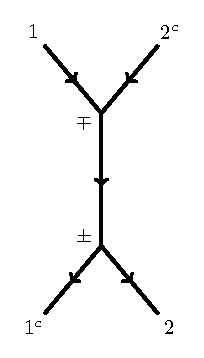
\includegraphics{Figures/Figure_1}
    \caption{ Superdiagrama de menor orden en una colisión spartícula-antispartícula.}
 \label{Figure 1}
 \end{center}
\end{figure}
\begin{IEEEeqnarray}{rl}
            1\rightarrow\pm, \quad 1^{c}\rightarrow\mp,  \quad 2\rightarrow\mp, \quad 2^{c}\rightarrow\pm \ .
    \label{8-01-06}
\end{IEEEeqnarray}
Los signos de arriba(abajo) corresponden a los casos $ g_{-} = 0$($ g_{+} = 0$). La función de onda en el espacio de momentos en el caso del supercampo escalar, es simplemente [ver las Ecs. \eqref{5-3-29} and \eqref{5-3-29}]: 
\begin{IEEEeqnarray}{rl}
            u\left(\mathbf{p} \right)   \, = \,    v\left(\mathbf{p} \right)    \, = \,\frac{1}{\sqrt{2p^{0}}},\quad p^{0} \, = \, \sqrt{\mathbf{p}^{2}  \, + \, m^{2}} \ .
    \label{8-01-07}
\end{IEEEeqnarray}
La contribución de las patas externas al superdiagrama  es 
\begin{IEEEeqnarray}{rl}
     (2\pi)^{-6}\, u(\textbf{p}_{_{2}}) u(\textbf{p}^{c}_{_{1}}) u(\textbf{p}^{c}_{_{2}}) u(\textbf{p}_{_{1}})\,  \times \,       e^{+i x_{_{1}}\cdot\left(  p_{_{1}} -p^{c}_{_{2}}  \right) }   \,   e^{+i x_{_{2}}\cdot \left( p^{c}_{_{1}}  \, - \, p_{_{2}}\right)   }  \nonumber \\
    \times \,\, e^{ 2\left[ {s}_{_{1}}\cdot(+i\slashed{p}_{_{1}})     \, - \, s_{_{2}}^{c}\cdot\, (+i\slashed{p}^{c}_{_{2}})\, \right]{\vartheta}_{_{1}\mp} }\times        e^{  2\left[ {s}_{_{1}} ^{c} \cdot\, (+i\slashed{p}^{c}_{_{1}}) \, - \,{s}_{_{2}} \cdot \, (+i\slashed{p}_{_{2}})\right] \,\vartheta_{_{2}\pm}}\ . \nonumber \\
    \label{8-01-08}
\end{IEEEeqnarray}
Al escribir las exponenciales fermiónicas  hemos usado el hecho de que el  superpotencial $ \mathcal{W}_{\pm} $ esta evaluado en $ (x,\vartheta_{\pm}) $. La contribución de los vértices y la línea interna es
\begin{IEEEeqnarray}{rl}
           \left( 9\times 4\right)  \times \left[ \left( +i\right)^{2} \left( -i\right)^{2}  \left(3! \right)^{-2}  \vert g_{\pm}\vert^{2}\right] \times \left[  \left(-i\right) \left(2\pi \right)^{-4}  \int d^{4}q   \frac{ e^{i\left( x_{_{1}}-x_{_{2}}\right)  \cdot q \, - \, 2\vartheta_{_{1}}^{\intercal}\epsilon\gamma_{5}i\slashed{q}\vartheta_{_{2}\pm}}}{m^{2}+q^{2}-i\varepsilon}\right] \ . \nonumber \\
    \label{8-01-09}
\end{IEEEeqnarray} 
El factor  $ \left( 9\times 4\right)  $,  surge de las posibles combinaciones de formar las lineas internas y externas. Para obtener la superamplitud debemos integrar con 
\begin{IEEEeqnarray}{rl}
            \int d^{4}x_{_{1}}d^{4}x_{_{2}}\,d^{2}\vartheta_{_{1}\mp}\, d^{2}\vartheta_{_{2}\pm} \ .
    \label{8-01-10}
\end{IEEEeqnarray}
Notamos que las integrales de las variables bosónicas nos dan
\begin{IEEEeqnarray}{rl}
              \int d^{4}x_{_{1}} e^{+i x_{_{1}}\cdot\left(  p_{_{1}} -p^{c}_{_{2}}  \, + \, q  \right) }   & \, = \, \left( 2\pi\right)^{4}\delta^{4}\left(  p_{_{1}} -p^{c}_{_{2}}  \, + \, q  \right) \  , \nonumber \\
               \int d^{4}x_{_{2}}   \,   e^{+i x_{_{2}}\cdot \left( p^{c}_{_{1}}  \, - \, p_{_{2}}  \, - \,q\right)   }    &           \, = \, \left( 2\pi\right)^{4}\delta^{4}\left(  p^{c}_{_{1}} -p_{_{2}}  \, - \, q  \right)\ .
    \label{8-01-11}
\end{IEEEeqnarray}
Después de integrar con $ d^{4}q $, obtenemos la expresión siguiente para el superdiagrama \textit{sin} las variables fermiónicas $ \vartheta_{_{1}\mp}$ y  $\vartheta_{_{2}\pm} $ integradas:
\begin{IEEEeqnarray}{rl}
\,\tfrac{1}{4} f_{\text{scalar}} \left( \textbf{p}_{_{1}},\textbf{p}^{c}_{_{1}},\textbf{p}_{_{2}},\textbf{p}^{c}_{_{2}}\right) \, e^{ - 2i {\vartheta}_{{1}\mp}\cdot\left(\slashed{p}_{{1}} {s}_{{1}}   \, - \, \, \slashed{p}^{c}_{2}s_{2}^{c}\, \right)  }      e^{ - 2i\vartheta_{_{2}\pm}\cdot\left(  \, \slashed{p}^{c}_{1}{s}_{1} ^{c}\, - \,  \slashed{p}_{_{2}}{s}_{2}\right) \,}     e^{ \, - \, 2i \vartheta_{_{1}}\cdot \left( \slashed{p}^{c}_{{1}} - \slashed{p}_{{2}}  \right) \vartheta_{_{2}\pm} } \ , \nonumber \\
    \label{8-01-12}
\end{IEEEeqnarray}
con 
\begin{IEEEeqnarray}{rl}
              f_{\text{scalar}} \left( \textbf{p}_{_{1}},\textbf{p}^{c}_{_{1}},\textbf{p}_{_{2}},\textbf{p}^{c}_{_{2}}\right)  &  \, = \,  \left(-4i\right) \vert g_{\pm}\vert^{2}  (2\pi)^{-2}  \,    \delta^{4}\left(  p_{{1}} \, + \,  p^{c}_{{1}} -p^{c}_{{2}}  -p_{{2}}   \right)           \nonumber \\
            & \qquad \times  u(\textbf{p}_{_{2}}) u(\textbf{p}^{c}_{_{1}}) u(\textbf{p}^{c}_{_{2}}) u(\textbf{p}_{_{1}})\,    \times  \left[ {m^{2}+\left( p^{c}_{{1}} -p_{{2}}  \right) ^{2}-i\varepsilon}\right]^{-1}\ .\nonumber \\
    \label{8-01-13}
\end{IEEEeqnarray}
Esta última cantidad, es la expresión para el mismo diagrama pero en el espacio. 
Aislamos la dependencia en la variable $ (\vartheta_{_{1}\mp}) $  e integramos sobre esta variable:
\begin{IEEEeqnarray}{rl}
 \int d^{2}\vartheta_{_{1}\mp}\, e^{ - 2i {\vartheta}_{{1}\mp}\cdot\left[\slashed{p}_{{1}} {s}_{{1}}   \, - \, \, \slashed{p}^{c}_{{2}}s_{{2}}^{c}\, \, + \,  \left( \slashed{p}^{c}_{{1}} - \slashed{p}_{{2}}  \right)\vartheta_{{2}}\right]}    & \, = \, -4\, \delta^{2}\left[\slashed{p}_{{1}} {s}_{{1}}   \, - \, \, \slashed{p}^{c}_{{2}}s_{{2}}^{c}\, \, + \,  \left( \slashed{p}^{c}_{{1}} - \slashed{p}_{{2}}  \right)\vartheta_{{2}}\right]_{\mp}    \nonumber \\
   \, = \,4\left( {p}^{c}_{{1}} - {p}_{{2}}  \right) ^{2} &\delta^{2}\left[ \left( \slashed{p}^{c}_{{1}} - \slashed{p}_{{2}}  \right)^{-1}\left( \slashed{p}_{{1}} {s}_{{1}}   \, - \, \, \slashed{p}^{c}_{{2}}s_{{2}}^{c}\right)\, \, + \,  \vartheta_{{2}}\right]_{\mp}    \ .   \nonumber \\
    \label{8-01-14}
\end{IEEEeqnarray}
Después de integrar con esta función delta  en la variable $ \vartheta_{_{2}\pm}  $, obtenemos la forma final de la superamplitud para la colisión spartícula-antispartícula:
\begin{IEEEeqnarray}{rl}
S^{\mp}\left( \cdots\right)  \, = \, f_{\text{scalar}}\, \times \, \left( {p}^{c}_{{1}} - {p}_{{2}}  \right) ^{2}\times \exp{\left[-2i \, h^{\mp}\left( \cdots\right) \right]} \ ,  \nonumber \\           
    \label{8-01-15}
\end{IEEEeqnarray}
los puntos $ \left( \cdots\right)  $ denotan al superespacio de momentos $  \left(\textbf{p}_{_{1}},s_{_{1}\pm},\textbf{p}^{c}_{_{1}}, s^{c}_{_{1}\mp},\textbf{p}_{_{2}},s_{_{2}\mp},\textbf{p}^{c}_{_{2}}, s^{c}_{_{2}\pm}\right)  $, mientras que la funciones $ h^{\mp} $ vienen dadas por 
\begin{IEEEeqnarray}{rl}
            h^{\mp}\left( \cdots\right)  \, = \, \frac{1}{\left( {p}^{c}_{{1}}  \, - \,{p}_{{2}}  \right)^{2}}\left( \slashed{p}_{{1}} {s}_{{1}}   \, - \, \, \slashed{p}^{c}_{{2}}s_{{2}}^{c}\right) \cdot \left( \slashed{p}^{c}_{{1}} - \slashed{p}_{{2}}  \right)\left(  \, \slashed{p}^{c}_{1}{s}_{1} ^{c}\, - \,  \slashed{p}_{_{2}}{s}_{2}\right)_{\pm}\ .\nonumber \\
    \label{8-01-16}
\end{IEEEeqnarray} 

 La posibilidad de escoger  tres partículas  y tres antipartículas  para la dispersión partícula-antipartícula  nos da un total de $ 3^{4} $ combinaciones de estados iniciales y finales. Desde luego que muchos  de estos procesos son cero, por ejemplo, todos los procesos que provienen de la expansión impar en las variables fermiónicas en la Ec. \eqref{8-01-16} (esto no es otra cosa que una consecuencia que la conservación de momento angular). Vemos de manera explícita la conveniencia de trabajar en una formulación completamente en el superespacio; la  ecuación \eqref{8-01-16} representa una expresión económica para el conjunto de todos los procesos de estas partículas a segundo orden  en la constante de acoplamiento $ \vert  g_{\pm}\vert $.\\

\section{Equivalencia con el Modelo de Wess-Zumino}\label{Sec_TimeOrderedSuperpropagators}
\label{sec:08-02}
Para establecer una equivalencia entre la formulación nocanónica (aquí desarrollada) y la formulación canónica, escribimos el superpropagador no corregido para el supercampo escalar, como aparece en los superpotenciales quirales  (por ahora, hemos omitido un factor de $ -i $):
\begin{IEEEeqnarray}{rl}
  \delta^{2}(\vartheta_{_{1}\mp})\delta^{2}  (\vartheta_{_{2}\pm}) &\tilde{\Delta}^{\pm \mp}\left( x_{_{1}},\vartheta_{_{1}},x_{_{2}},\vartheta_{_{2}}\right)  \nonumber\\
       \, = \,  \delta^{2} & (\vartheta_{_{1}\mp})\delta^{2}  (\vartheta_{_{2}\pm}) \left[1  \, +\, 2 \vartheta_{_{1}}\cdot(-\slashed{\partial}_{_{1}})\vartheta_{_{2}\mp}  \, - \,4 m^{2}\,\delta^{2}(\vartheta_{_{1}\pm})\delta^{2}  (\vartheta_{_{2}\mp})  \right] \Delta_{F}(x_{_{1}}-x_{_{2}}) \ .\nonumber \\  
    \label{08-02-01}
\end{IEEEeqnarray}
Haciendo uso de $ \left( \square - m^{2}\right)\Delta_{F}(x)  \, = \, -\delta^{4}(x) $, escribimos
\begin{IEEEeqnarray}{ll}
  \delta^{2}(\vartheta_{_{1}\mp})\delta^{2}  (\vartheta_{_{2}\pm}) &\tilde{\Delta}^{\pm \mp}\left( x_{_{1}},\vartheta_{_{1}},x_{_{2}},\vartheta_{_{2}}\right)   \nonumber\\
  &  \, = \,\delta^{2}(\vartheta_{_{1}\mp})\delta^{2}  (\vartheta_{_{2}\pm}) \,  \Delta_{F}\left( x^{\pm}_{_{12}}\right)  \, - \, 4  \,\delta^{4}(\vartheta_{_{1}})\,\delta^{4}  (\vartheta_{_{2}})\delta^{4}(x_{_{1}}-x_{_{2}}) \ .  \nonumber \\
    \label{08-02-02}
\end{IEEEeqnarray}
El término $ \, +\, 4 i\,\delta^{4}(\vartheta_{_{1}})\delta^{4}  (\vartheta_{_{2}})\delta^{4}(x_{_{1}}-x_{_{2}}) $ es invariante de Lorentz pero no invariante supersimétrico. Puesto que esta expresión es local en el superespacio, la parte no-covariante del superpropagador  induce términos no covariantes en las interacciones. En el caso de superpotenciales de supercampos arbitrarios, para darnos una idea de su forma, recordamos que aunque la función paso es invariante de Lorentz (excepto en separaciónes del tipo-espacial, donde para lograr la invariancia de Lorentz los conmutadores deben de hacerse cero) no es invariante supersimétrica.  La función paso $ \omega $ seria invariante supersimétrica, si estuviese evaluada en  $   x^{\pm\,0}_{_{12}} $ o incluso en  $  x^{0}_{_{12}}-\vartheta_{_{1}}\cdot\gamma^{0}\vartheta_{_{2}} $. Tomando en cuenta que las funciones  $ \Delta_{+} $ que aparecen en la Ec. \eqref{08-02-02} están evaluadas en  $   x^{\pm\,0}_{_{12}} $, escribimos 
\begin{IEEEeqnarray}{rl}
              \omega\left( x^{0}_{_{12}}\right) \, = \,  \omega\left(  x^{\pm\,0}_{_{12}} \right) \, + \, \varsigma_{\pm} \left( z_{_{1}},z_{_{2}}\right) , \quad z=(x,\vartheta) \ .
      \label{08-02-03}
  \end{IEEEeqnarray}
Aquí,    $ \varsigma_{\pm }  \left( z_{_{1}},z_{_{2}}\right) $  es el negativo de los coeficientes   de orden mayor que cero  en la expansión en serie de Taylor de las variables fermiónicas  en  $ \omega\left(  x^{\pm\,0}_{_{12}} \right)$. El operador unitario a segundo orden en la serie de Dyson está dado por 
  \begin{IEEEeqnarray}{rl}
                U^{(2)}  & \, = \,{{(-i)^{2}}}\int d^{8}z_{_{1}}d^{8}z_{_{2}}\, \omega\left( x^{0}_{_{12}}\right) \mathcal{H}(z_{_{1}}) \mathcal{H}(z_{_{2}})   \ .
    \label{08-02-04}
\end{IEEEeqnarray} 
Para el caso de los superpotenciales, esta última expresión queda como 
\begin{IEEEeqnarray}{rl}
                U^{(2)}                 
                   & \, = \,{{(-i)^{2}}}\int d^{8}z_{_{1}}d^{8}z_{_{2}}\,       \left[ \omega\left( x^{0}_{_{12}}\right) \mathcal{H}_{\pm}(z_{_{1}})\mathcal{H}^{*}_{\mp }(z_{_{2}})   \, + \,           \omega\left( x^{0}_{_{12}}\right)\mathcal{H}^{*}_{\mp }(z_{_{1}})\mathcal{H}_{\pm}(z_{_{1}})   \, + \, \dots\right]    \nonumber \\   
              & \, = \,    U_{\text{i}}^{(2)}   \, + \, U_{\text{n.i}}^{(2)}   \, + \, \dots \ ,
    \label{08-02-05}
\end{IEEEeqnarray} 
con el término covariante de super Poincar\'e 
\begin{IEEEeqnarray}{rl}
               U_{\text{i}}^{(2)}    & \, = \,  {{(-i)^{2}}}\int d^{8}z_{_{1}}d^{8}z_{_{2}}\,\left(   \omega\left(  x^{\pm\,0}_{_{12}} \right)   \mathcal{H}_{\pm}(z_{_{1}}) \mathcal{H}^{*}_{\mp}(z_{_{2}})   \, + \,   \omega\left( x^{\mp\,0}_{_{21}} \right) \mathcal{H}^{*}_{\mp}(z_{_{2}}) \mathcal{H}_{\pm}(z_{_{1}})  \right)  \nonumber 
               \\ 
       \label{08-02-06}
   \end{IEEEeqnarray} 
y el término no covariante
   \begin{IEEEeqnarray}{rl}
               U_{\text{n.i}}^{(2)}    & \, = \,  {{(-i)^{2}}}\int d^{8}z_{_{1}}d^{8}z_{_{2}}\left( \,\varsigma_{\pm} \left( z_{_{1}},z_{_{2}}\right)   \mathcal{H}_{\pm}(z_{_{1}}) \mathcal{H}^{*}_{\mp}(z_{_{2}})   \, + \,  \varsigma_{\mp} \left( z_{_{2}},z_{_{1}}\right) \mathcal{H}^{*}_{\mp}(z_{_{2}}) \mathcal{H}_{\pm}(z_{_{1}})  \right)    \ .  \nonumber \\
       \label{08-02-07}
   \end{IEEEeqnarray}    
   Debido a las funciones delta fermiónicas en los superpotenciales, podemos evaluar las funciones paso en   $ \left( x^{0}_{_{12}} \, - \, 2 \vartheta_{_{1}\pm}\cdot\gamma^{0}\vartheta_{_{2}\mp}\right)  $, permitiendonos escribir la parte no covariante de las funciones paso como 
\begin{IEEEeqnarray}{rl}
                           \varsigma_{\pm}\left(z_{_{1}},z_{_{2}}  \right)            &  \,=\, 2  \vartheta_{_{1}\pm }\cdot\gamma^{0}\vartheta_{_{2}\mp }\,\delta\left( x^{0}_{_{12}}    \right) \, - \, 4\,\delta^{2}(\vartheta_{_{1}\pm }) \,\delta^{2}(\vartheta_{_{2}\mp }) \, \frac{\partial}{\partial x_{_{1}}^{0}}\,\delta\left( x_{_{12}}^{0}  \right)     \ .    \nonumber \\
                 \label{08-02-08}
             \end{IEEEeqnarray}   
             Podemos ver de esta expresión, que los otros términos [expresados como $ \dots$ en \eqref{08-02-05}] no necesitan ser corregidos. Notando  que  $    \varsigma_{-}\left(z_{_{1}},z_{_{2}}  \right)  \, = \,    -\varsigma_{+}\left(z_{_{2}},z_{_{1}}  \right)     $, escribimos
\begin{IEEEeqnarray}{rl}
       U_{\text{n.i}}^{(2)} & \, = \,      {{(-i)^{2}}}\int d^{8}z_{_{1}}d^{8}z_{_{2}}\,  \varsigma_{\pm}\left( z_{_{1}},z_{_{2}}\right)    \left[  \mathcal{V}_{\pm}(z_{_{1}}),  \mathcal{V}^{*}_{\mp}(z_{_{2}})   \right] \ .
    \label{08-02-09}
\end{IEEEeqnarray}  
Escribimos el superpotencial general  en componentes:
\begin{IEEEeqnarray}{l}
            \mathcal{W}_{\pm}(x,\vartheta)   \, = \, \mathcal{C}\left(x_{\pm} \right)   \, + \, \sqrt{2}\,\vartheta_{\pm}\cdot\gamma_{5} \,\Omega\left(x_{\pm} \right)   \, +  \, \delta^{2}(\vartheta_{\pm}){\vartheta\cdot \vartheta_{\pm}}\,\mathcal{F}\left(x_{\pm} \right)  \ . \nonumber \\
    \label{08-02-10}
\end{IEEEeqnarray} 
Integramos sobre las variables fermiónicas en  \eqref{08-02-09}, para obtener
\begin{IEEEeqnarray}{rl}
       U_{\text{n.i}}^{(2)} & \, = \,     +4\int d^{4}x_{_{1}}d^{4}x_{_{2}}\, \left(  i \delta\left( x^{0}_{_{12}} \right) \sum_{\alpha}\left\lbrace \left[ \Omega\left(x_{{_{1}}} \right)\right] _{\pm\alpha} ,    \left[\Omega^{*}\left(x_{{_{2}}} \right)\right]_{\pm\alpha}\right\rbrace \right.  \nonumber \\
      &\qquad  \qquad    \qquad \qquad\qquad \left.  \, + \,  \, \delta\left( x_{_{12}}^{0}  \right) \frac{\partial}{\partial x_{_{1}}^{0}}\, \left[  \mathcal{C}\left(x_{_{1}} \right)  ,   \mathcal{C}^{*}\left(x_{_{2}}\right) \right] \right)  \ .
    \label{08-02-11}
\end{IEEEeqnarray} 
Cualquier (anti)conmutador generará productos de campos multiplicados por las funciones  $ \Delta(x) = \Delta_{+}(x) \, - \, \Delta_{+}(-x) $ y sus derivadas.  Debido a  las funciones delta en el tiempo y a  $ \left( \square\Delta(x)= m^{2}\Delta(x) \right) $, los únicos términos que sobreviven en el anticonmutador(conmutador) de la Ec.  \eqref{08-02-11}, son aquellos  en los que un número (impar)par de derivadas temporales actúan sobre  $  \Delta(x) $, generando funciones delta $\delta(x^{0}_{_{12}})\frac{\partial}{\partial x_{_{1}}^{0}}\Delta\left(x_{_{1}}- x_{_{2}}\right) = -i\delta^{4}(x_{_{1}}-x_{_{2}})  $. Esto nos permite escribir 
\begin{IEEEeqnarray}{rl}
       U_{\text{n.i}}^{(2)} %& \, = \,   -i   
        & \, = \,  i  \int d^{4}x_{_{1}}d^{4}x_{_{2}}  \,\delta^{4}(x_{_{1}}-x_{_{2}}) F\left(x_{_{1}}\right)  \ ,
    \label{08-02-12}
\end{IEEEeqnarray} 
con $  F\left(x_{_{1}}\right)    $ dada explicitamente por el término del factor integral de  $ d ^{4}x_{_{1}} $ en \eqref{08-02-11}.  Entonces, debemos reemplazar
\begin{IEEEeqnarray}{rl}
               \mathcal{V}\left( x,\vartheta\right) \, \rightarrow  \,  \mathcal{V}\left( x,\vartheta\right)  \, + \, \delta^{4}\left(\vartheta \right) F\left( x\right) \ ,
    \label{08-02-13}
\end{IEEEeqnarray}
de manera que cancelemos el término no covariante a menor orden \eqref{08-02-11}. Es evidente que este resultado se extiende para el caso de potenciales generales, puesto que el efecto de considerar la expansión completa en las variables fermiónicas, es generar derivadas de mayor orden en el tiempo. Como hemos argumentado en la sección \ref{chap:6-4}, el punto importante es que siempre tenemos una función delta $\delta(x_{_{1}}^{0}-x_{_{2}}^{0})$, asegurándonos contratérminos locales en el tiempo, nuestra suposición principal. La  función $   F\left(x_{_{1}}\right)     $  es en general, no solo supersimetricamente no covariante sino también Lorentz no covariante. Para el caso del supercampo escalar, todos los contratérminos son covariantes de Lorentz. De las Ecs. \eqref{8-01-05} y \eqref{08-02-10}, podemos ver que 
 \begin{IEEEeqnarray}{rl}
             \mathcal{C}\left(x \right)  &\, = \, \frac{g_{+}}{3!}  \left( \phi_{+}\right)^{3}  \, + \, \frac{g_{-}}{3!}\left( \phi^{*}_{-}\right)^{3}\ , \nonumber \\
 \Omega\left(x\right)   &\, = \ -\frac{g_{+}}{2}  \left(  \phi_{+} \right) ^{2}\psi  \, + \, \frac{g_{-}}{2} \left(  \phi^{*}_{-} \right) ^{2}\left[ \epsilon\gamma_{5}\beta  \psi^{*}\right]  \ , \nonumber \\
 \mathcal{F}\left(x \right)    &\, = \,{g_{+}} \left( -  \phi_{+} \psi ^{\intercal}    \epsilon\psi_{+}    \, + \,   m\left( \phi_{+}\right)^{2} \phi_{-}\right)\nonumber \\
 &\qquad    \, + \, {g_{-}}\left(-  \phi^{*}_{-} \psi ^{\dagger}    \epsilon\psi^{*}_{-}    \, + \,  m \left( \phi^{*}_{-}\right)^{2} \phi^{*}_{+} \right)  \ .  
    \label{08-02-15}
\end{IEEEeqnarray}
Para este superpotencial, las correcciones a orden menor [ver Ec. \eqref{08-02-11}] son~\footnote{Para prepararnos  para la teoría del campo, hemos ignorado los términos bilineales  cuando trajimos el término $   \left[  \mathcal{C}\left(x_{_{1}}\right) , \mathcal{C}^{*}\left(x_{_{2}}\right)\right]   $, a la forma  \eqref{08-02-15}.}
\begin{IEEEeqnarray}{rl}
    i\delta\left(x^{0}_{_{12}} \right)  \sum_{\alpha}\left\lbrace \left[ \Omega\left(x_{{_{1}}} \right)\right] _{\pm\alpha} ,    \left[\Omega^{*}\left(x_{{_{2}}} \right)\right]_{\pm\alpha}\right\rbrace  & \, = \,      -2 \delta\left( {x_{_{12}}^{0}} \right) \tfrac{\partial}{\partial x^{0}_{_{1}}}    \left[  \mathcal{C}\left(x_{_{1}}\right) , \mathcal{C}^{*}\left(x_{_{2}}\right)\right]    \nonumber \\    
           &   \, = \,     
              \tfrac{1}{2} \left[ i\delta^{4}\left(x_{_{1}}-x_{_{2}}\right)  \right] \, F\left( x_{_{2}}\right)  \  , \label{CommutatorCorrections}
\end{IEEEeqnarray}
donde $  F\left( x_{_{2}}\right) $  es la función que aparece en  \eqref{08-02-12} y esta dada por 
\begin{IEEEeqnarray}{rl}
             F\left(  x_{_{2}}\right)  \, = \,  \vert g_{+} \vert^{2}\left( \phi_{+}\left(x_{_{2}}\right) \right)^{2} \left( \phi^{*}_{+}\left(x_{_{2}}\right) \right)^{2}   \, + \,  \vert g_{-} \vert^{2}\left( \phi_{-}\left(x_{_{2}}\right) \right)^{2} \left( \phi^{*}_{-}\left(x_{_{2}}\right) \right)^{2}  \ .
     \label{FirstCorrectionToThePotentials}
 \end{IEEEeqnarray}
El potencial covariante en el espacio, 
\begin{IEEEeqnarray}{rl}
           -i V\left(x\right)    &  \, = \,   \mathcal{F}\left(x \right)  \, - \, \, \mathcal{F}\left(x \right) ^{*} \ ,
    \label{08-02-16}
\end{IEEEeqnarray}
adquiere la forma 
\begin{IEEEeqnarray}{rl}
           -i V\left(x\right)    
             & \, = \,  {g_{+}} \left( -  \phi_{+}\psi ^{\intercal}    \epsilon\psi_{+}   + \, m \ \left( \phi_{+}\right)^{2} \phi_{-}\right)  \, + \, 
  {g_{-}}\left( - \phi_{-} \psi ^{\intercal}    \epsilon\psi_{-}    \, - \,   m\left( \phi_{-}\right)^{2} \phi_{+}\right) \nonumber \\
 & \qquad  \, + \, {g^{*}_{-}}\left(- \phi^{*}_{-} \psi ^{\dagger}    \epsilon\psi^{*}_{-}    \, + \, m  \left( \phi^{*}_{-}\right)^{2} \phi^{*}_{+} \right)  \, + \, {g^{*}_{+}}\left(-\phi^{*}_{+} \psi ^{\dagger}    \epsilon\psi^{*}_{+}    \, -\, m \left( \phi^{*}_{+}\right)^{2} \phi^{*}_{-} \right) \ .\nonumber \\
    \label{08-02-17}
\end{IEEEeqnarray}
 Finalmente, después de integrar las variables fermiónicas  en la Ec.  \eqref{08-02-13}, el potencial  resultante  (corregido) en el espaciotiempo es:
\begin{IEEEeqnarray}{rl}
             -\mathcal{H}_{\text{int}} \left(x\right)  & \, = \,  - F\left( x\right)   \, - \,V\left(x\right)    \nonumber \\ 
   &\, = \,    -i{g_{+}} \left( -  \phi_{+}\psi ^{\intercal}    \epsilon\psi_{+}   + \, m \ \left( \phi_{+}\right)^{2} \phi_{-}\right)  \, - \, i{g_{-}}\left( - \phi_{-} \psi ^{\intercal}    \epsilon\psi_{-}    \, - \,   m\left( \phi_{-}\right)^{2} \phi_{+}\right) \nonumber \\
 & \qquad  \, - \, i{g^{*}_{-}}\left(- \phi^{*}_{-}  \psi  ^{\dagger}    \epsilon\psi^{*} _{-}    \, + \, m  \left( \phi^{*}_{-} \right)^{2} \phi ^{*}_{+} \right)   \, - \, i{g^{*}_{+}}\left(-\phi^{*}_{+}  \psi  ^{\dagger}    \epsilon\psi^{*}  _{+}    \, -\, m \left( \phi^{*}_{+}\right)^{2} \phi^{*}_{-}   \right)  \nonumber \\
   &\qquad -\left( \vert g_{+} \vert^{2}\left( \phi_{+}\right) ^{2}\left( \phi^{*}_{+}  \right) ^{2}  \, + \, \vert g_{-}  \vert^{2}\left( \phi_{-}\right) ^{2}\left( \phi^{*}_{-}  \right) ^{2}\right) \ .
    \label{08-02-18}
\end{IEEEeqnarray}

\begin{center}
\textit{\textbf{El formalismo canónico}} 
\end{center}


 Antes de hacer el comparativo explícito del potencial obtenido [Ec. \eqref{08-02-18}] con el  modelo de Wess-Zumino,  es necesario primero  exponer los rudimentos del formalismo canónico. Comenzamos escribiendo la acción en términos de su Lagrangiana, esta a su vez es escrita en términos de la densidad Lagrangiana en el superespacio:
\begin{IEEEeqnarray}{rl}
            \mathcal{A}  & \, = \, \int dt L\ , \nonumber \\
          L  & \, = \,    \int d^{3}x d^{4}\vartheta \, \mathcal{L} \left(\Phi, \partial_{\mu}\Phi \right) \ .
    \label{08-02-a01}
\end{IEEEeqnarray}
Debido a la condición de quiralidad de los supercampos, hacemos
\begin{IEEEeqnarray}{rl}
            \Phi_{\pm \ell}  \, = \, \mathcal{D}^{2}_{\mp} S_{\pm \ell}, \quad  \Phi^{\dagger}_{\pm}  \, = \,- \mathcal{D}^{2}_{\mp} S^{\dagger}_{\pm \ell}\ , 
    \label{08-02-a02}
\end{IEEEeqnarray}
con $  \mathcal{D}^{2}_{\pm}   \, = \, \frac{1}{2}\mathcal{D}^{\intercal}\epsilon \mathcal{D}_{\pm} $ y 
donde  $ S_{\pm \ell} $ son campos generales sin restricciones (los cuales podemos variar arbitrariamente), el índice  $ \ell $ representa el tipo de supercampo (escalar, espinorial,  vectorial, etc.). Variamos la acción con respecto a estos supercampos:
\begin{IEEEeqnarray}{rl}
          \delta  \mathcal{A}  \, = \, \sum_{\varepsilon,\ell}\int d^{4}x d^{4}\vartheta  \, \left\lbrace \mathcal{D}^{2}_{-\varepsilon}\left[ \frac{\delta {L} }{\delta \Phi_{\varepsilon \ell}}  \, - \,\frac{d}{dt}  \frac{\delta {L} }{\delta \dot{\Phi}_{\varepsilon \ell}} \right]\right\rbrace \,\delta S_{\varepsilon \ell} \ .
    \label{08-02-a03}
\end{IEEEeqnarray}
No hemos realizado las variaciones con respecto a los supercampos  conjugados  $ S^{\dagger}_{\pm \ell} $, porque estamos suponiendo que la Lagrangiana es real; las ecuaciones del movimiento que surgen de las variaciones de los supercampos adjuntos serán simplemente el adjunto de las ecuaciones del  movimiento de los supercampos (sin conjugar). Puesto que 
\begin{IEEEeqnarray}{rl}
             \frac{\delta  \mathcal{L} }{\delta \Phi_{\varepsilon \ell}} &\, = \,  \frac{\partial \mathcal{L} }{\partial  \Phi_{\varepsilon \ell}}  \, - \, \nabla \cdot \frac{\partial \mathcal{L} }{\partial \nabla  \Phi_{\varepsilon \ell}}\ , \nonumber   \\
             \frac{\delta  \mathcal{L} }{\delta \dot{\Phi}_{\varepsilon \ell}} &\, = \,  \frac{\partial \mathcal{L} }{\partial  \dot{\Phi}_{\varepsilon \ell}}  \ ,
    \label{08-02-a04}
\end{IEEEeqnarray}
tenemos que 
\begin{IEEEeqnarray}{rl}
          \delta  \mathcal{A}  \, = \, \sum_{\varepsilon,\ell}\int d^{4}x d^{4}\vartheta  \, \left\lbrace \mathcal{D}^{2}_{-\varepsilon}\left[ \frac{\partial}{\partial x^{\mu}}\frac{\partial \mathcal{L}}{\partial \left(\partial \Phi_{\varepsilon \ell}/\partial x^{\mu} \right) }   \, - \,\frac{\partial\mathcal{L}}{\partial \Phi_{\varepsilon \ell} }\right]\right\rbrace \,\delta S_{\varepsilon \ell}   \ .\nonumber \\
    \label{08-02-a05}
\end{IEEEeqnarray}
Hacemos la partición de la densidad Lagrangiana en  términos del potencial de K\"{a}hler y el superpotencial $ \mathcal{W}_{\pm} $,
\begin{IEEEeqnarray}{rl}
            \mathcal{L} \left(\Phi, \partial_{\mu}\Phi \right)    \, = \, -\tfrac{1}{4}\mathcal{K} \, + \, \sum_{\varepsilon}^{+,-}\delta^{2}\left(\vartheta_{-\varepsilon} \right) \mathcal{W}_{\varepsilon}\ ,
    \label{08-02-a06}
\end{IEEEeqnarray}
donde 
\begin{IEEEeqnarray}{rl}
            \mathcal{D}_{-\varepsilon}\mathcal{W}_{\varepsilon}  \, = \,  0, \quad  \mathcal{W}^{*}_{-\varepsilon}    \, = \,  -\mathcal{W}_{\varepsilon} \, \quad \mathcal{K}   \, = \,  \mathcal{K}^{*} \ .
    \label{08-02-a07}
\end{IEEEeqnarray}
Podemos ver que:
\begin{IEEEeqnarray}{rl}
             \sum_{\varepsilon',\varepsilon}^{+,-}    \mathcal{D}^{2}_{-\varepsilon} \left\lbrace \,\delta^{2}\left(\vartheta_{-\varepsilon'} \right) \left[ \frac{\partial}{\partial x^{\mu}}\frac{\partial }{\partial \left(\partial \Phi_{\varepsilon \ell}/\partial x^{\mu} \right) }   \, - \,\frac{\partial}{\partial \Phi_{\varepsilon \ell} }\right]  \mathcal{W}_{\varepsilon'}   \right\rbrace  \nonumber \\ 
        \, = \,    - \sum_{\varepsilon}^{+,-}   \left[ \frac{\partial}{\partial x^{\mu}}\frac{\partial }{\partial \left(\partial \Phi_{\varepsilon \ell}/\partial x^{\mu} \right) }   \, - \,\frac{\partial}{\partial \Phi_{\varepsilon \ell} }\right]   \mathcal{W}_{\varepsilon}  \ ,
    \label{08-02-a08}
\end{IEEEeqnarray}
para reescribir  la Ec. \eqref{08-02-a05}  como 
\begin{IEEEeqnarray}{rl}
          \delta  \mathcal{A}  \, = \, \sum_{\varepsilon}\int d^{4}x d^{4}\vartheta  \, \left\lbrace  \left[ \frac{\partial}{\partial x^{\mu}}\frac{\partial }{\partial \left(\partial \Phi_{\varepsilon\ell}/\partial x^{\mu} \right) }   \, - \,\frac{\partial}{\partial \Phi_{\varepsilon\ell} }\right] \left( -\frac{1}{4}\mathcal{D}^{2}_{-\varepsilon}\mathcal{K} \, - \, \mathcal{W}_{\varepsilon}\right) \right\rbrace \,\delta S_{\varepsilon \ell}    \ . \nonumber \\
    \label{08-02-a09}
\end{IEEEeqnarray}
Cuando se cumple que  $ \delta  \mathcal{A}  \, = \,0 $, para  variaciones arbitrarias  $ \delta S_{\varepsilon \ell}   $, tenemos que el término entre llaves en la Ec. \eqref{08-02-a09} tiene que ser cero, esto es, 
\begin{IEEEeqnarray}{rl}
            \left[ \frac{\partial}{\partial x^{\mu}}\frac{\partial }{\partial \left(\partial \Phi_{\varepsilon\ell}/\partial x^{\mu} \right) }   \, - \,\frac{\partial}{\partial \Phi_{\varepsilon\ell} }\right] \left(\tfrac{1}{4} \mathcal{D}^{2}_{-\varepsilon}\mathcal{K} \, +\, \mathcal{W}_{\varepsilon}\right)   \, = \,  0\ ,\quad 
    \label{08-02-a10}
\end{IEEEeqnarray}
Nos restringimos a potenciales de K\"ahler renormalizables y superpotenciales que no dependen de las derivadas ordinarias (covariantes), esto es, 
\begin{IEEEeqnarray}{rl}
            \mathcal{K}  &\, = \,  \Phi^{\dagger}_{-}\Phi_{+}  \, + \, \Phi^{\dagger}_{+}\Phi_{-}, \nonumber \\
    \label{08-02-a11}
\end{IEEEeqnarray}
y
\begin{IEEEeqnarray}{rl}
            \frac{\partial\, \mathcal{W}_{\pm}}{\partial  \left(\partial \Phi_{\pm \ell}/\partial x^{\mu} \right) }    \, = \, 0\ .
    \label{08-02-a12}
\end{IEEEeqnarray}
En este caso, las ecuaciones del movimiento se ven como 
\begin{IEEEeqnarray}{rl}
            \tfrac{1}{4} \mathcal{D}^{2}_{\mp}\Phi^{*}_{\mp \ell} \, = \,   - \frac{\partial \mathcal{W}_{\pm}}{\partial  \Phi_{\pm \ell} },\quad  \tfrac{1}{4} \mathcal{D}^{2}_{\mp}\Phi_{\mp \ell} \, = \,   - \frac{\partial \mathcal{W}_{\pm}}{\partial  \Phi^{\dagger}_{\pm \ell} } \ .
    \label{08-02-a13}
\end{IEEEeqnarray}
Expandiendo los supercampos $ {\Phi}_{\pm \ell} $ de la siguiente manera:
\begin{IEEEeqnarray}{rl}
             {\Phi}_{\pm \ell} & \, = \, \phi_{\pm \ell}   \, - \,  \sqrt{2}\vartheta_{\pm}^{\intercal}\epsilon\, \psi_{\pm \ell}\, \pm \, \vartheta^{\intercal}_{\pm}\epsilon \vartheta_{\pm}\, \mathcal{F}_{\pm \ell}\ , \nonumber \\
               {\Phi}^{*}_{\pm \ell}      & \, =\, \phi^{*}_{\mp \ell}   \, - \,  \sqrt{2} \vartheta_{\pm}^{\intercal} \epsilon\left[(-)^{\Phi+1} \epsilon\gamma_{5}\beta\psi^{*}_{\mp \ell}\right] \, \pm \, \vartheta^{\intercal}_{\pm}\epsilon \vartheta_{\pm}\, \mathcal{F}^{*}_{\mp \ell} \ ,\nonumber \\
     \label{08-02-a14}
 \end{IEEEeqnarray}
tenemos que
\begin{IEEEeqnarray}{rl}
             \mathcal{D}^{2}_{\mp}        {\Phi}_{\mp \ell}\left(x,\vartheta \right)   &  \, = \, \pm 2  \left\lbrace \mathcal{F}_{\mp \ell}\left(x_{\pm} \right)  \, - \,  \sqrt{2}\vartheta_{\pm}^{\intercal}\epsilon \left[ -\slashed{\partial}\psi_{\ell} \left(x_{\pm} \right) \right] \, \pm \, \,  \vartheta^{\intercal}\epsilon\vartheta_{\mp}  \,\square\phi_{\mp \ell}\left(x_{\pm}\right) \right\rbrace \ ,\nonumber \\
              \mathcal{D}^{2}_{\mp}        {\Phi}^{\dagger}_{\mp \ell}\left(x,\vartheta \right)   &  \, = \, \pm 2  \left\lbrace \mathcal{F}^{*}_{\pm \ell}\left(x_{\pm} \right)  \, - \,  \sqrt{2}\vartheta_{\pm}^{\intercal}\epsilon \left[ -\slashed{\partial}(-)^{\Phi_{\ell}+1} \epsilon\gamma_{5}\beta\psi^{*}_{\ell}\left(x_{\pm} \right) \right] \, \pm \, \,  \vartheta^{\intercal}\epsilon\vartheta_{\mp}  \,\square\phi^{*}_{\pm \ell}\left(x_{\pm}\right) \right\rbrace \ .\nonumber \\
    \label{08-02-a15}
\end{IEEEeqnarray} 

El término de orden cero de cualquier función $ F(\Phi_{\pm},\Phi^{\dagger}_{\pm}) $ es simplemente  $ F(\phi_{\pm},\phi^{*}_{\pm}) $, entonces, las ecuaciones del movimiento para las supercampos  auxiliares son 
\begin{IEEEeqnarray}{rl}
            \pm \frac{1}{2}\mathcal{F}^{*}_{\pm \ell}  \, = \,   -\frac{\partial \mathcal{W}_{\pm}(\phi_{\pm},\phi^{*}_{\mp})  }{\partial \phi_{\pm \ell}}, \quad \pm \frac{1}{2}\mathcal{F}_{\mp \ell}  \, = \,   -\frac{\partial \mathcal{W}_{\mp}(\phi_{\mp},\phi^{*}_{\pm})  }{\partial \phi^{* }_{\mp \ell}}\ .
    \label{08-02-a16}
\end{IEEEeqnarray}
O bien, haciendo 
\begin{IEEEeqnarray}{rl}
            \mathcal{W}_{\pm}   \, = \, \pm\frac{1}{2} f\left( \Phi_{\pm},\Phi^{\dagger}_{\pm}\right) \ ,  
    \label{08-02-a17}
\end{IEEEeqnarray}
podemos escribir equivalentemente:
\begin{IEEEeqnarray}{rl}
             \mathcal{F}_{\pm \ell}  \, = \,   -\left( \frac{\partial f(\phi_{\pm},\phi^{*}_{\mp})  }{\partial \phi_{\pm \ell}}\right)^{*} ,  \qquad            \mathcal{F}^{*}_{\mp \ell}  \, = \,   - \left( \frac{\partial f(\phi_{\pm},\phi^{*}_{\mp})  }{\partial \phi^{* }_{\mp \ell}}\right)^{*} \ .
    \label{08-02-a18}
\end{IEEEeqnarray}
En las convenciones que estamos usando, los términos $ D $ y $ \mathcal{F}_{\pm} $ del potencial de K\"ahler y del superpotencial vienen dados  por
\begin{IEEEeqnarray}{rl}
                \int d^{4}x[\cdots]_{D}  &\, = \, -\frac{1}{2}\int d^{4}x d^{4}\vartheta [\cdots] \ , \\
                 \int d^{4}x[\cdots]_{\mathcal{F}_{\pm}}    &\, = \,  \pm \frac{1}{2}\int d^{4}x d^{4}\vartheta \delta(\vartheta_{\mp})[\cdots ] \ , 
     \label{08-02-a20}
 \end{IEEEeqnarray}
 respectivamente. Al integrar en las variables fermiónicas obtenemos la acción en el espacio
\begin{IEEEeqnarray}{rl}
   \mathcal{A}^{\text{espacio}}  \, = \,       \int d^{4}\vartheta \left[  -\tfrac{1}{4}\mathcal{K} \, + \, \delta^{2}\left(\vartheta_{-} \right) \mathcal{W}_{+} \, + \,  \delta^{2}\left(\vartheta_{+} \right) \mathcal{W}_{-}\right]     \nonumber \\
         \, = \,        \frac{1}{2} \int d^{4}x   \left[  \sum_{\ell}\left( \Phi^{*}_{- N}\Phi_{+ \ell}  \, + \, \Phi^{*}_{+ \ell}\Phi_{- \ell}\right) \right]_{\mathcal{D}}   \, + \, \int d^{4}x \left(  \left[  f_{+} \right]_{\mathcal{F}_{+}}  \, + \,    \left[  f_{-} \right]_{\mathcal{F}_{-}}   \right)\ , \nonumber\\
    \label{08-02-a21}
\end{IEEEeqnarray}
Entonces, la Lagrangiana en el espacio viene dada por 
\begin{IEEEeqnarray}{rl}
            \mathcal{L}^{\text{espacio}}  & \, = \,  -\frac{1}{2}\left[  \sum_{\ell}\left( \Phi^{*}_{- \ell}\Phi_{+ \ell}  \, + \, \Phi^{*}_{+ \ell}\Phi_{- \ell}\right) \right]_{\mathcal{D}}    \, + \,  \left[  f_{+} \right]_{\mathcal{F}_{+}}  \, + \,    \left[  f_{-} \right]_{\mathcal{F}_{-}}  \ . \nonumber \\           
    \label{08-02-a22}
\end{IEEEeqnarray}
 Al evaluar los campos auxiliares \eqref{08-02-a18} para obtener la Lagrangiana exclusivamente como función de los campos que se propagan, tenemos
\begin{IEEEeqnarray}{rl}
            \mathcal{L}^{\text{espacio}}         & \, = \, \mathcal{L}^{\text{libre}}  \, + \, \mathcal{L}^{\text{int.}}\ , \nonumber \\
    \label{08-02-a23}
\end{IEEEeqnarray}
 donde 
\begin{IEEEeqnarray}{rl}
            \mathcal{L}^{\text{libre}}  &  \, = \,  -\sum_{\ell}\left(\partial_{\mu}\phi^{\dagger}_{+ \ell} \partial^{\mu}\phi_{+ \ell}   \, + \, \partial_{\mu}\phi^{\dagger}_{- \ell} \partial^{\mu}\phi_{- \ell}   \, + \,\bar{\psi}_{\ell}\slashed{\partial} \psi_{\ell}\right)  \nonumber \\
%     \mathcal{L}^{\text{int.}}       & \, = \,   \, + \,  \sum_{\ell}\left(\left|\mathcal{F}_{+ \ell}\right|^{2}\, + \,\left|\mathcal{F}_{-\ell}\right|^{2} \right)   \, + \,  \left[ f_{+} \right]_{\mathcal{F}_{+}}  \, + \,    \left[  f_{-} \right]_{\mathcal{F}_{-}}  \ ,
    \label{08-02-a24}
\end{IEEEeqnarray}
y
 \begin{IEEEeqnarray}{rl}
          (-) \mathcal{L}^{\text{int}}      & \, = \,   \sum_{\ell} \left| \frac{\partial f\left(\phi_{+},\phi^{*}_{-}\right)  }{\partial \phi_{+ \ell} }\right| ^{2} \, + \,    \sum_{\ell}  \left|  \frac{\partial f\left(\phi_{+},\phi^{*}_{-}\right)  }{\partial \phi^{*}_{-\ell} }\right| ^{2} \nonumber \\
&\quad \, +\, {\left( -\right)^{\Phi_{M}}}\text{Re}\left\lbrace \left( \psi_{- \ell}^{\dagger}\epsilon\psi^{*}_{- M} \right) \left(  \frac{\partial f\left(\phi_{+},\phi^{*}_{-}\right)   }{ \partial\phi^{*}_{- M} \partial \phi^{*}_{- \ell}}\right)  \right\rbrace   \nonumber \\
   &\quad  \, + \, \text{Re}\left\lbrace\frac{\left( -\right)^{\Phi_{\ell}}}{2}\left( \psi_{+ \ell}^{\intercal}\epsilon\psi_{+ M} \right)     \frac{\partial f\left(\phi_{+},\phi^{*}_{-}\right)  }{\partial \phi_{+ M} \partial \phi_{+ \ell} } \right\rbrace    \, - \, 2\text{Re}\left\lbrace \left( \bar{\psi}_{\ell}\psi_{+ M} \right) \frac{\partial f\left(\phi_{+},\phi^{*}_{-}\right)  }{\partial \phi_{+ M} \partial \phi^{*}_{- \ell}} \right\rbrace       \nonumber\\
    \label{08-02-a25}
\end{IEEEeqnarray}
Para el caso del superpotencial trilinear escalar, escribimos
\begin{IEEEeqnarray}{rl}
        \left( -2\right)     f\left( \Phi_{+},\Phi^{\dagger}_{+}\right)  \, = \,  2m\Phi^{\dagger}_{+} \Phi_{+}   \, + \,  \frac{i g}{3!}\Phi^{3}_{+}  \, + \,   \frac{i g'}{3!}\Phi^{\dagger 3}_{+} \ ,
    \label{08-02-a26}
\end{IEEEeqnarray}
de aquí podemos ver que 
\begin{IEEEeqnarray}{rl}
            \frac{\partial f\left(\phi_{+},\phi^{*}_{-}\right)  }{\partial \phi_{+ } }  &\, = \,-m\phi^{*}_{-}  \, - \,{i g}\phi^{2}_{+} \ , \quad          \frac{\partial f\left(\phi_{+},\phi^{*}_{-}\right)  }{\partial \phi^{*}_{- } }  \, = \,-m\phi_{+}  \, - \,  {i g'}\phi^{*2}_{-} \ , \nonumber \\ 
                  \frac{\partial f\left(\phi^{*}_{-},\phi^{*}_{-}\right)   }{ \partial\phi^{*}_{- } \partial \phi^{*}_{- }}&\, = \,- 2ig' \phi^{*}_{-}, \quad                       \frac{\partial f\left(\phi_{+},\phi_{+}\right)   }{ \partial\phi_{+} \partial \phi_{+ }}\, = \, -2ig \phi_{+}\ ,\nonumber \\
                      \frac{\partial f\left(\phi_{+},\phi_{+}\right)   }{ \partial\phi_{+} \partial \phi^{*}_{- }}&\, = \, -m \ .\nonumber \\
    \label{08-02-a27}
\end{IEEEeqnarray}
Por lo que para este caso, las Ecs. \eqref{08-02-a24} y \eqref{08-02-a25} se reducen a
\begin{IEEEeqnarray}{rl}
            \mathcal{L}^{\text{libre}}   & \, = \, -\partial_{\mu}\phi^{*}_{+ } \partial^{\mu}\phi_{+ }   \, - \, \partial_{\mu}\phi^{\dagger}_{- } \partial^{\mu}\phi_{- }   \, -\,\bar{\psi}\slashed{\partial} \psi\, - \,m^{2}\left(\phi^{*}_{-}\phi_{-}   \, - \, \phi^{*}_{+}\phi_{+}\right)    \, - \, m  \bar{\psi}\psi \ ,\nonumber \\
             \mathcal{L}^{\text{int.}}   & \, = \,  i m\,\left(  g'^{*}\phi_{+}\phi^{2}_{-}  \, - \,g'\phi^{*}_{+}\phi^{2 *}_{-}  \right)   \, +\,i\left( g'  \psi^{\dagger}\epsilon\psi^{*}_{- }\phi^{*}_{-}   \, + \, g'^{*}\psi^{\intercal}\epsilon\psi_{-}\phi_{-}  \right)     \nonumber \\
          &\quad  \, +\,i\left(g   \psi^{\intercal}\epsilon\psi_{+ }\phi_{+}   \, + \, g^{*}\psi^{\dagger}\epsilon\psi^{*}_{+ }\phi^{*}_{+}  \right)  \, + \,   i m\, \left(g^{*} \phi^{*}_{-}\phi^{*2}_{+}  \, - \, g\phi_{-}\phi^{2}_{+} \right)  \nonumber \\
             &\qquad    \, - \, \vert g \vert^{2}\left( \phi^{*}_{+}\phi_{+}\right)^{2}   \, - \,\vert g' \vert^{2}\left( \phi^{*}_{-}\phi_{-}\right)^{2}\ .  \nonumber \\
    \label{08-02-a29}
\end{IEEEeqnarray}
\begin{center}
* * *
\end{center}

Haciendo la identificación  $ g = g_{+} $ y $ g = g^{*}_{-} $, podemos notar que el Lagrangiano de interacción  \eqref{08-02-a29} (obtenida con los métodos canónicos) y el negativo del Hamiltoniano de interacción \eqref{08-02-18} (obtenido con nuestros métodos nocanónicos), coinciden:
\begin{IEEEeqnarray}{rl}
            \mathcal{L}^{\text{int.}}   \, = \, - \mathcal{H}^{\text{int.}}\ .
    \label{08-02-30}
\end{IEEEeqnarray}
Como hemos demostrado de manera explícita en el caso del supercampo escalar, \textit{la corrección a orden más bajo de los términos no covariantes que surgen del orden temporal en el formalismo nocanónico, corresponde en el formalismo canónico,  a los términos de interacción  que surgen después de evaluar los campos auxiliares en las ecuaciones del movimiento.} Desde el punto de vista del formalismo de Weinberg en el superespacio aquí desarrollado, éste es el origen de los supercampos auxiliares.
%\section{Supercampos espinoriales.}
%En esta seccion avanzamos 
%Para probar de manera más completa el formalismo, nos hemos dado a la tarea de formular una nueva teoría 

 
\chapter{Conclusiones}
\label{Chap:Conclusiones}
\epigraph{``\textit{My brain is hanging upside down\\
             I need something to slow me down}"}{The Ramones}
\lhead{Cap\'itulo 8. \emph{Conclusiones}}


En esta tesis hemos resuelto el problema de encontrar funciones de onda en el superespacio, para superpartículas  masivas de cualquier superespín. El sustento de este trabajo  y el desarrollo del mismo, descansan en el artículo~\cite{Jimenez:2014gfa}.\\

Ha sido posible desarrollar la teoría cuántica de los campos en el superespacio, usando puramente el formalismo de operadores y sin recurrir a ninguna regla de cuantización. Nuestro punto de partida ha sido el de promover  el enfoque de Weinberg a la teoría del campo, del espacio al superespacio.   Hemos logrado:
\begin{itemize}
\item[-] Construir bases para el superespacio de Hilbert. A diferencia del caso en el espacio, los superestados encontrados normalizan con el mapeo exponencial fermiónico. 
\item[-] Construir superestados completamente covariantes bajo transformaciones arbitrarias del grupo de super Poincaré. Hemos demostrado que estos supermultipletes son equivalentes a los estados encontrados usando los métodos usuales en componentes.
\item[-] Establecer  que es lo que entendemos por una supermatriz $ S $ covariante. 
\item[-] Obtener superamplitudes perturbativas en forma de  diagramas de super Feynman. Esto se ha hecho introduciendo interacciones que usan dos supercampos quirales $ \Phi_{+\ell} $ y  $ \Phi_{-\ell} $ y sus adjuntos, para cualquier representación del grupo de Lorentz.
\item[-] Dar fórmulas explícitas para  las transformaciones de los supercampos bajo transformaciones de paridad, carga, inversión temporal y simetrías $ \mathcal{R} $.
\item[-] Establecer una equivalencia explícita entre nuestro método y el formalismo canónico para el caso del supercampo quiral masivo (el afamado modelo de Wess-Zumino).
\item[-] Demostrar la conveniencia de nuestra formulación mediante el cálculo a orden más bajo  en teoría de perturbaciones de una superpartícula escalar con su respectiva antispartícula.
\end{itemize}
\begin{center}
\textbf{\textit{Perspectivas futuras}}
\end{center}
Somos de la opinión que nuestros descubrimientos pueden abrir varias puertas para seguir avanzando en el entendimiento de las teorías supersimétricas. Nos permitimos citar algunas líneas de investigación que creemos son asequibles en el corto y mediano plazo y que además son de interés para la comunidad que trabaja en supersimetría:
\begin{itemize}
\item[-] Las  generalización del formalismo para supersimetrías $ \mathcal{N} $-extendidas se puede realizar de manera directa, puesto que los estados generales de superpartícula en  el superespacio de supermomento $ \mathcal{N} $-extendido pueden ser definidos en términos de los estados  en  el superespacio de supermomento $ (\mathcal{N} -1)$-extendido. Esto es, los superestados presentados en la   secci\'on \eqref{chap:2-4} admiten una generalización recursiva.
\item[-] Nuestra propuesta podría encontrar aplicaciones más all\'a de la teor\'ias con superespín arbitrario, por ejemplo, extendiendo resultados en formulaciones de la teoría cuántica de los campos, basadas en el formalismo de operadores, del caso del  espacio al superespacio. La obtención de los superestados de muchas superpartículas, $ \left| \mathcal{A} \right\rangle $, que se transforman  de manera completamente covariante bajo transformaciones de super Poincar\'e, ha hecho posible que los elementos generales de matriz:
\begin{IEEEeqnarray}{rl}
             \left\langle  \mathcal{M}\left| \mathcal{O}(z_{_{1}},\dots, z_{_{n}})\right|\mathcal{N}\right\rangle \ ,
    \label{8--}
\end{IEEEeqnarray}
(para operadores  $ \mathcal{O} $  en el superespacio, formados con supercampos en el esquema de Heisenberg, evaluados en  $ (z_{_{1}},\dots, z_{_{n}}) $ y posiblemente ordenados temporalmente), sean expresados  como otros elementos de matriz evaluados en los puntos $ z_{_{1}}-z,\dots,  z_{_{n}}-z  $, con $ z $ arbitrario. Estas traslaciones son usadas en elementos de matriz intermediarios que se encuentran en trabajos basados en el formalismo de operadores, como por ejemplo:
\begin{itemize}
\item[-] Las representaciones espectrales~\cite{Kallen:1952zz,Lehmann:1954}. Hasta el momento, solamente resultados  obtenidos en el contexto de los métodos funcionales y limitados al caso del supercampo escalar son conocidos~\cite{Constantinescu:2003vn}).
\item[-] La expansión en productos de operadores (OPE)~\cite{Wilson:1969zs}.  Al igual que el caso de la representación espectral, solamente el caso escalar es conocido~\cite{Leroy:1986ve}).
\item[-] Simetrías globales rotas espontáneamente~\cite{Goldstone:1962es}.
\end{itemize}
\item[-] Escribir de una manera completamente covariante resultados que normalmente son presentados en componentes, tales  como las restricciones cinematicas en supergravedad~\cite{Grisaru:1976vm} y las amplitudes a nivel árbol en QCD que se obtienen usando amplitudes supersimétricas~\cite{Dixon:1996wi}.  
\item[-] Siguiendo la misma línea que se encuentra entre las formulaciones Lagrangianas y puramente de la matriz $ S $, podríamos extender los resultados de 
\begin{itemize}
\item[-] La formulación las reglas de Feynman para partículas sin masa~\cite{Weinberg:1964ev}, cuyo establecimiento debe ser directo, pero el comparativo con el límite de masa cero de  nuestros resultados sera útil. 
\item[-] Dimensiones extra~\cite{Weinberg:1984vb}.
\item[-] Teorías del campo  con invariancia de escala y conforme~\cite{Chan:1973iq,Weinberg:2012cd}.
\end{itemize}
\item[-] Extensiones para obtener superfunciones de onda  para el caso de teorías de norma. Vemos como  asequible investigar en las líneas de las referencias ~\cite{Weinberg:1965rz,Weinberg:1965nx,Grisaru:1976vm} (de las cuales  evidencia de nuevos teoremas suaves y nuevas relaciones de Ward han sido recientemente encontradas~\cite{Cachazo:2014fwa,He:2014laa}).
\item[-] Pertubativemente, la mayoria de las teorías supersimétricas rotas (mediante algún mecanismo) preservan el número de partículas de las teorías exactas. Entonces, el formalismo aquí presentado puede  en principio ser extendido para calcular amplitudes en teorías supersimétricas rotas. Esto podria realizarse extendiendo las super reglas de Feynman para incluir términos explícitos de rompimiento de supersimétrica que se originan como constantes de acoplamiento locales en las variables fermionicas (llamados usualmente campos externos espurios). Estas ideas han sido explotadas usando métodos funcionales, en teorías rotas espontáneamente, para encontrar relaciones explícitas entre contratérminos ultravioletas de los términos de rompimiento espontaneo y teorías supersimétricas puramente rígidas (simetría global)~\cite{Avdeev:1997vx,Kobayashi:1998jq}.
\end{itemize}



%----------------------------------------------------------------------------------------
%	THESIS CONTENT - APPENDICES
%----------------------------------------------------------------------------------------

\addtocontents{toc}{\vspace{2em}} % Add a gap in the Contents, for aesthetics

\appendix % Cue to tell LaTeX that the following 'chapters' are Appendices

% Include the appendices of the thesis as separate files from the Appendices folder
% Uncomment the lines as you write the Appendices

\chapter{Notación y Convenciones}
\label{ApenA}
\lhead{Apéndice A. \emph{Notación y convenciones}}
Durante todo el texto, hemos usado la notación y las convenciones de la referencia~\cite{Weinberg:1995mt}, las cuales escribimos en este apéndice. 

Representamos los índices de Dirac por las  primeras letras del alfabeto griego, $ \alpha,\alpha',\beta,\beta' $, etcétera. Los índices de Lorentz están siendo representados por las últimas letras del mismo alfabeto, $ \mu,\nu,\mu',\nu' $,  etcétera. Tomamos la métrica de Lorentz como 
\begin{IEEEeqnarray}{rl}
               \eta_{\mu\nu}  \, = \, \text{diag}\begin{pmatrix}
1 & 1 & 1 & -1
\end{pmatrix} \ ,
      \label{Ap-A-01}
  \end{IEEEeqnarray}  
  siguiendo la costumbre de denotar la última componente con el número cero. La representación de Dirac [la representación $ \left( \frac{1}{2},0 \right)\oplus \left( 0,\frac{1}{2} \right)$] 
\begin{IEEEeqnarray}{rl}
             D\left[ \Lambda\right]   \, = \, \exp\left[\tfrac{i}{2} w_{\mu\nu}\mathcal{J}^{\mu \nu} \right],
    \label{Ap-A-02}
\end{IEEEeqnarray}
es generada por las matrices 
\begin{IEEEeqnarray}{rl}
             \quad     \mathcal{J}^{\mu \nu} \, = \, \tfrac{-i}{4}[\gamma^{\mu}, \gamma^{\nu}] \ .
    \label{Ap-A-03}
\end{IEEEeqnarray}
Aquí, los símbolos $ \gamma^{\mu} $ son las matrices de Dirac que satisfacen las relaciones de anticonmutación con signo positivo,
\begin{IEEEeqnarray}{rl}
             \left\lbrace  \gamma^{\mu} ,  \gamma^{\nu}\right\rbrace   \, = \, 2\eta^{\mu\nu} 
    \label{Ap-A-04}
\end{IEEEeqnarray}
 Nos apegamos al siguiente conjunto particular para las matrices $ \gamma^{\mu} $:
\begin{equation}
         \gamma^{0}\, = \,-i\begin{pmatrix}
0 & I \\ 
I & 0
\end{pmatrix} , \quad {\gamma}_{i}\, = \,-i  \begin{pmatrix}
0 & \sigma_{i} \\ 
-\sigma_{i} & 0
\end{pmatrix}\ .
         \label{Ap-A-05}
	\end{equation}
donde las matrices $ \sigma_{i} $, son las matrices de Pauli,
\begin{IEEEeqnarray}{rl}
            \sigma_{1}  \, = \, \begin{pmatrix}
0 & 1 \\ 
1 & 0
\end{pmatrix} , \quad  \sigma_{2}  \, = \, \begin{pmatrix}
0 & i \\ 
-i & 0
\end{pmatrix} , \quad  \sigma_{3}  \, = \, \begin{pmatrix}
1 & 0 \\ 
0 & -1
\end{pmatrix} ,
    \label{Ap-A-06}
\end{IEEEeqnarray}
La matriz $ \gamma_{5} \equiv i  \gamma^{0} \gamma^{1} \gamma^{2}\gamma^{3}  $, viene dada por 
\begin{IEEEeqnarray}{rl}
            \gamma_{5}  \, = \, \begin{pmatrix}
I & 0 \\ 
0 & -I
\end{pmatrix} 
    \label{Ap-A-07}
\end{IEEEeqnarray}
Introducimos
\begin{IEEEeqnarray}{rl}
         \epsilon  \, = \, \begin{pmatrix}
 e & 0 \\ 
 0 & e
 \end{pmatrix} , \quad e  \, = \, \begin{pmatrix}
 0 & 1 \\ 
 -1 & 0
 \end{pmatrix} ,
    \label{Ap-A-08}
\end{IEEEeqnarray}
y
\begin{equation}
      \beta\, = \,\begin{pmatrix}
0 & I \\ 
I & 0
\end{pmatrix}  \ .
         \label{Ap-A-09}
	\end{equation}
Estas matrices nos ayudan a convertir  las representación transpuesta-inversa y transpuesta-conjugada de la representación de Dirac, ya que satisfacen las relaciones
 \begin{IEEEeqnarray}{rl}
               \beta \gamma^{\mu}   \, = \,  -\gamma^{\mu\dagger}\beta, \quad   \epsilon\gamma_{5} \gamma^{\mu} \, = \, -\gamma^{\mu \intercal}\epsilon\gamma_{5}\ .
     \label{Ap-A-10}
 \end{IEEEeqnarray}	
 y por lo tanto 
\begin{IEEEeqnarray}{rl}
             D(\Lambda^{-1})^{\dagger}  \, = \, \beta D(\Lambda)\beta ^{-1}, \quad  D(\Lambda^{-1})^{\intercal}  \, = \,  \epsilon\gamma_{5} D(\Lambda)\left( \epsilon\gamma_{5}\right)  ^{-1}\ .
    \label{Ap-A-11}
\end{IEEEeqnarray}
Esto nos demuestra  que las representaciones $ D(\Lambda)^{*} $  y $ D(\Lambda)^{\intercal}  $ son representaciones equivalentes  a $ D(\Lambda) $ (en el sentido de la teoría de representaciones).
\chapter{Superfunciones, Derivadas e Integrales Fermiónicas}
\label{ApenB}
\lhead{Apéndice B. \emph{Superfunciones, derivadas e integrales}}
En este apéndice damos fórmulas para la expansión general de las superfunciones en el superespacio.  Para ello, consideremos el vector  $ (u, s) $ de dimensión $ d_{c} + d_{a} $, formado por la unión del vector bosónico $ u^{\mu} $  ($ \mu =1,2,\dots,  d_{c} $) y el vector fermiónico  $ s_{\alpha} $  ($ \alpha =1,2,\dots,  d_{a} $)\footnote{Un supervector, es un elemento de un espacio vectorial en el campo de los supernúmeros. Los vectores bosónicos(fermiónicos) son elementos del espacio vectorial en el campo de los números bosónicos(fermiónicos). }. Tomamos una función arbitraria  en  $ S (u, s) $,   la cual puede tomar valores en los supernúmeros o en operadores.  Expandimos esta función  en serie de Taylor alrededor del cero en potencias de $ s$:
\begin{IEEEeqnarray}{rl}
             S(u, s)   \, = \, \sum_{n}\sum_{\alpha_{_{1}}\dots \alpha_{_{n}}}\,s_{\alpha_{_{1}}}\cdots s_{\alpha_{_{n}}}\,\left[  C(u)\right] _{\alpha_{_{1}}\dots \alpha_{_{n}}} \ .
    \label{Ap-B-01}
\end{IEEEeqnarray}
 Debido a que $ \left\lbrace s_{\alpha}, s_{\beta}\right\rbrace  = 0$,   para un superespacio cuya dimensión fermiónica es finita, la serie de Taylor en las variables fermiónicas siempre es polinomial y no tenemos problemas de convergencia, entonces la  expresión \eqref{Ap-B-01} es una buena definición de  $  S(u, s)   $.
 
 Para el caso en que $ (u,s) $   y $ S $  transforman bajo una  representación de algún grupo de simetría (entonces $ S $ debería escribirse $ S_{\ell} $ donde el índice  $ \ell $ corre de uno a la dimensión de la representación bajo la cual transforma $ S $), los coeficientes $ C(u)^{\alpha_{_{1}}\dots \alpha_{_{n}}} $ transforman tensorialmente y por lo tanto en general reduciblemente. Siempre es deseable descomponer $ C(u)^{\alpha_{_{1}}\dots \alpha_{_{n}}} $ en sus partes reducibles.
 
 Nuestro caso de interés, es cuando la variable fermiónica es de dimensión $ d_{a} =4\mathcal{N} $ con $ (\mathcal{N} =1,2,3,\dots )$, y $ s_{\alpha} $  es entonces un vector fermiónico de dimensión $ 4\mathcal{N}  $.  La base covariante de matrices de $ 4\times 4 $,  $ \left\lbrace  I,\gamma_{5} ,\gamma^{\mu},\gamma_{5} \gamma^{\mu}, \left[\gamma^{\mu},\gamma^{\nu} \right]  \right\rbrace  $,  es conveniente cuando  $ s_{\alpha} $ transforma bajo  la suma directa    $ \mathcal{N} $ representaciones de Dirac. Tomemos  el caso $ \mathcal{N}=1 $, donde $ \alpha=1,2,3,4 $.  Descomponemos $    s_{\alpha}s_{\beta}  $ en sus partes irreducibles:
      \begin{IEEEeqnarray}{rl}
                       s_{\alpha}s_{\beta} \, = \,  \tfrac{1}{4}(\epsilon\gamma_{5})_{\alpha\beta}(s^{\intercal}\epsilon\gamma_{5}s) \, + \, \tfrac{1}{4}(\gamma_{\mu}\epsilon)_{\alpha\beta}(s^{\intercal}\epsilon\gamma^{\mu}s) \, + \, \tfrac{1}{4}\epsilon_{\alpha\beta}(s^{\intercal}\epsilon s)\ ,
         \label{Ap-B-02}
     \end{IEEEeqnarray}
 con la ayuda de las relaciones 
\begin{IEEEeqnarray}{rl}
              s_{\alpha}(s^{\intercal}\epsilon\gamma^{\mu}s)   \, = \,  -\left( \gamma_{\mu}{s}\right) _{\alpha} ({s}^{\intercal}\epsilon {s}) , \quad {s}_{\alpha}\left({s}^{\intercal}\epsilon\gamma_{5}{s} \right)   \, = \, -\left( \gamma_{5}{s}\right) _{\alpha}\left({s}^{\intercal}\epsilon{s} \right)  \ ,
    \label{Ap-B-03}
\end{IEEEeqnarray}
tenemos que 
\begin{IEEEeqnarray}{rl}
                        s_{\alpha}s_{\beta}s_{\gamma}  \, = \,& \frac{1}{4}\left({s}^{\intercal}\epsilon\gamma_{5}{s} \right)    \left[ \epsilon_{\alpha\beta}\, s_{\gamma}  \, - \,\left(\epsilon \gamma_{5} \right)_{\alpha\beta} \left(\gamma_{5}s \right)_{\gamma}  \, - \,\epsilon_{\alpha\gamma}\, s_{\beta}  \, + \,\left(\epsilon \gamma_{5} \right)_{\alpha\gamma} \left(\gamma_{5}s \right)_{\beta} \right. \nonumber \\
                     &\qquad\qquad  \left.   \, + \, \epsilon_{\beta\gamma}\, s_{\alpha}  \, - \,\left(\epsilon \gamma_{5} \right)_{\beta\gamma} \left(\gamma_{5}s \right)_{\alpha} \right] \ . 
    \label{Ap-B-04}
\end{IEEEeqnarray}
Similarmente:
\begin{IEEEeqnarray}{rl}
                        s_{\alpha}s_{\beta}s_{\gamma}s_{\delta}  &\, = \, \tfrac{1}{16}\left({s}^{\intercal}\epsilon{s} \right)^{2}    \left[ \epsilon_{\alpha\beta}\,\epsilon_{\gamma\delta} \, - \,\left(\epsilon \gamma_{5} \right)_{\alpha\beta} \left(\epsilon \gamma_{5} \right)_{\gamma\delta} \, - \,\epsilon_{\alpha\gamma}\,\epsilon_{\beta\delta} \right.  \nonumber \\
        &  \left. \qquad   \, + \,\left(\epsilon \gamma_{5} \right)_{\alpha\gamma} \left(\epsilon \gamma_{5} \right)_{\beta\delta}  \, + \,  \epsilon_{\beta\gamma}\,\epsilon_{\alpha\delta} \, - \,\left(\epsilon \gamma_{5} \right)_{\beta\gamma} \left(\epsilon \gamma_{5} \right)_{\alpha\delta}          \right] \ . \nonumber \\
    \label{Ap-B-05}
\end{IEEEeqnarray}
Identificando
\begin{IEEEeqnarray}{rl}
            C_{\alpha\beta} (u)  &\, = \, -\frac{i}{2}\,\epsilon_{\alpha\beta}\,M(u)  \, - \,  \frac{1}{2}\,\left( \epsilon\gamma_{5}\right)_{\alpha\beta}  N(u)    \, + \,\frac{i}{2} \,\left(\epsilon\gamma_{\mu} \right)_{\alpha\beta} V^{\mu}(u) \ , \nonumber \\
               C_{\alpha\beta\gamma} (u)  &\, = \,\frac{1}{12}\left[ \epsilon_{\alpha\beta}\, \lambda'(u)_{\gamma}  \, - \,\left(\epsilon \gamma_{5} \right)_{\alpha\beta} \left(\gamma_{5}\lambda' (u)\right)_{\gamma}  \, - \,\epsilon_{\alpha\gamma}\, \lambda'(u)_{\beta} \right.  \nonumber \\
        &  \left. \qquad               \, + \,\left(\epsilon \gamma_{5} \right)_{\alpha\gamma} \left(\gamma_{5}\lambda'(u) \right)_{\beta}  \, + \, \epsilon_{\beta\gamma}\, \lambda'(u)_{\alpha}  \, - \,\left(\epsilon \gamma_{5} \right)_{\beta\gamma} \left(\gamma_{5}\lambda' (u)\right)_{\alpha} \right] \ ,\nonumber \\
          C_{\alpha\beta\gamma\delta} (u)   & \, = \,  -\frac{1}{24} \left[ \epsilon_{\alpha\beta}\,\epsilon_{\gamma\delta} \, - \,\left(\epsilon \gamma_{5} \right)_{\alpha\beta} \left(\epsilon \gamma_{5} \right)_{\gamma\delta} \, - \,\epsilon_{\alpha\gamma}\,\epsilon_{\beta\delta} \right.  \nonumber \\
        &  \left. \qquad   \, + \,\left(\epsilon \gamma_{5} \right)_{\alpha\gamma} \left(\epsilon \gamma_{5} \right)_{\beta\delta}  \, + \,  \epsilon_{\beta\gamma}\,\epsilon_{\alpha\delta} \, - \,\left(\epsilon \gamma_{5} \right)_{\beta\gamma} \left(\epsilon \gamma_{5} \right)_{\alpha\delta}          \right] \, D (u) \ ,
    \label{Ap-B-06}
\end{IEEEeqnarray}
 la expansión general para $ \mathcal{N}=1 $ queda
\begin{IEEEeqnarray}{ll}        
S(u,s)& \,	 = \, C(u) \, - \,i\,{s}^{\intercal} \epsilon w(u) \, - \,\frac{i}{2}{s}^{\intercal} \epsilon{s}\,  M(u)\, - \, \frac{1}{2} {s}^{\intercal} \epsilon\gamma_{5}{s} N(u)  \nonumber \\ 
  & \quad  \, + \, \frac{i}{2}\left({{s}}^{\intercal}\epsilon\gamma_{\mu}{s}\right)V^{\mu}(u)-i\left( {s}^{\intercal} \epsilon{s}\right) {s}^{\intercal} \epsilon\gamma_{5}\lambda(u)    \nonumber \\
  & \quad \, - \,  \frac{1}{4}\left( {s}^{\intercal} \epsilon{s}\right)^{2}D(u)   \ ,
    \label{Ap-B-07}
\end{IEEEeqnarray}
donde hemos hecho $ \lambda'  \, = \, -i\epsilon\gamma_{5}\lambda $. La expansión para el caso $ \mathcal{N} $ general, se realiza de manera recursiva. Sea $ s_{\left\lbrace {\mathcal{N}}\right\rbrace } = \left(s_{1}, \dots, s_{\mathcal{N}} \right)  $, donde $ s_{1}, \dots, s_{\mathcal{N}}$ son 4-espinores. Expandiendo   $ S\left( u,s_{\left\lbrace {\mathcal{N}}\right\rbrace } \right) $ en la variable $ s_{\mathcal{N}} $:
\begin{IEEEeqnarray}{ll}        
S\left( u,s_{\left\lbrace {\mathcal{N}}\right\rbrace } \right) & \,	 = \, C\left( u,s_{\left\lbrace {\mathcal{N}-1}\right\rbrace } \right) \, - \,i\,{s}_{\mathcal{N}}^{\intercal} \epsilon \, w\left( u,s_{\left\lbrace {\mathcal{N}}\right\rbrace } \right) \, - \,\frac{i}{2}{s}_{\mathcal{N}}^{\intercal} \epsilon{s}_{\mathcal{N}}\,  M\left( u,s_{\left\lbrace {\mathcal{N}-1}\right\rbrace } \right)  \nonumber \\ 
  & \quad \, - \, \frac{1}{2} {s}_{\mathcal{N}}^{\intercal} \epsilon\gamma_{5}{s}_{\mathcal{N}-1} \,N\left( u,s_{\left\lbrace {\mathcal{N}-1}\right\rbrace } \right)\, + \, \frac{i}{2}\left({{s}}_{\mathcal{N}}^{\intercal}\epsilon\gamma_{\mu}{s}_{\mathcal{N}}\right)V^{\mu}\left( u,s_{\left\lbrace {\mathcal{N}-1}\right\rbrace } \right)   \nonumber \\
  & \quad \, - \,i\left( {s}_{\mathcal{N}}^{\intercal} \epsilon{s}_{\mathcal{N}}\right) {s}_{\mathcal{N}}^{\intercal} \epsilon\gamma_{5}\,\lambda\left( u,s_{\left\lbrace {\mathcal{N}-1}\right\rbrace } \right) \, - \,  \frac{1}{4}\left( {s}_{\mathcal{N}}^{\intercal} \epsilon{s}_{\mathcal{N}}\right)^{2}D\left( u,s_{\left\lbrace {\mathcal{N}-1}\right\rbrace } \right)  \ . \nonumber \\
    \label{Ap-B-08}
\end{IEEEeqnarray}
Podemos entonces expandir $  C\left( u,s_{\left\lbrace {\mathcal{N}-1}\right\rbrace } \right) , w\left( u,s_{\left\lbrace {\mathcal{N}}\right\rbrace } \right) \dots, D\left( u,s_{\left\lbrace {\mathcal{N}-1}\right\rbrace } \right)  $, en términos de $ s_{\mathcal{N}-1} $ y así sucesivamente.

El producto  $ S_{1} S_{2} $  de dos funciones  $ S_{1} $  y  $ S_{2} $ que dependen del 4-espinor $ s $, es de la forma:
\begin{IEEEeqnarray}{ll}        
S_{_{1}}S_{_{2}}& \,	 = \, C_{_{12}} \, - \,i\,s^{\intercal} \epsilon w_{_{12}} \, - \,\tfrac{i}{2}\vartheta^{\intercal} \epsilon\vartheta\,  M_{_{12}}\, - \, \frac{1}{2} \vartheta^{\intercal} \epsilon\gamma_{5}\vartheta N_{_{12}}  \nonumber \\ 
  & \quad  \, + \, \frac{i}{2}\left(s^{\intercal}\epsilon\gamma_{\mu}s\right)V^{\mu}_{_{12}} \, - \,i\left( s^{\intercal} \epsilon s\right) s^{\intercal} \epsilon\gamma_{5}\lambda_{_{12}}    \nonumber \\
  & \quad \, - \,  \frac{1}{4}\left( s^{\intercal} \epsilon s\right)^{2}D_{_{12}} \ ,
    \label{Ap-B-09}
\end{IEEEeqnarray} 
con
    \begin{IEEEeqnarray}{rl}            
          C_{_{12}}  &  \, = \,  C_{_{1}}C_{2}, \nonumber \\
       \omega_{_{12}} &  \, = \,   (-)^{S_{_{1}}}C_{_{1}}\omega_{2} \, + \,\omega_{_{1}} C_{2},\, \nonumber \\
      M_{_{12}}   &  \, = \,     C_{_{1}}M_{2} \, + \, M_{_{1}}C_{2}\, +\,\tfrac{i}{2}(-)^{{S_{_{1}}}} \left( {\omega}^{\intercal}_{_{1}}\epsilon\omega_{2}\right),\, \nonumber \\            
N_{_{12}} &  \, = \, C_{_{1}}N_{2} \, + \, N_{_{1}}C_{2} \, +\, \tfrac{1}{2}(-)^{{S_{_{1}}}+1} \left( {\omega}^{\intercal}_{_{1}}\epsilon\gamma_{5}\omega_{2}\right),\, \nonumber \\
V^{\mu}_{_{12}} &  \, = \, C_{_{1}}V^{\mu}_{2} \, + \, V^{\mu}_{_{1}}C_{2}\, +\, \tfrac{i}{2}(-)^{{S}_{_{1}}+1}\left( {\omega}^{\intercal}_{_{1}}\epsilon\gamma^{\mu}\omega_{2}\right), \nonumber \\ 
\lambda_{_{12}}  &  \, = \, (-)^{S_{_{1}}} C_{_{1}}\lambda_{2} \, + \, \lambda_{_{1}}C_{2} \, + \, \tfrac{i}{2}\gamma_{\mu}\gamma_{5}\omega_{_{1}}V_{2}^{\mu} \, + \,\tfrac{i}{2}(-)^{S_{_{1}}}\slashed{V}_{_{1}}\gamma_{5}\omega_{2} \nonumber \\
   & \qquad \, - \,\tfrac{_{1}}{2}(i\gamma_{5}\omega_{_{1}}M_{2}\, - \, \omega_{_{1}}N_{2}) \, - \,(-)^{{S}_{_{1}}}\tfrac{_{1}}{2}(iM_{_{1}}\gamma_{5}\omega_{2}-N_{_{1}}\omega_{2}) , \,\nonumber \\
D_{_{12}}   &  \, = \, C_{_{1}}D_{2} \, + \, D_{_{1}}C_{2} \, + \, M_{_{1}}M_{2} \, + \,  N_{_{1}}N_{2} \nonumber \\
 &  \qquad \, - \,(-)^{S_{_{1}}}({\omega}_{_{1}}^{\intercal}\epsilon\gamma_{5}\lambda_{2}\, + \lambda_{_{1}}^{\intercal}\epsilon\gamma_{5}{\omega}_{2}) \, - \, V_{_{1}\mu}V_{2}^{\mu},
    \label{Ap-B-10}
\end{IEEEeqnarray}
donde hemos supuesto que $ S_{_{1}} $ y $ S_{_{2}} $ tienen una clasificaci\'on-$ Z_{2} $ definida, $ (-)^{S_{_{1}}} $ y  $ (-)^{S_{_{2}}} $, respectivamente. \\

\textit{ \textbf{El conjugado del supercampo general.}}
El conjugado de cualquier supercampo se define a trav\'es de la relación 
\begin{IEEEeqnarray}{rl}
            S^{*}(x, \theta)   \, = \, \left[ S(x, \epsilon\gamma_{5}\beta\theta^{*})\right] ^{*}\ ,
    \label{Ap-B-11}
\end{IEEEeqnarray}
lo que nos arroja, en términos de los campos componente, la siguiente expresión:
 \begin{IEEEeqnarray}{ll}        
S(x, \theta)& \,	 = \, C(x)^{*} \, - \,i\,\vartheta^{\intercal} \epsilon\left[ \left(- \right)^{S}\epsilon\gamma_{5}\beta  w(x)^{*}\right]  \, - \,\frac{i}{2}\vartheta^{\intercal} \epsilon\vartheta\,  M(x)^{*}\, - \, \frac{1}{2} \vartheta^{\intercal} \epsilon\gamma_{5}\vartheta N(x)^{*}  \nonumber \\ 
  & \quad  \, + \, \frac{i}{2}\left({\vartheta}^{\intercal}\epsilon\gamma_{\mu}\vartheta\right)V^{\mu}(x)^{*} \, - \,i\left( \vartheta^{\intercal} \epsilon\vartheta\right) \vartheta^{\intercal} \epsilon\gamma_{5}\left[ \left( -\right)^{S}\epsilon\gamma_{5}\beta \lambda(x)^{*}\right]     \nonumber \\
  & \quad \, - \,  \frac{1}{4}\left( \vartheta^{\intercal} \epsilon\vartheta\right)^{2}D(x)^{*} \ . \nonumber \\    
    \label{Ap-B-12}
\end{IEEEeqnarray}
El término $ D $ del producto del conjugado de un supercampo con otro es   
\begin{IEEEeqnarray}{rl}	
             \left[ S^{*}_{_{1}}S_{_{2}}\right]_{D}     &  \, = \, C^{*}_{_{1}}D_{2} \, + \, D^{*}_{_{1}}C_{2} \, + \, M^{*}_{_{1}}M_{2} \, + \,  N^{*}_{_{1}}N_{2} \nonumber \\
 &  \qquad \, - \,\bar{\omega}_{_{1}}\lambda_{_{2}}\, - \, \bar{\lambda}_{_{1}}{\omega}_{_{2}} \, - \, V^{*}_{_{1}\mu}V_{_{2}}^{\mu}\ .
     \label{Ap-B-13}
 \end{IEEEeqnarray} 
\begin{center}
\textit{\textbf{Diferenciación e Integración}}
\end{center}
Considérese una función $ f(v) $ en el espacio fermiónico $ v $ de dimensión arbitraria. Dada una componente $ v_{i} $, debido a que $ v^{2}_{i} =0 $, podemos escribir de manera única $ f(v) $ como 
\begin{IEEEeqnarray}{rl}
             f(v)      \, = \,  f_{i, 0}  \, + \,  v_{i}  \,f_{i,1}\ ,
    \label{Ap-B-14}
\end{IEEEeqnarray}
donde   $  f_{0}  $ y $ f_{1} $ que no dependen de $ v_{i} $. La operación de diferenciación por lo izquierda  $ \frac{\partial}{\partial v_{i}} $, de la variable $ v_{i} $ aplicada a la función $ f(v) $, se define como la función $ \,f_{i,1} $, esto es
\begin{IEEEeqnarray}{rl}
            \frac{\partial   f(v)}{\partial v_{i}}   \, = \, f_{i,1} \ .
    \label{Ap-B-15}
\end{IEEEeqnarray}

Para dos componentes $ v_{i} $ y $ v_{j} $, también tenemos  una expansión única de la forma
\begin{IEEEeqnarray}{rl}
              f(v)      \, = \,  g_{ij, 0}   \, + \,   v_{i}  \,g_{i,0}  \, + \,  v_{j}  \,g_{j,1}  \, + \,  v_{i} v_{j}   \,g_{ij,1} \ ,
    \label{Ap-B-16}
\end{IEEEeqnarray}
donde ninguna de las funciones $  g_{ij, 0} \dots$, depende  de $ v_{i} $ ni de  $ v_{j} $. De aqui se sigue que 
\begin{IEEEeqnarray}{rl}
            \frac{\partial^{2}}{\partial v_{i}\partial  v_{j}}   \, = \, -\frac{\partial^{2}}{\partial v_{j}\partial  v_{i} }\ .
    \label{Ap-B-16}
\end{IEEEeqnarray}
De la ecuación definitoria se sigue que para dos funciones $ f(v) $ y $ g(v) $ con pureza $ \epsilon_{f} $ y $ \epsilon_{g} $, respectivamente, tenemos que  \begin{IEEEeqnarray}{rl}
            (f(v)g(v))_{i,1}  & \, = \,   f_{i,1}\, g_{i, 0}  \, + \,   (-)^{\epsilon_{f}} f_{i, 0} \,g_{i,1}  \, = \,   f_{i,1}\, g(v)  \, + \,   (-)^{\epsilon_{f}} f(v)\,g_{i,1}  
                \label{Ap-B-17}
\end{IEEEeqnarray}
esto es
\begin{IEEEeqnarray}{rl}
             \frac{\partial f(v)g(v)}{\partial v_{i}}  \, = \, \frac{\partial f(v)}{\partial v_{i}} \,g(v)  \, + \,  (-)^{\epsilon_{f}}f(v)\frac{\partial g(v)}{\partial v_{i}}  
    \label{Ap-B-18}
\end{IEEEeqnarray}
Consideremos una transformación lineal homogeneizada de coordenadas 
\begin{IEEEeqnarray}{rl}
              v' = Dv  \, + \, a  \ ,
    \label{Ap-B-19}
\end{IEEEeqnarray}
 donde $ D $ es una matriz bosónica invertible y $ a $  un vector constante, puesto que  
$ f(v(v'))  \, = \,   f_{i, 0}  \, + \, a_{i}\,f_{i,1}  \, + \, \left( D^{-1}v'\right) _{i}  \,f_{i,1}$,  tenemos que 
\begin{IEEEeqnarray}{rl}
            \frac{\partial }{\partial v'_{i}} \, = \,\frac{\partial v_{j}}{\partial v'_{i}} \frac{\partial }{\partial v_{j}} 
    \label{Ap-B-20}
\end{IEEEeqnarray}
La integración fermiónica esta definida de manera similar a la diferenciación, la integral sobre la variable  $ v_{i} $ es
\begin{IEEEeqnarray}{rl}
            \int dv_{i} \, f(v) & \, = \,   f_{i,1}
    \label{Ap-B-21}
\end{IEEEeqnarray}
al igual que la enésima derivada parcial mixta, la integración sobre cualquier superficie viene definida por la aplicación sucesiva de integrales en una dimensión  
\begin{IEEEeqnarray}{rl}
           \int dv_{i_{1}}\dots  dv_{i_{\ell}}  \, = \,  \int dv_{i_{1}}\dots\int dv_{i_{\ell}} 
     \label{Ap-B-22}
 \end{IEEEeqnarray} 
al igual que para la diferenciación, se sigue que
\begin{IEEEeqnarray}{rl}
             dv_{i}dv_{j}  \, = \, - dv_{j}dv_{i}  , \quad dv'_{i}  \, = \,  \frac{\partial v_{j}}{\partial v'_{i}} dv_{j}
     \label{Ap-B-23}
 \end{IEEEeqnarray} 
Definimos el integral de  volumen en orden ascendente en las componentes $ dv_{i} $:
\begin{IEEEeqnarray}{rl}
              d^{N}v   \, = \, dv_{N}\cdots  dv_{2}dv_{1},
     \label{Ap-B-24}
 \end{IEEEeqnarray} 
 donde $ N $ es la dimensión del espacio fermiónico en cuestión.  Es evidente que 
\begin{IEEEeqnarray}{rl}
            \int dv_{i}  \,  \frac{\partial}{\partial v_{i}}\, f(v) \, = \, \frac{\partial}{\partial v_{i}} \,\int dv_{i}  \, f(v) \, = \,  0
    \label{Ap-B-25}
\end{IEEEeqnarray}
\textit{\textbf{Transformaciones lineales inhomog\'eneas.}} Hemos introducido ya transformaciones lineales entre vectores fermiónicos, podemos ir más lejos y considerar para cualquier vector $ (u,s) $,  las transformaciones de la forma
\begin{IEEEeqnarray}{rl}
            u'   & \, = \, \left[ D_{00}\right]  u   \, + \, \left[  D_{01}\right] s  \, + \,  t_{0}, \\
            s'   & \, = \, \left[ D_{10} \right] u   \, + \, \left[  D_{11}\right] s  \, + \,  t_{1}, 
    \label{Ap-B-26}
\end{IEEEeqnarray}
donde las matrices $ \left[ D_{00}\right]  $ y $ \left[  D_{11}\right] $ y el vector $ t_{0} $ toman valores en los números bosónicos, mientras que  $ \left[ D_{10}\right]  $ y $ \left[  D_{11}\right] $ y el vector $ t_{1} $ toman valores en los números fermiónicos. Vemos que 
\begin{IEEEeqnarray}{rl}
            \frac{\partial }{\partial u'^{\nu}}  & \, = \, \frac{\partial u^{\rho} }{\partial u'^{\nu} }\frac{\partial }{\partial u^{\rho}}   \, + \,  \frac{\partial s_{\beta} }{\partial u'^{\nu} }\frac{\partial }{\partial s_{\beta}} , \quad 
             \frac{\partial }{\partial s'_{\alpha}}   \, = \, \frac{\partial u^{\rho} }{\partial s'_{\alpha}}\frac{\partial }{\partial u^{\rho}}   \, + \,  \frac{\partial s_{\beta} }{\partial s'_{\alpha}}\frac{\partial }{\partial s_{\beta}}  
    \label{Ap-B-27}
\end{IEEEeqnarray}
Siempre que realicemos la integración  $ d^{N_{c}}u $  sobre la variable bosónica supondremos que cualquier contribución en la hipersuperficie a distancia infinita es cero. Puesto que para cualquier función
\begin{IEEEeqnarray}{rl}
              f(u' ) =   f( D_{00}u ) \, + \, \left(   D_{01} s  \, + \,  t_{0}\right)^{\mu} \frac{\partial}{\partial x^{\mu}}\tilde{f}( D_{00}u )  \, + \, \dots \ ,
    \label{Ap-B-28}
\end{IEEEeqnarray}
bajo el signo de integral todas las contribuciones que tengan derivadas bosónicas totales son cero. Esto, junto con la relación entre diferenciales fermiónicos, tenemos que 
\begin{IEEEeqnarray}{rl}
            \int d^{n_{c}}u \,d^{n_{a}}s \, f(u', s') \, = \, \vert \det D_{00}\vert \vert \det D_{11}\vert^{-1} \int  d^{n_{c}}u \,d^{n_{a}}s\, f(u, s)
    \label{Ap-B-29}
\end{IEEEeqnarray}
Llamamos transformaciones supersimétricas al conjunto de transformaciones de coordenadas
\begin{IEEEeqnarray}{rl}
            u'^{\nu}  \, = \, u^{\nu} + s^{\intercal}\epsilon\gamma_{5}\gamma^{\nu} \xi, \quad  s' \, = \, s  \, + \, \xi
    \label{Ap-B-30}
\end{IEEEeqnarray}
donde  $ \xi $, es un 4-espinor arbitrario.  Podemos ver que 
\begin{IEEEeqnarray}{rl}
            \frac{\partial }{\partial x'^{\nu}}  \, = \, \frac{\partial }{\partial x^{\nu}} ,\quad \frac{\partial}{\partial \vartheta'_{\alpha}}  \, = \, -\left( \epsilon\gamma_{5}\gamma^{\nu} \xi\right)_{\alpha} \frac{\partial }{\partial x^{\nu}}   \, + \, \frac{\partial }{\partial \vartheta_{\alpha}}\ .
    \label{Ap-B-31}
\end{IEEEeqnarray}
Entonces la derivada covariante ordinaria (bosónica) $ \partial_{\mu} $ es invariante supersim\'etrica pero la derivada fermiónica  $ \frac{\partial}{\partial \vartheta_{\alpha}} $ no lo es. La superderivada  (o derivada fermiónica covariante) definida  por
\begin{IEEEeqnarray}{rl}
            \mathcal{D}_{\alpha}  \, \equiv\,  \epsilon\gamma_{5}\frac{\partial }{\partial \vartheta_{\alpha}}  \, - \, \gamma^{\mu}\vartheta\frac{\partial}{\partial x^{\mu}}
    \label{Ap-B-32}
\end{IEEEeqnarray}
es invariante supersimetríca.  Para cualquiera dos superfunciones puras (en el sentido supersim\'etrico):
\begin{IEEEeqnarray}{rl}
            \mathcal{D}_{\alpha} \left(f\, g \right)  \, = \, \left( \mathcal{D}_{\alpha} f \right) \, g  \, + \, (-)^{f} f\,\left( \mathcal{D}_{\alpha} g \right) \, 
    \label{Ap-B-33}
\end{IEEEeqnarray}
La integración de volumen invariante supersimétrico, esto es
\begin{IEEEeqnarray}{rl}
         \int    d^{4}x \, d^{4}\vartheta\,  S(x',\vartheta') \, = \, \int d^{4}x \, d^{4}\vartheta \,  S(x,\vartheta) 
    \label{Ap-B-34}
\end{IEEEeqnarray}
Esto debido a que  $   \left[ D_{oo}\right] ^{\mu}_{\,\,\nu}  \, = \,  \delta^{\mu}_{\,\,\nu} $  y   $ \left[ D_{11}\right] _{\alpha\beta}  \, = \, \delta_{\alpha\beta} $, y por tanto sus determinantes son la unidad.

Introducimos las proyecciones izquierdas y derechas de los 4-espinores de las formas diferenciales fermiónica $ d\vartheta $:
\begin{IEEEeqnarray}{rl}
              d\vartheta_{-}  \, = \, \frac{1}{2}\left( I  \, - \, \gamma_{5} \right)d\vartheta, \quad       d\vartheta_{+}  \, = \, \frac{1}{2}\left( I  \, + \, \gamma_{5} \right)d\vartheta,
    \label{Ap-B-35}
\end{IEEEeqnarray}
para después definir $ d^{2}\vartheta_{\pm }  \, \equiv \, \tfrac{1}{2} d\vartheta^{\intercal}\epsilon d\vartheta_{\pm } $, entonces
\begin{IEEEeqnarray}{rl}
            d^{4}\vartheta  \, = \, d^{2}\vartheta_{+} d^{2}\vartheta_{-}  
    \label{Ap-B-36}
\end{IEEEeqnarray}
Hemos visto que la derivación y la integración fermiónica son equivalentes, entonces
\begin{IEEEeqnarray}{rl}
         \int    d^{4}x \, d^{4}\vartheta\,  S(x,\vartheta) &\, = \, \int d^{4}x \,d^{2}\vartheta_{\pm} d^{2}\vartheta_{\mp}  \,  S(x,\vartheta)  \nonumber \\
          & \, = \,  \int d^{4}x \,d^{2}\vartheta_{\mp} \,\frac{\partial^{2}}{\partial \vartheta^{2}_{\pm}}  \,  S(x,\vartheta)   
    \label{Ap-B-37}
\end{IEEEeqnarray}
con  $ \frac{\partial^{2}}{\partial \vartheta^{2}_{\pm } } \, \equiv \, \tfrac{1}{2}  \frac{\partial}{\partial \vartheta_{\pm } }^{\intercal}\epsilon \frac{\partial}{\partial \vartheta_{\pm } }$. La última relación suena inconsistente por que  el lado izquierdo es invariante supersimétrico mientras que la derivada fermiónica no lo es. Introduciendo
\begin{IEEEeqnarray}{rl}
     \mathcal{D}^{2}_{\pm}    & \, = \,       \frac{1}{2} \mathcal{D}_{\pm}^{\intercal}\epsilon\mathcal{D}_{\pm}     \, = \,  \frac{\partial^{2}}{\partial \vartheta^{2}_{\pm}}   \, + \, \delta^{2}\left(  \vartheta_{\mp}\right) \square   \, - \, \vartheta^{\intercal}_{\mp}\epsilon\gamma^{\mu}\epsilon\gamma_{5}\frac{\partial}{\partial\vartheta_{\pm}}\frac{\partial}{\partial x^{\mu}}, \nonumber\\ 
    \label{Ap-B-38}
\end{IEEEeqnarray} 
podemos escribir
\begin{IEEEeqnarray}{rl}
         \int    d^{4}x \, d^{4}\vartheta\,  S(x,\vartheta)
          & \, = \,  \int d^{4}x \,d^{2}\vartheta_{\pm} \,   \mathcal{D}^{2}_{\mp}   \,  S(x,\vartheta)   
    \label{Ap-B-39}
\end{IEEEeqnarray}
ya  que la diferencia entre los dos términos es una derivada de superficie que hemos supuesto es cero. Esta última expresión es invariante supersimétrica.

Existe una clase de funciones que aparecen en las formulaciones del superespacio, son las funciones $ \mathcal{W}_{\pm} $ que satisfacen la condición de quiralidad:
\begin{IEEEeqnarray}{rl}
            \mathcal{D}_{\mp\alpha} \,\mathcal{W}_{\pm}(x,\vartheta)  = 0 \  ,
    \label{Ap-B-40}
\end{IEEEeqnarray} 
Cuando  $  S   \, = \,\mathcal{W}_{\pm} $, la integral en el superespacio siempre es cero. La utilidad de las funciones quirales reside en que admiten una clase más general de funciones de locales, los cuales no forman densidades covariantes supersim\'etricas, pero bajo el signo de integral permanecen invariantes. Estas superfunciones son de la forma
\begin{IEEEeqnarray}{rl}
             \tilde{S}(x,\vartheta) \, = \, \delta^{2}(\vartheta_{\pm})\mathcal{W}_{\pm}(x, \vartheta) \  , 
    \label{Ap-B-41}
\end{IEEEeqnarray}
el término local $ \delta^{2}(\vartheta_{\pm}) $ no es invariante supersimétrico.  Las transformaciones supersim\'etricas  son inducidas por operadores unitarios cuando consideramos el caso de operadores de supercampo, o por cambios de variable en el integral funcional en el caso de supercampos que aparecen en la integral de caminos. En cualquier caso, bajo el signo de integral debemos  no considerar    $  \tilde{S}(x',\vartheta') $ sino 
\begin{IEEEeqnarray}{rl}
              \tilde{S}(x,\vartheta)  \, \rightarrow \, \delta^{2}\left[ \left( \vartheta' -\xi\right)_{\pm}\right] \mathcal{W}_{\pm}(x', \vartheta') \ .
    \label{Ap-B-42}
\end{IEEEeqnarray}
Entonces la integral de la superfunción transformada es
\begin{IEEEeqnarray}{rl}
            \int    d^{4}x \, d^{4}\vartheta \delta^{2}\,\left[ \left( \vartheta' -\xi\right)_{\pm}\right] \mathcal{W}_{\pm}(x', \vartheta')   \, = \,  \int    d^{4}x \, d^{4} \vartheta\left\lbrace \tilde{S}(x,\vartheta)   \, + \,\left[ \delta^{2}(\xi_{\pm})   \, + \, \xi^{\intercal}\epsilon\vartheta_{\pm}\right]\mathcal{W}_{\pm} (x, \vartheta) \right\rbrace  \nonumber
    \label{Ap-B-43}
\end{IEEEeqnarray}
El segundo y el tercer término son cero.  
%Este ultimo término se puede escribir como:
%\begin{IEEEeqnarray}{rl}
%             \int d^{4}x \,d^{2}\vartheta_{\mp} \,\frac{\partial^{2}}{\partial \vartheta^{2}_{\pm}}  \left( \xi^{\intercal}\epsilon\vartheta_{\pm}\right) \mathcal{W}_{\pm} (x, \vartheta) \, = \,  0\ .
%    \label{Ap-B-44}
%\end{IEEEeqnarray}
%\input{Appendices/AppendixC}
%\input{Appendices/AppendixD}
%\input{Appendices/AppendixE}

\addtocontents{toc}{\vspace{2em}} % Add a gap in the Contents, for aesthetics

\backmatter

%----------------------------------------------------------------------------------------
%	BIBLIOGRAPHY
%----------------------------------------------------------------------------------------

\label{Bibliography}

\lhead{\emph{Bibliograf\'ia}} % Change the page header to say "Bibliography"

\bibliographystyle{unsrtnat} % Use the "unsrtnat" BibTeX style for formatting the Bibliography

\bibliography{Bibliography} % The references (bibliography) information are stored in the file named "Bibliography.bib"

\end{document}  